\documentclass[twoside]{book}

% Packages required by doxygen
\usepackage{fixltx2e}
\usepackage{calc}
\usepackage{doxygen}
\usepackage[export]{adjustbox} % also loads graphicx
\usepackage{graphicx}
\usepackage[utf8]{inputenc}
\usepackage{makeidx}
\usepackage{multicol}
\usepackage{multirow}
\PassOptionsToPackage{warn}{textcomp}
\usepackage{textcomp}
\usepackage[nointegrals]{wasysym}
\usepackage[table]{xcolor}

% Font selection
\usepackage[T1]{fontenc}
\usepackage[scaled=.90]{helvet}
\usepackage{courier}
\usepackage{amssymb}
\usepackage{sectsty}
\renewcommand{\familydefault}{\sfdefault}
\allsectionsfont{%
  \fontseries{bc}\selectfont%
  \color{darkgray}%
}
\renewcommand{\DoxyLabelFont}{%
  \fontseries{bc}\selectfont%
  \color{darkgray}%
}
\newcommand{\+}{\discretionary{\mbox{\scriptsize$\hookleftarrow$}}{}{}}

% Page & text layout
\usepackage{geometry}
\geometry{%
  a4paper,%
  top=2.5cm,%
  bottom=2.5cm,%
  left=2.5cm,%
  right=2.5cm%
}
\tolerance=750
\hfuzz=15pt
\hbadness=750
\setlength{\emergencystretch}{15pt}
\setlength{\parindent}{0cm}
\setlength{\parskip}{3ex plus 2ex minus 2ex}
\makeatletter
\renewcommand{\paragraph}{%
  \@startsection{paragraph}{4}{0ex}{-1.0ex}{1.0ex}{%
    \normalfont\normalsize\bfseries\SS@parafont%
  }%
}
\renewcommand{\subparagraph}{%
  \@startsection{subparagraph}{5}{0ex}{-1.0ex}{1.0ex}{%
    \normalfont\normalsize\bfseries\SS@subparafont%
  }%
}
\makeatother

% Headers & footers
\usepackage{fancyhdr}
\pagestyle{fancyplain}
\fancyhead[LE]{\fancyplain{}{\bfseries\thepage}}
\fancyhead[CE]{\fancyplain{}{}}
\fancyhead[RE]{\fancyplain{}{\bfseries\leftmark}}
\fancyhead[LO]{\fancyplain{}{\bfseries\rightmark}}
\fancyhead[CO]{\fancyplain{}{}}
\fancyhead[RO]{\fancyplain{}{\bfseries\thepage}}
\fancyfoot[LE]{\fancyplain{}{}}
\fancyfoot[CE]{\fancyplain{}{}}
\fancyfoot[RE]{\fancyplain{}{\bfseries\scriptsize Generated by Doxygen }}
\fancyfoot[LO]{\fancyplain{}{\bfseries\scriptsize Generated by Doxygen }}
\fancyfoot[CO]{\fancyplain{}{}}
\fancyfoot[RO]{\fancyplain{}{}}
\renewcommand{\footrulewidth}{0.4pt}
\renewcommand{\chaptermark}[1]{%
  \markboth{#1}{}%
}
\renewcommand{\sectionmark}[1]{%
  \markright{\thesection\ #1}%
}

% Indices & bibliography
\usepackage{natbib}
\usepackage[titles]{tocloft}
\setcounter{tocdepth}{3}
\setcounter{secnumdepth}{5}
\makeindex

% Packages requested by user
\usepackage{pstricks}
\usepackage{amsmath}
\usepackage{amssymb}

% Custom commands
\newcommand{\clearemptydoublepage}{%
  \newpage{\pagestyle{empty}\cleardoublepage}%
}

\usepackage{caption}
\captionsetup{labelsep=space,justification=centering,font={bf},singlelinecheck=off,skip=4pt,position=top}

%===== C O N T E N T S =====

\begin{document}

% Titlepage & ToC
\pagenumbering{alph}
\begin{titlepage}
\vspace*{7cm}
\begin{center}%
{\Large Conti2D \\[1ex]\large 2.\+1 }\\
\vspace*{1cm}
{\large Generated by Doxygen 1.8.14}\\
\end{center}
\end{titlepage}
\clearemptydoublepage
\pagenumbering{roman}
\tableofcontents
\clearemptydoublepage
\pagenumbering{arabic}

%--- Begin generated contents ---
\chapter{Data Type Index}
\section{Data Types List}
Here are the data types with brief descriptions\+:\begin{DoxyCompactList}
\item\contentsline{section}{\textbf{ Grd\+Head} \\*Head information of a grid data, e.\+g }{\pageref{structGrdHead}}{}
\item\contentsline{section}{\textbf{ Multi\+Progress\+Bar} }{\pageref{classMultiProgressBar}}{}
\end{DoxyCompactList}

\chapter{File Index}
\section{File List}
Here is a list of all files with brief descriptions\+:\begin{DoxyCompactList}
\item\contentsline{section}{\textbf{ Conti2\+D.\+cpp} }{\pageref{Conti2D_8cpp}}{}
\item\contentsline{section}{\textbf{ Conti2\+D.\+h} }{\pageref{Conti2D_8h}}{}
\item\contentsline{section}{\textbf{ F\+F\+T\+N.\+cpp} }{\pageref{FFTN_8cpp}}{}
\item\contentsline{section}{\textbf{ F\+F\+T\+N.\+h} }{\pageref{FFTN_8h}}{}
\item\contentsline{section}{\textbf{ main.\+cpp} }{\pageref{main_8cpp}}{}
\item\contentsline{section}{\textbf{ Multi\+Progress\+Bar.\+cpp} }{\pageref{MultiProgressBar_8cpp}}{}
\item\contentsline{section}{\textbf{ Multi\+Progress\+Bar.\+h} }{\pageref{MultiProgressBar_8h}}{}
\end{DoxyCompactList}

\chapter{Data Type Documentation}
\section{Grd\+Head Struct Reference}
\label{structGrdHead}\index{Grd\+Head@{Grd\+Head}}


head information of a grid data, e.\+g.  




{\ttfamily \#include $<$Conti2\+D.\+h$>$}

\subsection*{Public Attributes}
\begin{DoxyCompactItemize}
\item 
int \textbf{ cols}
\item 
int \textbf{ rows}
\item 
double \textbf{ bounds} [6]
\end{DoxyCompactItemize}


\subsection{Detailed Description}
head information of a grid data, e.\+g. 

Goldernsoftward Surfer Grid. 

Definition at line 66 of file Conti2\+D.\+h.



\subsection{Member Data Documentation}
\mbox{\label{structGrdHead_af9e497ff0a1cd785f9628f820e702565_af9e497ff0a1cd785f9628f820e702565}} 
\index{Grd\+Head@{Grd\+Head}!bounds@{bounds}}
\index{bounds@{bounds}!Grd\+Head@{Grd\+Head}}
\subsubsection{bounds}
{\footnotesize\ttfamily double Grd\+Head\+::bounds[6]}



Definition at line 69 of file Conti2\+D.\+h.



Referenced by D\+W\+C\+\_\+p2p(), D\+W\+C\+\_\+p2p\+\_\+f(), D\+W\+C\+\_\+s2p(), Get\+Kernal\+Matrix(), Get\+Kernal\+Matrix\+\_\+new(), Getkernel\+\_\+p2p(), Getkernel\+\_\+p2p\+\_\+new(), Getkernel\+\_\+p2s\+\_\+new(), Getkernel\+\_\+u2p(), Getkernel\+\_\+u2p\+\_\+new(), Read\+Grd(), Save\+Grd(), Save\+Grd2\+V\+T\+K(), and U\+W\+C\+\_\+p2p\+\_\+f().

\mbox{\label{structGrdHead_ad21552200c2254355c545cd0e79c9a8b_ad21552200c2254355c545cd0e79c9a8b}} 
\index{Grd\+Head@{Grd\+Head}!cols@{cols}}
\index{cols@{cols}!Grd\+Head@{Grd\+Head}}
\subsubsection{cols}
{\footnotesize\ttfamily int Grd\+Head\+::cols}



Definition at line 68 of file Conti2\+D.\+h.



Referenced by D\+W\+C\+\_\+p2p(), D\+W\+C\+\_\+p2p\+\_\+\+C\+G\+L\+S(), D\+W\+C\+\_\+p2p\+\_\+f(), D\+W\+C\+\_\+p2p\+\_\+\+Itegration\+Iter(), D\+W\+C\+\_\+p2p\+\_\+\+Landweber\+Iter(), D\+W\+C\+\_\+s2p(), D\+W\+C\+\_\+s2p\+\_\+\+C\+G\+L\+S(), D\+W\+C\+\_\+s2p\+\_\+\+Itegration\+Iter(), D\+W\+C\+\_\+s2p\+\_\+\+Landweber\+Iter(), D\+W\+C\+\_\+s2p\+\_\+\+Tikhonov(), D\+W\+C\+\_\+\+Tikhonov\+\_\+old(), Get\+Gij(), Get\+Kernal\+Matrix(), Get\+Kernal\+Matrix\+\_\+new(), Getkernel\+\_\+p2p(), Getkernel\+\_\+p2p\+\_\+new(), Getkernel\+\_\+p2s\+\_\+new(), Getkernel\+\_\+u2p(), Getkernel\+\_\+u2p\+\_\+new(), Norm2\+\_\+\+Gradient(), Read\+Grd(), Save\+Grd(), Save\+Grd2\+V\+T\+K(), U\+W\+C(), U\+W\+C\+\_\+\+Gij(), U\+W\+C\+\_\+\+Gji(), U\+W\+C\+\_\+p2p(), U\+W\+C\+\_\+p2p\+\_\+f(), and U\+W\+C\+\_\+p2s().

\mbox{\label{structGrdHead_a268486005ed0ab72a1f1a82231d3cdf9_a268486005ed0ab72a1f1a82231d3cdf9}} 
\index{Grd\+Head@{Grd\+Head}!rows@{rows}}
\index{rows@{rows}!Grd\+Head@{Grd\+Head}}
\subsubsection{rows}
{\footnotesize\ttfamily int Grd\+Head\+::rows}



Definition at line 68 of file Conti2\+D.\+h.



Referenced by D\+W\+C\+\_\+p2p(), D\+W\+C\+\_\+p2p\+\_\+\+C\+G\+L\+S(), D\+W\+C\+\_\+p2p\+\_\+f(), D\+W\+C\+\_\+p2p\+\_\+\+Itegration\+Iter(), D\+W\+C\+\_\+p2p\+\_\+\+Landweber\+Iter(), D\+W\+C\+\_\+s2p(), D\+W\+C\+\_\+s2p\+\_\+\+C\+G\+L\+S(), D\+W\+C\+\_\+s2p\+\_\+\+Itegration\+Iter(), D\+W\+C\+\_\+s2p\+\_\+\+Landweber\+Iter(), D\+W\+C\+\_\+s2p\+\_\+\+Tikhonov(), D\+W\+C\+\_\+\+Tikhonov\+\_\+old(), Get\+Gij(), Get\+Kernal\+Matrix(), Get\+Kernal\+Matrix\+\_\+new(), Getkernel\+\_\+p2p(), Getkernel\+\_\+p2p\+\_\+new(), Getkernel\+\_\+p2s\+\_\+new(), Getkernel\+\_\+u2p(), Getkernel\+\_\+u2p\+\_\+new(), Norm2\+\_\+\+Gradient(), Read\+Grd(), Save\+Grd(), Save\+Grd2\+V\+T\+K(), U\+W\+C(), U\+W\+C\+\_\+\+Gij(), U\+W\+C\+\_\+\+Gji(), U\+W\+C\+\_\+p2p(), U\+W\+C\+\_\+p2p\+\_\+f(), and U\+W\+C\+\_\+p2s().



The documentation for this struct was generated from the following file\+:\begin{DoxyCompactItemize}
\item 
\textbf{ Conti2\+D.\+h}\end{DoxyCompactItemize}

\section{Multi\+Progress\+Bar Class Reference}
\label{classMultiProgressBar}\index{Multi\+Progress\+Bar@{Multi\+Progress\+Bar}}


{\ttfamily \#include $<$Multi\+Progress\+Bar.\+h$>$}

\subsection*{Public Member Functions}
\begin{DoxyCompactItemize}
\item 
\textbf{ Multi\+Progress\+Bar} (vector$<$ double $>$ xmin, vector$<$ double $>$ xmax, vector$<$ string $>$ title)
\item 
\textbf{ Multi\+Progress\+Bar} (double total, int color=0)
\item 
\textbf{ $\sim$\+Multi\+Progress\+Bar} ()
\item 
void \textbf{ Update} (double current\+\_\+pos=-\/1)
\item 
void \textbf{ Update} (vector$<$ double $>$current\+\_\+pos)
\end{DoxyCompactItemize}
\subsection*{Protected Attributes}
\begin{DoxyCompactItemize}
\item 
vector$<$ string $>$ \textbf{ m\+\_\+bar\+\_\+str}
\item 
int \textbf{ m\+\_\+length\+\_\+bar}
\item 
char \textbf{ m\+\_\+bar\+\_\+char\+\_\+left}
\item 
char \textbf{ m\+\_\+bar\+\_\+char\+\_\+right}
\item 
vector$<$ double $>$ \textbf{ m\+\_\+percent}
\item 
vector$<$ string $>$ \textbf{ m\+\_\+title}
\item 
vector$<$ double $>$ \textbf{ m\+\_\+total}
\item 
vector$<$ double $>$ \textbf{ m\+\_\+current\+\_\+index}
\item 
int \textbf{ m\+\_\+bar\+\_\+number}
\item 
vector$<$ double $>$ \textbf{ m\+\_\+left}
\item 
vector$<$ double $>$ \textbf{ m\+\_\+right}
\item 
int \textbf{ m\+\_\+max\+Length\+\_\+title}
\end{DoxyCompactItemize}
\subsection*{Private Member Functions}
\begin{DoxyCompactItemize}
\item 
void \textbf{ init\+\_\+colors} ()
\end{DoxyCompactItemize}
\subsection*{Private Attributes}
\begin{DoxyCompactItemize}
\item 
double \textbf{ m\+\_\+factor}
\item 
vector$<$ string $>$ \textbf{ m\+\_\+colors}
\item 
int \textbf{ m\+\_\+defaultcolor}
\end{DoxyCompactItemize}


\subsection{Detailed Description}


Definition at line 14 of file Multi\+Progress\+Bar.\+h.



\subsection{Constructor \& Destructor Documentation}
\mbox{\label{classMultiProgressBar_aaab5d64069e511a0c5c5f029936506d7_aaab5d64069e511a0c5c5f029936506d7}} 
\index{Multi\+Progress\+Bar@{Multi\+Progress\+Bar}!Multi\+Progress\+Bar@{Multi\+Progress\+Bar}}
\index{Multi\+Progress\+Bar@{Multi\+Progress\+Bar}!Multi\+Progress\+Bar@{Multi\+Progress\+Bar}}
\subsubsection{Multi\+Progress\+Bar()\hspace{0.1cm}{\footnotesize\ttfamily [1/2]}}
{\footnotesize\ttfamily Multi\+Progress\+Bar\+::\+Multi\+Progress\+Bar (\begin{DoxyParamCaption}\item[{vector$<$ double $>$}]{xmin,  }\item[{vector$<$ double $>$}]{xmax,  }\item[{vector$<$ string $>$}]{title }\end{DoxyParamCaption})}



Definition at line 38 of file Multi\+Progress\+Bar.\+cpp.



References init\+\_\+colors(), m\+\_\+bar\+\_\+char\+\_\+right, m\+\_\+bar\+\_\+str, m\+\_\+current\+\_\+index, m\+\_\+factor, m\+\_\+left, m\+\_\+length\+\_\+bar, m\+\_\+max\+Length\+\_\+title, m\+\_\+percent, m\+\_\+right, m\+\_\+title, and m\+\_\+total.

Here is the call graph for this function\+:\nopagebreak
\begin{figure}[H]
\begin{center}
\leavevmode
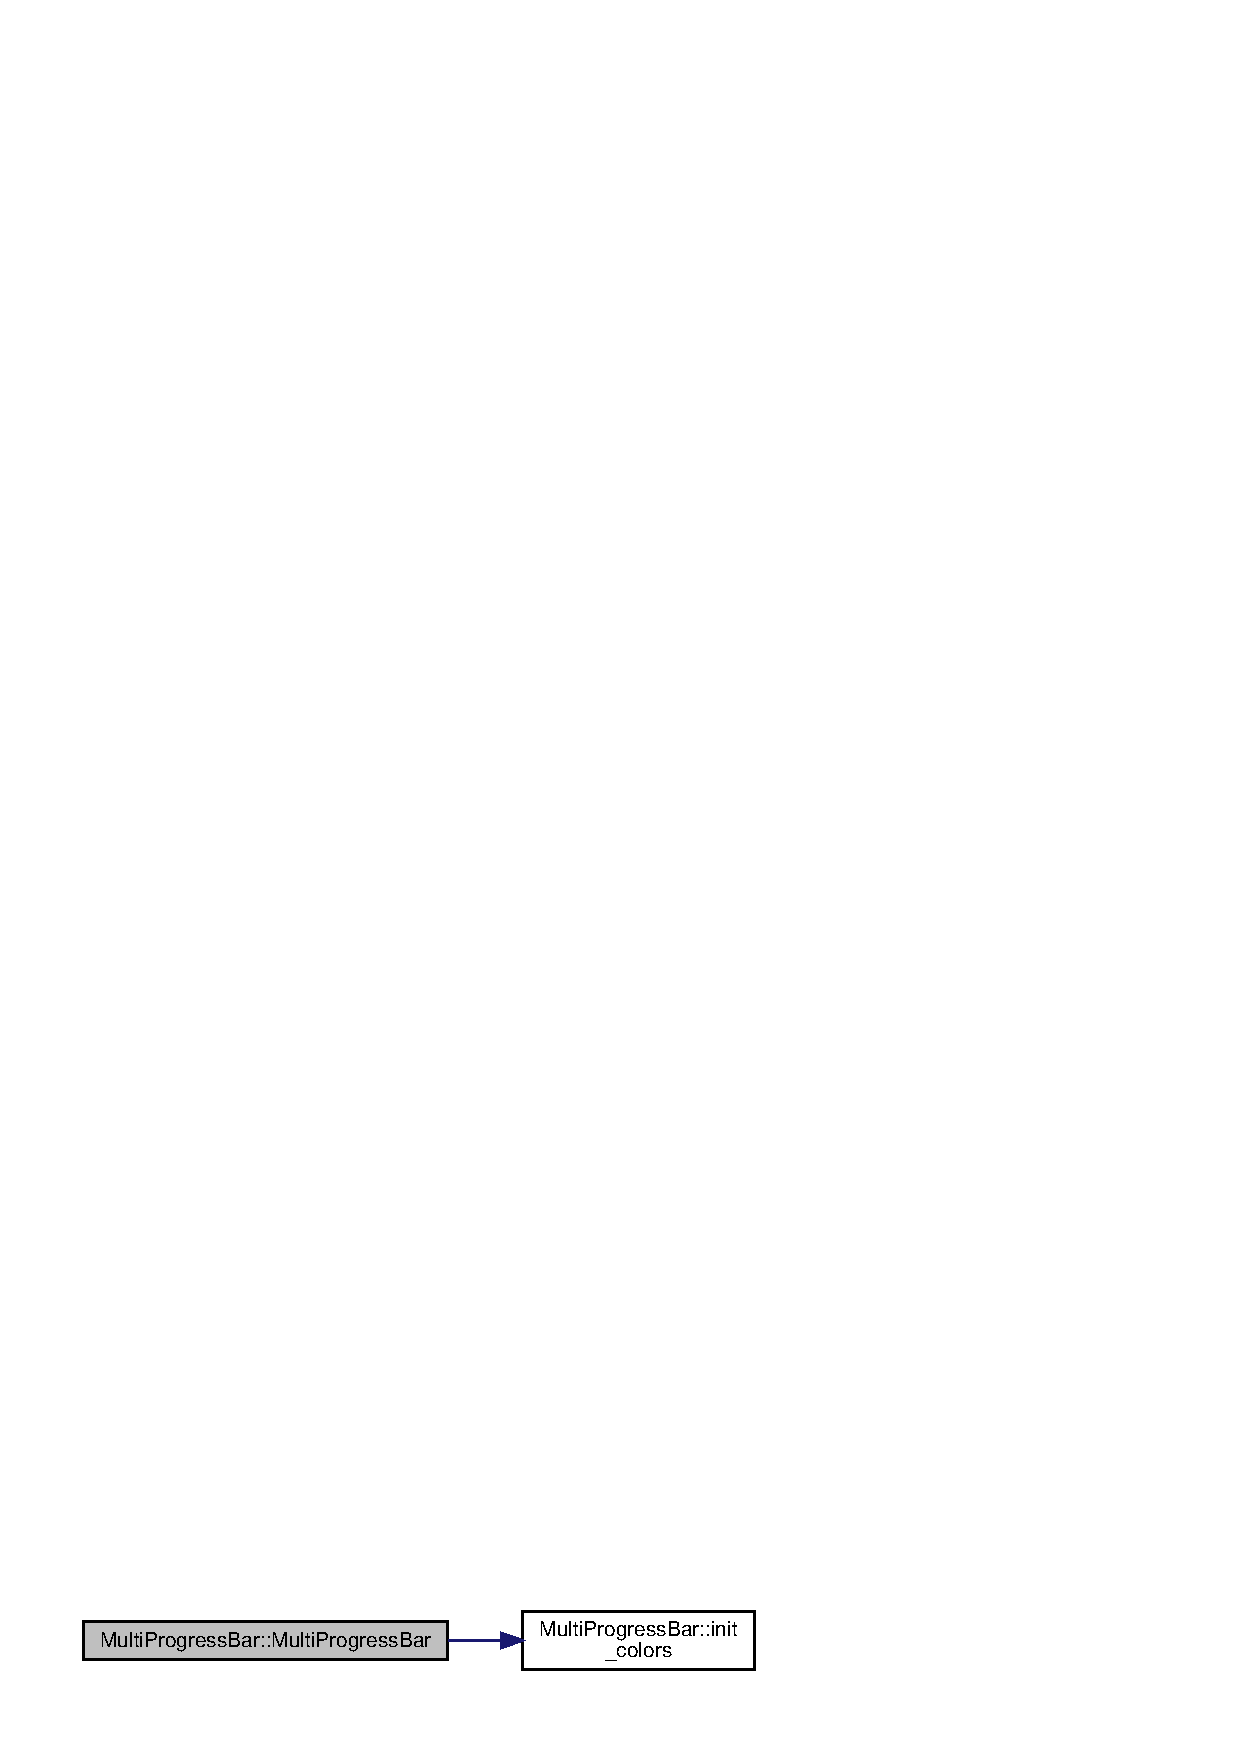
\includegraphics[width=350pt]{classMultiProgressBar_aaab5d64069e511a0c5c5f029936506d7_aaab5d64069e511a0c5c5f029936506d7_cgraph}
\end{center}
\end{figure}
\mbox{\label{classMultiProgressBar_a192362044eb0b1f9955a6bd824300a7c_a192362044eb0b1f9955a6bd824300a7c}} 
\index{Multi\+Progress\+Bar@{Multi\+Progress\+Bar}!Multi\+Progress\+Bar@{Multi\+Progress\+Bar}}
\index{Multi\+Progress\+Bar@{Multi\+Progress\+Bar}!Multi\+Progress\+Bar@{Multi\+Progress\+Bar}}
\subsubsection{Multi\+Progress\+Bar()\hspace{0.1cm}{\footnotesize\ttfamily [2/2]}}
{\footnotesize\ttfamily Multi\+Progress\+Bar\+::\+Multi\+Progress\+Bar (\begin{DoxyParamCaption}\item[{double}]{total,  }\item[{int}]{color = {\ttfamily 0} }\end{DoxyParamCaption})}



Definition at line 16 of file Multi\+Progress\+Bar.\+cpp.



References init\+\_\+colors(), m\+\_\+bar\+\_\+char\+\_\+right, m\+\_\+bar\+\_\+str, m\+\_\+current\+\_\+index, m\+\_\+factor, m\+\_\+left, m\+\_\+length\+\_\+bar, m\+\_\+percent, m\+\_\+right, m\+\_\+title, and m\+\_\+total.

Here is the call graph for this function\+:\nopagebreak
\begin{figure}[H]
\begin{center}
\leavevmode
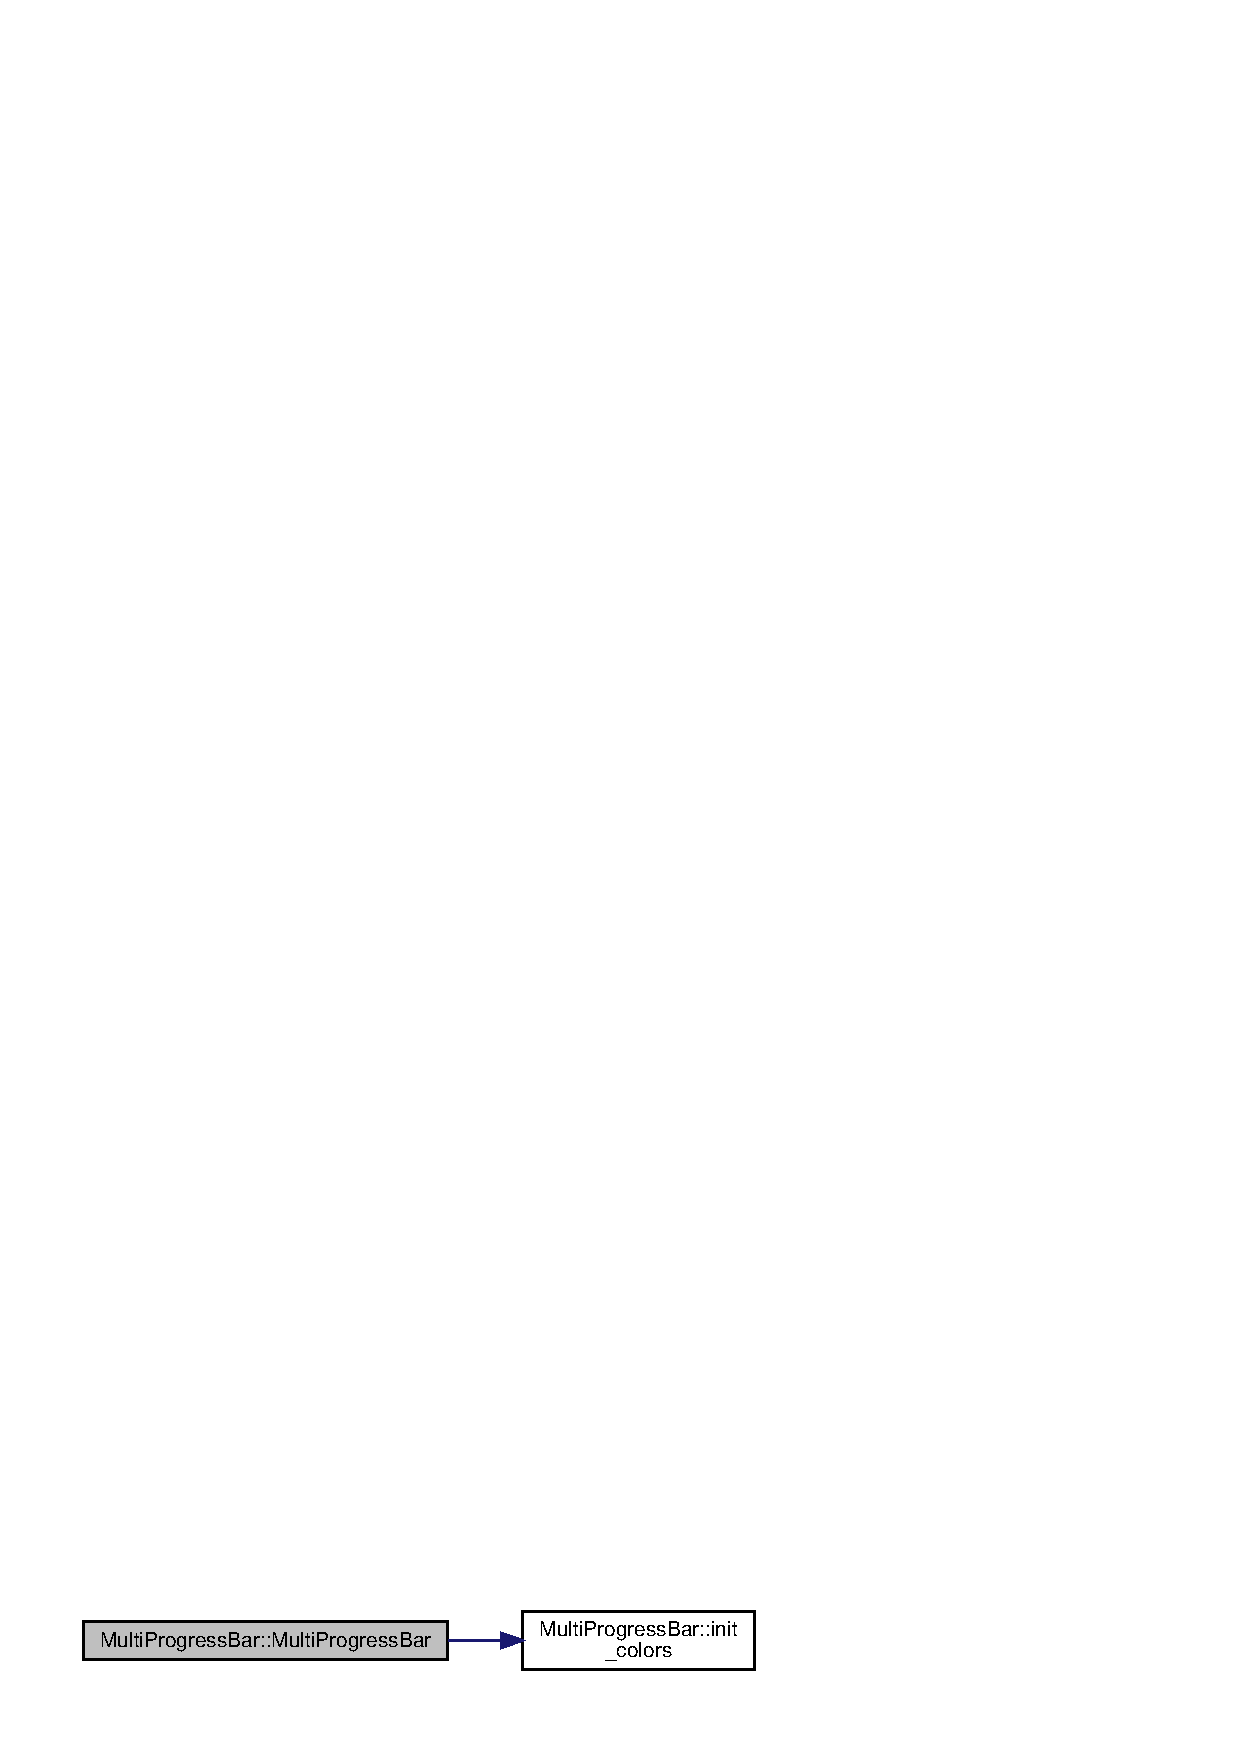
\includegraphics[width=350pt]{classMultiProgressBar_a192362044eb0b1f9955a6bd824300a7c_a192362044eb0b1f9955a6bd824300a7c_cgraph}
\end{center}
\end{figure}
\mbox{\label{classMultiProgressBar_aa6447c0d66c0f765f11c920863fa71ad_aa6447c0d66c0f765f11c920863fa71ad}} 
\index{Multi\+Progress\+Bar@{Multi\+Progress\+Bar}!````~Multi\+Progress\+Bar@{$\sim$\+Multi\+Progress\+Bar}}
\index{````~Multi\+Progress\+Bar@{$\sim$\+Multi\+Progress\+Bar}!Multi\+Progress\+Bar@{Multi\+Progress\+Bar}}
\subsubsection{$\sim$\+Multi\+Progress\+Bar()}
{\footnotesize\ttfamily Multi\+Progress\+Bar\+::$\sim$\+Multi\+Progress\+Bar (\begin{DoxyParamCaption}{ }\end{DoxyParamCaption})}



Definition at line 13 of file Multi\+Progress\+Bar.\+cpp.



\subsection{Member Function Documentation}
\mbox{\label{classMultiProgressBar_ab6dc669eb38eecf874db34f4237418fb_ab6dc669eb38eecf874db34f4237418fb}} 
\index{Multi\+Progress\+Bar@{Multi\+Progress\+Bar}!init\+\_\+colors@{init\+\_\+colors}}
\index{init\+\_\+colors@{init\+\_\+colors}!Multi\+Progress\+Bar@{Multi\+Progress\+Bar}}
\subsubsection{init\+\_\+colors()}
{\footnotesize\ttfamily void Multi\+Progress\+Bar\+::init\+\_\+colors (\begin{DoxyParamCaption}{ }\end{DoxyParamCaption})\hspace{0.3cm}{\ttfamily [private]}}



Definition at line 5 of file Multi\+Progress\+Bar.\+cpp.



References m\+\_\+colors.



Referenced by Multi\+Progress\+Bar().

Here is the caller graph for this function\+:\nopagebreak
\begin{figure}[H]
\begin{center}
\leavevmode
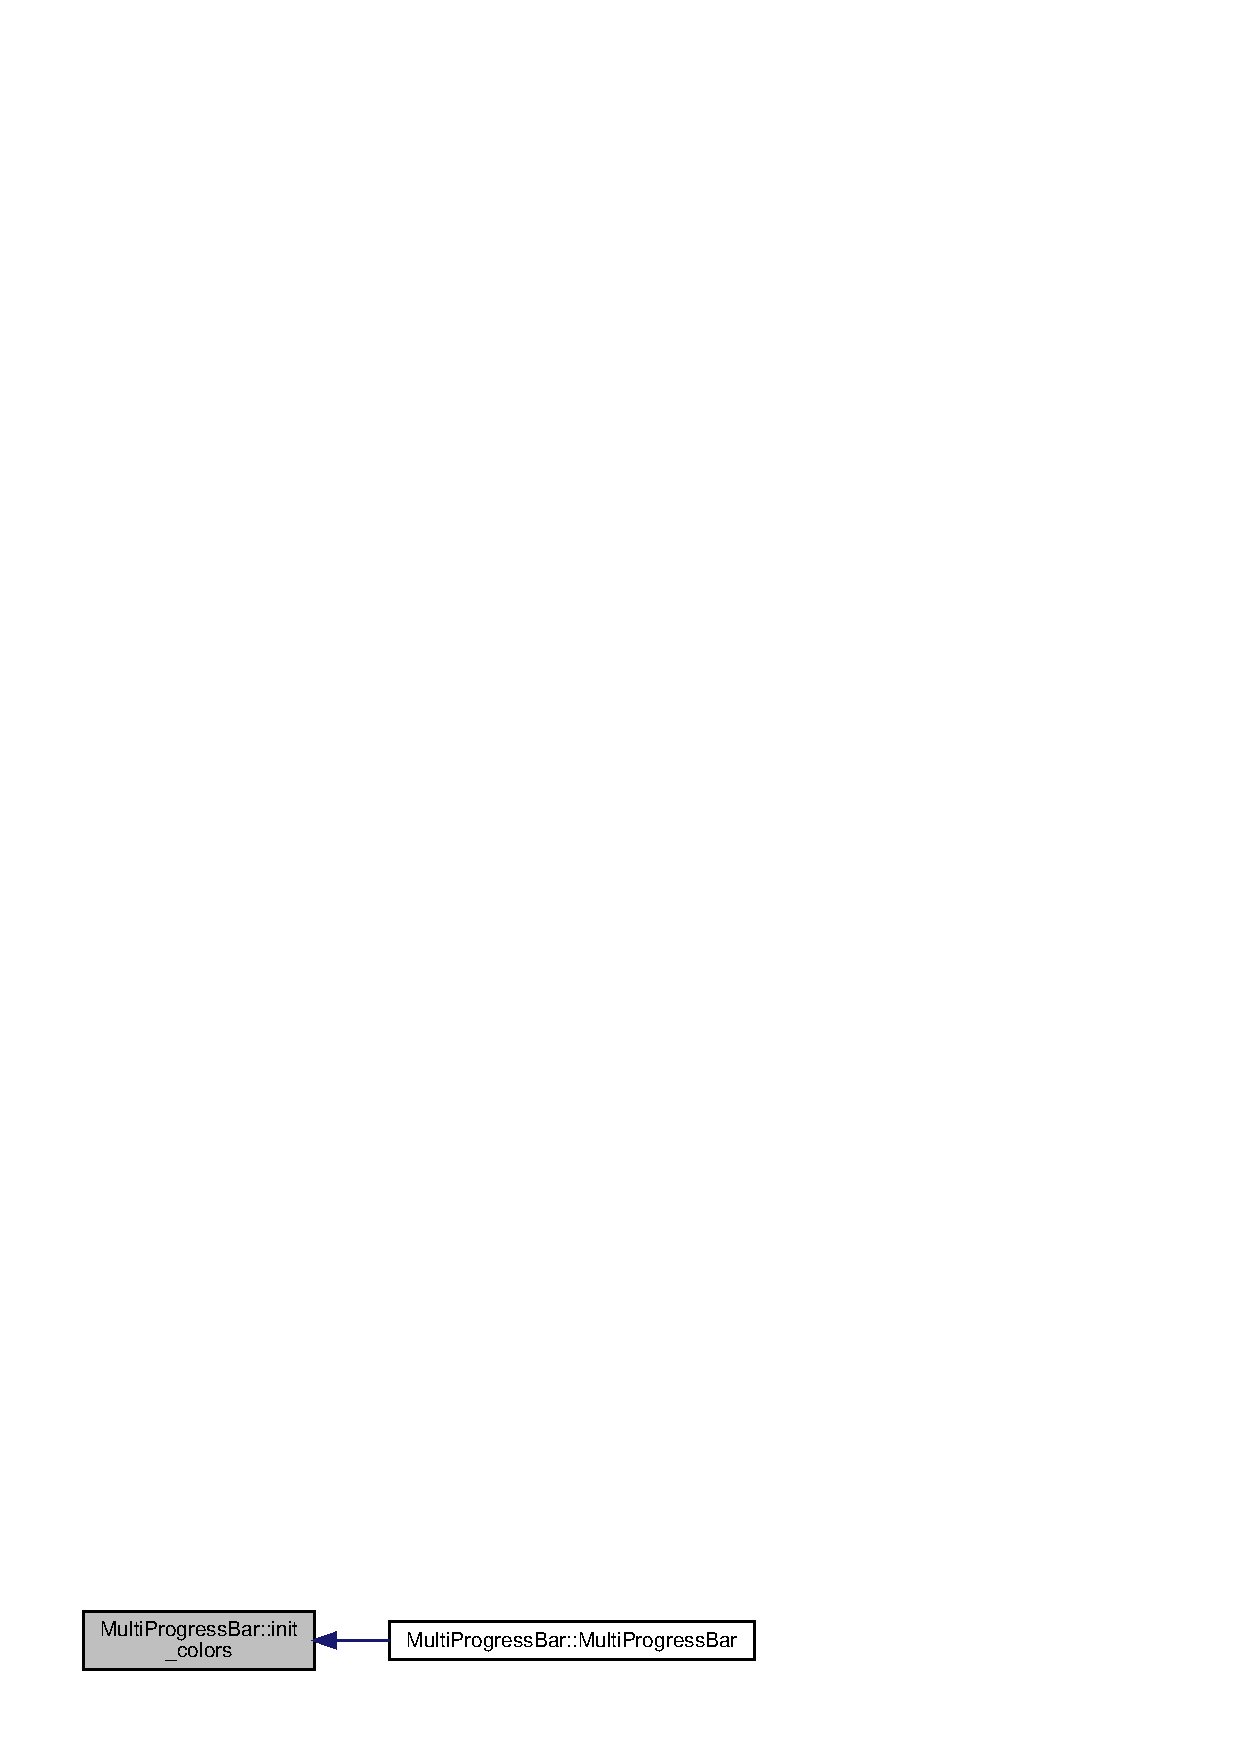
\includegraphics[width=350pt]{classMultiProgressBar_ab6dc669eb38eecf874db34f4237418fb_ab6dc669eb38eecf874db34f4237418fb_icgraph}
\end{center}
\end{figure}
\mbox{\label{classMultiProgressBar_a58eef55ad6d5c7d769b3a402a2ef7b85_a58eef55ad6d5c7d769b3a402a2ef7b85}} 
\index{Multi\+Progress\+Bar@{Multi\+Progress\+Bar}!Update@{Update}}
\index{Update@{Update}!Multi\+Progress\+Bar@{Multi\+Progress\+Bar}}
\subsubsection{Update()\hspace{0.1cm}{\footnotesize\ttfamily [1/2]}}
{\footnotesize\ttfamily void Multi\+Progress\+Bar\+::\+Update (\begin{DoxyParamCaption}\item[{double}]{current\+\_\+pos = {\ttfamily -\/1} }\end{DoxyParamCaption})}



Definition at line 76 of file Multi\+Progress\+Bar.\+cpp.



References m\+\_\+current\+\_\+index, and m\+\_\+total.



Referenced by D\+W\+C\+\_\+p2p\+\_\+\+C\+G\+L\+S(), D\+W\+C\+\_\+p2p\+\_\+\+Itegration\+Iter(), D\+W\+C\+\_\+p2p\+\_\+\+Landweber\+Iter(), D\+W\+C\+\_\+s2p\+\_\+\+C\+G\+L\+S(), D\+W\+C\+\_\+s2p\+\_\+\+Itegration\+Iter(), D\+W\+C\+\_\+s2p\+\_\+\+Landweber\+Iter(), D\+W\+C\+\_\+s2p\+\_\+\+Tikhonov(), Getkernel\+\_\+p2p(), Getkernel\+\_\+p2p\+\_\+new(), and Getkernel\+\_\+p2s\+\_\+new().

Here is the caller graph for this function\+:
\nopagebreak
\begin{figure}[H]
\begin{center}
\leavevmode
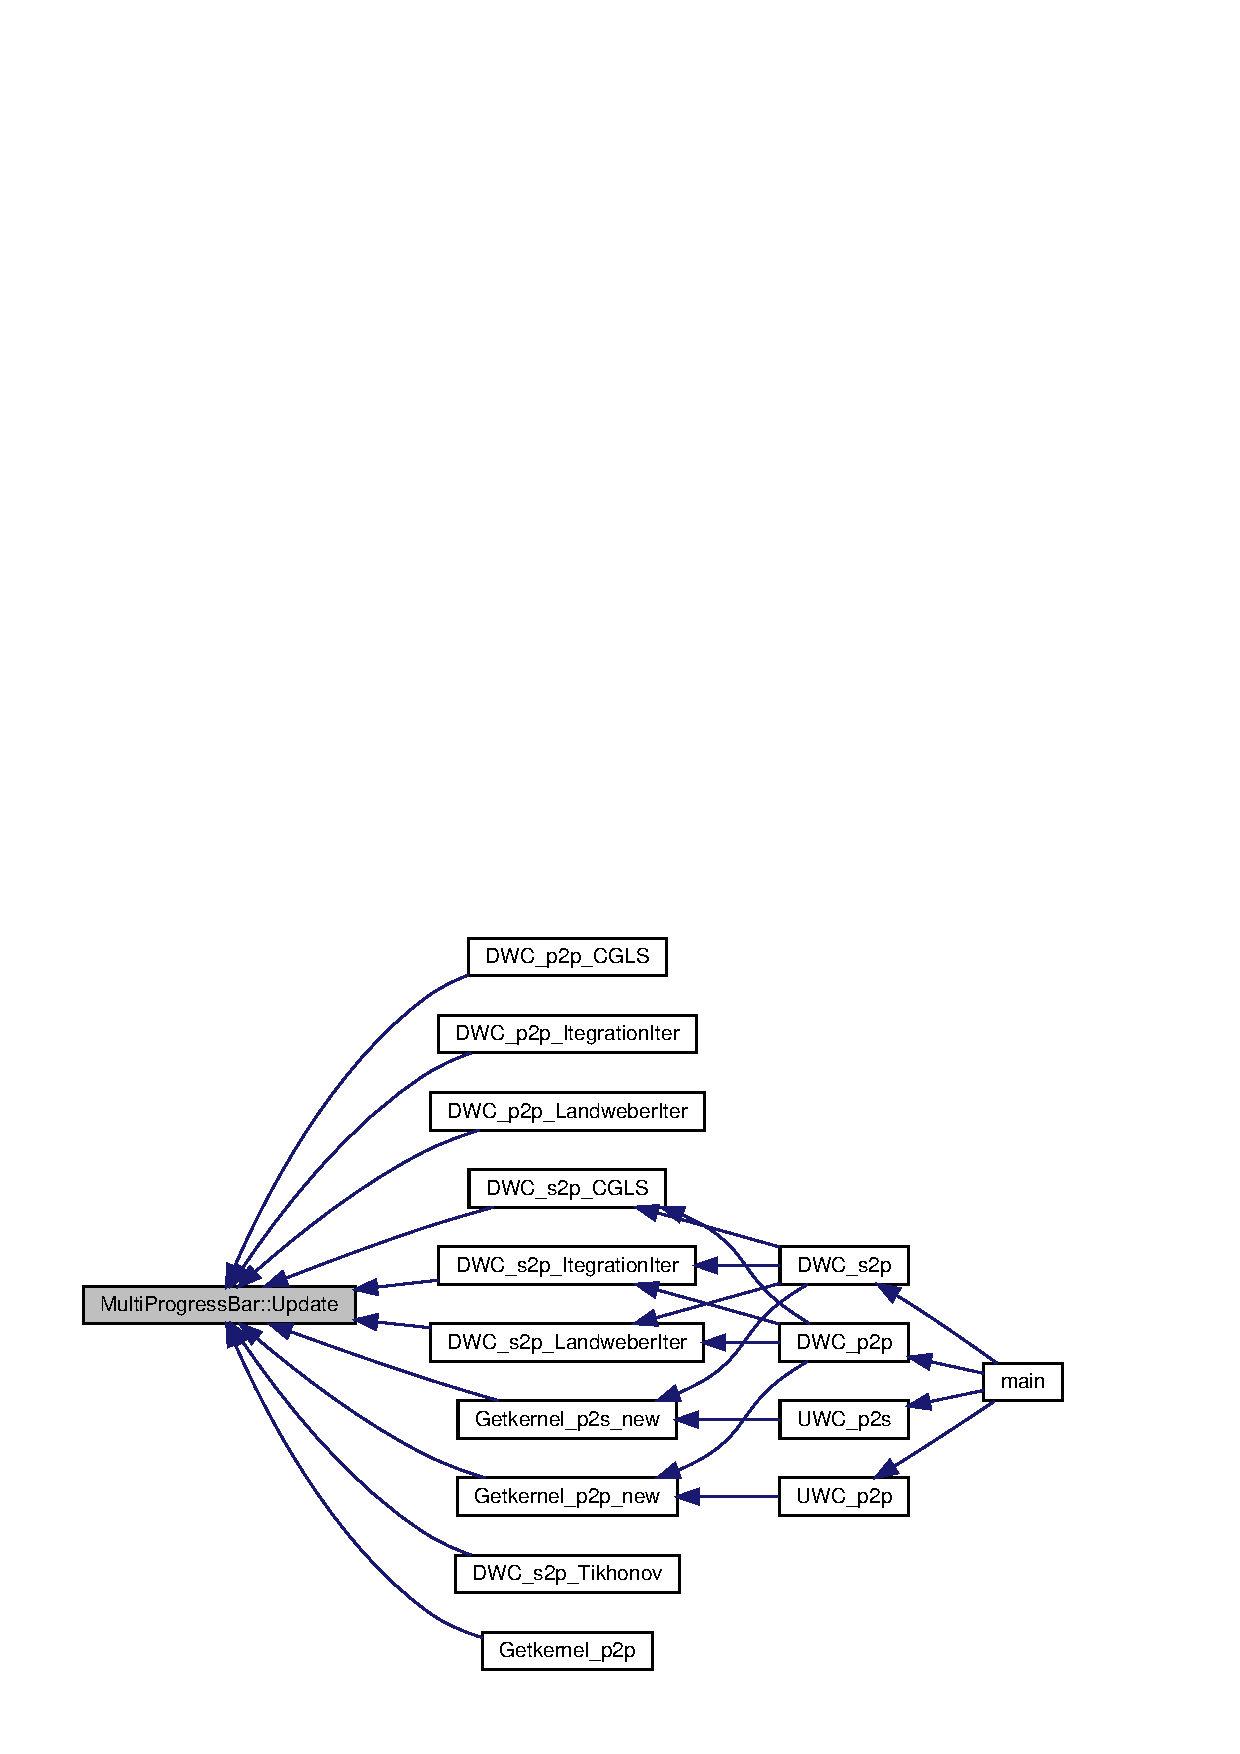
\includegraphics[width=350pt]{classMultiProgressBar_a58eef55ad6d5c7d769b3a402a2ef7b85_a58eef55ad6d5c7d769b3a402a2ef7b85_icgraph}
\end{center}
\end{figure}
\mbox{\label{classMultiProgressBar_abf5be627ae86f33f482125ce2e4370c7_abf5be627ae86f33f482125ce2e4370c7}} 
\index{Multi\+Progress\+Bar@{Multi\+Progress\+Bar}!Update@{Update}}
\index{Update@{Update}!Multi\+Progress\+Bar@{Multi\+Progress\+Bar}}
\subsubsection{Update()\hspace{0.1cm}{\footnotesize\ttfamily [2/2]}}
{\footnotesize\ttfamily void Multi\+Progress\+Bar\+::\+Update (\begin{DoxyParamCaption}\item[{vector$<$ double $>$}]{current\+\_\+pos }\end{DoxyParamCaption})}



Definition at line 84 of file Multi\+Progress\+Bar.\+cpp.



References C\+O\+L\+O\+R\+\_\+\+D\+E\+F\+A\+L\+UT, m\+\_\+bar\+\_\+char\+\_\+left, m\+\_\+bar\+\_\+char\+\_\+right, m\+\_\+bar\+\_\+str, m\+\_\+colors, m\+\_\+defaultcolor, m\+\_\+factor, m\+\_\+left, m\+\_\+length\+\_\+bar, m\+\_\+max\+Length\+\_\+title, m\+\_\+percent, m\+\_\+title, m\+\_\+total, and M\+O\+V\+E\+UP.



\subsection{Member Data Documentation}
\mbox{\label{classMultiProgressBar_a0988d7a44c4eb92aa791b73ed0a5c040_a0988d7a44c4eb92aa791b73ed0a5c040}} 
\index{Multi\+Progress\+Bar@{Multi\+Progress\+Bar}!m\+\_\+bar\+\_\+char\+\_\+left@{m\+\_\+bar\+\_\+char\+\_\+left}}
\index{m\+\_\+bar\+\_\+char\+\_\+left@{m\+\_\+bar\+\_\+char\+\_\+left}!Multi\+Progress\+Bar@{Multi\+Progress\+Bar}}
\subsubsection{m\+\_\+bar\+\_\+char\+\_\+left}
{\footnotesize\ttfamily char Multi\+Progress\+Bar\+::m\+\_\+bar\+\_\+char\+\_\+left\hspace{0.3cm}{\ttfamily [protected]}}



Definition at line 25 of file Multi\+Progress\+Bar.\+h.



Referenced by Update().

\mbox{\label{classMultiProgressBar_afaae2b720a00fd64a4a8298dba36268c_afaae2b720a00fd64a4a8298dba36268c}} 
\index{Multi\+Progress\+Bar@{Multi\+Progress\+Bar}!m\+\_\+bar\+\_\+char\+\_\+right@{m\+\_\+bar\+\_\+char\+\_\+right}}
\index{m\+\_\+bar\+\_\+char\+\_\+right@{m\+\_\+bar\+\_\+char\+\_\+right}!Multi\+Progress\+Bar@{Multi\+Progress\+Bar}}
\subsubsection{m\+\_\+bar\+\_\+char\+\_\+right}
{\footnotesize\ttfamily char Multi\+Progress\+Bar\+::m\+\_\+bar\+\_\+char\+\_\+right\hspace{0.3cm}{\ttfamily [protected]}}



Definition at line 26 of file Multi\+Progress\+Bar.\+h.



Referenced by Multi\+Progress\+Bar(), and Update().

\mbox{\label{classMultiProgressBar_a1a3803e31fc7bc086854ab6f1c6e7667_a1a3803e31fc7bc086854ab6f1c6e7667}} 
\index{Multi\+Progress\+Bar@{Multi\+Progress\+Bar}!m\+\_\+bar\+\_\+number@{m\+\_\+bar\+\_\+number}}
\index{m\+\_\+bar\+\_\+number@{m\+\_\+bar\+\_\+number}!Multi\+Progress\+Bar@{Multi\+Progress\+Bar}}
\subsubsection{m\+\_\+bar\+\_\+number}
{\footnotesize\ttfamily int Multi\+Progress\+Bar\+::m\+\_\+bar\+\_\+number\hspace{0.3cm}{\ttfamily [protected]}}



Definition at line 31 of file Multi\+Progress\+Bar.\+h.

\mbox{\label{classMultiProgressBar_af35a7ef9e9f8f6078cd053d4c1c57c13_af35a7ef9e9f8f6078cd053d4c1c57c13}} 
\index{Multi\+Progress\+Bar@{Multi\+Progress\+Bar}!m\+\_\+bar\+\_\+str@{m\+\_\+bar\+\_\+str}}
\index{m\+\_\+bar\+\_\+str@{m\+\_\+bar\+\_\+str}!Multi\+Progress\+Bar@{Multi\+Progress\+Bar}}
\subsubsection{m\+\_\+bar\+\_\+str}
{\footnotesize\ttfamily vector$<$string$>$ Multi\+Progress\+Bar\+::m\+\_\+bar\+\_\+str\hspace{0.3cm}{\ttfamily [protected]}}



Definition at line 23 of file Multi\+Progress\+Bar.\+h.



Referenced by Multi\+Progress\+Bar(), and Update().

\mbox{\label{classMultiProgressBar_a4a81485c32d529951d4f7ad2962fe990_a4a81485c32d529951d4f7ad2962fe990}} 
\index{Multi\+Progress\+Bar@{Multi\+Progress\+Bar}!m\+\_\+colors@{m\+\_\+colors}}
\index{m\+\_\+colors@{m\+\_\+colors}!Multi\+Progress\+Bar@{Multi\+Progress\+Bar}}
\subsubsection{m\+\_\+colors}
{\footnotesize\ttfamily vector$<$string$>$ Multi\+Progress\+Bar\+::m\+\_\+colors\hspace{0.3cm}{\ttfamily [private]}}



Definition at line 36 of file Multi\+Progress\+Bar.\+h.



Referenced by init\+\_\+colors(), and Update().

\mbox{\label{classMultiProgressBar_a3810b1b4f80f6430a19fd3f699072f66_a3810b1b4f80f6430a19fd3f699072f66}} 
\index{Multi\+Progress\+Bar@{Multi\+Progress\+Bar}!m\+\_\+current\+\_\+index@{m\+\_\+current\+\_\+index}}
\index{m\+\_\+current\+\_\+index@{m\+\_\+current\+\_\+index}!Multi\+Progress\+Bar@{Multi\+Progress\+Bar}}
\subsubsection{m\+\_\+current\+\_\+index}
{\footnotesize\ttfamily vector$<$double$>$ Multi\+Progress\+Bar\+::m\+\_\+current\+\_\+index\hspace{0.3cm}{\ttfamily [protected]}}



Definition at line 30 of file Multi\+Progress\+Bar.\+h.



Referenced by Multi\+Progress\+Bar(), and Update().

\mbox{\label{classMultiProgressBar_a0feeb1e41adf9e50b2b25e70a39fddb5_a0feeb1e41adf9e50b2b25e70a39fddb5}} 
\index{Multi\+Progress\+Bar@{Multi\+Progress\+Bar}!m\+\_\+defaultcolor@{m\+\_\+defaultcolor}}
\index{m\+\_\+defaultcolor@{m\+\_\+defaultcolor}!Multi\+Progress\+Bar@{Multi\+Progress\+Bar}}
\subsubsection{m\+\_\+defaultcolor}
{\footnotesize\ttfamily int Multi\+Progress\+Bar\+::m\+\_\+defaultcolor\hspace{0.3cm}{\ttfamily [private]}}



Definition at line 38 of file Multi\+Progress\+Bar.\+h.



Referenced by Update().

\mbox{\label{classMultiProgressBar_a3befa397116ae560dd86250d5caada4d_a3befa397116ae560dd86250d5caada4d}} 
\index{Multi\+Progress\+Bar@{Multi\+Progress\+Bar}!m\+\_\+factor@{m\+\_\+factor}}
\index{m\+\_\+factor@{m\+\_\+factor}!Multi\+Progress\+Bar@{Multi\+Progress\+Bar}}
\subsubsection{m\+\_\+factor}
{\footnotesize\ttfamily double Multi\+Progress\+Bar\+::m\+\_\+factor\hspace{0.3cm}{\ttfamily [private]}}



Definition at line 35 of file Multi\+Progress\+Bar.\+h.



Referenced by Multi\+Progress\+Bar(), and Update().

\mbox{\label{classMultiProgressBar_af1ad5d5306597de5925d69ceda22d3a5_af1ad5d5306597de5925d69ceda22d3a5}} 
\index{Multi\+Progress\+Bar@{Multi\+Progress\+Bar}!m\+\_\+left@{m\+\_\+left}}
\index{m\+\_\+left@{m\+\_\+left}!Multi\+Progress\+Bar@{Multi\+Progress\+Bar}}
\subsubsection{m\+\_\+left}
{\footnotesize\ttfamily vector$<$double$>$ Multi\+Progress\+Bar\+::m\+\_\+left\hspace{0.3cm}{\ttfamily [protected]}}



Definition at line 32 of file Multi\+Progress\+Bar.\+h.



Referenced by Multi\+Progress\+Bar(), and Update().

\mbox{\label{classMultiProgressBar_a0319176f9fc1a3443c2e7d76163d6401_a0319176f9fc1a3443c2e7d76163d6401}} 
\index{Multi\+Progress\+Bar@{Multi\+Progress\+Bar}!m\+\_\+length\+\_\+bar@{m\+\_\+length\+\_\+bar}}
\index{m\+\_\+length\+\_\+bar@{m\+\_\+length\+\_\+bar}!Multi\+Progress\+Bar@{Multi\+Progress\+Bar}}
\subsubsection{m\+\_\+length\+\_\+bar}
{\footnotesize\ttfamily int Multi\+Progress\+Bar\+::m\+\_\+length\+\_\+bar\hspace{0.3cm}{\ttfamily [protected]}}



Definition at line 24 of file Multi\+Progress\+Bar.\+h.



Referenced by Multi\+Progress\+Bar(), and Update().

\mbox{\label{classMultiProgressBar_a12795fa634323457d1cacfc8a2beec12_a12795fa634323457d1cacfc8a2beec12}} 
\index{Multi\+Progress\+Bar@{Multi\+Progress\+Bar}!m\+\_\+max\+Length\+\_\+title@{m\+\_\+max\+Length\+\_\+title}}
\index{m\+\_\+max\+Length\+\_\+title@{m\+\_\+max\+Length\+\_\+title}!Multi\+Progress\+Bar@{Multi\+Progress\+Bar}}
\subsubsection{m\+\_\+max\+Length\+\_\+title}
{\footnotesize\ttfamily int Multi\+Progress\+Bar\+::m\+\_\+max\+Length\+\_\+title\hspace{0.3cm}{\ttfamily [protected]}}



Definition at line 33 of file Multi\+Progress\+Bar.\+h.



Referenced by Multi\+Progress\+Bar(), and Update().

\mbox{\label{classMultiProgressBar_a4776b46fbbea37fb83caedbe8e45a5e1_a4776b46fbbea37fb83caedbe8e45a5e1}} 
\index{Multi\+Progress\+Bar@{Multi\+Progress\+Bar}!m\+\_\+percent@{m\+\_\+percent}}
\index{m\+\_\+percent@{m\+\_\+percent}!Multi\+Progress\+Bar@{Multi\+Progress\+Bar}}
\subsubsection{m\+\_\+percent}
{\footnotesize\ttfamily vector$<$double$>$ Multi\+Progress\+Bar\+::m\+\_\+percent\hspace{0.3cm}{\ttfamily [protected]}}



Definition at line 27 of file Multi\+Progress\+Bar.\+h.



Referenced by Multi\+Progress\+Bar(), and Update().

\mbox{\label{classMultiProgressBar_a5cf91e4bca7a5959e9abd67a398389dc_a5cf91e4bca7a5959e9abd67a398389dc}} 
\index{Multi\+Progress\+Bar@{Multi\+Progress\+Bar}!m\+\_\+right@{m\+\_\+right}}
\index{m\+\_\+right@{m\+\_\+right}!Multi\+Progress\+Bar@{Multi\+Progress\+Bar}}
\subsubsection{m\+\_\+right}
{\footnotesize\ttfamily vector$<$double$>$ Multi\+Progress\+Bar\+::m\+\_\+right\hspace{0.3cm}{\ttfamily [protected]}}



Definition at line 32 of file Multi\+Progress\+Bar.\+h.



Referenced by Multi\+Progress\+Bar().

\mbox{\label{classMultiProgressBar_a1e81427871e1604a72672eed3cc1a476_a1e81427871e1604a72672eed3cc1a476}} 
\index{Multi\+Progress\+Bar@{Multi\+Progress\+Bar}!m\+\_\+title@{m\+\_\+title}}
\index{m\+\_\+title@{m\+\_\+title}!Multi\+Progress\+Bar@{Multi\+Progress\+Bar}}
\subsubsection{m\+\_\+title}
{\footnotesize\ttfamily vector$<$string$>$ Multi\+Progress\+Bar\+::m\+\_\+title\hspace{0.3cm}{\ttfamily [protected]}}



Definition at line 28 of file Multi\+Progress\+Bar.\+h.



Referenced by Multi\+Progress\+Bar(), and Update().

\mbox{\label{classMultiProgressBar_a8abca9cff474835ccabbd7a93ddbfe99_a8abca9cff474835ccabbd7a93ddbfe99}} 
\index{Multi\+Progress\+Bar@{Multi\+Progress\+Bar}!m\+\_\+total@{m\+\_\+total}}
\index{m\+\_\+total@{m\+\_\+total}!Multi\+Progress\+Bar@{Multi\+Progress\+Bar}}
\subsubsection{m\+\_\+total}
{\footnotesize\ttfamily vector$<$double$>$ Multi\+Progress\+Bar\+::m\+\_\+total\hspace{0.3cm}{\ttfamily [protected]}}



Definition at line 29 of file Multi\+Progress\+Bar.\+h.



Referenced by Multi\+Progress\+Bar(), and Update().



The documentation for this class was generated from the following files\+:\begin{DoxyCompactItemize}
\item 
\textbf{ Multi\+Progress\+Bar.\+h}\item 
\textbf{ Multi\+Progress\+Bar.\+cpp}\end{DoxyCompactItemize}

\chapter{File Documentation}
\section{Conti2\+D.\+cpp File Reference}
\label{Conti2D_8cpp}\index{Conti2\+D.\+cpp@{Conti2\+D.\+cpp}}
{\ttfamily \#include \char`\"{}Conti2\+D.\+h\char`\"{}}\newline
Include dependency graph for Conti2\+D.\+cpp\+:\nopagebreak
\begin{figure}[H]
\begin{center}
\leavevmode
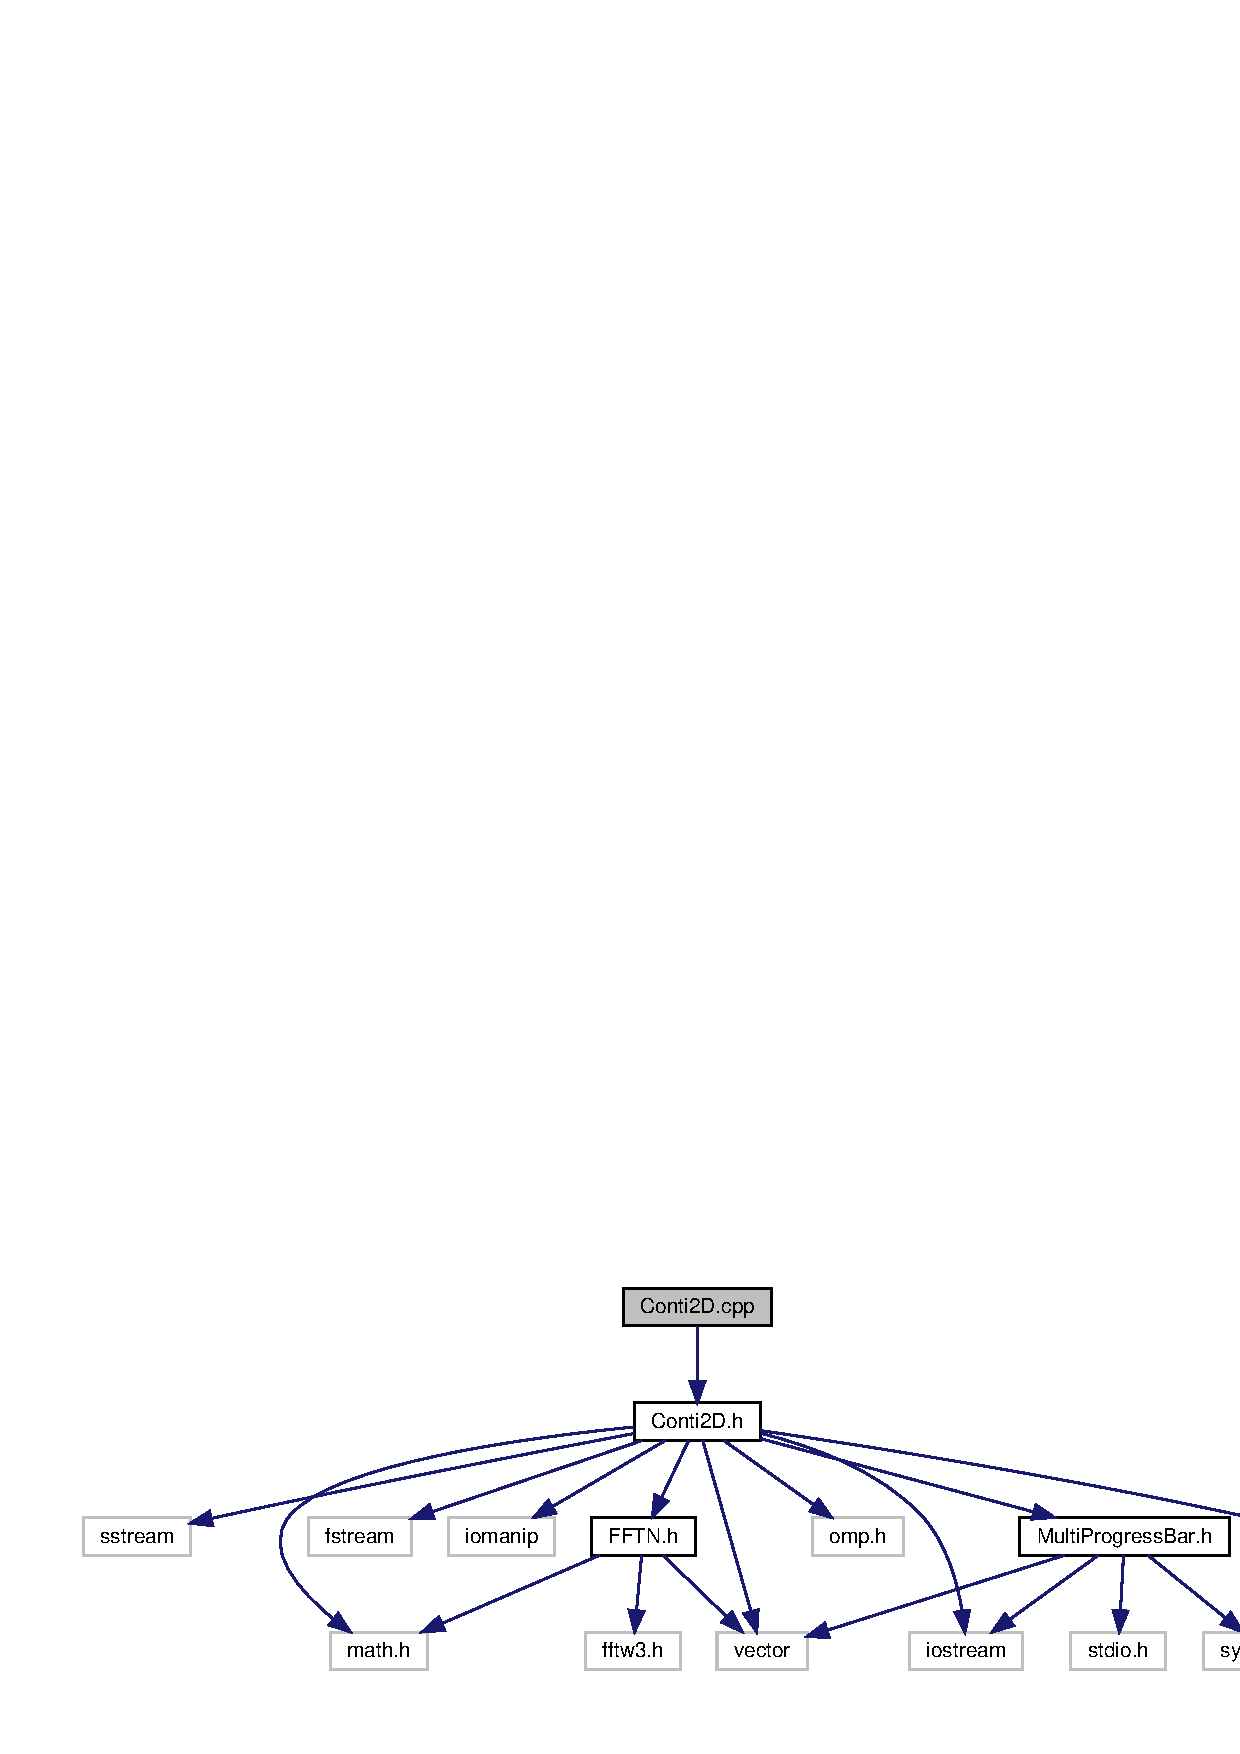
\includegraphics[width=350pt]{Conti2D_8cpp__incl}
\end{center}
\end{figure}
\subsection*{Functions}
\begin{DoxyCompactItemize}
\item 
string \textbf{ Path\+\_\+\+Get\+File\+Name} (string filepath)
\item 
string \textbf{ Path\+\_\+\+Get\+Path} (string filepath)
\item 
string \textbf{ Path\+\_\+\+Get\+Ext\+Name} (string filepath)
\item 
string \textbf{ Path\+\_\+\+Get\+Base\+Name} (string filepath)
\item 
void \textbf{ Get\+Kernal\+Matrix} (\textbf{ Grd\+Head} grdhead, double $\ast$G, const double rph, int num\+\_\+thread)
\begin{DoxyCompactList}\small\item\em Get the Kernal Matrix object. \end{DoxyCompactList}\item 
void \textbf{ Get\+Kernal\+Matrix\+\_\+new} (\textbf{ Grd\+Head} grdhead, double $\ast$G, const double rph, int num\+\_\+thread)
\begin{DoxyCompactList}\small\item\em Get the kernel matrix using the new developed formula. \end{DoxyCompactList}\item 
double \textbf{ Get\+Gij} (const int i, const int j, double $\ast$first\+Row, const \textbf{ Grd\+Head} grdhead)
\begin{DoxyCompactList}\small\item\em Get the value at i row and the j column of kernel matrix from the first row of the matrix only. \end{DoxyCompactList}\item 
void \textbf{ Get\+Pmnij} (double $\ast$Pmnij, int rows, int cols, double dx, double dy, double rph, double xm, double ym)
\item 
int \textbf{ Getkernel\+\_\+p2p} (\textbf{ Grd\+Head} grdhead, double rph, double $\ast$$\ast$kernel, int num\+\_\+thread)
\begin{DoxyCompactList}\small\item\em Upward continue from plane to plane. \end{DoxyCompactList}\item 
int \textbf{ Getkernel\+\_\+p2s\+\_\+new} (\textbf{ Grd\+Head} grdhead, double h1, double $\ast$topo2, double $\ast$$\ast$kernel, int num\+\_\+thread)
\item 
int \textbf{ Getkernel\+\_\+p2p\+\_\+new} (\textbf{ Grd\+Head} grdhead, double rph, double $\ast$$\ast$kernel, int num\+\_\+thread)
\item 
int \textbf{ Getkernel\+\_\+p2p\+\_\+new} (\textbf{ Grd\+Head} grdhead, double rph, double $\ast$kernel\+\_\+first\+Row, int num\+\_\+thread)
\item 
void \textbf{ U\+W\+C\+\_\+p2s} (string inputfilename, string outputfilename, double height1, string topo\+File, int ext\+Num, int num\+\_\+thread, bool is\+Progress, bool use\+Old\+Kernel, string filename\+\_\+exact)
\item 
void \textbf{ U\+W\+C\+\_\+p2p} (string inputfilename, string outputfilename, double height1, double height2, int ext\+Num, int num\+\_\+thread, bool is\+Progress, bool use\+Old\+Kernel, string filename\+\_\+exact)
\item 
void \textbf{ U\+W\+C\+\_\+p2p\+\_\+f} (string inputfilename, string outputfilename, double height1, double height2, int ext\+Num, string filename\+\_\+exact)
\item 
int \textbf{ U\+W\+C\+\_\+p2p\+\_\+f} (double $\ast$inputdata, double $\ast$result, \textbf{ Grd\+Head} grdhead, double rph)
\item 
int \textbf{ Getkernel\+\_\+u2p} (\textbf{ Grd\+Head} grdhead, double $\ast$terrain1, double height2, double $\ast$$\ast$kernel, int num\+\_\+thread)
\item 
int \textbf{ Getkernel\+\_\+u2p\+\_\+new} (\textbf{ Grd\+Head} grdhead, double $\ast$terrain1, double height2, double $\ast$nx, double $\ast$ny, double $\ast$nz, double $\ast$$\ast$kernel, int num\+\_\+thread)
\item 
double $\ast$ \textbf{ Read\+Grd} (string filename, \textbf{ Grd\+Head} \&grdhead, int ext\+Num)
\begin{DoxyCompactList}\small\item\em Read a Surfer Grid data from file. \end{DoxyCompactList}\item 
bool \textbf{ Save\+Grd} (string filename, \textbf{ Grd\+Head} grdhead, double $\ast$data, int ext\+Num, bool savexxyz, bool is\+Info)
\begin{DoxyCompactList}\small\item\em Save a Surfer Grid data to file. \end{DoxyCompactList}\item 
void \textbf{ U\+W\+C\+\_\+\+Gji} (double $\ast$b, double $\ast$$\ast$G, double $\ast$x, int modelnum, int num\+\_\+thread)
\item 
void \textbf{ U\+W\+C\+\_\+\+Gij} (double $\ast$b, double $\ast$$\ast$G, double $\ast$x, int modelnum, int num\+\_\+thread)
\item 
void \textbf{ U\+W\+C\+\_\+\+Gji} (double $\ast$b, double $\ast$G, double $\ast$x, \textbf{ Grd\+Head} grdhead, int num\+\_\+thread)
\item 
void \textbf{ U\+W\+C\+\_\+\+Gij} (double $\ast$b, double $\ast$G, double $\ast$x, \textbf{ Grd\+Head} grdhead, int num\+\_\+thread)
\item 
void \textbf{ U\+WC} (double $\ast$datain, double $\ast$dataout, \textbf{ Grd\+Head} grdhead, double $\ast$$\ast$G)
\item 
void \textbf{ D\+W\+C\+\_\+p2p\+\_\+f} (string inputfilename, string outputfilename, double height1, double height2, int ext\+Num, double T\+RP, int num\+\_\+thread, bool is\+Progress, bool use\+Old\+Kernel)
\item 
void \textbf{ D\+W\+C\+\_\+s2p} (string inputfilename, string outputfilename, string topo\+File, double height2, int ext\+Num, double D\+W\+C\+\_\+parameter, int D\+W\+C\+\_\+method, int num\+\_\+thread, bool is\+Progress, bool use\+Old\+Kernel, string filename\+\_\+exact)
\item 
void \textbf{ D\+W\+C\+\_\+s2p\+\_\+\+Itegration\+Iter} (double $\ast$$\ast$G, double $\ast$x, double $\ast$b, \textbf{ Grd\+Head} grdhead, int ext\+Num, int num\+\_\+thread, string outputfile, double iter\+\_\+number, double $\ast$Exact\+Solution)
\item 
void \textbf{ D\+W\+C\+\_\+p2p\+\_\+\+C\+G\+LS} (double $\ast$G\+\_\+first\+Row, double $\ast$x, double $\ast$b, \textbf{ Grd\+Head} grdhead, int ext\+Num, double delta, int num\+\_\+thread)
\item 
void \textbf{ D\+W\+C\+\_\+s2p\+\_\+\+C\+G\+LS} (double $\ast$$\ast$G, double $\ast$x, double $\ast$b, \textbf{ Grd\+Head} grdhead, int ext\+Num, double delta, int num\+\_\+thread)
\item 
void \textbf{ U\+W\+C\+\_\+\+G\+\_\+\+C\+G\+L\+S\+\_\+\+Tik} (double $\ast$b, double $\ast$$\ast$G, double $\ast$x, int modelnum, double lambda2, int num\+\_\+thread)
\item 
void \textbf{ D\+W\+C\+\_\+s2p\+\_\+\+Tikhonov} (double $\ast$$\ast$G, double $\ast$x, double $\ast$b0, \textbf{ Grd\+Head} grdhead, int ext\+Num, double lambda, int num\+\_\+thread)
\item 
void \textbf{ D\+W\+C\+\_\+p2p} (string inputfilename, string outputfilename, double height1, double height2, int ext\+Num, double D\+W\+C\+\_\+parameter, int D\+W\+C\+\_\+method, int num\+\_\+thread, bool is\+Progress, bool use\+Old\+Kernel, string filename\+\_\+exact)
\item 
void \textbf{ D\+W\+C\+\_\+p2p\+\_\+\+Itegration\+Iter} (double $\ast$G, double $\ast$x, double $\ast$b, \textbf{ Grd\+Head} grdhead, int ext\+Num, int num\+\_\+thread, string outputfile, double iter\+\_\+number, double $\ast$Exact\+Solution)
\item 
void \textbf{ D\+W\+C\+\_\+p2p\+\_\+\+Landweber\+Iter} (double $\ast$G, double $\ast$x, double $\ast$b, \textbf{ Grd\+Head} grdhead, int ext\+Num, int num\+\_\+thread, string outputfile, double iter\+\_\+number, double $\ast$Exact\+Solution)
\item 
void \textbf{ D\+W\+C\+\_\+s2p\+\_\+\+Landweber\+Iter} (double $\ast$$\ast$G, double $\ast$x, double $\ast$b, \textbf{ Grd\+Head} grdhead, int ext\+Num, int num\+\_\+thread, string outputfile, double iter\+\_\+number, double $\ast$Exact\+Solution)
\item 
void \textbf{ D\+W\+C\+\_\+\+Tikhonov\+\_\+old} (double $\ast$G\+\_\+first\+Row, double $\ast$dataout, double $\ast$indata, double T\+RP, int kmax, double daierta, \textbf{ Grd\+Head} grdhead, int num\+\_\+thread)
\item 
double \textbf{ Norm2} (double $\ast$x, const int num)
\item 
double \textbf{ Norm2\+\_\+\+Gradient} (double $\ast$result, \textbf{ Grd\+Head} grdhead)
\item 
int \textbf{ Save\+Grd2\+V\+TK} (string outputfile, \textbf{ Grd\+Head} grdhead, double $\ast$data)
\end{DoxyCompactItemize}


\subsection{Function Documentation}
\mbox{\label{Conti2D_8cpp_ab87ce573de93575b7ece2e4f772e03fd_ab87ce573de93575b7ece2e4f772e03fd}} 
\index{Conti2\+D.\+cpp@{Conti2\+D.\+cpp}!D\+W\+C\+\_\+p2p@{D\+W\+C\+\_\+p2p}}
\index{D\+W\+C\+\_\+p2p@{D\+W\+C\+\_\+p2p}!Conti2\+D.\+cpp@{Conti2\+D.\+cpp}}
\subsubsection{D\+W\+C\+\_\+p2p()}
{\footnotesize\ttfamily void D\+W\+C\+\_\+p2p (\begin{DoxyParamCaption}\item[{string}]{inputfilename,  }\item[{string}]{outputfilename,  }\item[{double}]{height1,  }\item[{double}]{height2,  }\item[{int}]{ext\+Num,  }\item[{double}]{D\+W\+C\+\_\+parameter,  }\item[{int}]{D\+W\+C\+\_\+method,  }\item[{int}]{num\+\_\+thread,  }\item[{bool}]{is\+Progress,  }\item[{bool}]{use\+Old\+Kernel,  }\item[{string}]{filename\+\_\+exact }\end{DoxyParamCaption})}



Definition at line 1669 of file Conti2\+D.\+cpp.



References Grd\+Head\+::bounds, C\+O\+L\+O\+R\+\_\+\+D\+E\+F\+A\+L\+UT, Grd\+Head\+::cols, D\+W\+C\+\_\+\+C\+G\+LS, D\+W\+C\+\_\+\+I\+N\+T\+E\+G\+R\+A\+L\+I\+T\+E\+R\+A\+T\+I\+ON, D\+W\+C\+\_\+\+L\+A\+N\+D\+W\+E\+B\+ER, D\+W\+C\+\_\+s2p\+\_\+\+C\+G\+L\+S(), D\+W\+C\+\_\+s2p\+\_\+\+Itegration\+Iter(), D\+W\+C\+\_\+s2p\+\_\+\+Landweber\+Iter(), D\+W\+C\+\_\+\+T\+I\+K\+H\+O\+N\+OV, Getkernel\+\_\+p2p\+\_\+new(), Read\+Grd(), R\+ED, Grd\+Head\+::rows, and Save\+Grd().



Referenced by main().

Here is the call graph for this function\+:
\nopagebreak
\begin{figure}[H]
\begin{center}
\leavevmode
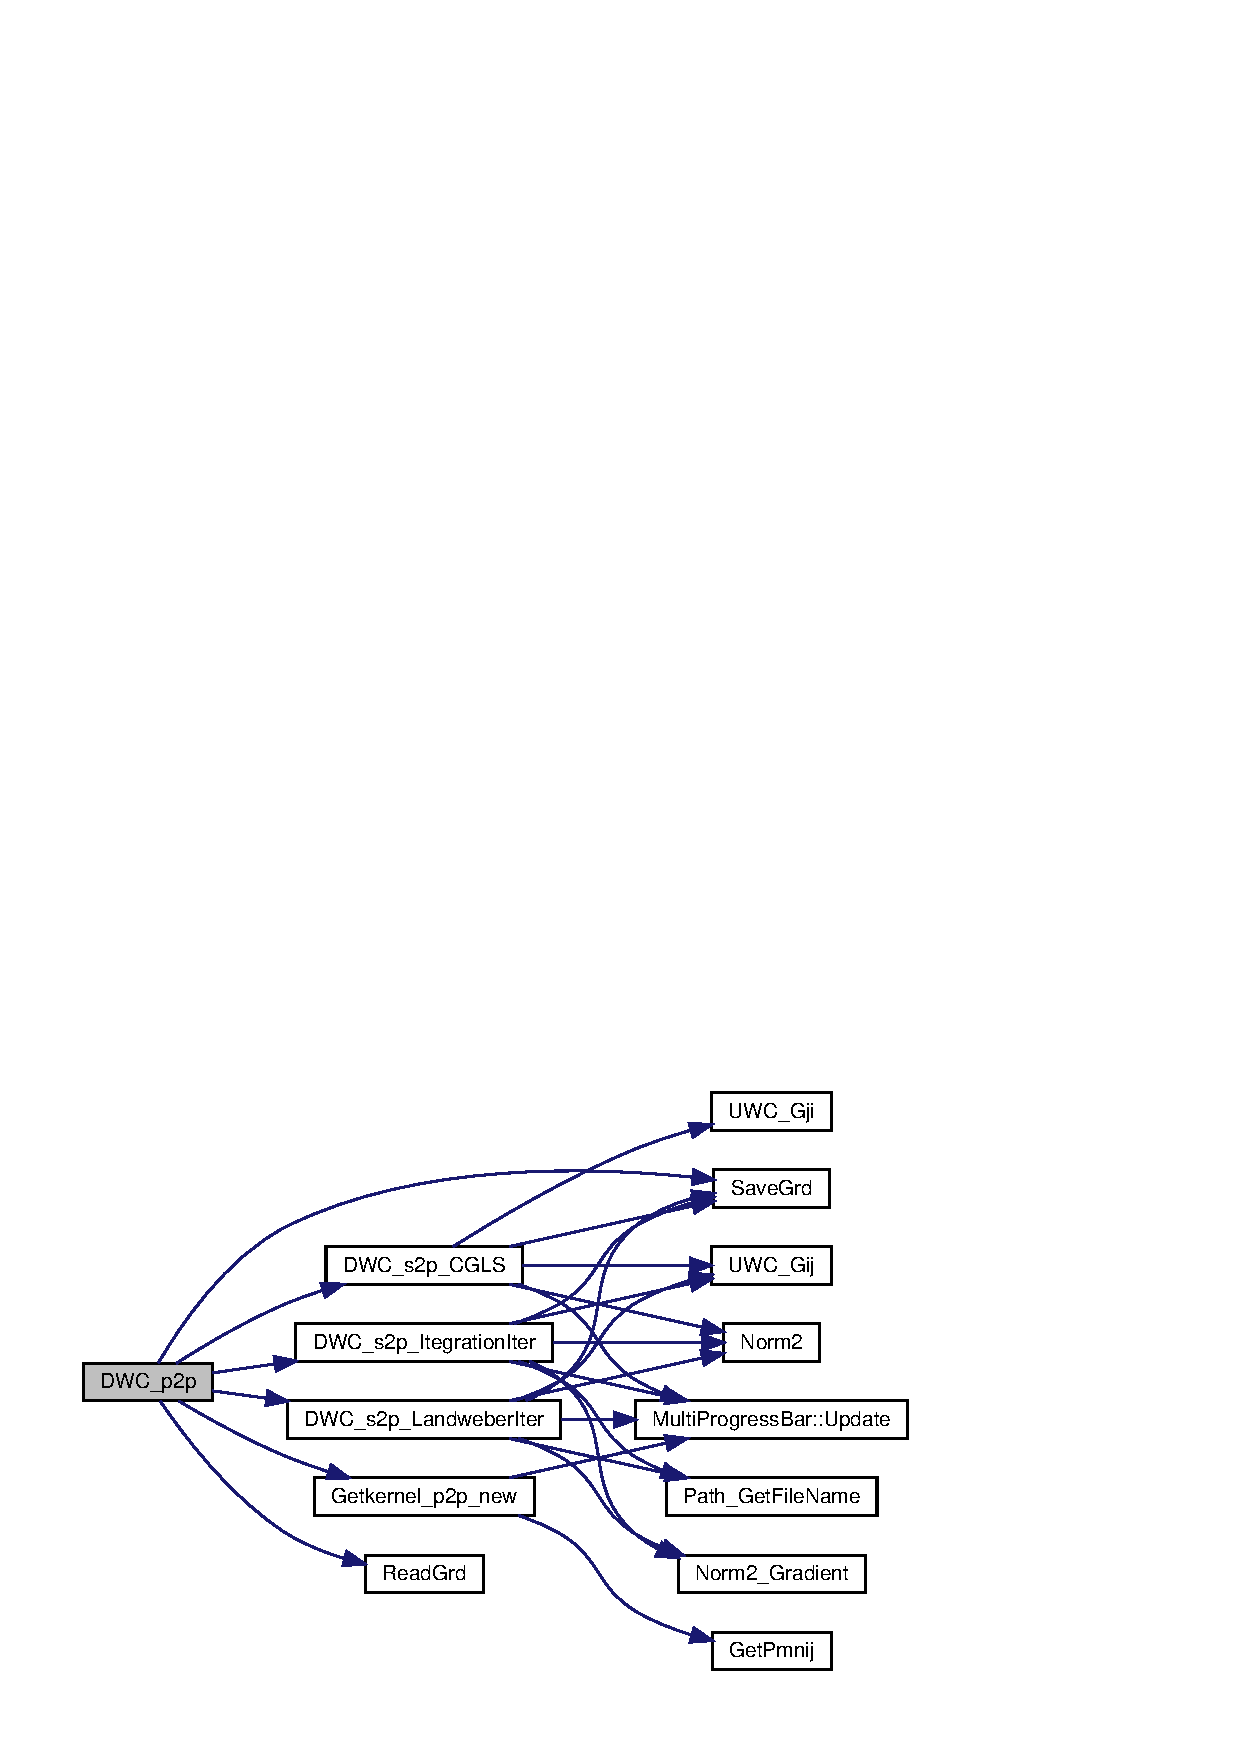
\includegraphics[width=350pt]{Conti2D_8cpp_ab87ce573de93575b7ece2e4f772e03fd_ab87ce573de93575b7ece2e4f772e03fd_cgraph}
\end{center}
\end{figure}
Here is the caller graph for this function\+:\nopagebreak
\begin{figure}[H]
\begin{center}
\leavevmode
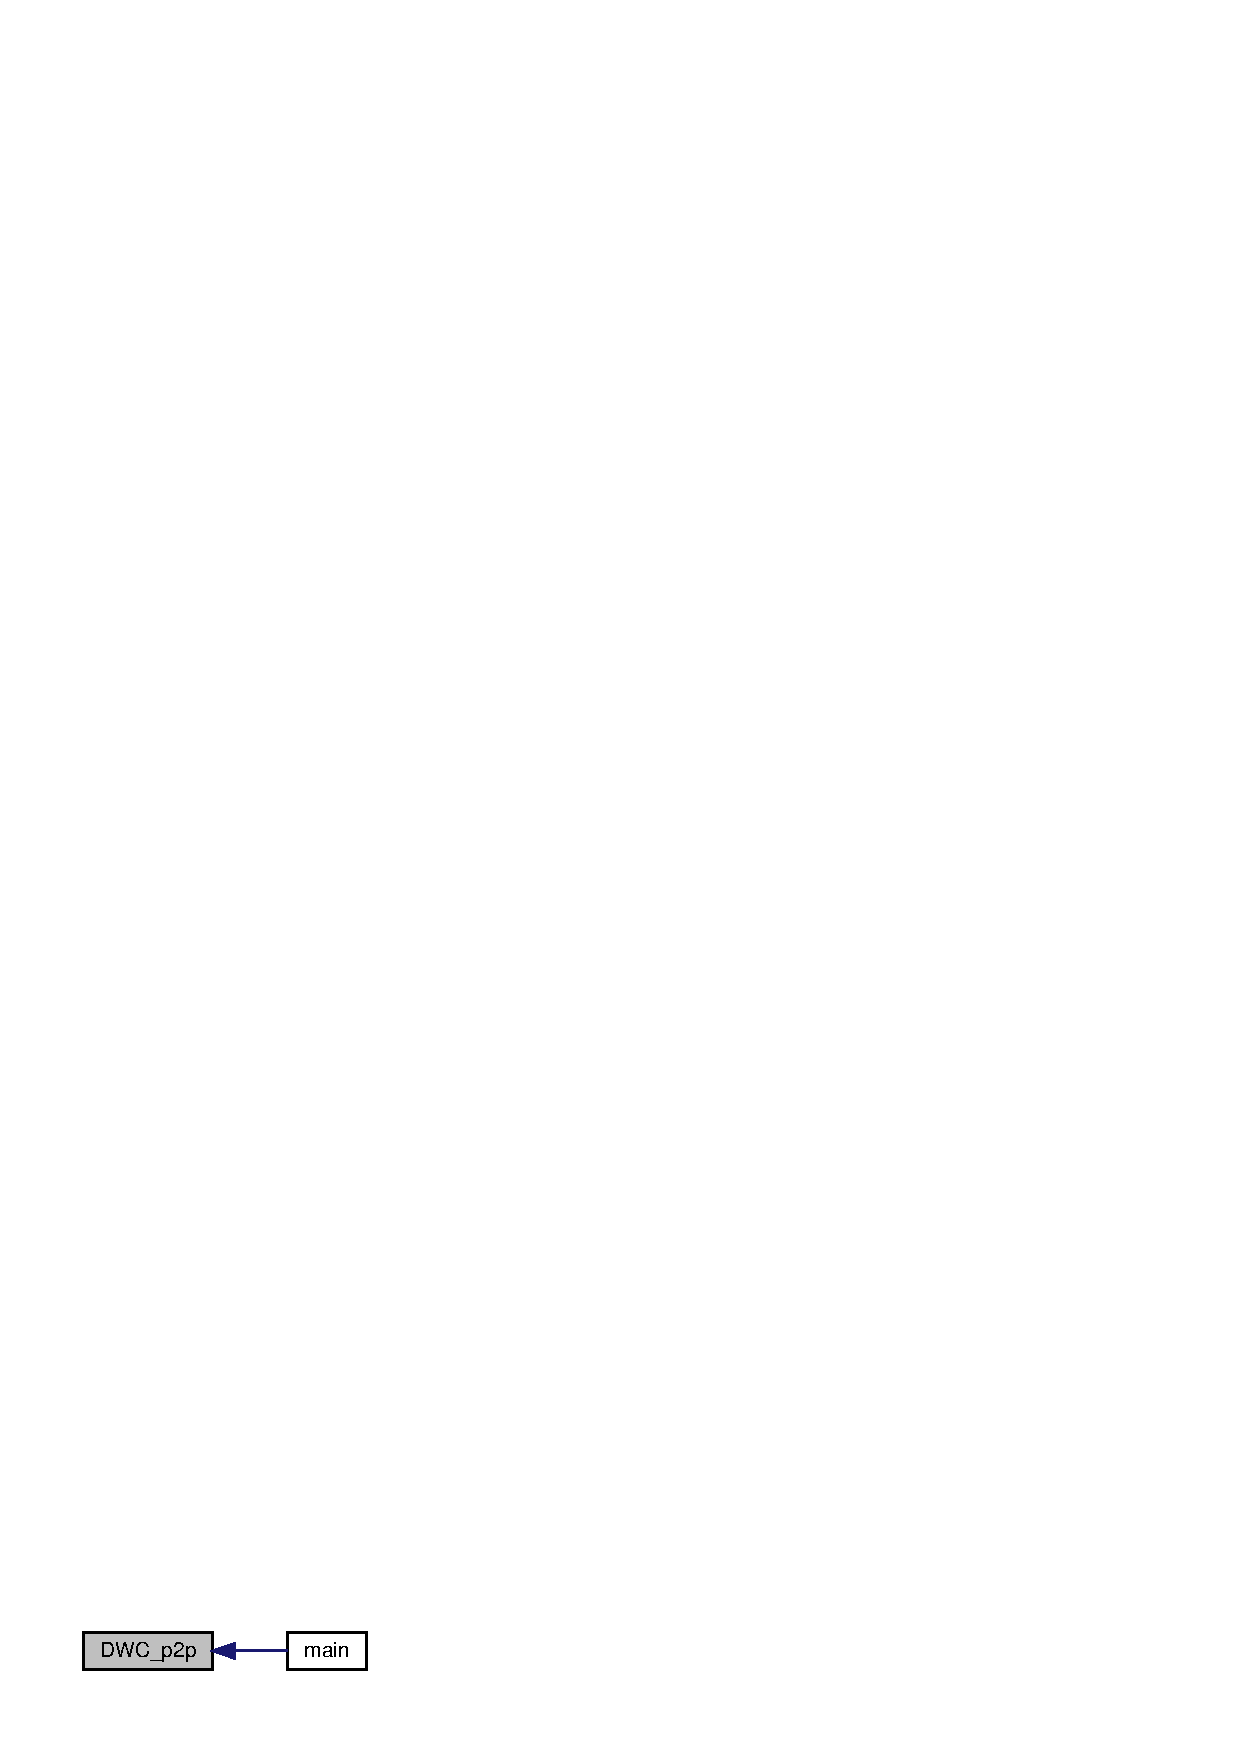
\includegraphics[width=180pt]{Conti2D_8cpp_ab87ce573de93575b7ece2e4f772e03fd_ab87ce573de93575b7ece2e4f772e03fd_icgraph}
\end{center}
\end{figure}
\mbox{\label{Conti2D_8cpp_a68e9e4a8817a29dce16c782fa8213faa_a68e9e4a8817a29dce16c782fa8213faa}} 
\index{Conti2\+D.\+cpp@{Conti2\+D.\+cpp}!D\+W\+C\+\_\+p2p\+\_\+\+C\+G\+LS@{D\+W\+C\+\_\+p2p\+\_\+\+C\+G\+LS}}
\index{D\+W\+C\+\_\+p2p\+\_\+\+C\+G\+LS@{D\+W\+C\+\_\+p2p\+\_\+\+C\+G\+LS}!Conti2\+D.\+cpp@{Conti2\+D.\+cpp}}
\subsubsection{D\+W\+C\+\_\+p2p\+\_\+\+C\+G\+L\+S()}
{\footnotesize\ttfamily void D\+W\+C\+\_\+p2p\+\_\+\+C\+G\+LS (\begin{DoxyParamCaption}\item[{double $\ast$}]{G\+\_\+first\+Row,  }\item[{double $\ast$}]{x,  }\item[{double $\ast$}]{b,  }\item[{\textbf{ Grd\+Head}}]{grdhead,  }\item[{int}]{ext\+Num,  }\item[{double}]{delta,  }\item[{int}]{num\+\_\+thread }\end{DoxyParamCaption})}



Definition at line 1402 of file Conti2\+D.\+cpp.



References Grd\+Head\+::cols, Norm2(), Grd\+Head\+::rows, Save\+Grd(), Multi\+Progress\+Bar\+::\+Update(), U\+W\+C\+\_\+\+Gij(), and U\+W\+C\+\_\+\+Gji().

Here is the call graph for this function\+:
\nopagebreak
\begin{figure}[H]
\begin{center}
\leavevmode
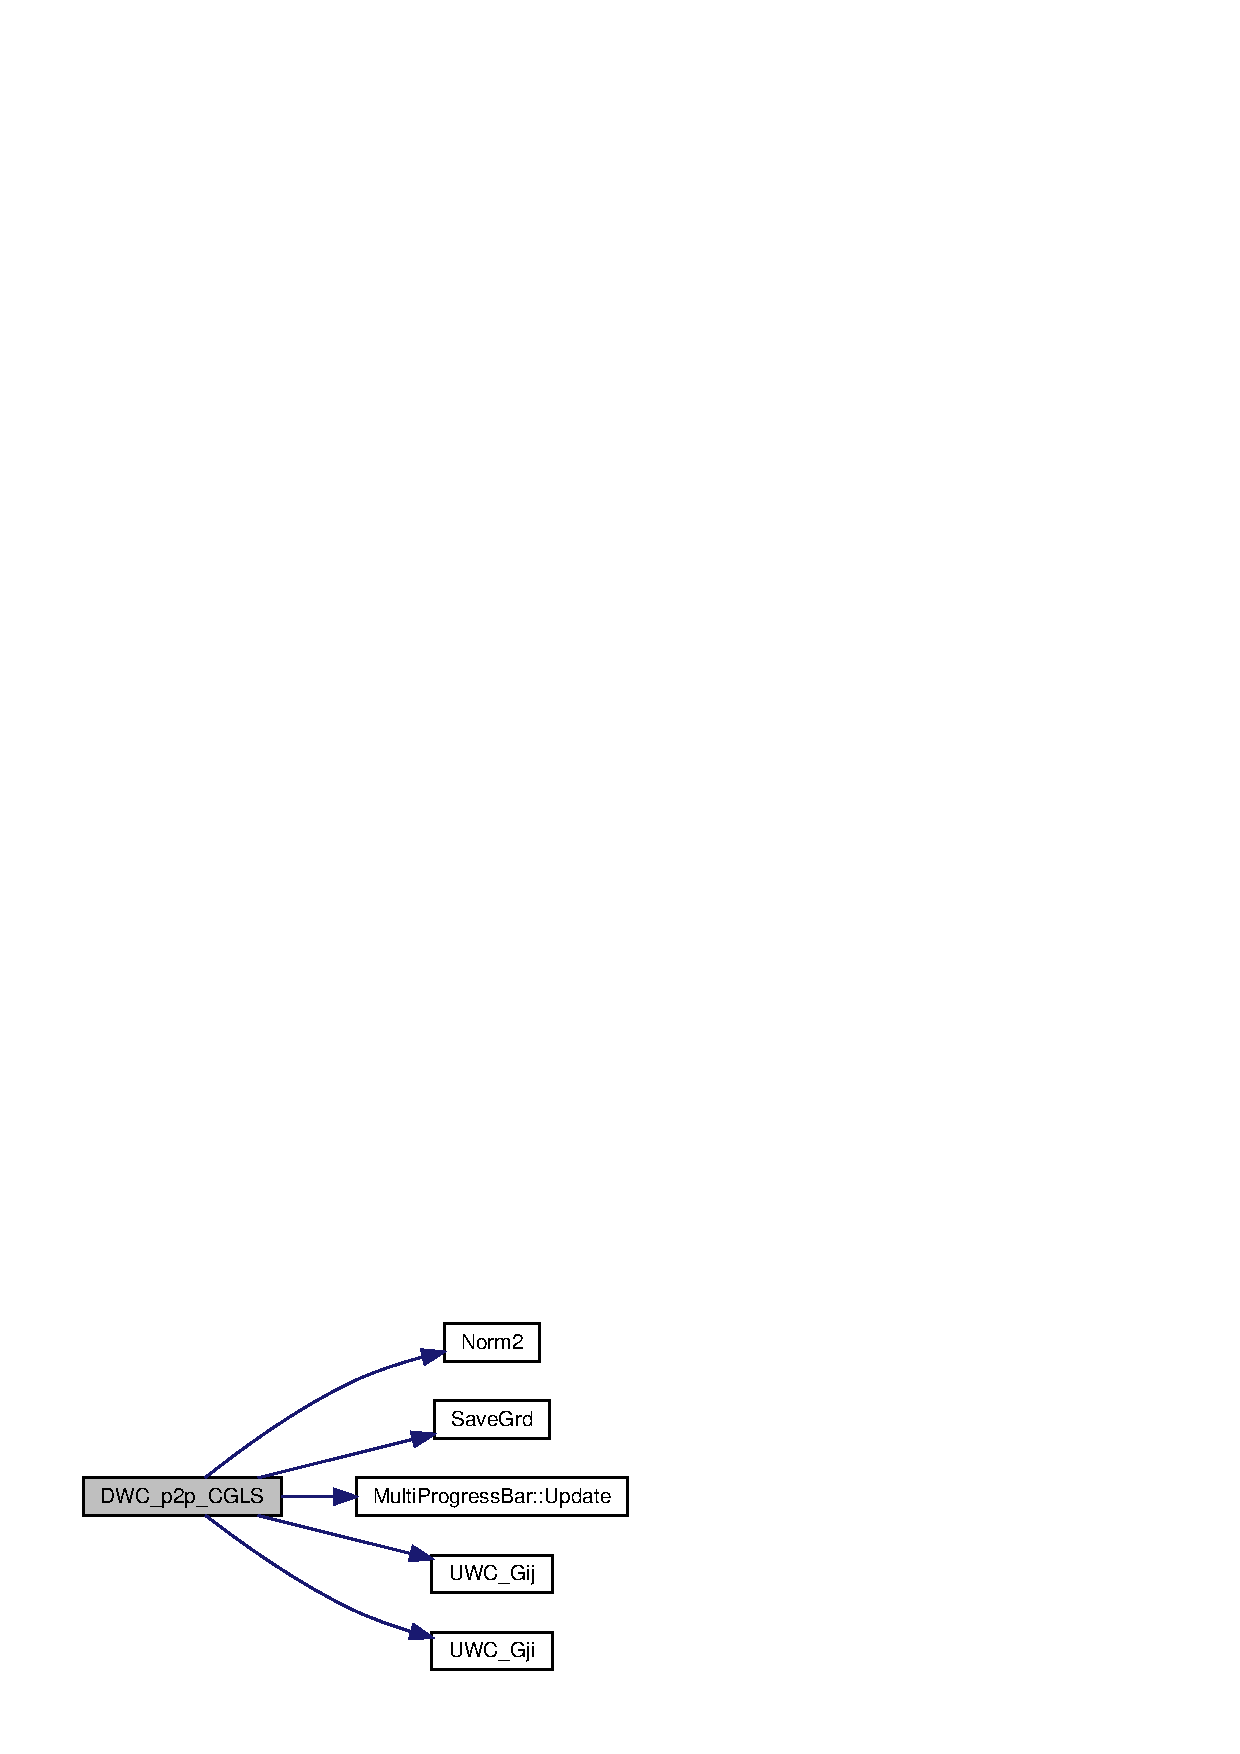
\includegraphics[width=305pt]{Conti2D_8cpp_a68e9e4a8817a29dce16c782fa8213faa_a68e9e4a8817a29dce16c782fa8213faa_cgraph}
\end{center}
\end{figure}
\mbox{\label{Conti2D_8cpp_afb187c363388d28caa8a055176269f12_afb187c363388d28caa8a055176269f12}} 
\index{Conti2\+D.\+cpp@{Conti2\+D.\+cpp}!D\+W\+C\+\_\+p2p\+\_\+f@{D\+W\+C\+\_\+p2p\+\_\+f}}
\index{D\+W\+C\+\_\+p2p\+\_\+f@{D\+W\+C\+\_\+p2p\+\_\+f}!Conti2\+D.\+cpp@{Conti2\+D.\+cpp}}
\subsubsection{D\+W\+C\+\_\+p2p\+\_\+f()}
{\footnotesize\ttfamily void D\+W\+C\+\_\+p2p\+\_\+f (\begin{DoxyParamCaption}\item[{string}]{inputfilename,  }\item[{string}]{outputfilename,  }\item[{double}]{height1,  }\item[{double}]{height2,  }\item[{int}]{ext\+Num,  }\item[{double}]{T\+RP,  }\item[{int}]{num\+\_\+thread,  }\item[{bool}]{is\+Progress,  }\item[{bool}]{use\+Old\+Kernel }\end{DoxyParamCaption})}



Definition at line 976 of file Conti2\+D.\+cpp.



References Grd\+Head\+::bounds, Grd\+Head\+::cols, Get\+Kernal\+Matrix\+\_\+new(), Read\+Grd(), Grd\+Head\+::rows, Save\+Grd(), and U\+W\+C\+\_\+p2p\+\_\+f().



Referenced by main().

Here is the call graph for this function\+:
\nopagebreak
\begin{figure}[H]
\begin{center}
\leavevmode
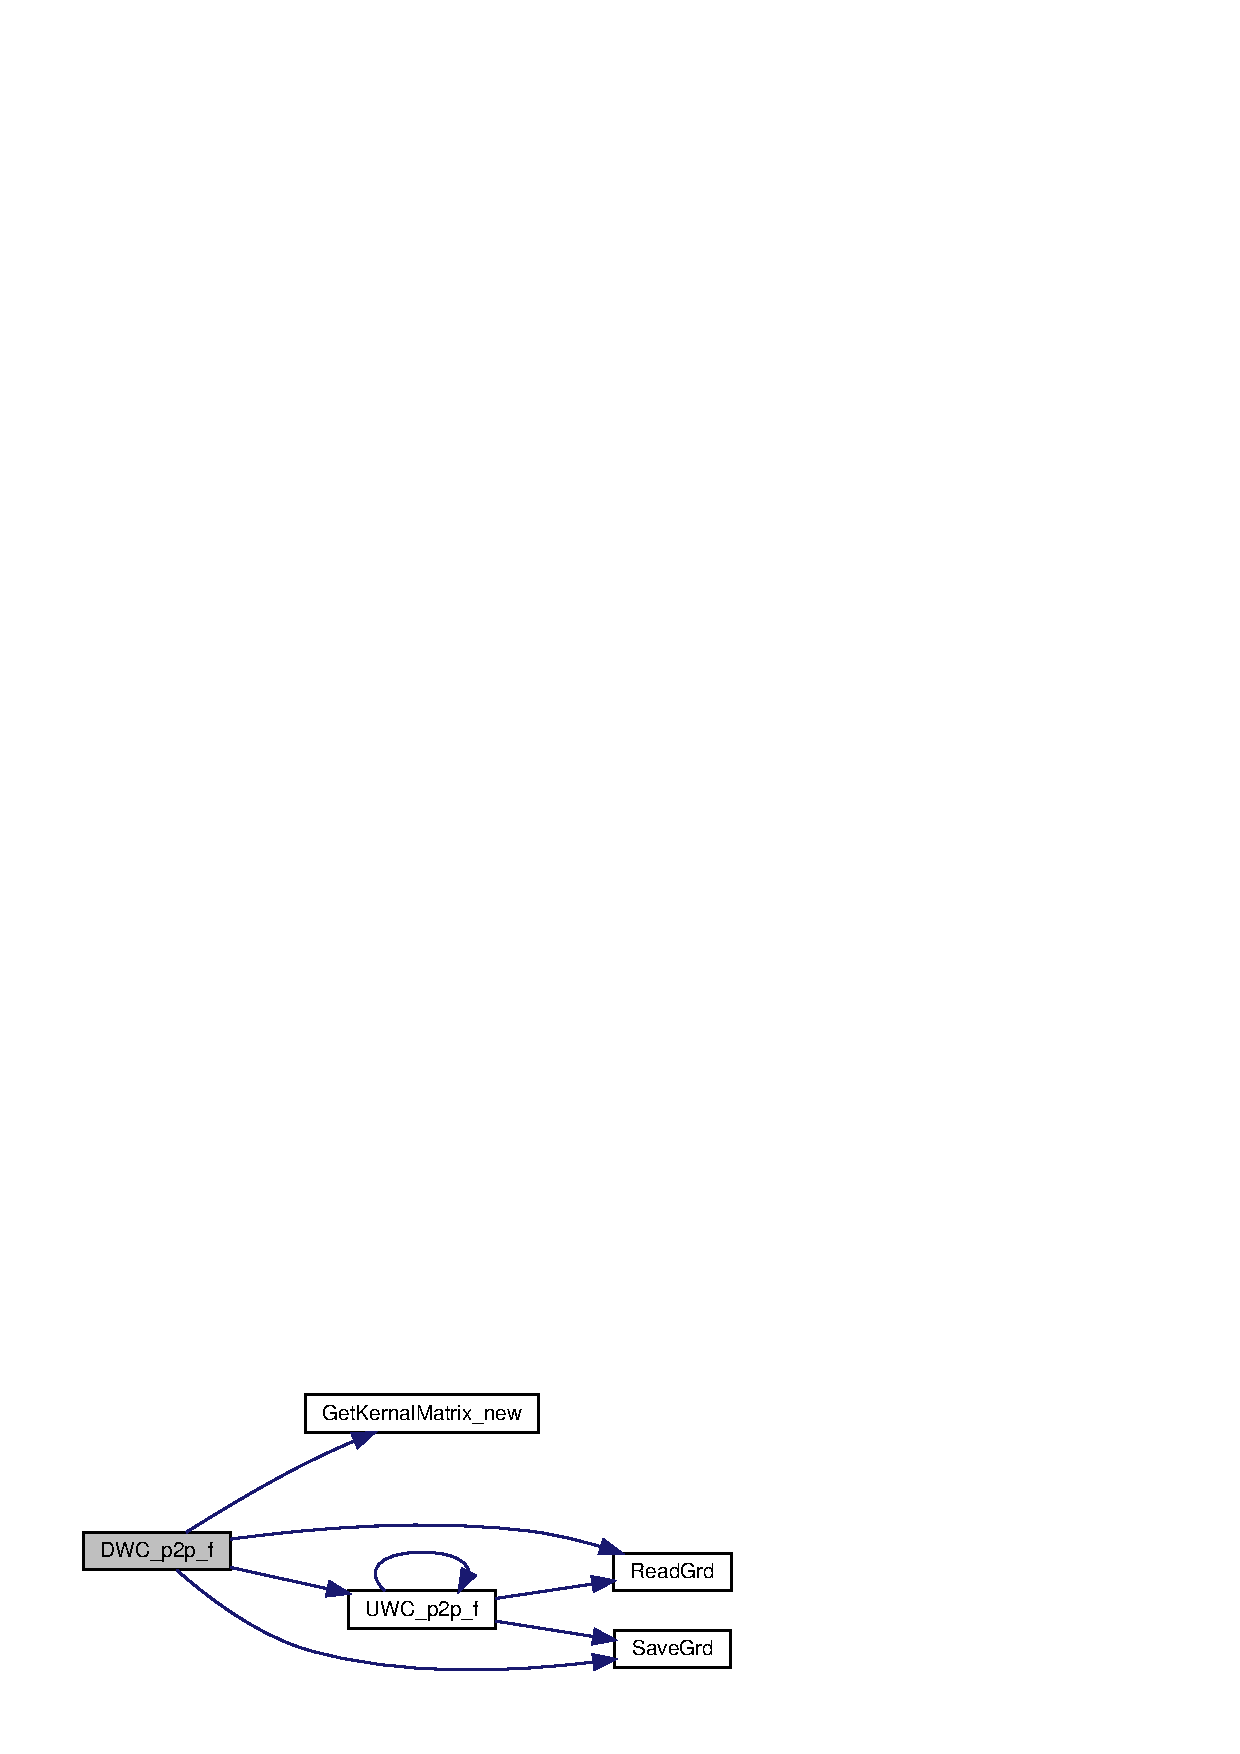
\includegraphics[width=350pt]{Conti2D_8cpp_afb187c363388d28caa8a055176269f12_afb187c363388d28caa8a055176269f12_cgraph}
\end{center}
\end{figure}
Here is the caller graph for this function\+:\nopagebreak
\begin{figure}[H]
\begin{center}
\leavevmode
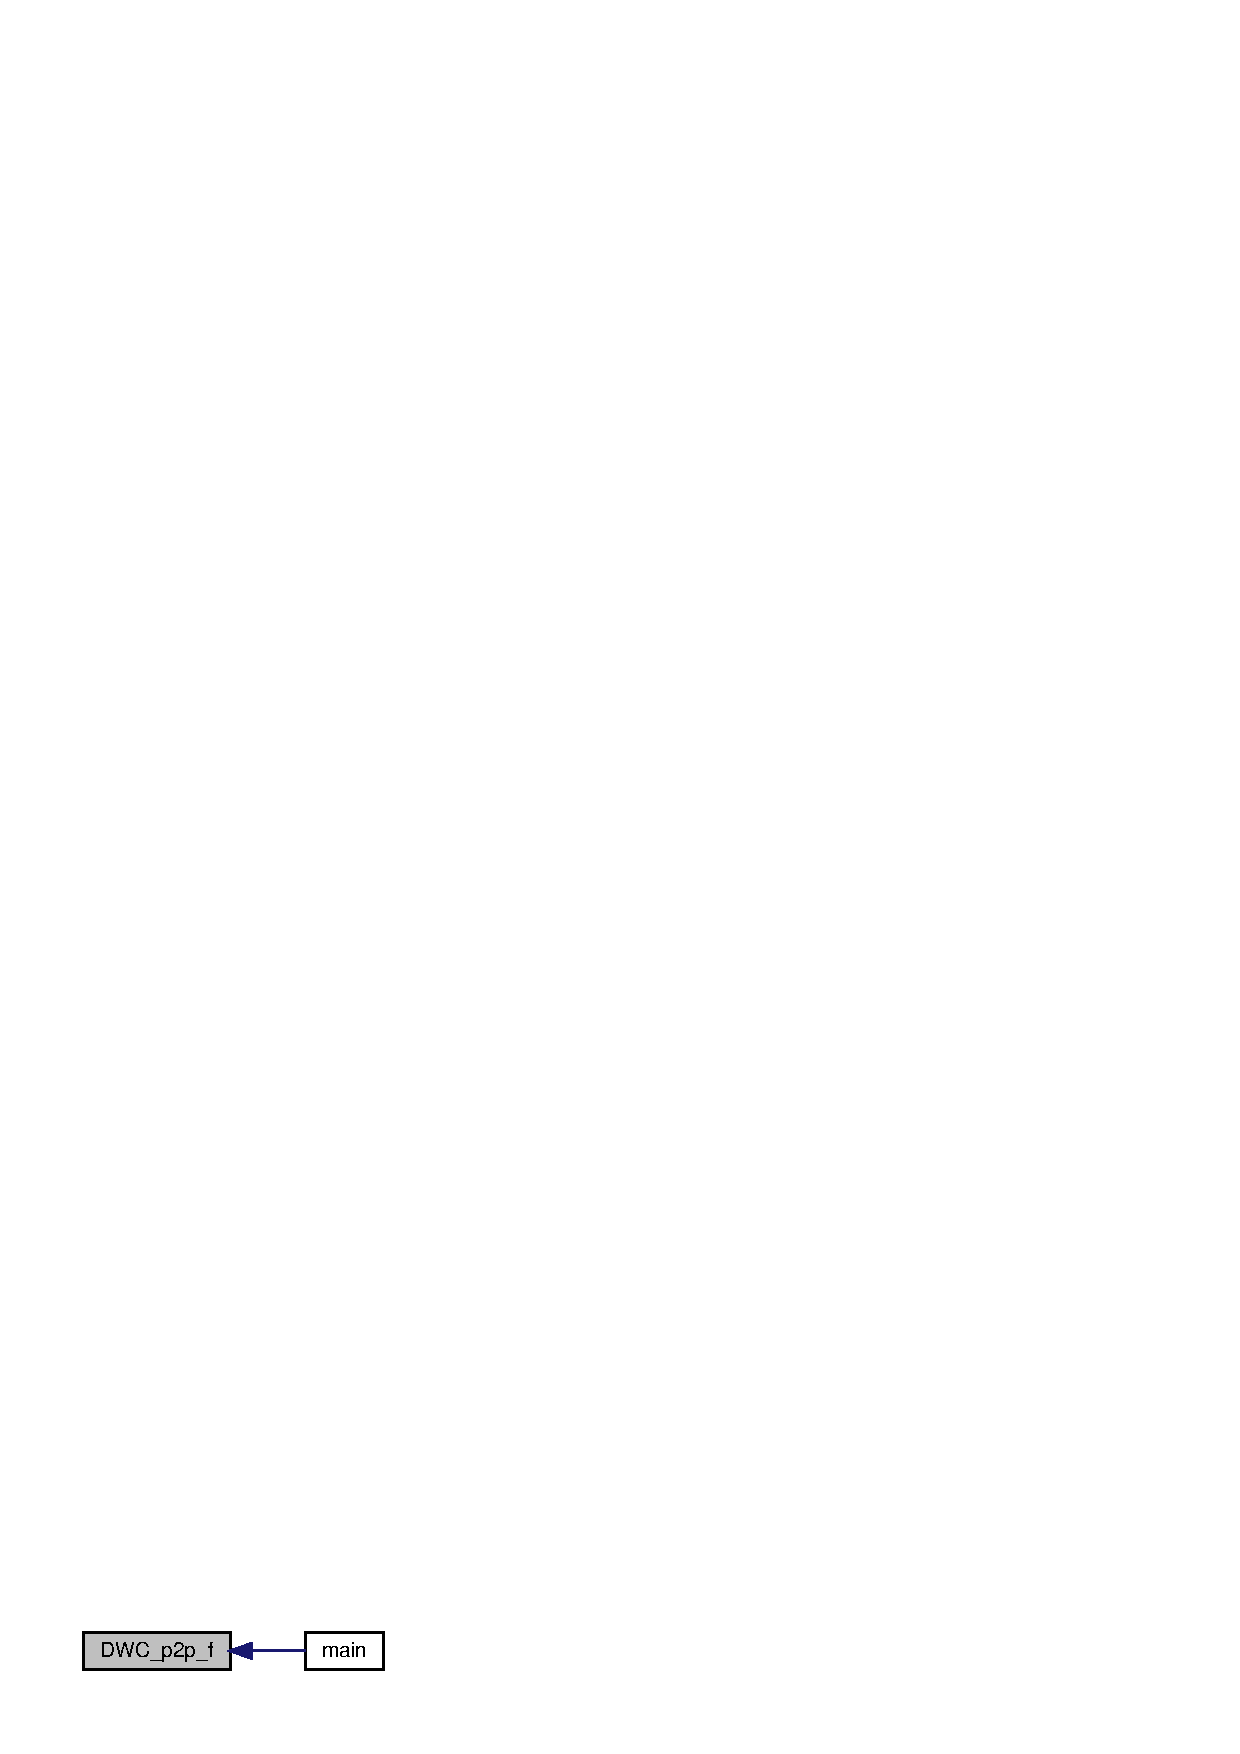
\includegraphics[width=188pt]{Conti2D_8cpp_afb187c363388d28caa8a055176269f12_afb187c363388d28caa8a055176269f12_icgraph}
\end{center}
\end{figure}
\mbox{\label{Conti2D_8cpp_ad9d4ab56b3ff557565d82cf01ab598ad_ad9d4ab56b3ff557565d82cf01ab598ad}} 
\index{Conti2\+D.\+cpp@{Conti2\+D.\+cpp}!D\+W\+C\+\_\+p2p\+\_\+\+Itegration\+Iter@{D\+W\+C\+\_\+p2p\+\_\+\+Itegration\+Iter}}
\index{D\+W\+C\+\_\+p2p\+\_\+\+Itegration\+Iter@{D\+W\+C\+\_\+p2p\+\_\+\+Itegration\+Iter}!Conti2\+D.\+cpp@{Conti2\+D.\+cpp}}
\subsubsection{D\+W\+C\+\_\+p2p\+\_\+\+Itegration\+Iter()}
{\footnotesize\ttfamily void D\+W\+C\+\_\+p2p\+\_\+\+Itegration\+Iter (\begin{DoxyParamCaption}\item[{double $\ast$}]{G,  }\item[{double $\ast$}]{x,  }\item[{double $\ast$}]{b,  }\item[{\textbf{ Grd\+Head}}]{grdhead,  }\item[{int}]{ext\+Num,  }\item[{int}]{num\+\_\+thread,  }\item[{string}]{outputfile,  }\item[{double}]{iter\+\_\+number,  }\item[{double $\ast$}]{Exact\+Solution }\end{DoxyParamCaption})}



Definition at line 1768 of file Conti2\+D.\+cpp.



References C\+O\+L\+O\+R\+\_\+\+D\+E\+F\+A\+L\+UT, Grd\+Head\+::cols, G\+R\+E\+EN, Norm2(), Norm2\+\_\+\+Gradient(), Path\+\_\+\+Get\+File\+Name(), R\+ED, Grd\+Head\+::rows, Save\+Grd(), Multi\+Progress\+Bar\+::\+Update(), and U\+W\+C\+\_\+\+Gij().

Here is the call graph for this function\+:
\nopagebreak
\begin{figure}[H]
\begin{center}
\leavevmode
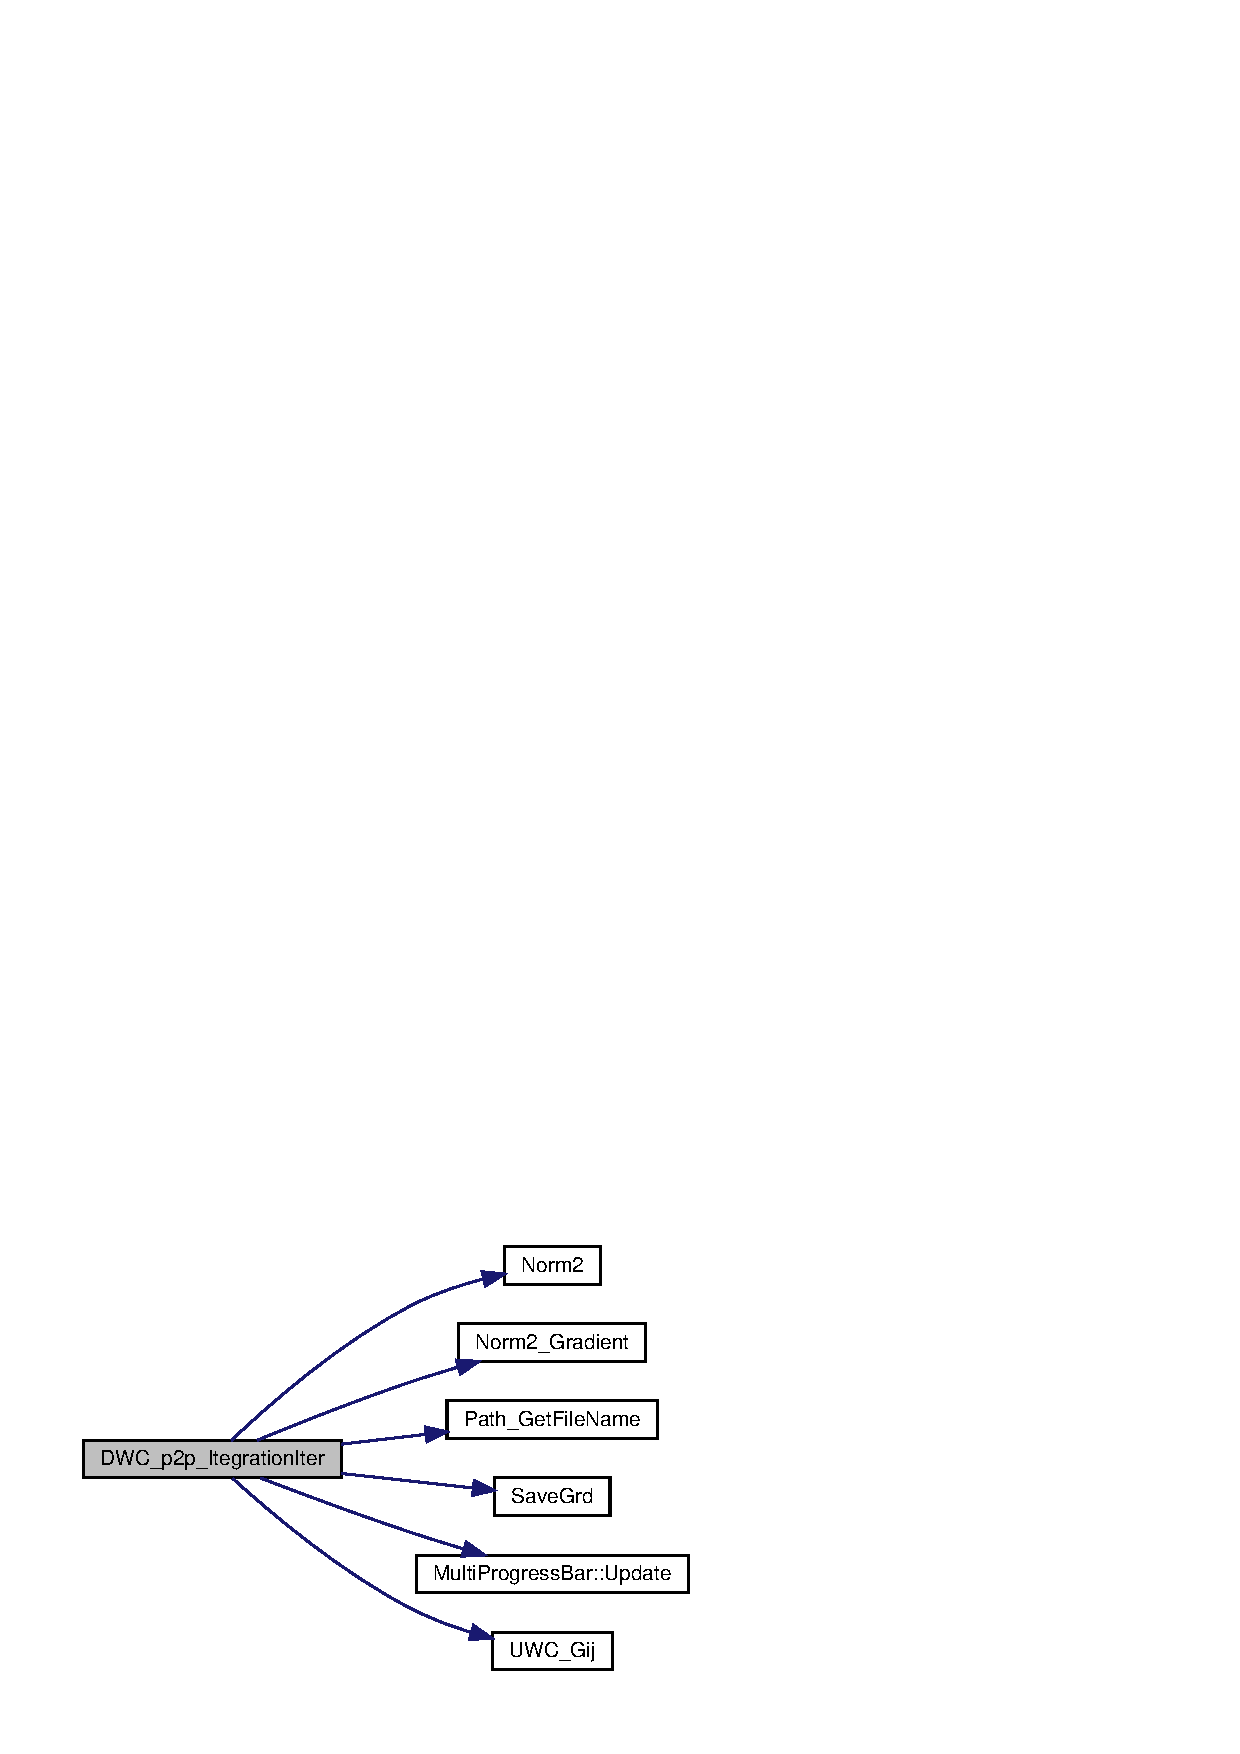
\includegraphics[width=334pt]{Conti2D_8cpp_ad9d4ab56b3ff557565d82cf01ab598ad_ad9d4ab56b3ff557565d82cf01ab598ad_cgraph}
\end{center}
\end{figure}
\mbox{\label{Conti2D_8cpp_a9a4db1b002682739ba7b888c536da886_a9a4db1b002682739ba7b888c536da886}} 
\index{Conti2\+D.\+cpp@{Conti2\+D.\+cpp}!D\+W\+C\+\_\+p2p\+\_\+\+Landweber\+Iter@{D\+W\+C\+\_\+p2p\+\_\+\+Landweber\+Iter}}
\index{D\+W\+C\+\_\+p2p\+\_\+\+Landweber\+Iter@{D\+W\+C\+\_\+p2p\+\_\+\+Landweber\+Iter}!Conti2\+D.\+cpp@{Conti2\+D.\+cpp}}
\subsubsection{D\+W\+C\+\_\+p2p\+\_\+\+Landweber\+Iter()}
{\footnotesize\ttfamily void D\+W\+C\+\_\+p2p\+\_\+\+Landweber\+Iter (\begin{DoxyParamCaption}\item[{double $\ast$}]{G,  }\item[{double $\ast$}]{x,  }\item[{double $\ast$}]{b,  }\item[{\textbf{ Grd\+Head}}]{grdhead,  }\item[{int}]{ext\+Num,  }\item[{int}]{num\+\_\+thread,  }\item[{string}]{outputfile,  }\item[{double}]{iter\+\_\+number,  }\item[{double $\ast$}]{Exact\+Solution }\end{DoxyParamCaption})}



Definition at line 1848 of file Conti2\+D.\+cpp.



References C\+O\+L\+O\+R\+\_\+\+D\+E\+F\+A\+L\+UT, Grd\+Head\+::cols, G\+R\+E\+EN, Norm2(), Norm2\+\_\+\+Gradient(), Path\+\_\+\+Get\+File\+Name(), R\+ED, Grd\+Head\+::rows, Save\+Grd(), Multi\+Progress\+Bar\+::\+Update(), and U\+W\+C\+\_\+\+Gij().

Here is the call graph for this function\+:
\nopagebreak
\begin{figure}[H]
\begin{center}
\leavevmode
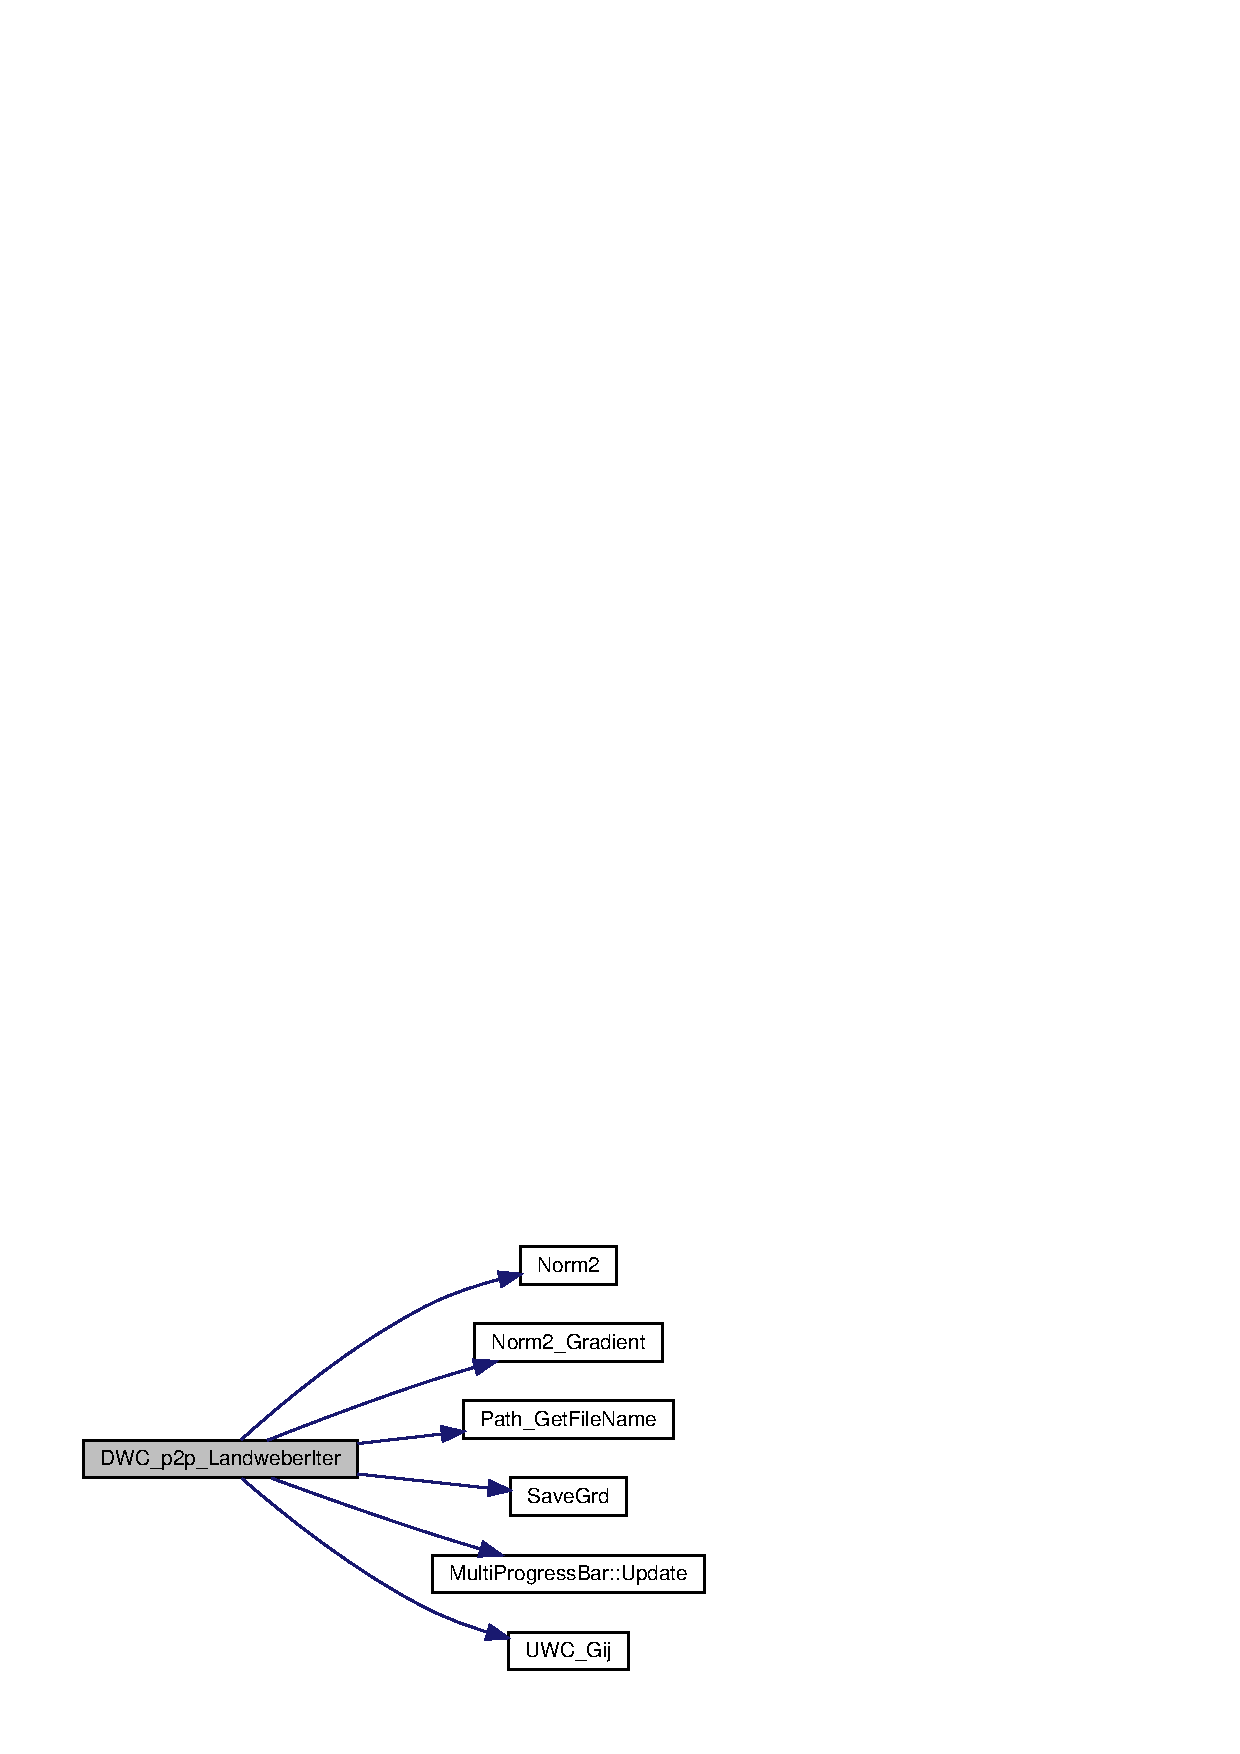
\includegraphics[width=342pt]{Conti2D_8cpp_a9a4db1b002682739ba7b888c536da886_a9a4db1b002682739ba7b888c536da886_cgraph}
\end{center}
\end{figure}
\mbox{\label{Conti2D_8cpp_ab256354d6264edd8deb4e31f98a7489f_ab256354d6264edd8deb4e31f98a7489f}} 
\index{Conti2\+D.\+cpp@{Conti2\+D.\+cpp}!D\+W\+C\+\_\+s2p@{D\+W\+C\+\_\+s2p}}
\index{D\+W\+C\+\_\+s2p@{D\+W\+C\+\_\+s2p}!Conti2\+D.\+cpp@{Conti2\+D.\+cpp}}
\subsubsection{D\+W\+C\+\_\+s2p()}
{\footnotesize\ttfamily void D\+W\+C\+\_\+s2p (\begin{DoxyParamCaption}\item[{string}]{inputfilename,  }\item[{string}]{outputfilename,  }\item[{string}]{topo\+File,  }\item[{double}]{height2,  }\item[{int}]{ext\+Num,  }\item[{double}]{D\+W\+C\+\_\+parameter,  }\item[{int}]{D\+W\+C\+\_\+method,  }\item[{int}]{num\+\_\+thread,  }\item[{bool}]{is\+Progress,  }\item[{bool}]{use\+Old\+Kernel,  }\item[{string}]{filename\+\_\+exact }\end{DoxyParamCaption})}



Definition at line 1203 of file Conti2\+D.\+cpp.



References Grd\+Head\+::bounds, C\+O\+L\+O\+R\+\_\+\+D\+E\+F\+A\+L\+UT, Grd\+Head\+::cols, D\+W\+C\+\_\+\+C\+G\+LS, D\+W\+C\+\_\+\+I\+N\+T\+E\+G\+R\+A\+L\+I\+T\+E\+R\+A\+T\+I\+ON, D\+W\+C\+\_\+\+L\+A\+N\+D\+W\+E\+B\+ER, D\+W\+C\+\_\+s2p\+\_\+\+C\+G\+L\+S(), D\+W\+C\+\_\+s2p\+\_\+\+Itegration\+Iter(), D\+W\+C\+\_\+s2p\+\_\+\+Landweber\+Iter(), D\+W\+C\+\_\+\+T\+I\+K\+H\+O\+N\+OV, Getkernel\+\_\+p2s\+\_\+new(), Read\+Grd(), R\+ED, Grd\+Head\+::rows, and Save\+Grd().



Referenced by main().

Here is the call graph for this function\+:
\nopagebreak
\begin{figure}[H]
\begin{center}
\leavevmode
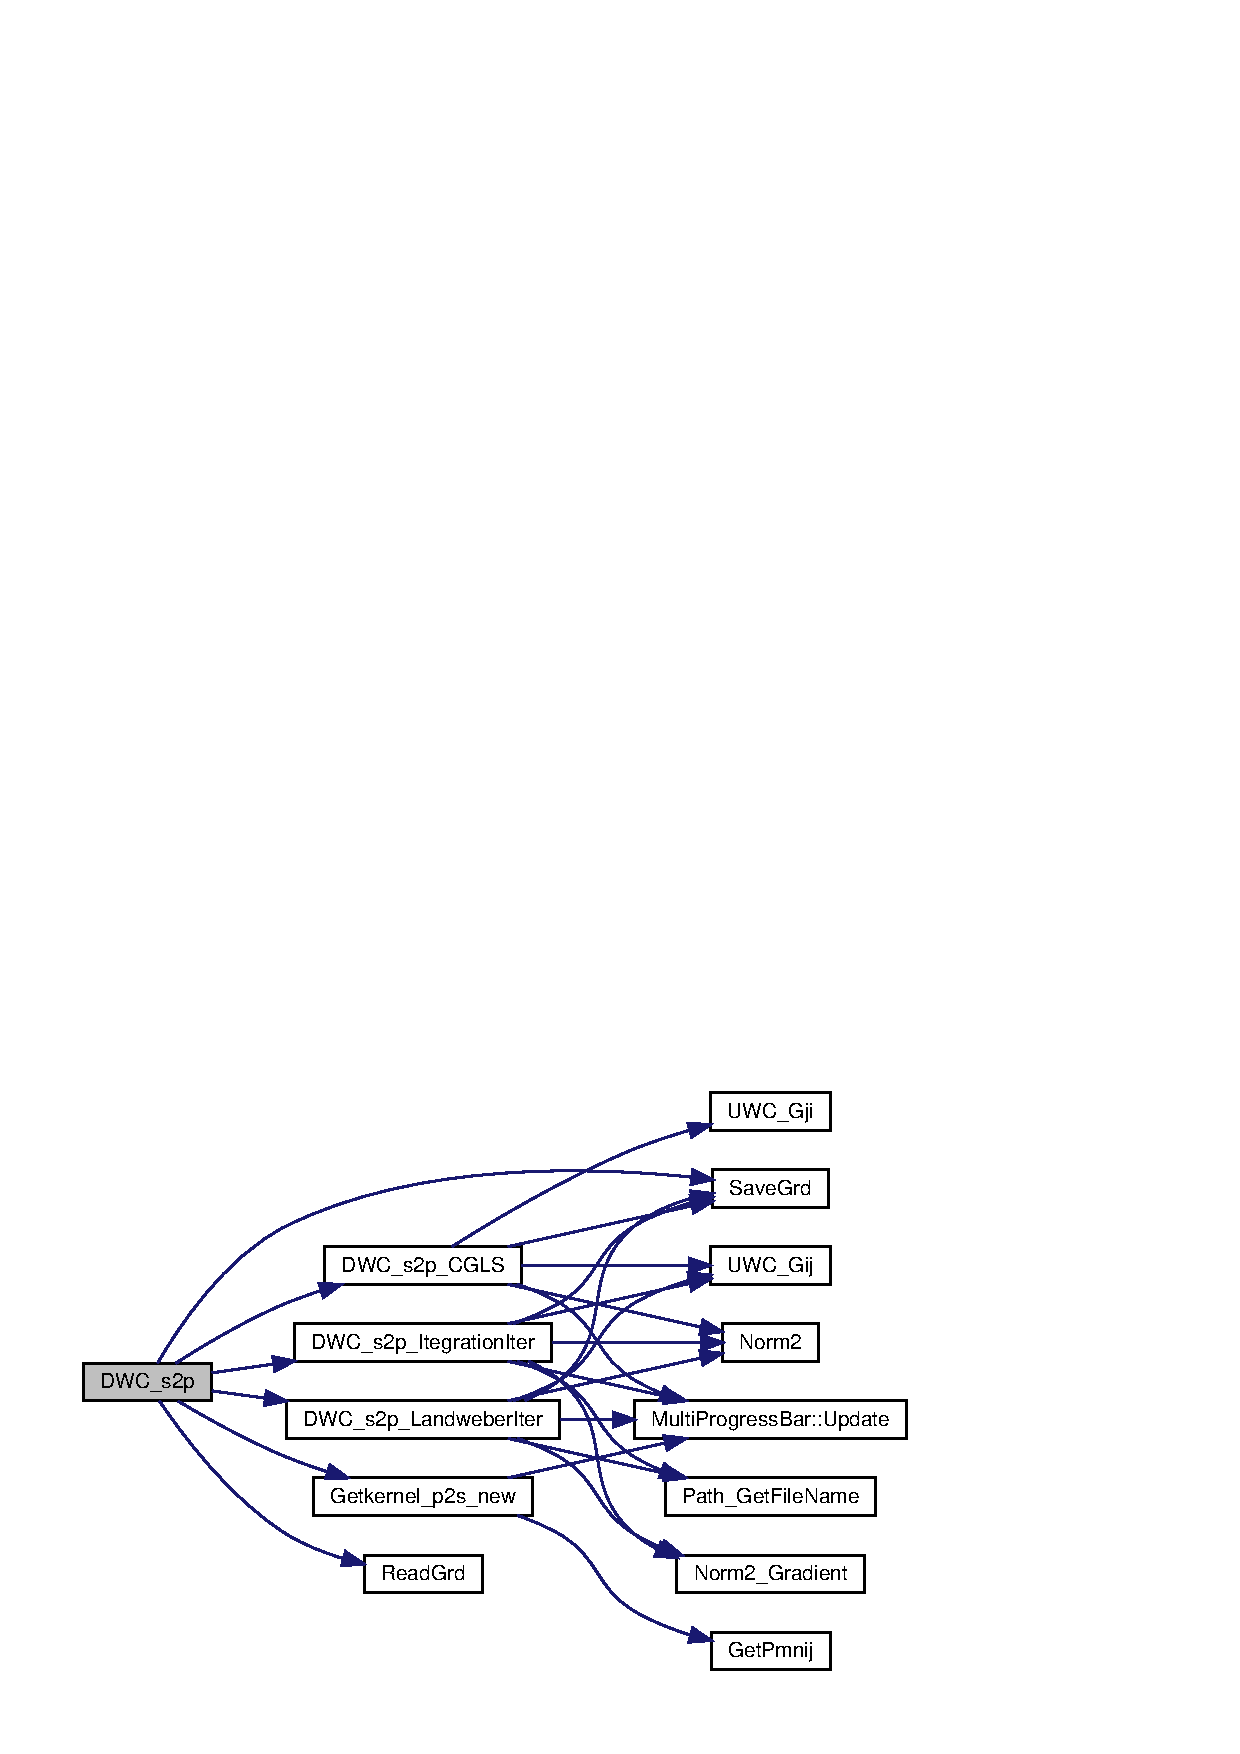
\includegraphics[width=350pt]{Conti2D_8cpp_ab256354d6264edd8deb4e31f98a7489f_ab256354d6264edd8deb4e31f98a7489f_cgraph}
\end{center}
\end{figure}
Here is the caller graph for this function\+:\nopagebreak
\begin{figure}[H]
\begin{center}
\leavevmode
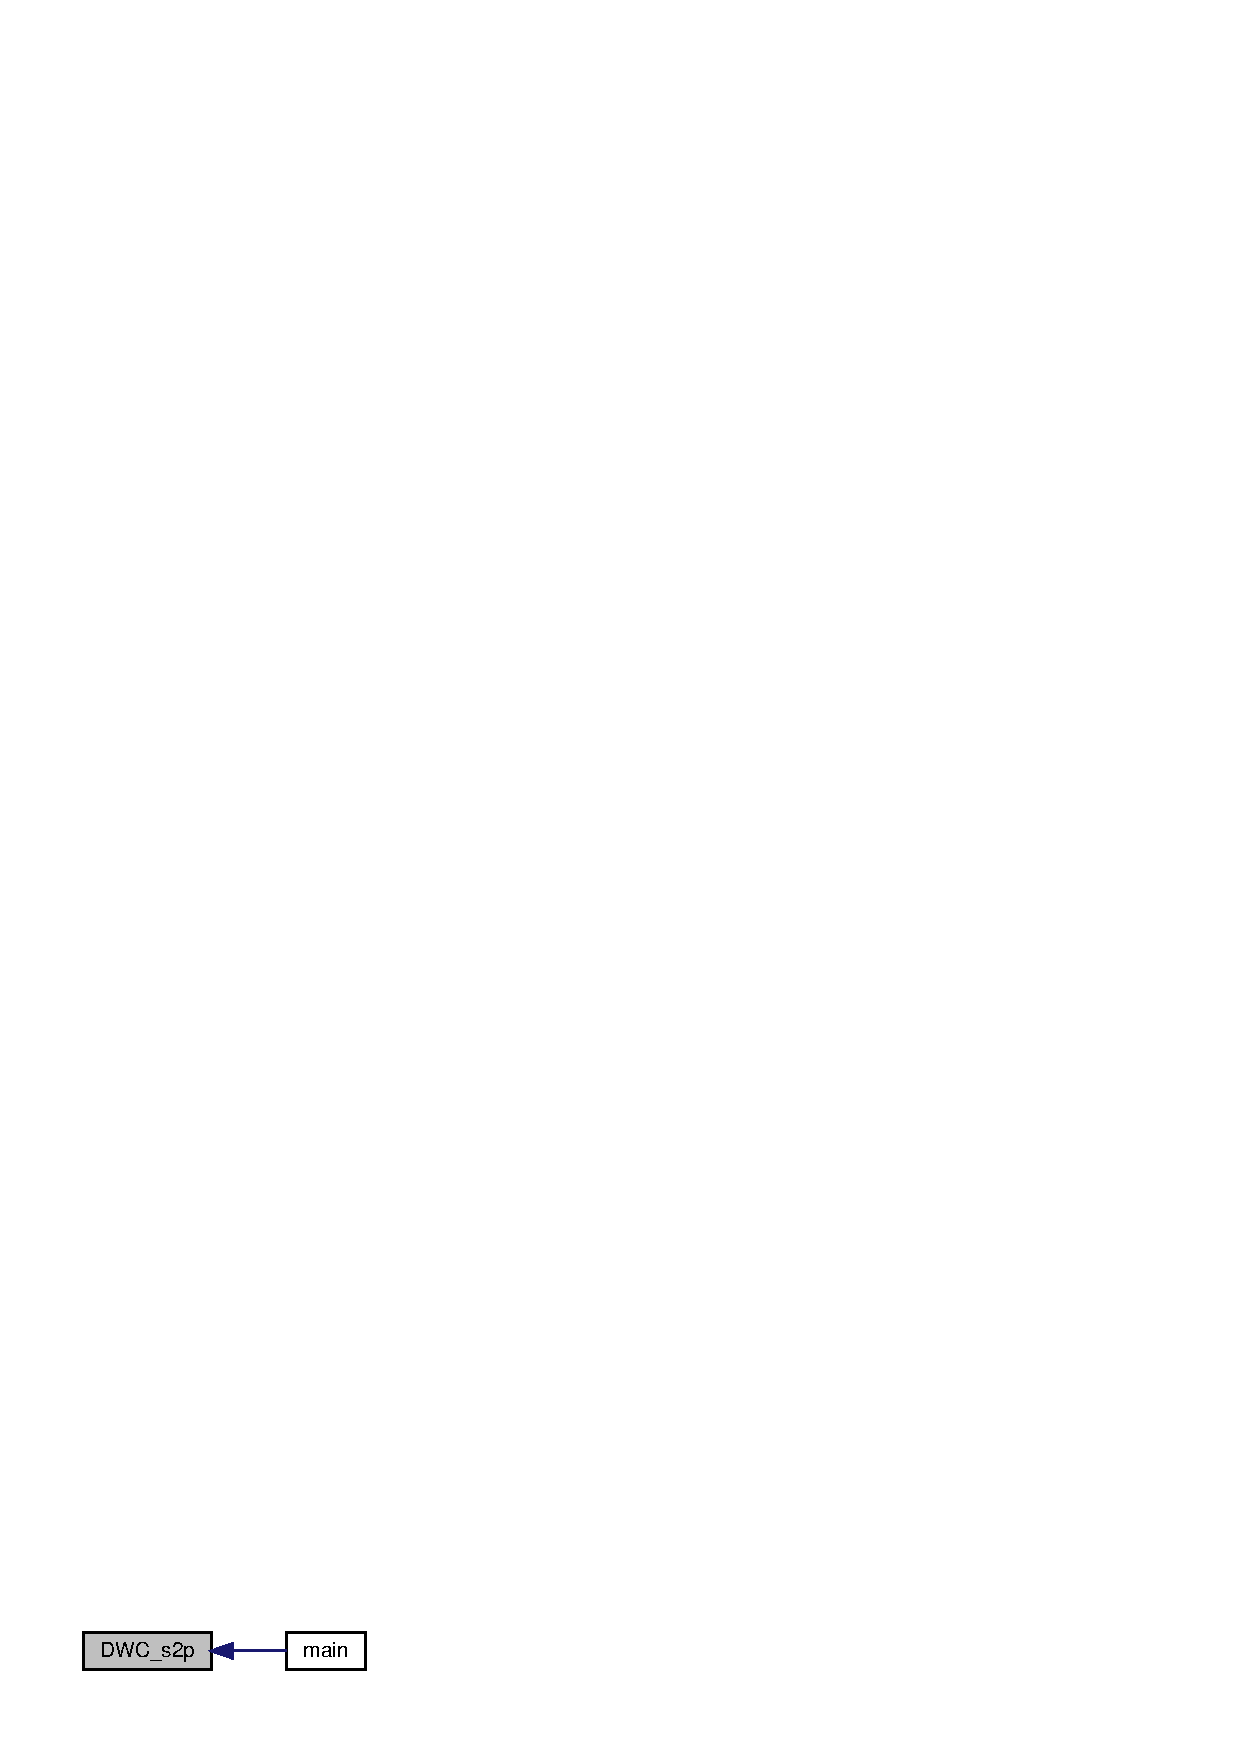
\includegraphics[width=179pt]{Conti2D_8cpp_ab256354d6264edd8deb4e31f98a7489f_ab256354d6264edd8deb4e31f98a7489f_icgraph}
\end{center}
\end{figure}
\mbox{\label{Conti2D_8cpp_a6516cfeb71abcf844b32f101e5f77a71_a6516cfeb71abcf844b32f101e5f77a71}} 
\index{Conti2\+D.\+cpp@{Conti2\+D.\+cpp}!D\+W\+C\+\_\+s2p\+\_\+\+C\+G\+LS@{D\+W\+C\+\_\+s2p\+\_\+\+C\+G\+LS}}
\index{D\+W\+C\+\_\+s2p\+\_\+\+C\+G\+LS@{D\+W\+C\+\_\+s2p\+\_\+\+C\+G\+LS}!Conti2\+D.\+cpp@{Conti2\+D.\+cpp}}
\subsubsection{D\+W\+C\+\_\+s2p\+\_\+\+C\+G\+L\+S()}
{\footnotesize\ttfamily void D\+W\+C\+\_\+s2p\+\_\+\+C\+G\+LS (\begin{DoxyParamCaption}\item[{double $\ast$$\ast$}]{G,  }\item[{double $\ast$}]{x,  }\item[{double $\ast$}]{b,  }\item[{\textbf{ Grd\+Head}}]{grdhead,  }\item[{int}]{ext\+Num,  }\item[{double}]{delta,  }\item[{int}]{num\+\_\+thread }\end{DoxyParamCaption})}



Definition at line 1488 of file Conti2\+D.\+cpp.



References Grd\+Head\+::cols, Norm2(), Grd\+Head\+::rows, Save\+Grd(), Multi\+Progress\+Bar\+::\+Update(), U\+W\+C\+\_\+\+Gij(), and U\+W\+C\+\_\+\+Gji().



Referenced by D\+W\+C\+\_\+p2p(), and D\+W\+C\+\_\+s2p().

Here is the call graph for this function\+:
\nopagebreak
\begin{figure}[H]
\begin{center}
\leavevmode
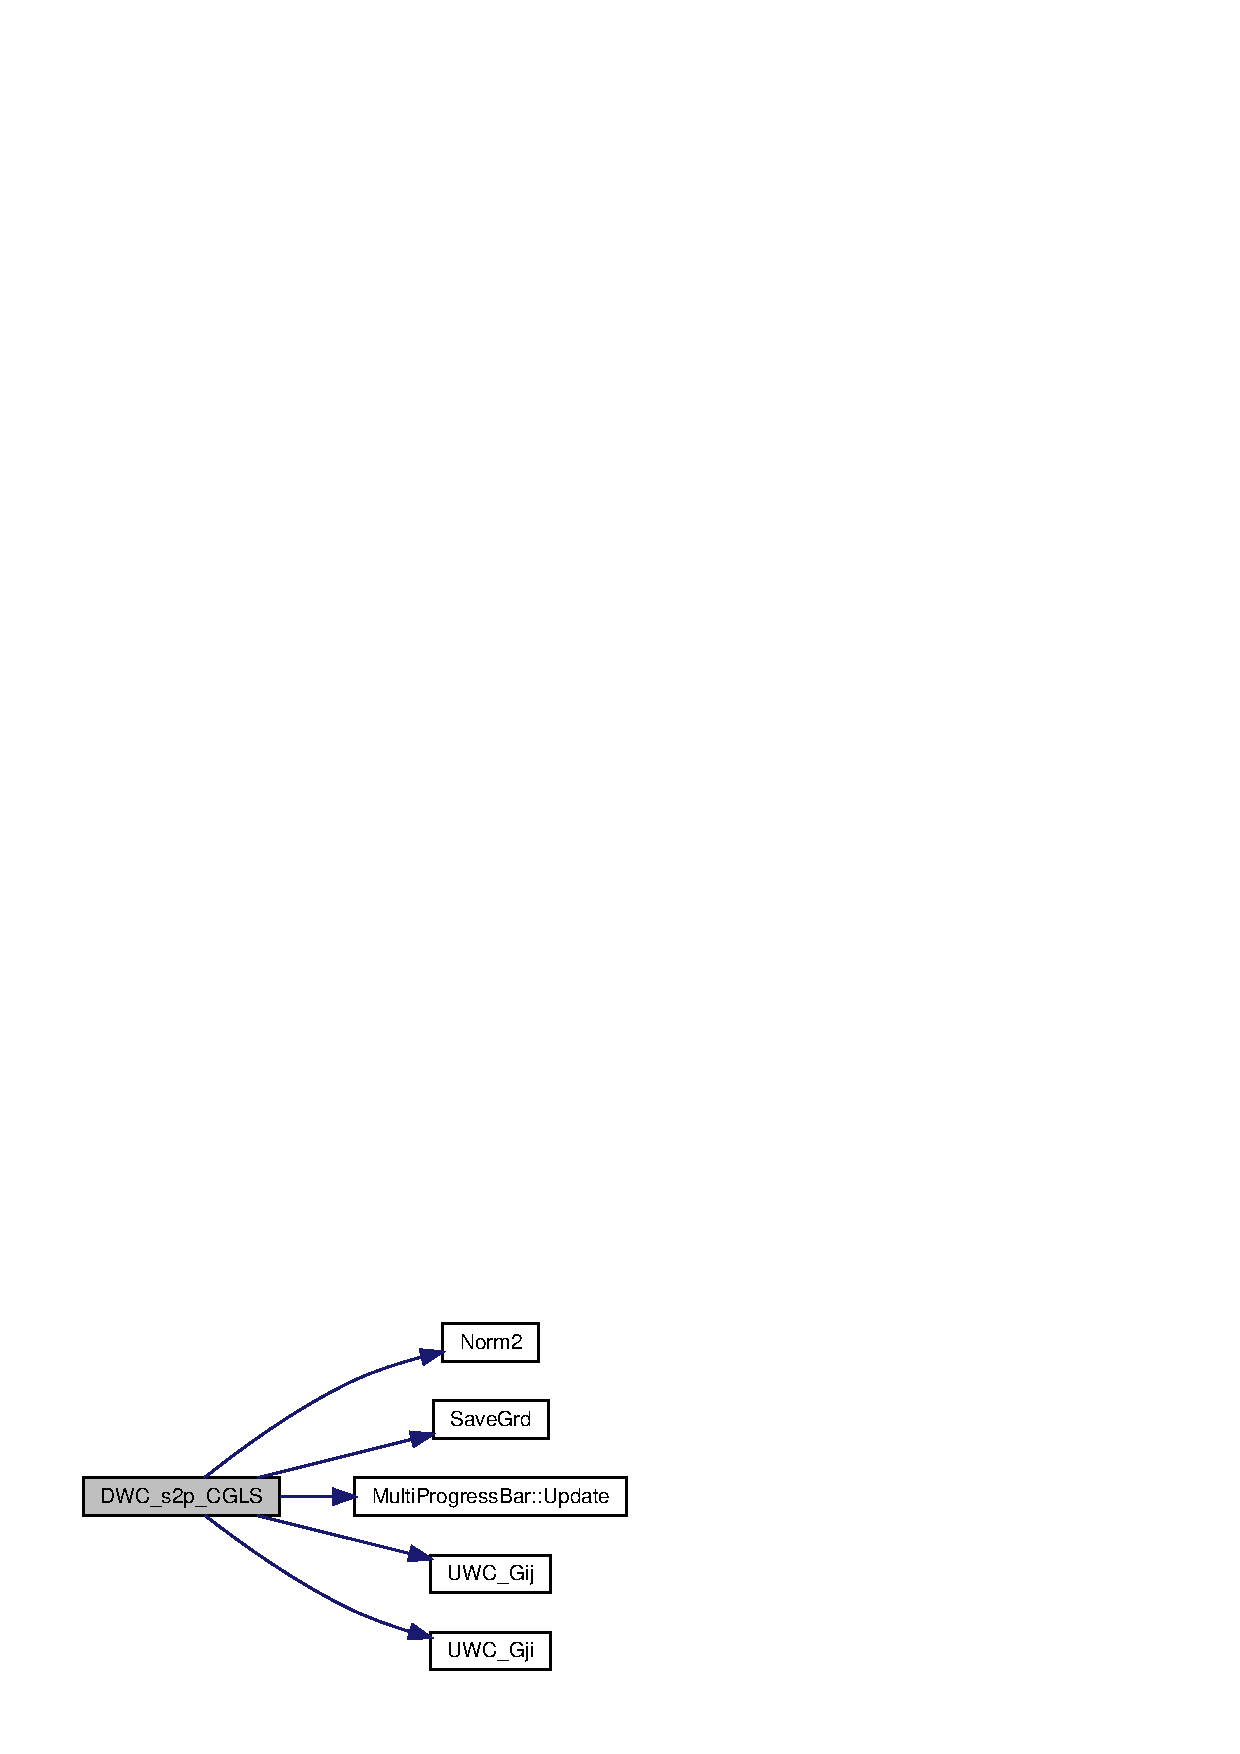
\includegraphics[width=305pt]{Conti2D_8cpp_a6516cfeb71abcf844b32f101e5f77a71_a6516cfeb71abcf844b32f101e5f77a71_cgraph}
\end{center}
\end{figure}
Here is the caller graph for this function\+:\nopagebreak
\begin{figure}[H]
\begin{center}
\leavevmode
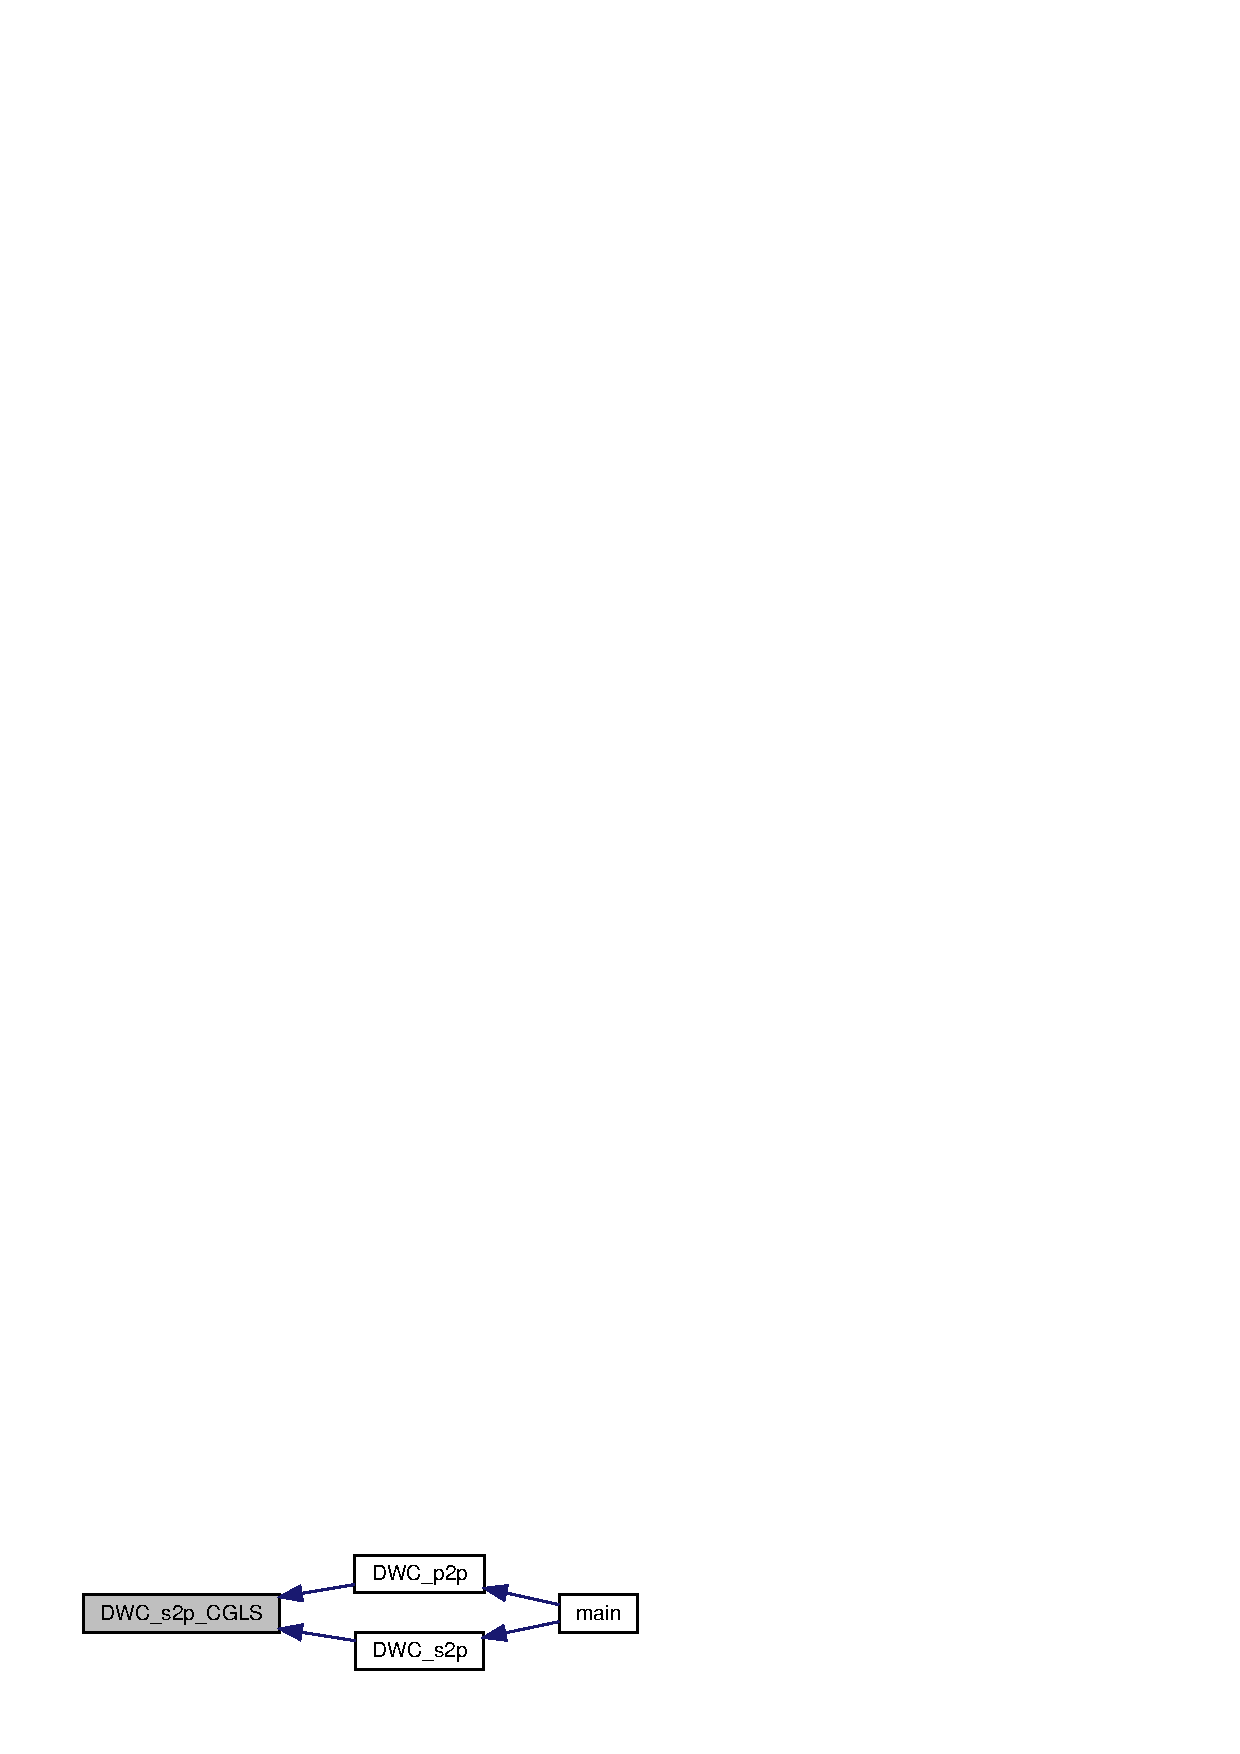
\includegraphics[width=310pt]{Conti2D_8cpp_a6516cfeb71abcf844b32f101e5f77a71_a6516cfeb71abcf844b32f101e5f77a71_icgraph}
\end{center}
\end{figure}
\mbox{\label{Conti2D_8cpp_a0a60bfe4f254fa10e96fabb22a125343_a0a60bfe4f254fa10e96fabb22a125343}} 
\index{Conti2\+D.\+cpp@{Conti2\+D.\+cpp}!D\+W\+C\+\_\+s2p\+\_\+\+Itegration\+Iter@{D\+W\+C\+\_\+s2p\+\_\+\+Itegration\+Iter}}
\index{D\+W\+C\+\_\+s2p\+\_\+\+Itegration\+Iter@{D\+W\+C\+\_\+s2p\+\_\+\+Itegration\+Iter}!Conti2\+D.\+cpp@{Conti2\+D.\+cpp}}
\subsubsection{D\+W\+C\+\_\+s2p\+\_\+\+Itegration\+Iter()}
{\footnotesize\ttfamily void D\+W\+C\+\_\+s2p\+\_\+\+Itegration\+Iter (\begin{DoxyParamCaption}\item[{double $\ast$$\ast$}]{G,  }\item[{double $\ast$}]{x,  }\item[{double $\ast$}]{b,  }\item[{\textbf{ Grd\+Head}}]{grdhead,  }\item[{int}]{ext\+Num,  }\item[{int}]{num\+\_\+thread,  }\item[{string}]{outputfile,  }\item[{double}]{iter\+\_\+number,  }\item[{double $\ast$}]{Exact\+Solution }\end{DoxyParamCaption})}



Definition at line 1317 of file Conti2\+D.\+cpp.



References C\+O\+L\+O\+R\+\_\+\+D\+E\+F\+A\+L\+UT, Grd\+Head\+::cols, G\+R\+E\+EN, Norm2(), Norm2\+\_\+\+Gradient(), Path\+\_\+\+Get\+File\+Name(), R\+ED, Grd\+Head\+::rows, Save\+Grd(), Multi\+Progress\+Bar\+::\+Update(), and U\+W\+C\+\_\+\+Gij().



Referenced by D\+W\+C\+\_\+p2p(), and D\+W\+C\+\_\+s2p().

Here is the call graph for this function\+:
\nopagebreak
\begin{figure}[H]
\begin{center}
\leavevmode
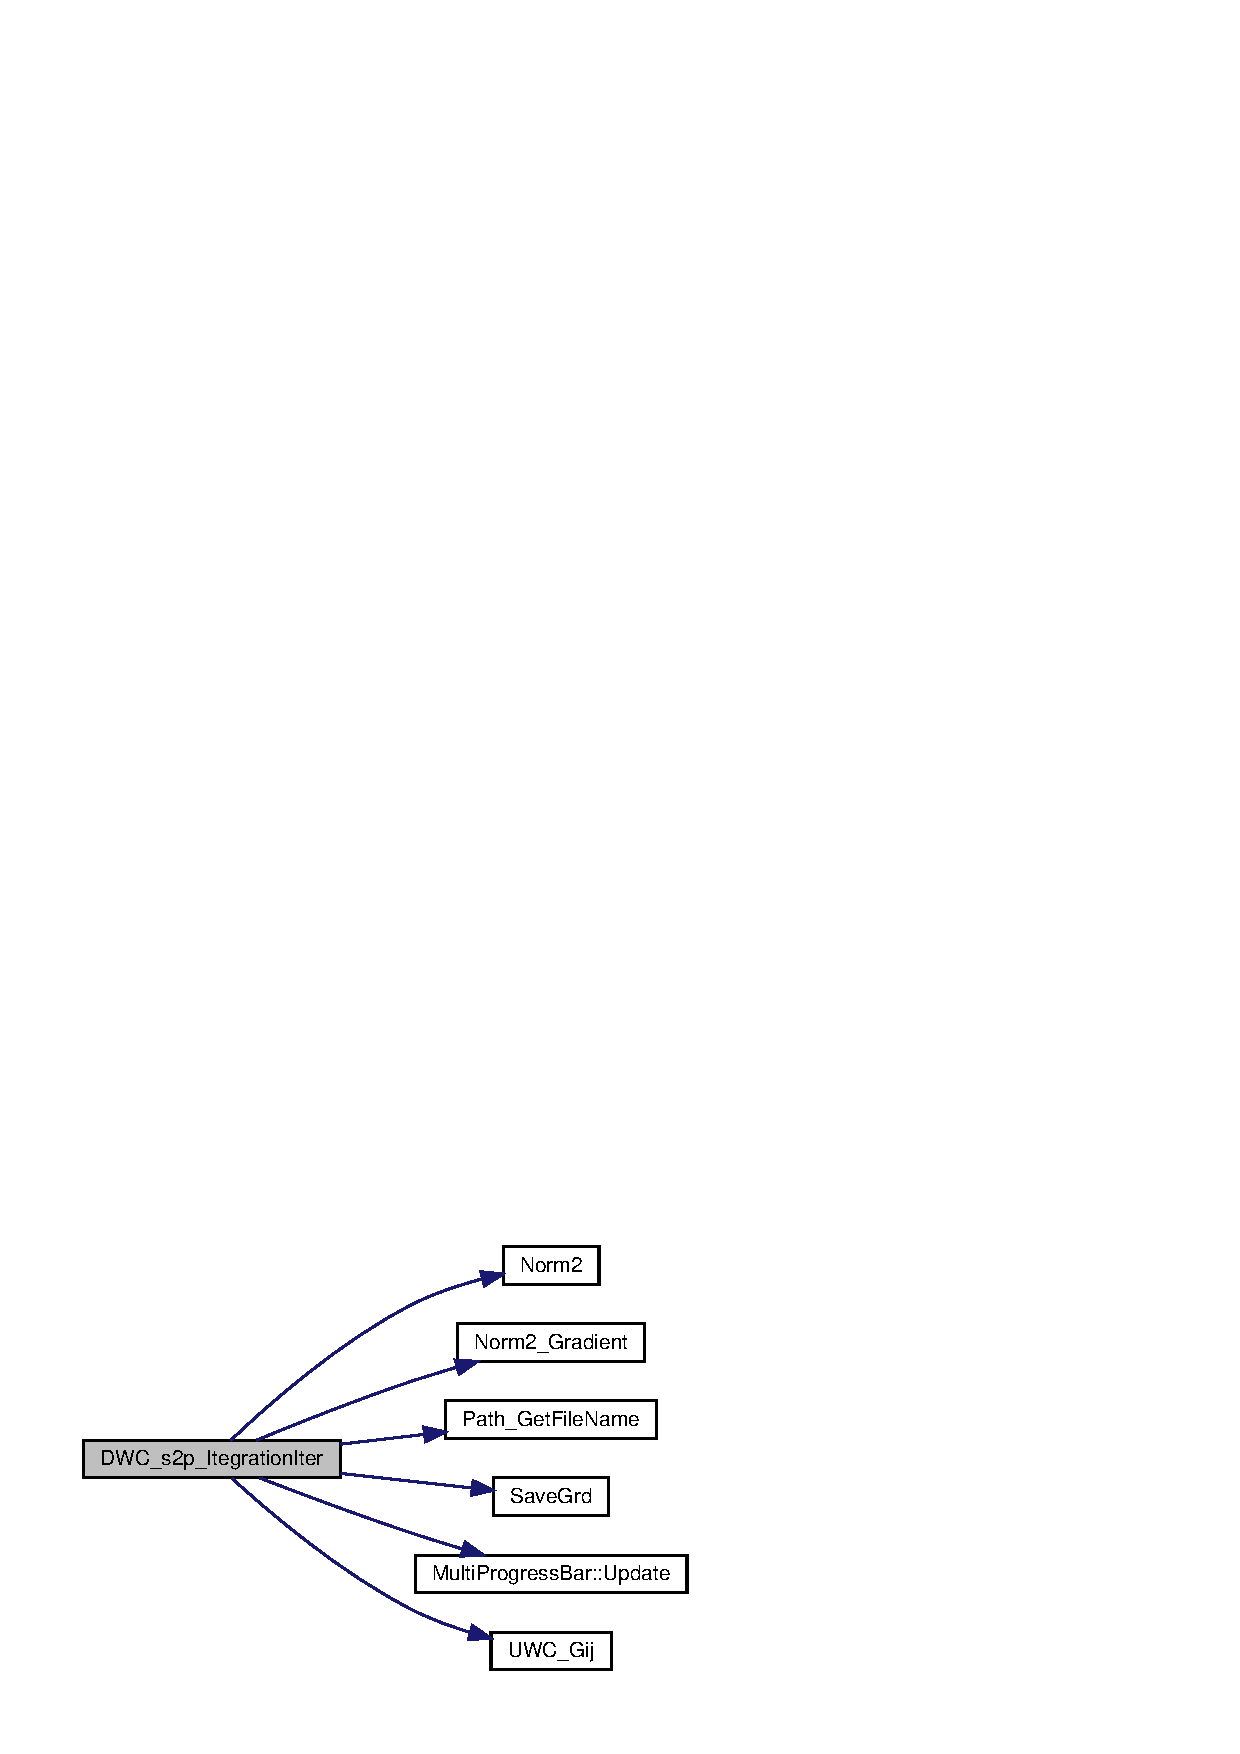
\includegraphics[width=334pt]{Conti2D_8cpp_a0a60bfe4f254fa10e96fabb22a125343_a0a60bfe4f254fa10e96fabb22a125343_cgraph}
\end{center}
\end{figure}
Here is the caller graph for this function\+:\nopagebreak
\begin{figure}[H]
\begin{center}
\leavevmode
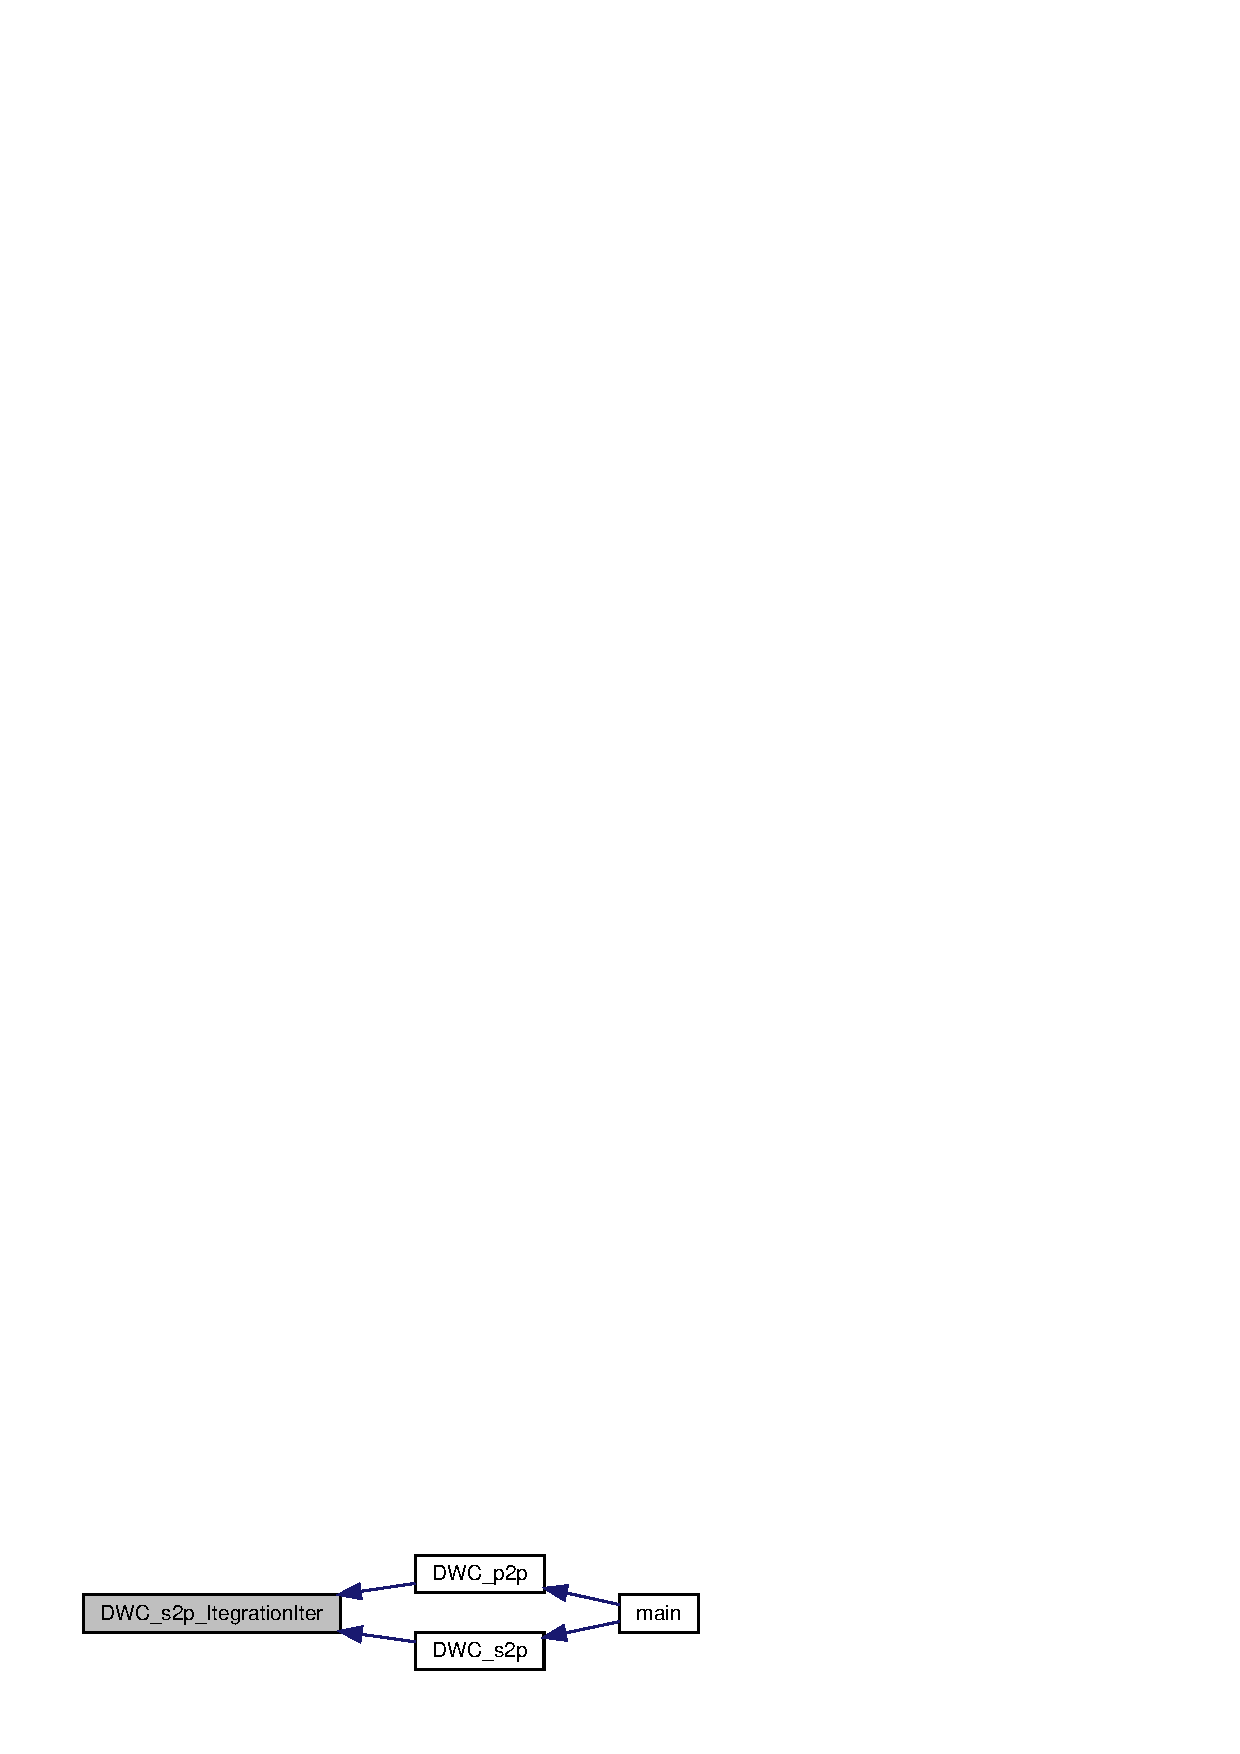
\includegraphics[width=339pt]{Conti2D_8cpp_a0a60bfe4f254fa10e96fabb22a125343_a0a60bfe4f254fa10e96fabb22a125343_icgraph}
\end{center}
\end{figure}
\mbox{\label{Conti2D_8cpp_a7730328c8e132ff0a35142a6d31bac18_a7730328c8e132ff0a35142a6d31bac18}} 
\index{Conti2\+D.\+cpp@{Conti2\+D.\+cpp}!D\+W\+C\+\_\+s2p\+\_\+\+Landweber\+Iter@{D\+W\+C\+\_\+s2p\+\_\+\+Landweber\+Iter}}
\index{D\+W\+C\+\_\+s2p\+\_\+\+Landweber\+Iter@{D\+W\+C\+\_\+s2p\+\_\+\+Landweber\+Iter}!Conti2\+D.\+cpp@{Conti2\+D.\+cpp}}
\subsubsection{D\+W\+C\+\_\+s2p\+\_\+\+Landweber\+Iter()}
{\footnotesize\ttfamily void D\+W\+C\+\_\+s2p\+\_\+\+Landweber\+Iter (\begin{DoxyParamCaption}\item[{double $\ast$$\ast$}]{G,  }\item[{double $\ast$}]{x,  }\item[{double $\ast$}]{b,  }\item[{\textbf{ Grd\+Head}}]{grdhead,  }\item[{int}]{ext\+Num,  }\item[{int}]{num\+\_\+thread,  }\item[{string}]{outputfile,  }\item[{double}]{iter\+\_\+number,  }\item[{double $\ast$}]{Exact\+Solution }\end{DoxyParamCaption})}



Definition at line 1930 of file Conti2\+D.\+cpp.



References C\+O\+L\+O\+R\+\_\+\+D\+E\+F\+A\+L\+UT, Grd\+Head\+::cols, G\+R\+E\+EN, Norm2(), Norm2\+\_\+\+Gradient(), Path\+\_\+\+Get\+File\+Name(), R\+ED, Grd\+Head\+::rows, Save\+Grd(), Multi\+Progress\+Bar\+::\+Update(), and U\+W\+C\+\_\+\+Gij().



Referenced by D\+W\+C\+\_\+p2p(), and D\+W\+C\+\_\+s2p().

Here is the call graph for this function\+:
\nopagebreak
\begin{figure}[H]
\begin{center}
\leavevmode
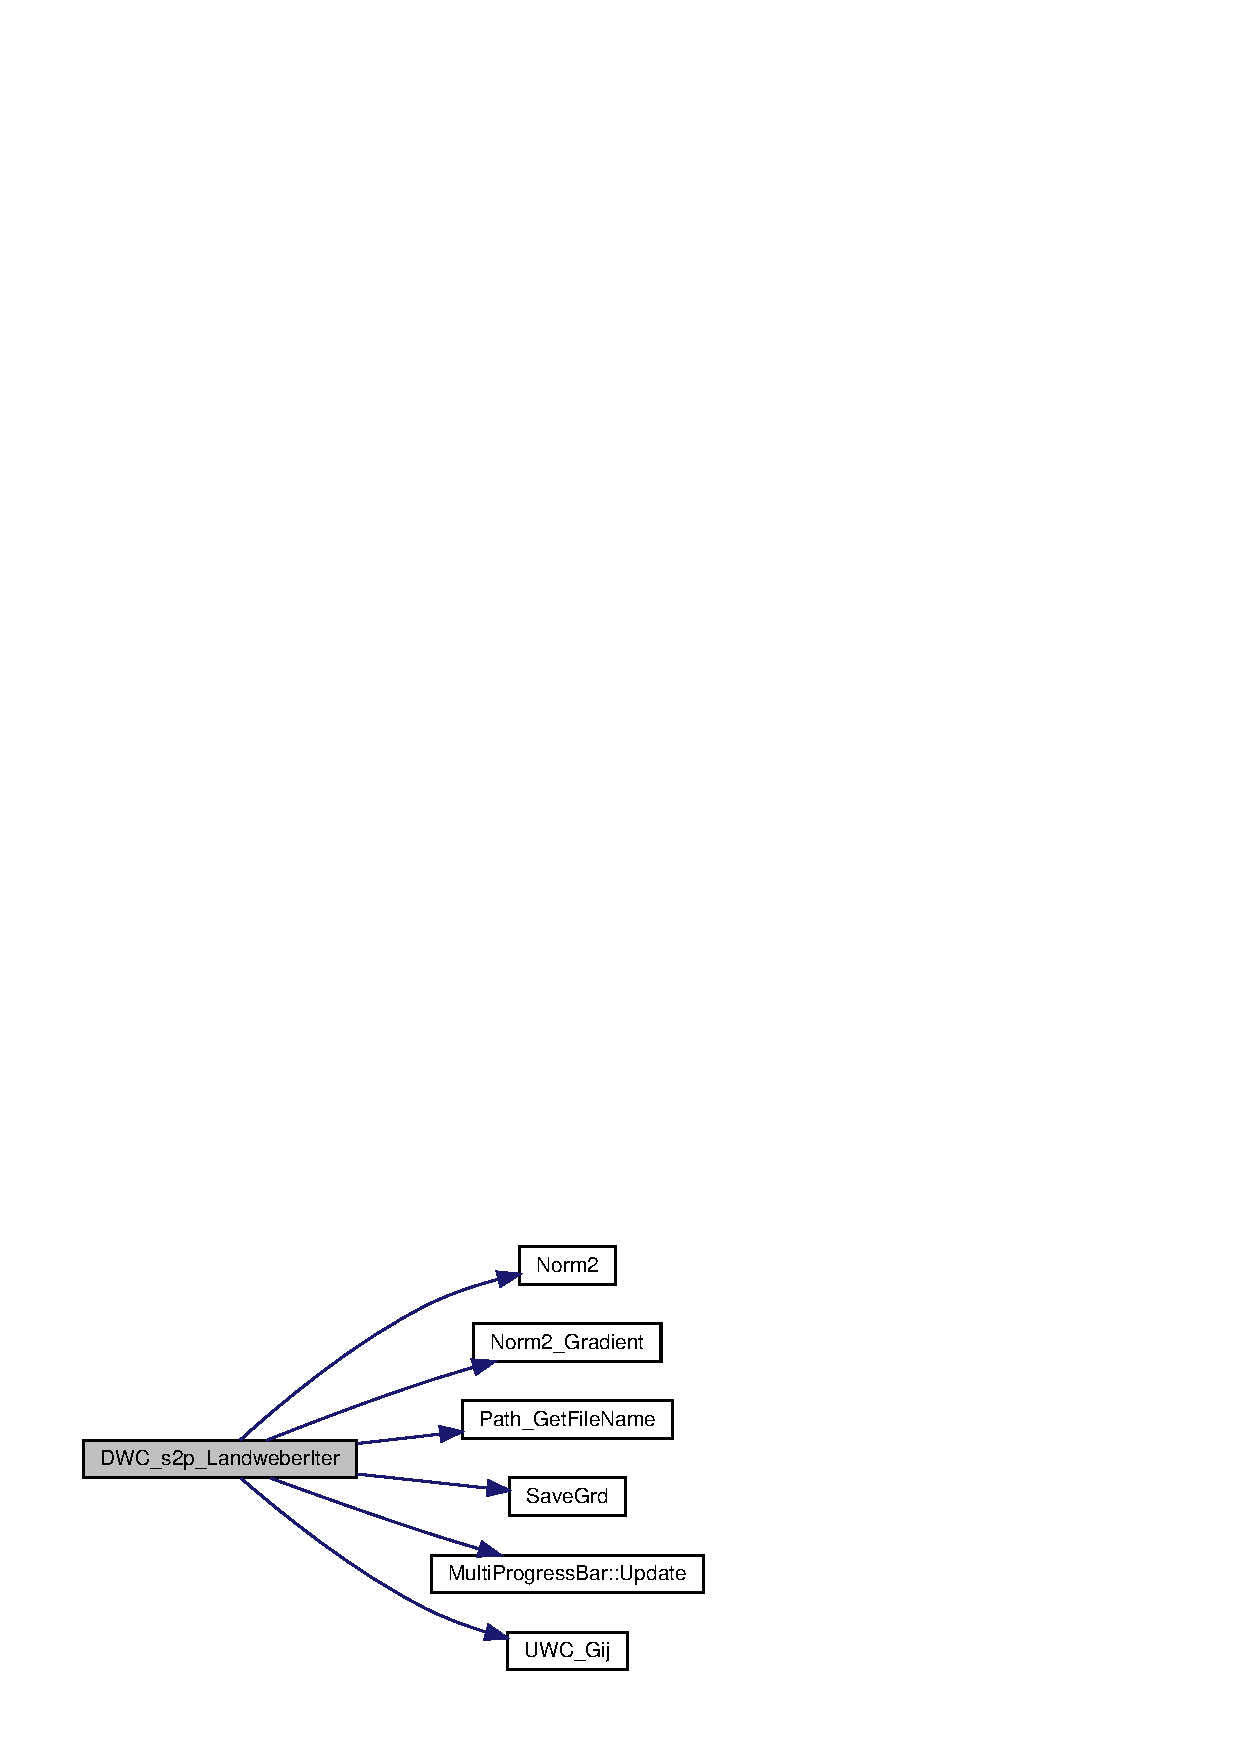
\includegraphics[width=342pt]{Conti2D_8cpp_a7730328c8e132ff0a35142a6d31bac18_a7730328c8e132ff0a35142a6d31bac18_cgraph}
\end{center}
\end{figure}
Here is the caller graph for this function\+:\nopagebreak
\begin{figure}[H]
\begin{center}
\leavevmode
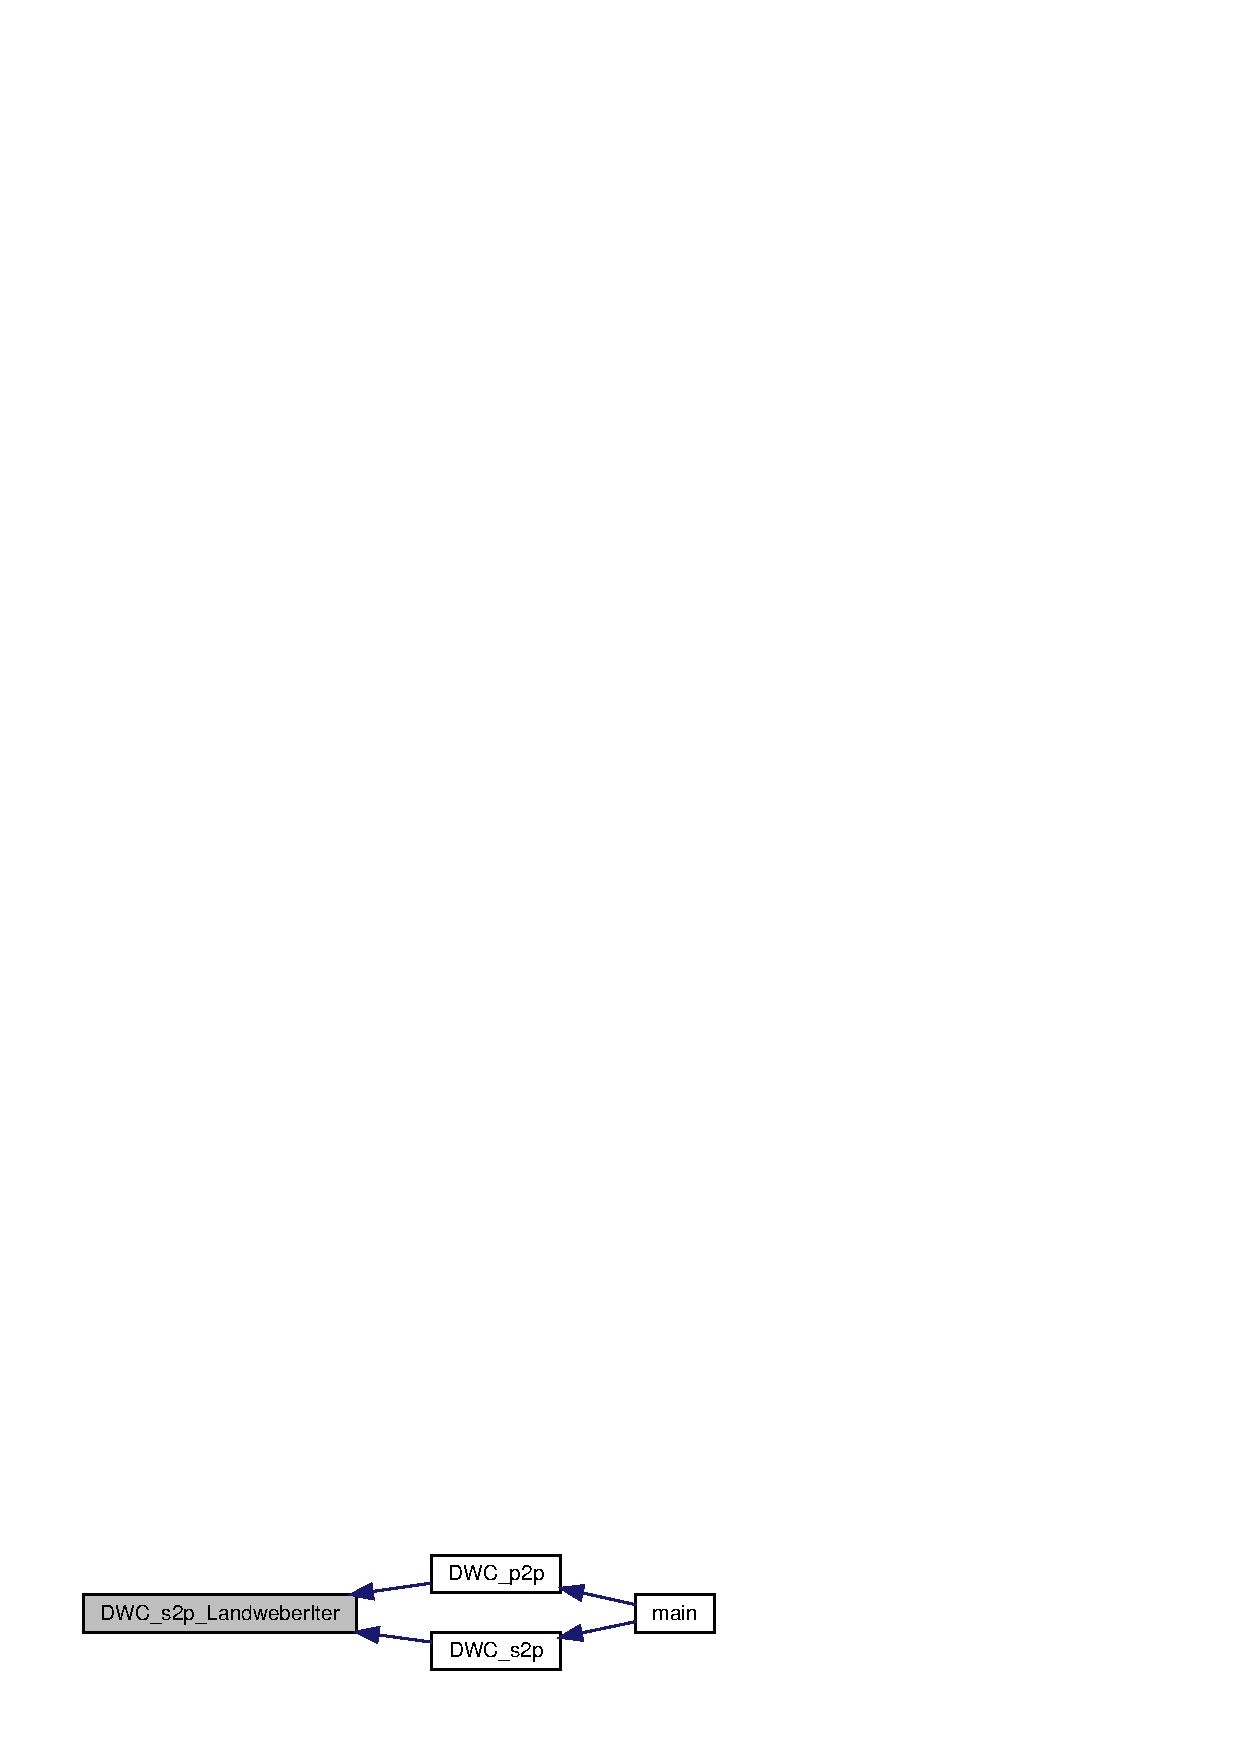
\includegraphics[width=347pt]{Conti2D_8cpp_a7730328c8e132ff0a35142a6d31bac18_a7730328c8e132ff0a35142a6d31bac18_icgraph}
\end{center}
\end{figure}
\mbox{\label{Conti2D_8cpp_abe7855476a24f6e1aa660919f2824d27_abe7855476a24f6e1aa660919f2824d27}} 
\index{Conti2\+D.\+cpp@{Conti2\+D.\+cpp}!D\+W\+C\+\_\+s2p\+\_\+\+Tikhonov@{D\+W\+C\+\_\+s2p\+\_\+\+Tikhonov}}
\index{D\+W\+C\+\_\+s2p\+\_\+\+Tikhonov@{D\+W\+C\+\_\+s2p\+\_\+\+Tikhonov}!Conti2\+D.\+cpp@{Conti2\+D.\+cpp}}
\subsubsection{D\+W\+C\+\_\+s2p\+\_\+\+Tikhonov()}
{\footnotesize\ttfamily void D\+W\+C\+\_\+s2p\+\_\+\+Tikhonov (\begin{DoxyParamCaption}\item[{double $\ast$$\ast$}]{G,  }\item[{double $\ast$}]{x,  }\item[{double $\ast$}]{b0,  }\item[{\textbf{ Grd\+Head}}]{grdhead,  }\item[{int}]{ext\+Num,  }\item[{double}]{lambda,  }\item[{int}]{num\+\_\+thread }\end{DoxyParamCaption})}



Definition at line 1580 of file Conti2\+D.\+cpp.



References Grd\+Head\+::cols, Norm2(), Grd\+Head\+::rows, Save\+Grd(), Multi\+Progress\+Bar\+::\+Update(), U\+W\+C\+\_\+\+G\+\_\+\+C\+G\+L\+S\+\_\+\+Tik(), and U\+W\+C\+\_\+\+Gji().

Here is the call graph for this function\+:
\nopagebreak
\begin{figure}[H]
\begin{center}
\leavevmode
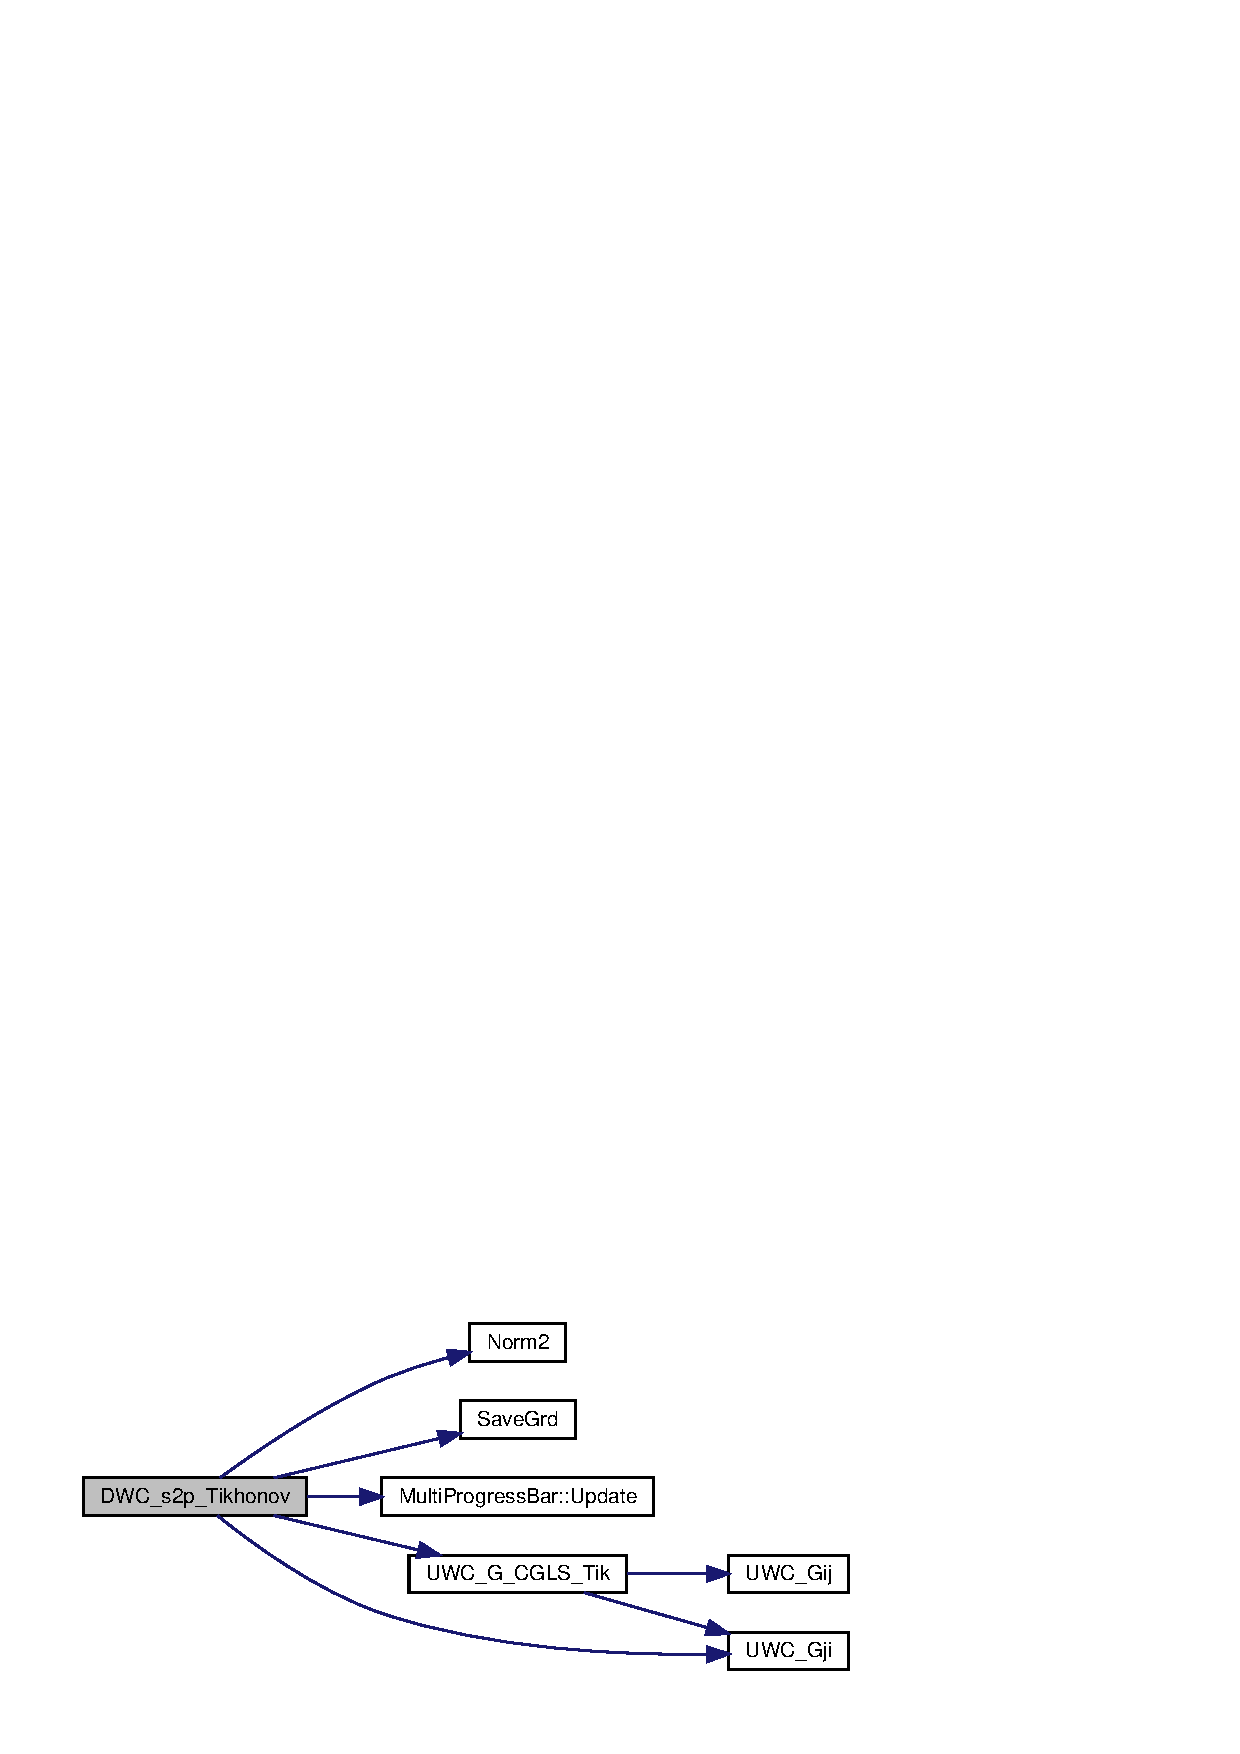
\includegraphics[width=350pt]{Conti2D_8cpp_abe7855476a24f6e1aa660919f2824d27_abe7855476a24f6e1aa660919f2824d27_cgraph}
\end{center}
\end{figure}
\mbox{\label{Conti2D_8cpp_aca8df189bd3e80e2041b22f7691d87b0_aca8df189bd3e80e2041b22f7691d87b0}} 
\index{Conti2\+D.\+cpp@{Conti2\+D.\+cpp}!D\+W\+C\+\_\+\+Tikhonov\+\_\+old@{D\+W\+C\+\_\+\+Tikhonov\+\_\+old}}
\index{D\+W\+C\+\_\+\+Tikhonov\+\_\+old@{D\+W\+C\+\_\+\+Tikhonov\+\_\+old}!Conti2\+D.\+cpp@{Conti2\+D.\+cpp}}
\subsubsection{D\+W\+C\+\_\+\+Tikhonov\+\_\+old()}
{\footnotesize\ttfamily void D\+W\+C\+\_\+\+Tikhonov\+\_\+old (\begin{DoxyParamCaption}\item[{double $\ast$}]{G\+\_\+first\+Row,  }\item[{double $\ast$}]{dataout,  }\item[{double $\ast$}]{indata,  }\item[{double}]{T\+RP,  }\item[{int}]{kmax,  }\item[{double}]{daierta,  }\item[{\textbf{ Grd\+Head}}]{grdhead,  }\item[{int}]{num\+\_\+thread }\end{DoxyParamCaption})}



Definition at line 2016 of file Conti2\+D.\+cpp.



References Grd\+Head\+::cols, Grd\+Head\+::rows, and U\+W\+C\+\_\+\+Gij().

Here is the call graph for this function\+:\nopagebreak
\begin{figure}[H]
\begin{center}
\leavevmode
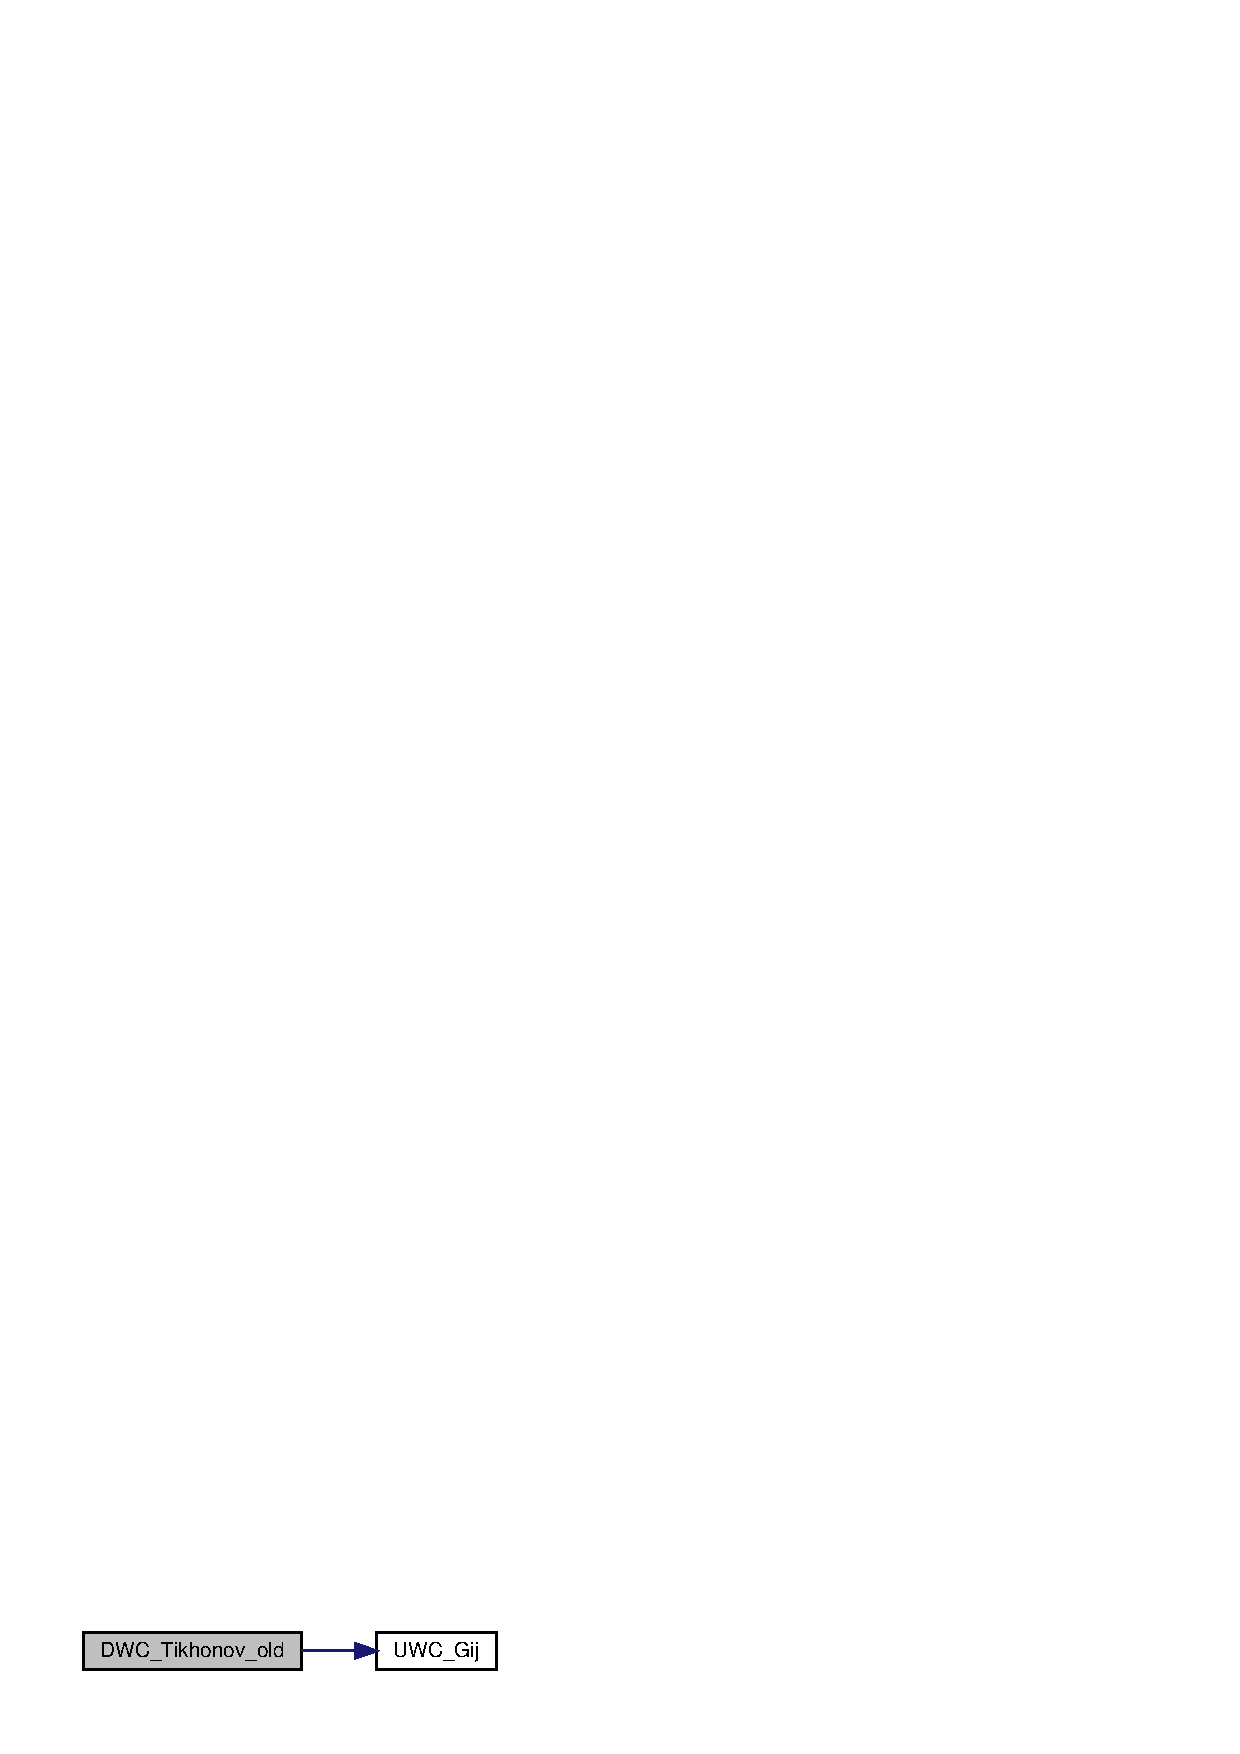
\includegraphics[width=242pt]{Conti2D_8cpp_aca8df189bd3e80e2041b22f7691d87b0_aca8df189bd3e80e2041b22f7691d87b0_cgraph}
\end{center}
\end{figure}
\mbox{\label{Conti2D_8cpp_abb92297fdfe4c3fea02efc2311fb9019_abb92297fdfe4c3fea02efc2311fb9019}} 
\index{Conti2\+D.\+cpp@{Conti2\+D.\+cpp}!Get\+Gij@{Get\+Gij}}
\index{Get\+Gij@{Get\+Gij}!Conti2\+D.\+cpp@{Conti2\+D.\+cpp}}
\subsubsection{Get\+Gij()}
{\footnotesize\ttfamily double Get\+Gij (\begin{DoxyParamCaption}\item[{const int}]{i,  }\item[{const int}]{j,  }\item[{double $\ast$}]{first\+Row,  }\item[{const \textbf{ Grd\+Head}}]{grdhead }\end{DoxyParamCaption})}



Get the value at i row and the j column of kernel matrix from the first row of the matrix only. 


\begin{DoxyParams}{Parameters}
{\em i} & \\
\hline
{\em j} & \\
\hline
{\em first\+Row} & The first row of the kernel matrix \\
\hline
{\em grdhead} & \\
\hline
\end{DoxyParams}
\begin{DoxyReturn}{Returns}
double 
\end{DoxyReturn}


Definition at line 138 of file Conti2\+D.\+cpp.



References Grd\+Head\+::cols, and Grd\+Head\+::rows.



Referenced by U\+W\+C\+\_\+\+Gij(), and U\+W\+C\+\_\+\+Gji().

Here is the caller graph for this function\+:\nopagebreak
\begin{figure}[H]
\begin{center}
\leavevmode
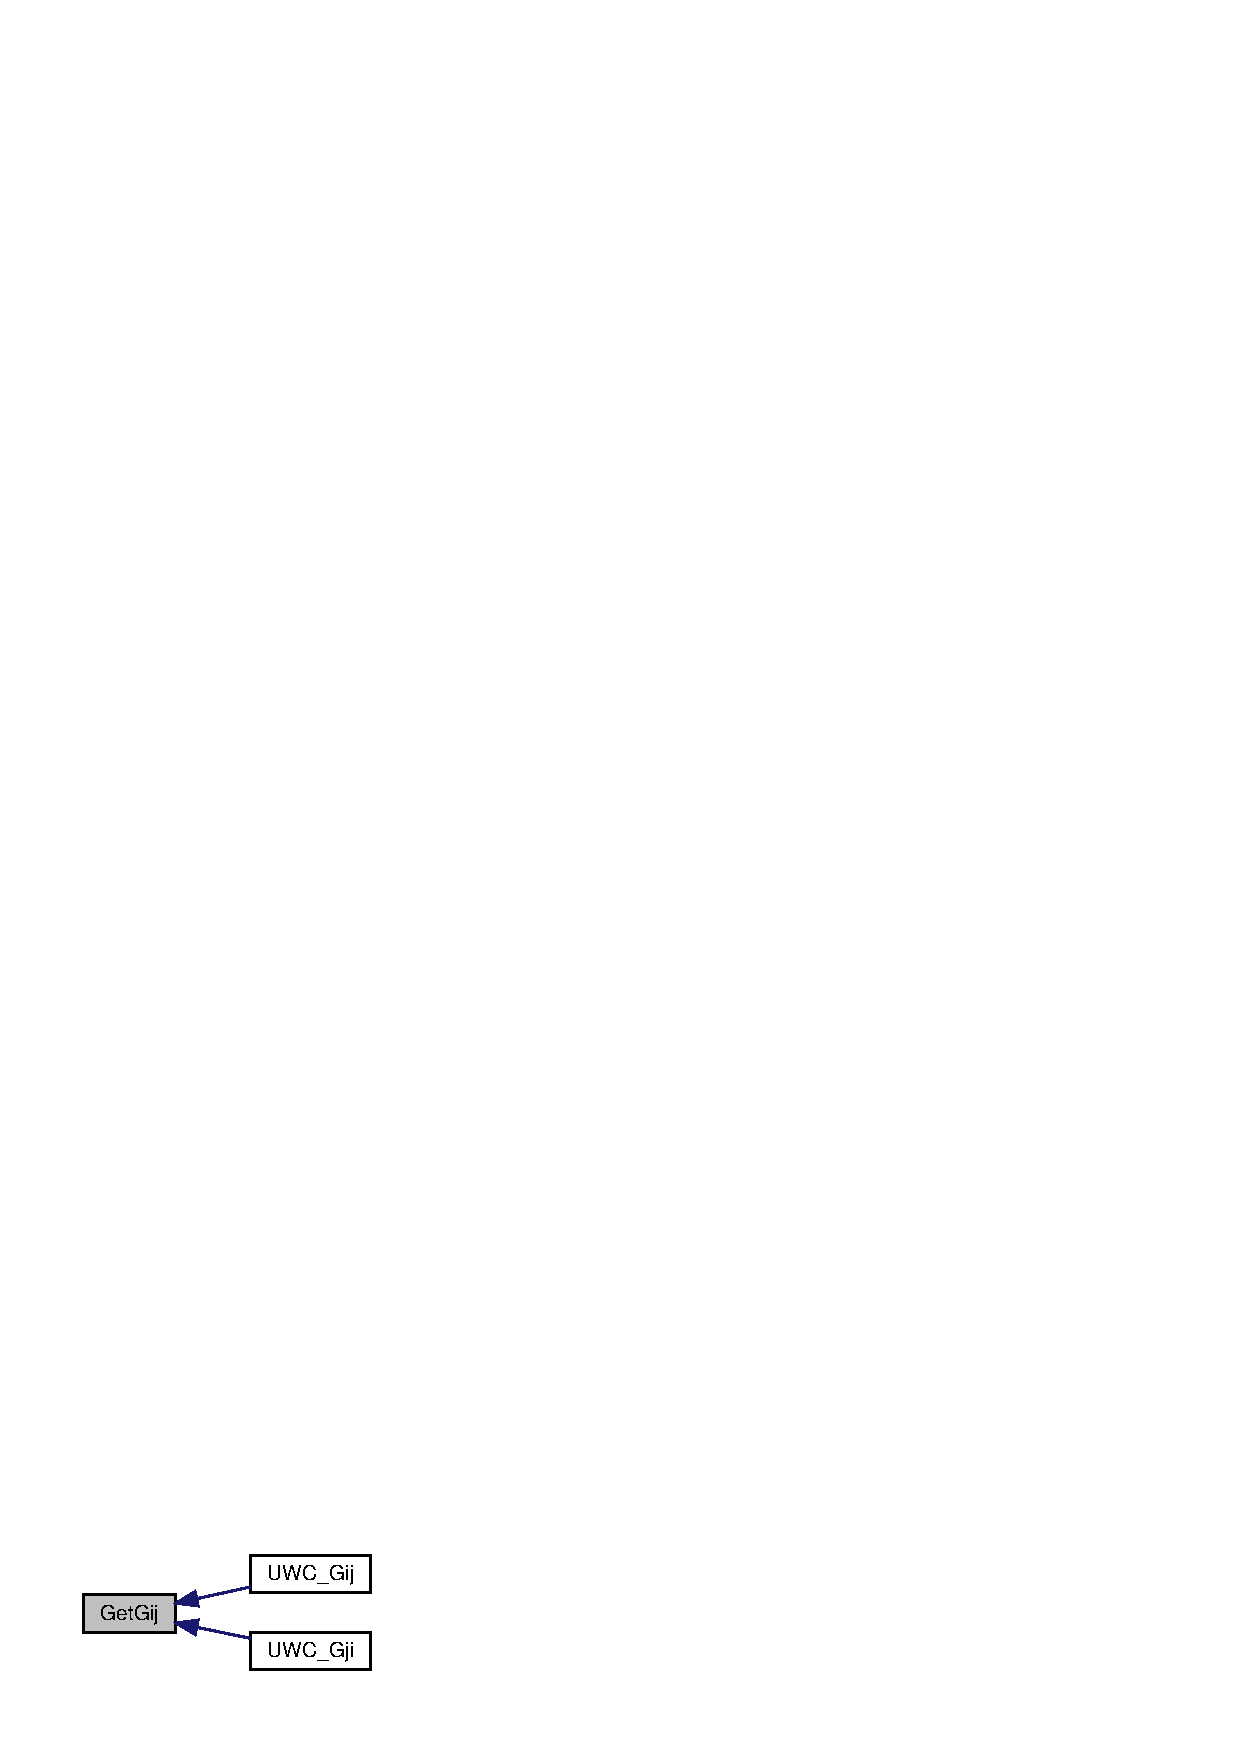
\includegraphics[width=182pt]{Conti2D_8cpp_abb92297fdfe4c3fea02efc2311fb9019_abb92297fdfe4c3fea02efc2311fb9019_icgraph}
\end{center}
\end{figure}
\mbox{\label{Conti2D_8cpp_ac2a0a3da98913cf6500803df23752fd6_ac2a0a3da98913cf6500803df23752fd6}} 
\index{Conti2\+D.\+cpp@{Conti2\+D.\+cpp}!Get\+Kernal\+Matrix@{Get\+Kernal\+Matrix}}
\index{Get\+Kernal\+Matrix@{Get\+Kernal\+Matrix}!Conti2\+D.\+cpp@{Conti2\+D.\+cpp}}
\subsubsection{Get\+Kernal\+Matrix()}
{\footnotesize\ttfamily void Get\+Kernal\+Matrix (\begin{DoxyParamCaption}\item[{\textbf{ Grd\+Head}}]{grdhead,  }\item[{double $\ast$}]{G,  }\item[{const double}]{rph,  }\item[{int}]{num\+\_\+thread = {\ttfamily 4} }\end{DoxyParamCaption})}



Get the Kernal Matrix object. 


\begin{DoxyParams}{Parameters}
{\em grdhead} & \\
\hline
{\em G} & \\
\hline
{\em rph} & \\
\hline
{\em num\+\_\+thread} & \\
\hline
\end{DoxyParams}


Definition at line 34 of file Conti2\+D.\+cpp.



References Grd\+Head\+::bounds, Grd\+Head\+::cols, PI, and Grd\+Head\+::rows.

\mbox{\label{Conti2D_8cpp_a8d8d41669d98b597c959db5762cbb489_a8d8d41669d98b597c959db5762cbb489}} 
\index{Conti2\+D.\+cpp@{Conti2\+D.\+cpp}!Get\+Kernal\+Matrix\+\_\+new@{Get\+Kernal\+Matrix\+\_\+new}}
\index{Get\+Kernal\+Matrix\+\_\+new@{Get\+Kernal\+Matrix\+\_\+new}!Conti2\+D.\+cpp@{Conti2\+D.\+cpp}}
\subsubsection{Get\+Kernal\+Matrix\+\_\+new()}
{\footnotesize\ttfamily void Get\+Kernal\+Matrix\+\_\+new (\begin{DoxyParamCaption}\item[{\textbf{ Grd\+Head}}]{grdhead,  }\item[{double $\ast$}]{G,  }\item[{const double}]{rph,  }\item[{int}]{num\+\_\+thread = {\ttfamily 4} }\end{DoxyParamCaption})}



Get the kernel matrix using the new developed formula. 


\begin{DoxyParams}{Parameters}
{\em grdhead} & \\
\hline
{\em G} & a 1-\/d array to store the kernel matrix \\
\hline
{\em rph} & height of continuation \\
\hline
{\em num\+\_\+thread} & \\
\hline
\end{DoxyParams}


Definition at line 75 of file Conti2\+D.\+cpp.



References Grd\+Head\+::bounds, Grd\+Head\+::cols, PI, and Grd\+Head\+::rows.



Referenced by D\+W\+C\+\_\+p2p\+\_\+f().

Here is the caller graph for this function\+:\nopagebreak
\begin{figure}[H]
\begin{center}
\leavevmode
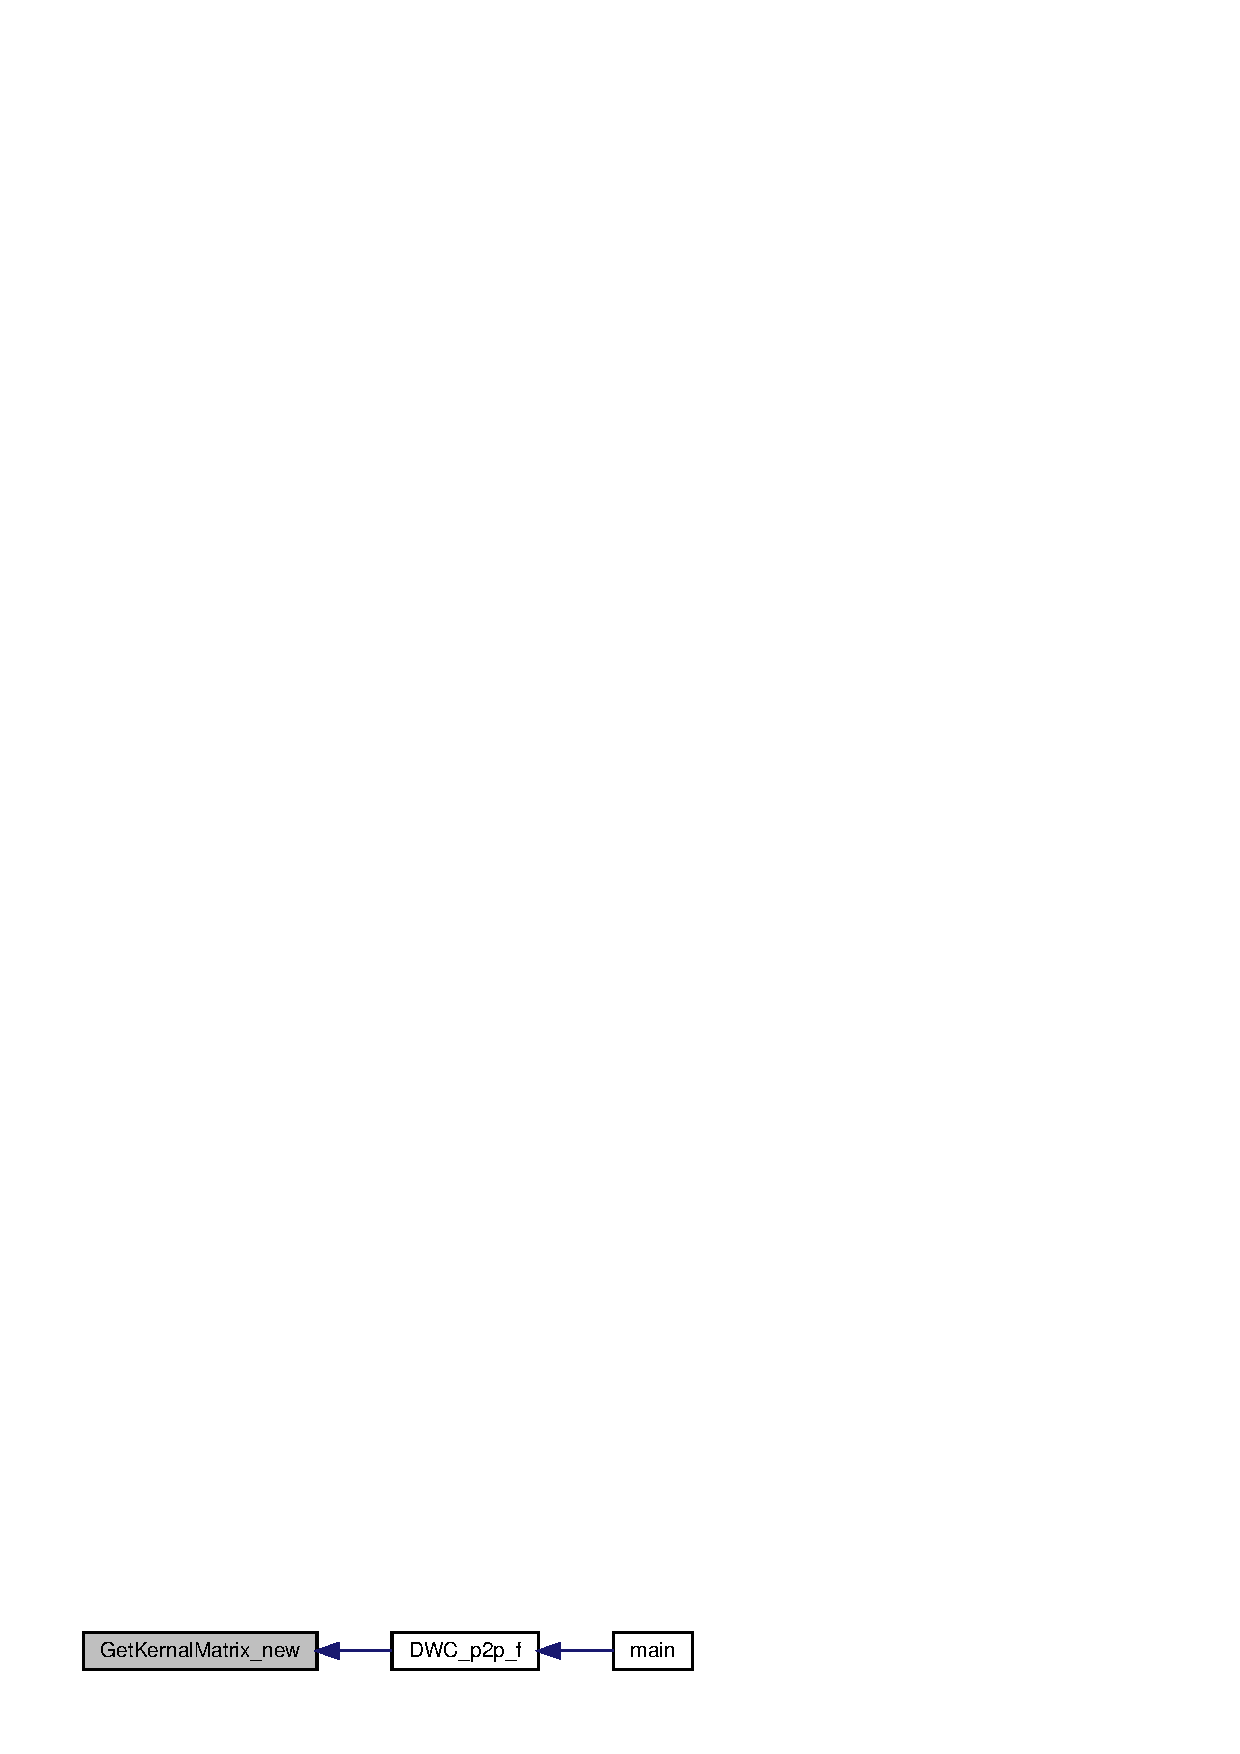
\includegraphics[width=336pt]{Conti2D_8cpp_a8d8d41669d98b597c959db5762cbb489_a8d8d41669d98b597c959db5762cbb489_icgraph}
\end{center}
\end{figure}
\mbox{\label{Conti2D_8cpp_a771b48a44ec12bf118f2fbf3789a7d70_a771b48a44ec12bf118f2fbf3789a7d70}} 
\index{Conti2\+D.\+cpp@{Conti2\+D.\+cpp}!Getkernel\+\_\+p2p@{Getkernel\+\_\+p2p}}
\index{Getkernel\+\_\+p2p@{Getkernel\+\_\+p2p}!Conti2\+D.\+cpp@{Conti2\+D.\+cpp}}
\subsubsection{Getkernel\+\_\+p2p()}
{\footnotesize\ttfamily int Getkernel\+\_\+p2p (\begin{DoxyParamCaption}\item[{\textbf{ Grd\+Head}}]{grdhead,  }\item[{double}]{rph,  }\item[{double $\ast$$\ast$}]{kernel,  }\item[{int}]{num\+\_\+thread }\end{DoxyParamCaption})}



Upward continue from plane to plane. 


\begin{DoxyParams}{Parameters}
{\em grdhead} & \\
\hline
{\em rph} & \\
\hline
{\em kernel} & \\
\hline
{\em num\+\_\+thread} & \\
\hline
\end{DoxyParams}
\begin{DoxyReturn}{Returns}
int 
\end{DoxyReturn}


Definition at line 197 of file Conti2\+D.\+cpp.



References Grd\+Head\+::bounds, Grd\+Head\+::cols, PI, Grd\+Head\+::rows, and Multi\+Progress\+Bar\+::\+Update().

Here is the call graph for this function\+:\nopagebreak
\begin{figure}[H]
\begin{center}
\leavevmode
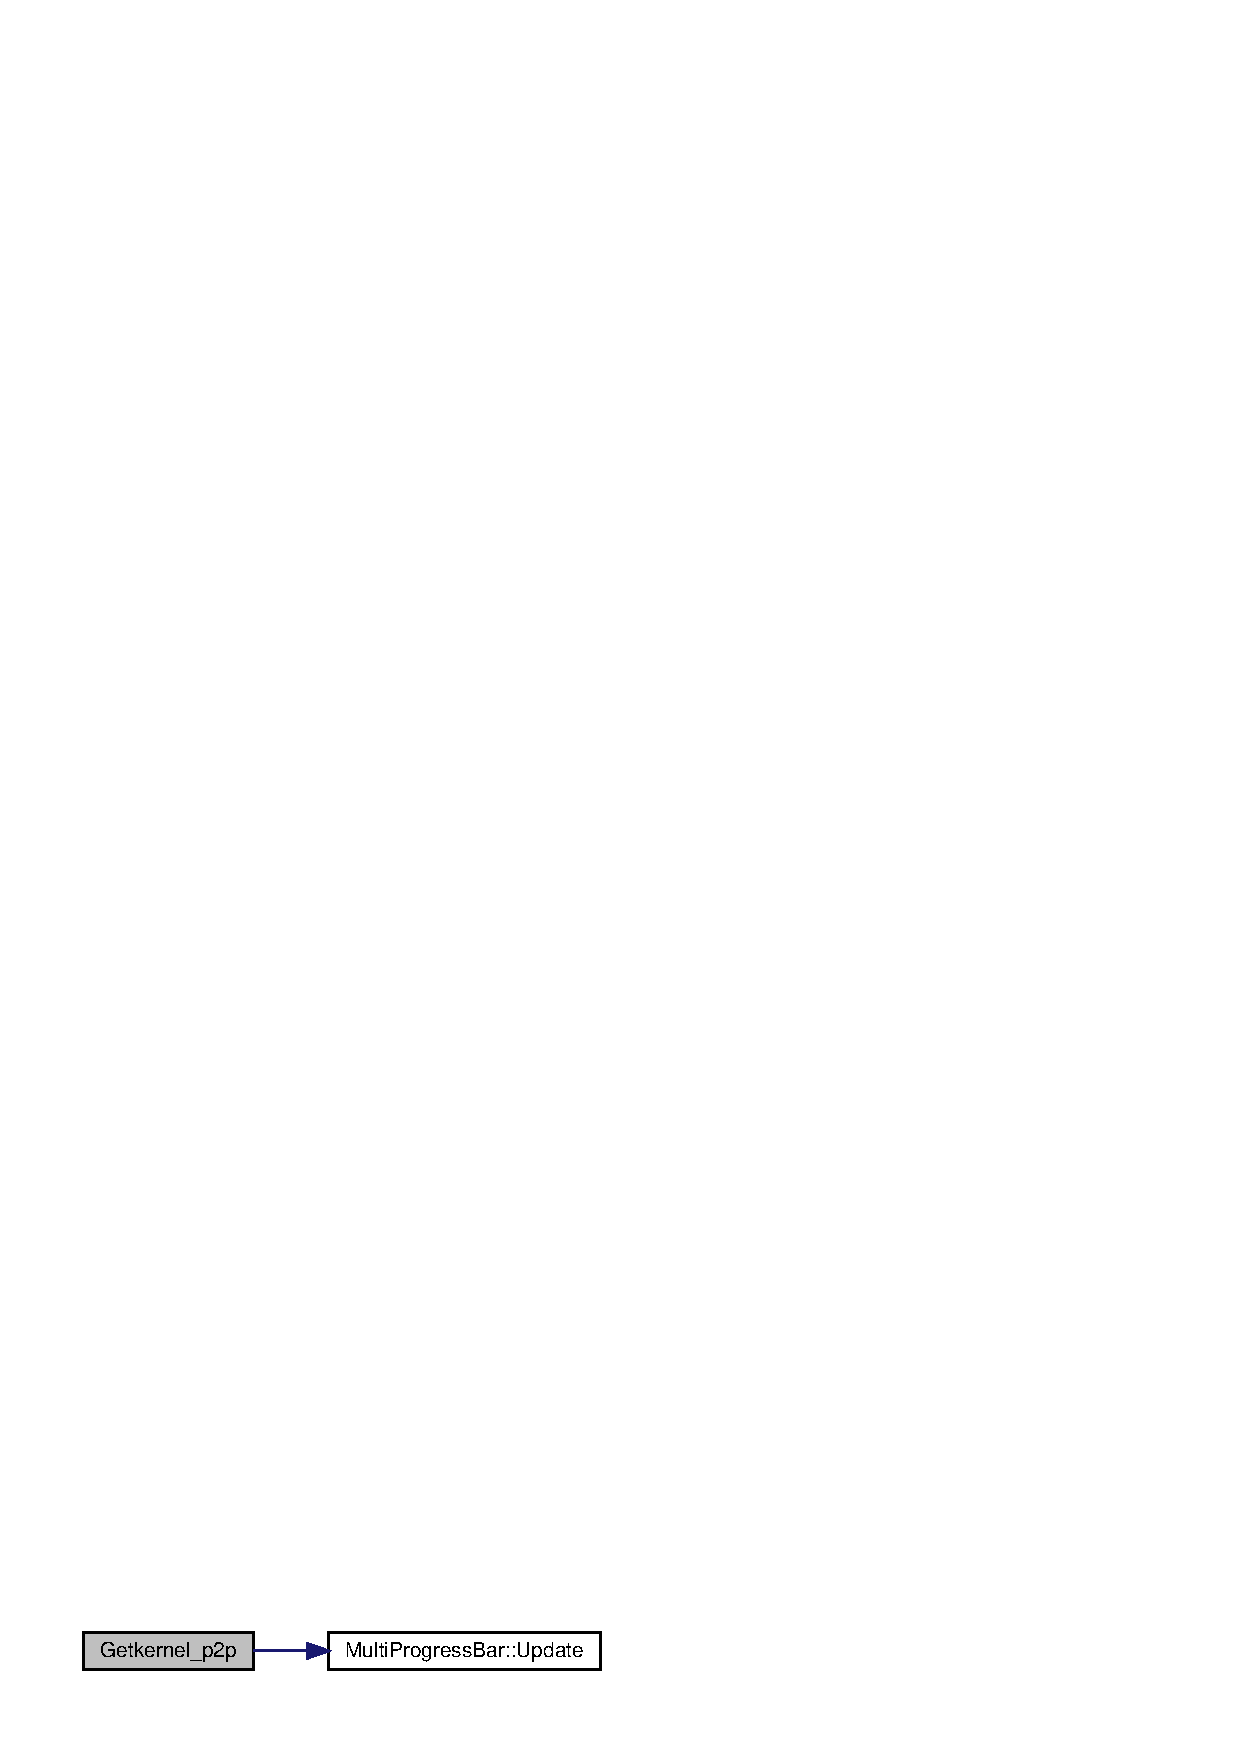
\includegraphics[width=292pt]{Conti2D_8cpp_a771b48a44ec12bf118f2fbf3789a7d70_a771b48a44ec12bf118f2fbf3789a7d70_cgraph}
\end{center}
\end{figure}
\mbox{\label{Conti2D_8cpp_a6f44a06f2b4926f66481fccf277bea50_a6f44a06f2b4926f66481fccf277bea50}} 
\index{Conti2\+D.\+cpp@{Conti2\+D.\+cpp}!Getkernel\+\_\+p2p\+\_\+new@{Getkernel\+\_\+p2p\+\_\+new}}
\index{Getkernel\+\_\+p2p\+\_\+new@{Getkernel\+\_\+p2p\+\_\+new}!Conti2\+D.\+cpp@{Conti2\+D.\+cpp}}
\subsubsection{Getkernel\+\_\+p2p\+\_\+new()\hspace{0.1cm}{\footnotesize\ttfamily [1/2]}}
{\footnotesize\ttfamily int Getkernel\+\_\+p2p\+\_\+new (\begin{DoxyParamCaption}\item[{\textbf{ Grd\+Head}}]{grdhead,  }\item[{double}]{rph,  }\item[{double $\ast$$\ast$}]{kernel,  }\item[{int}]{num\+\_\+thread }\end{DoxyParamCaption})}



Definition at line 271 of file Conti2\+D.\+cpp.



References Grd\+Head\+::bounds, C\+O\+L\+O\+R\+\_\+\+B\+A\+R\+\_\+\+B\+L\+UE, Grd\+Head\+::cols, Get\+Pmnij(), Grd\+Head\+::rows, and Multi\+Progress\+Bar\+::\+Update().



Referenced by D\+W\+C\+\_\+p2p(), and U\+W\+C\+\_\+p2p().

Here is the call graph for this function\+:\nopagebreak
\begin{figure}[H]
\begin{center}
\leavevmode
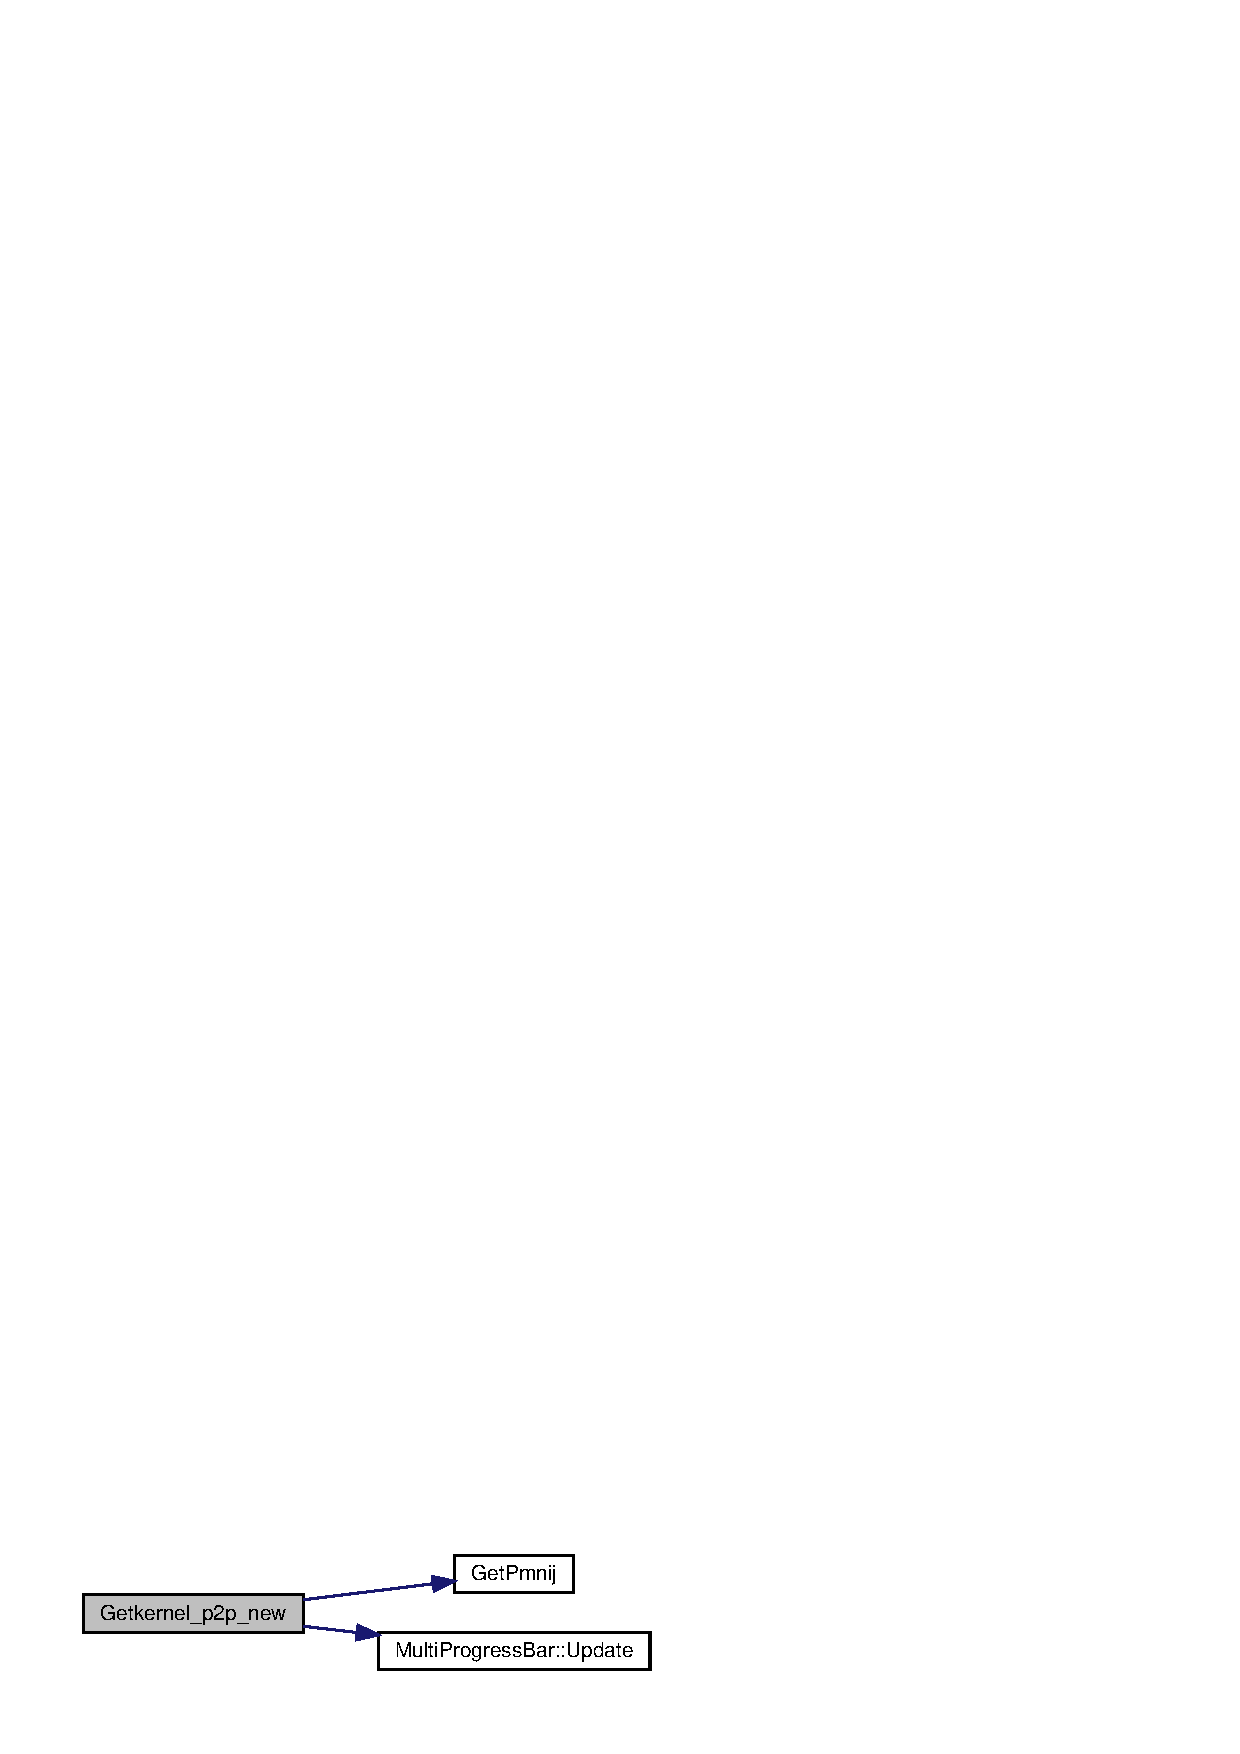
\includegraphics[width=316pt]{Conti2D_8cpp_a6f44a06f2b4926f66481fccf277bea50_a6f44a06f2b4926f66481fccf277bea50_cgraph}
\end{center}
\end{figure}
Here is the caller graph for this function\+:\nopagebreak
\begin{figure}[H]
\begin{center}
\leavevmode
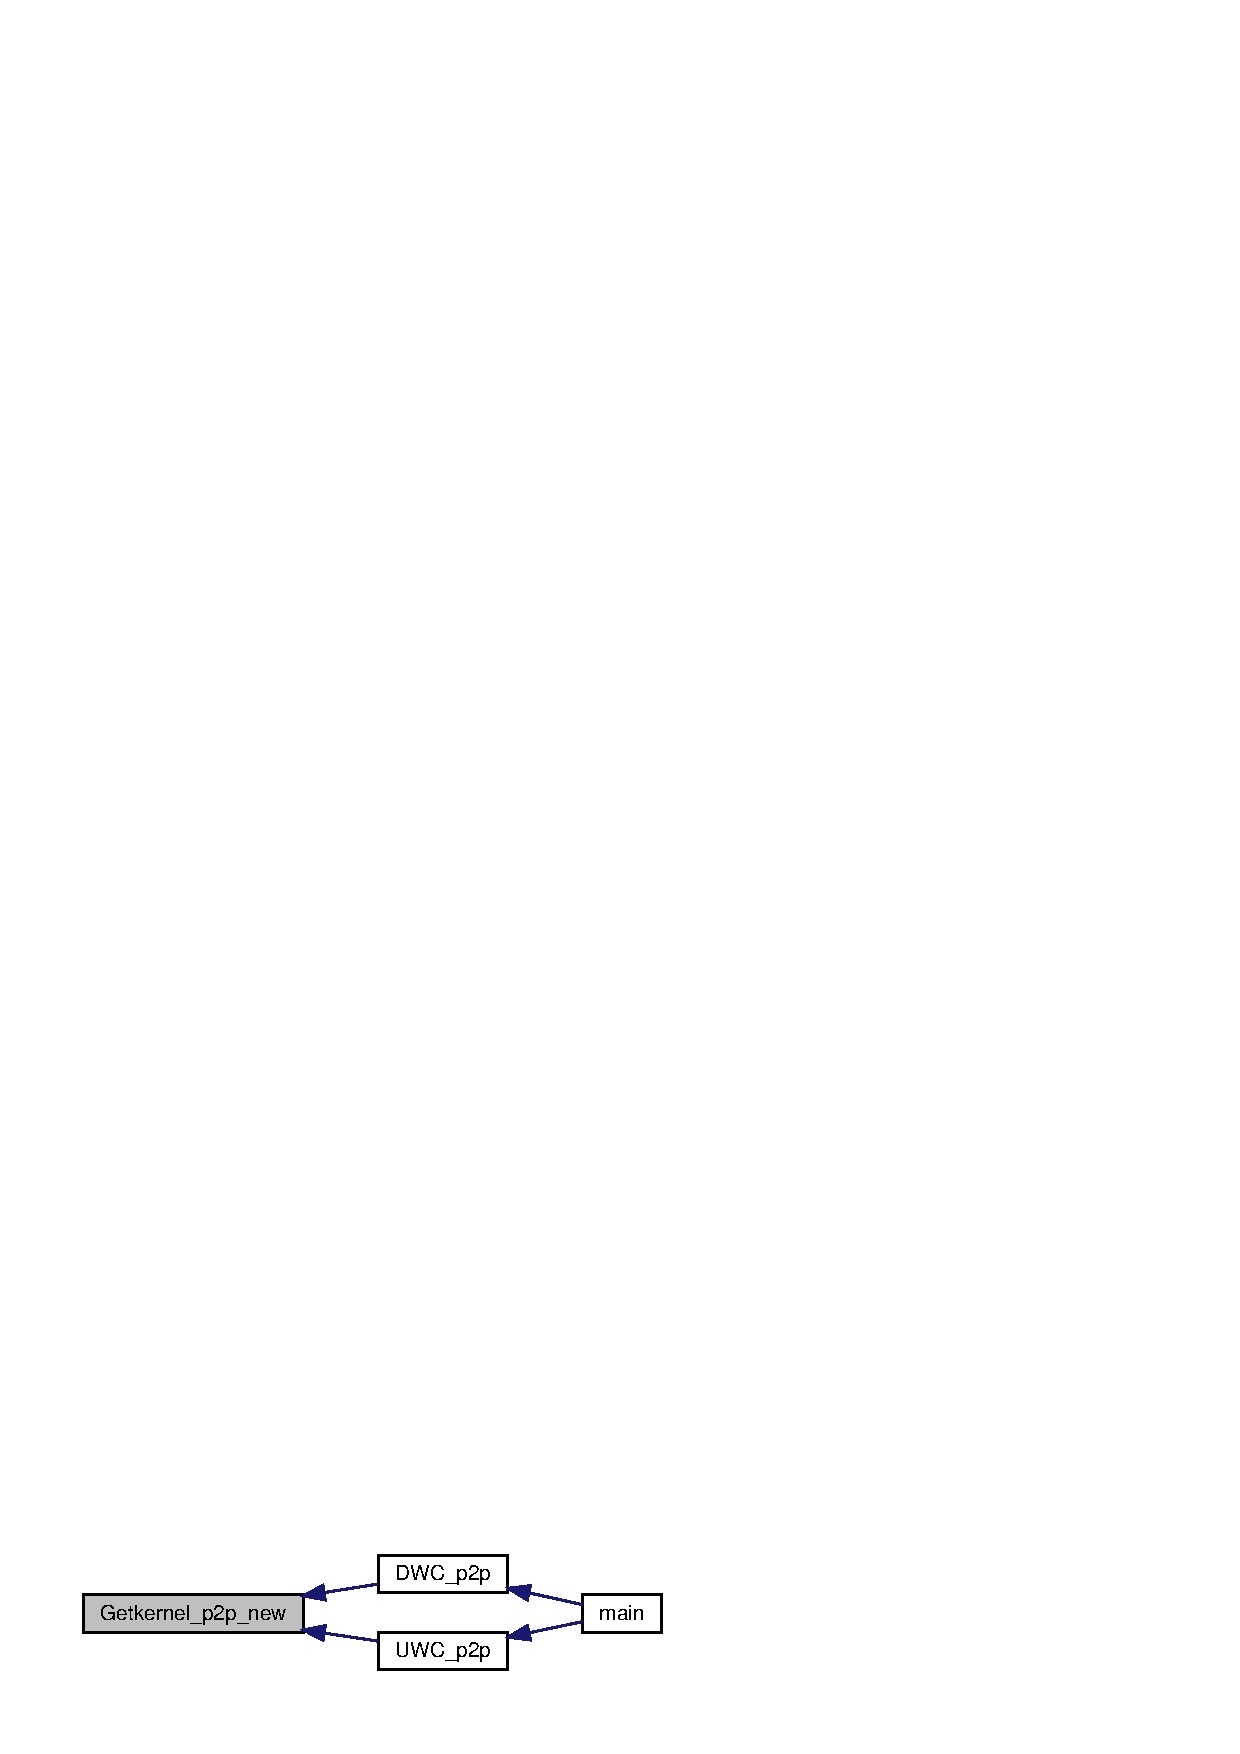
\includegraphics[width=321pt]{Conti2D_8cpp_a6f44a06f2b4926f66481fccf277bea50_a6f44a06f2b4926f66481fccf277bea50_icgraph}
\end{center}
\end{figure}
\mbox{\label{Conti2D_8cpp_a1d72c3a10bd62305a91d64bb0de2b247_a1d72c3a10bd62305a91d64bb0de2b247}} 
\index{Conti2\+D.\+cpp@{Conti2\+D.\+cpp}!Getkernel\+\_\+p2p\+\_\+new@{Getkernel\+\_\+p2p\+\_\+new}}
\index{Getkernel\+\_\+p2p\+\_\+new@{Getkernel\+\_\+p2p\+\_\+new}!Conti2\+D.\+cpp@{Conti2\+D.\+cpp}}
\subsubsection{Getkernel\+\_\+p2p\+\_\+new()\hspace{0.1cm}{\footnotesize\ttfamily [2/2]}}
{\footnotesize\ttfamily int Getkernel\+\_\+p2p\+\_\+new (\begin{DoxyParamCaption}\item[{\textbf{ Grd\+Head}}]{grdhead,  }\item[{double}]{rph,  }\item[{double $\ast$}]{kernel\+\_\+first\+Row,  }\item[{int}]{num\+\_\+thread }\end{DoxyParamCaption})}



Definition at line 305 of file Conti2\+D.\+cpp.



References Grd\+Head\+::bounds, Grd\+Head\+::cols, Get\+Pmnij(), and Grd\+Head\+::rows.

Here is the call graph for this function\+:\nopagebreak
\begin{figure}[H]
\begin{center}
\leavevmode
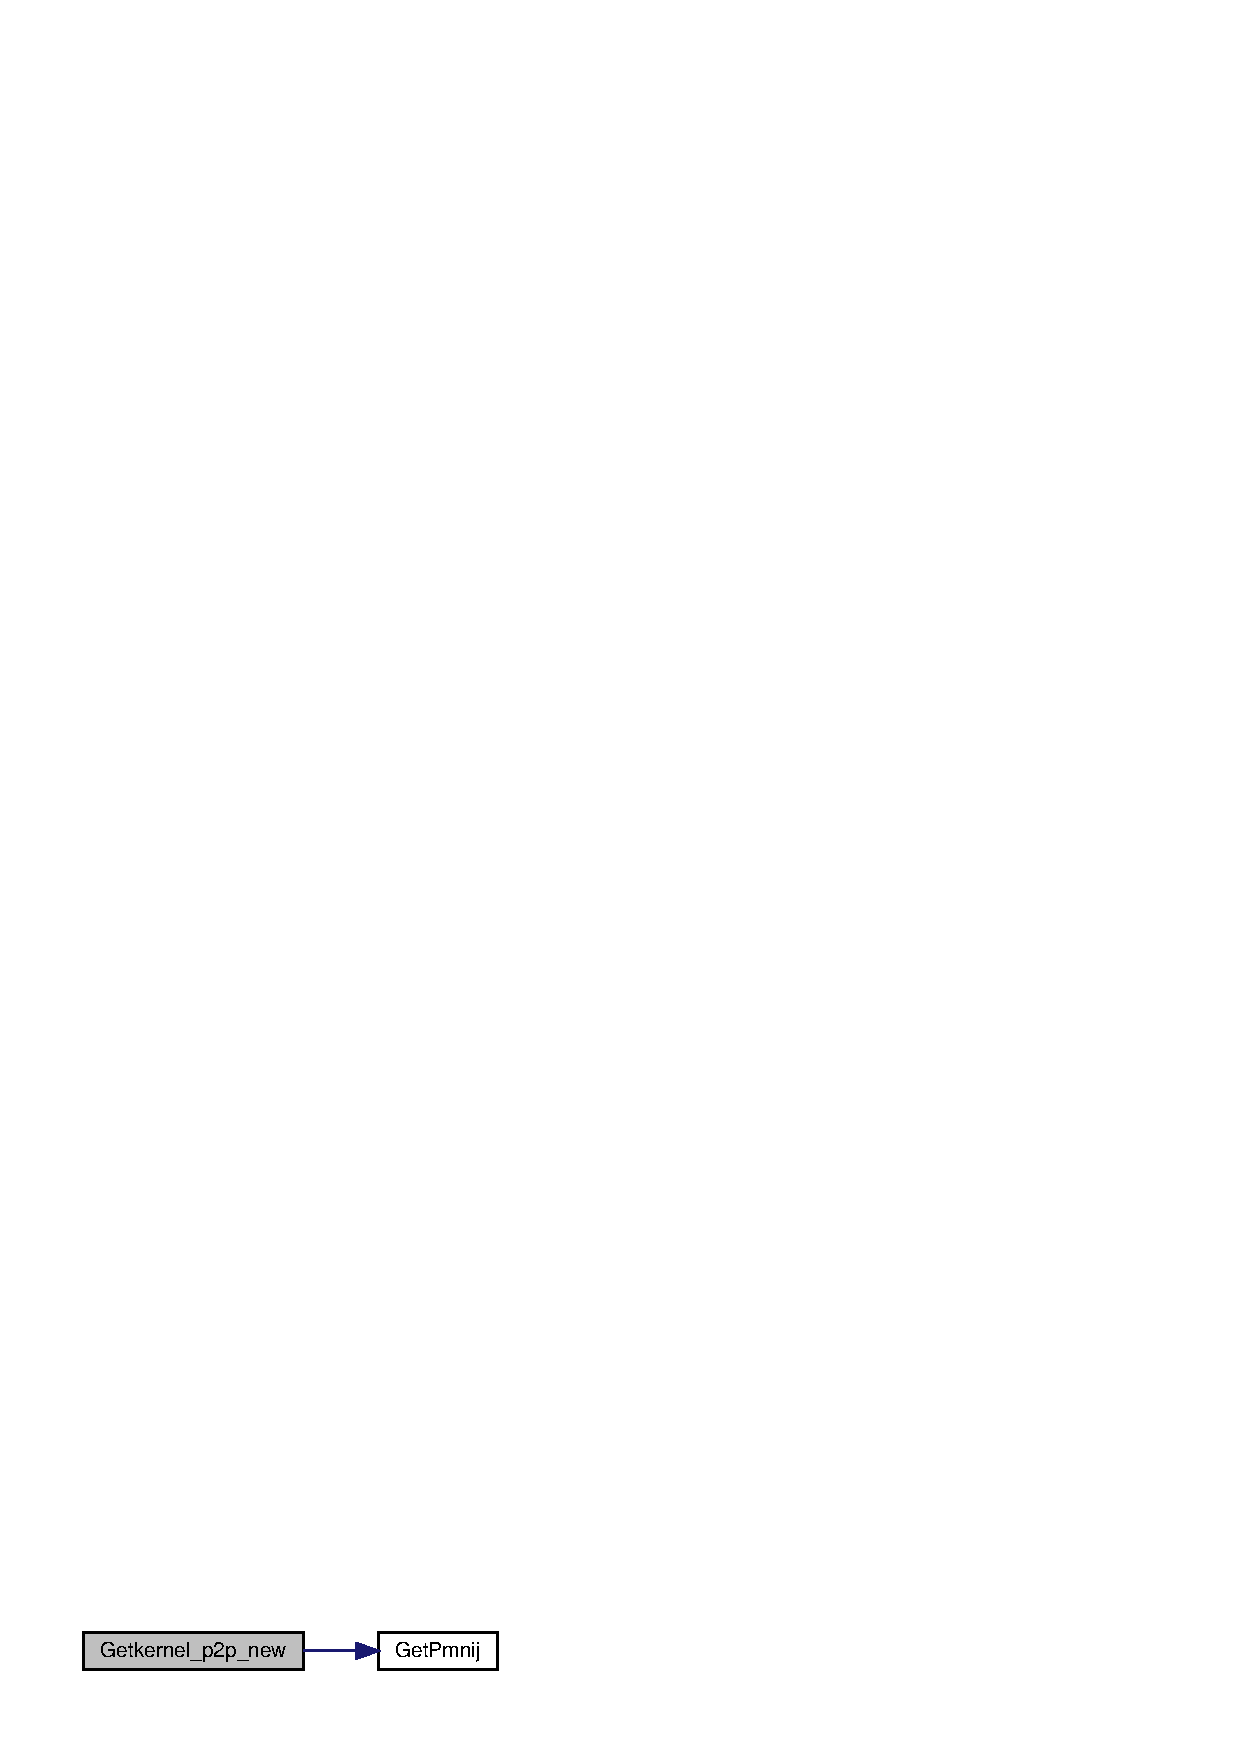
\includegraphics[width=243pt]{Conti2D_8cpp_a1d72c3a10bd62305a91d64bb0de2b247_a1d72c3a10bd62305a91d64bb0de2b247_cgraph}
\end{center}
\end{figure}
\mbox{\label{Conti2D_8cpp_a78d8a6b80166f8976a0f18caddbe1dcb_a78d8a6b80166f8976a0f18caddbe1dcb}} 
\index{Conti2\+D.\+cpp@{Conti2\+D.\+cpp}!Getkernel\+\_\+p2s\+\_\+new@{Getkernel\+\_\+p2s\+\_\+new}}
\index{Getkernel\+\_\+p2s\+\_\+new@{Getkernel\+\_\+p2s\+\_\+new}!Conti2\+D.\+cpp@{Conti2\+D.\+cpp}}
\subsubsection{Getkernel\+\_\+p2s\+\_\+new()}
{\footnotesize\ttfamily int Getkernel\+\_\+p2s\+\_\+new (\begin{DoxyParamCaption}\item[{\textbf{ Grd\+Head}}]{grdhead,  }\item[{double}]{h1,  }\item[{double $\ast$}]{topo2,  }\item[{double $\ast$$\ast$}]{kernel,  }\item[{int}]{num\+\_\+thread }\end{DoxyParamCaption})}



Definition at line 237 of file Conti2\+D.\+cpp.



References Grd\+Head\+::bounds, C\+O\+L\+O\+R\+\_\+\+B\+A\+R\+\_\+\+B\+L\+UE, Grd\+Head\+::cols, Get\+Pmnij(), Grd\+Head\+::rows, and Multi\+Progress\+Bar\+::\+Update().



Referenced by D\+W\+C\+\_\+s2p(), and U\+W\+C\+\_\+p2s().

Here is the call graph for this function\+:\nopagebreak
\begin{figure}[H]
\begin{center}
\leavevmode
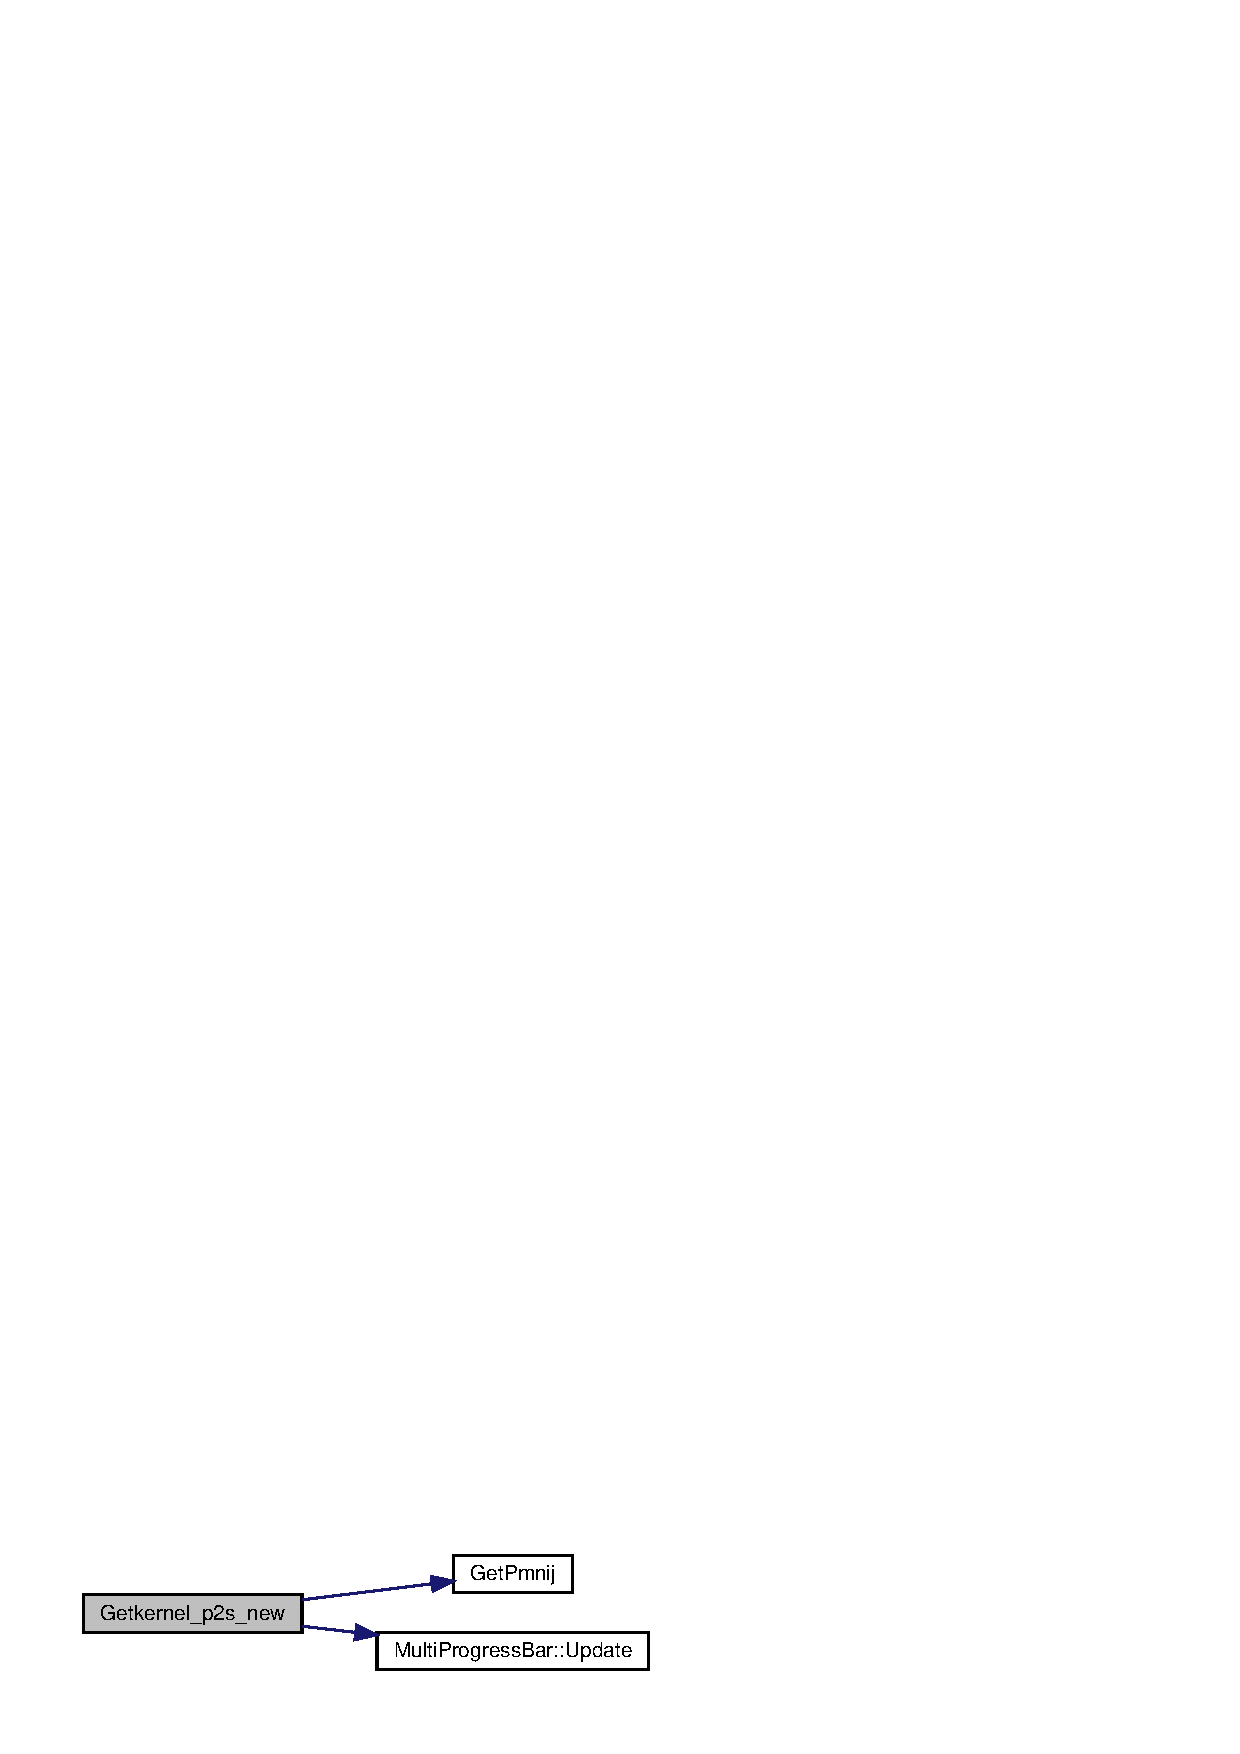
\includegraphics[width=315pt]{Conti2D_8cpp_a78d8a6b80166f8976a0f18caddbe1dcb_a78d8a6b80166f8976a0f18caddbe1dcb_cgraph}
\end{center}
\end{figure}
Here is the caller graph for this function\+:\nopagebreak
\begin{figure}[H]
\begin{center}
\leavevmode
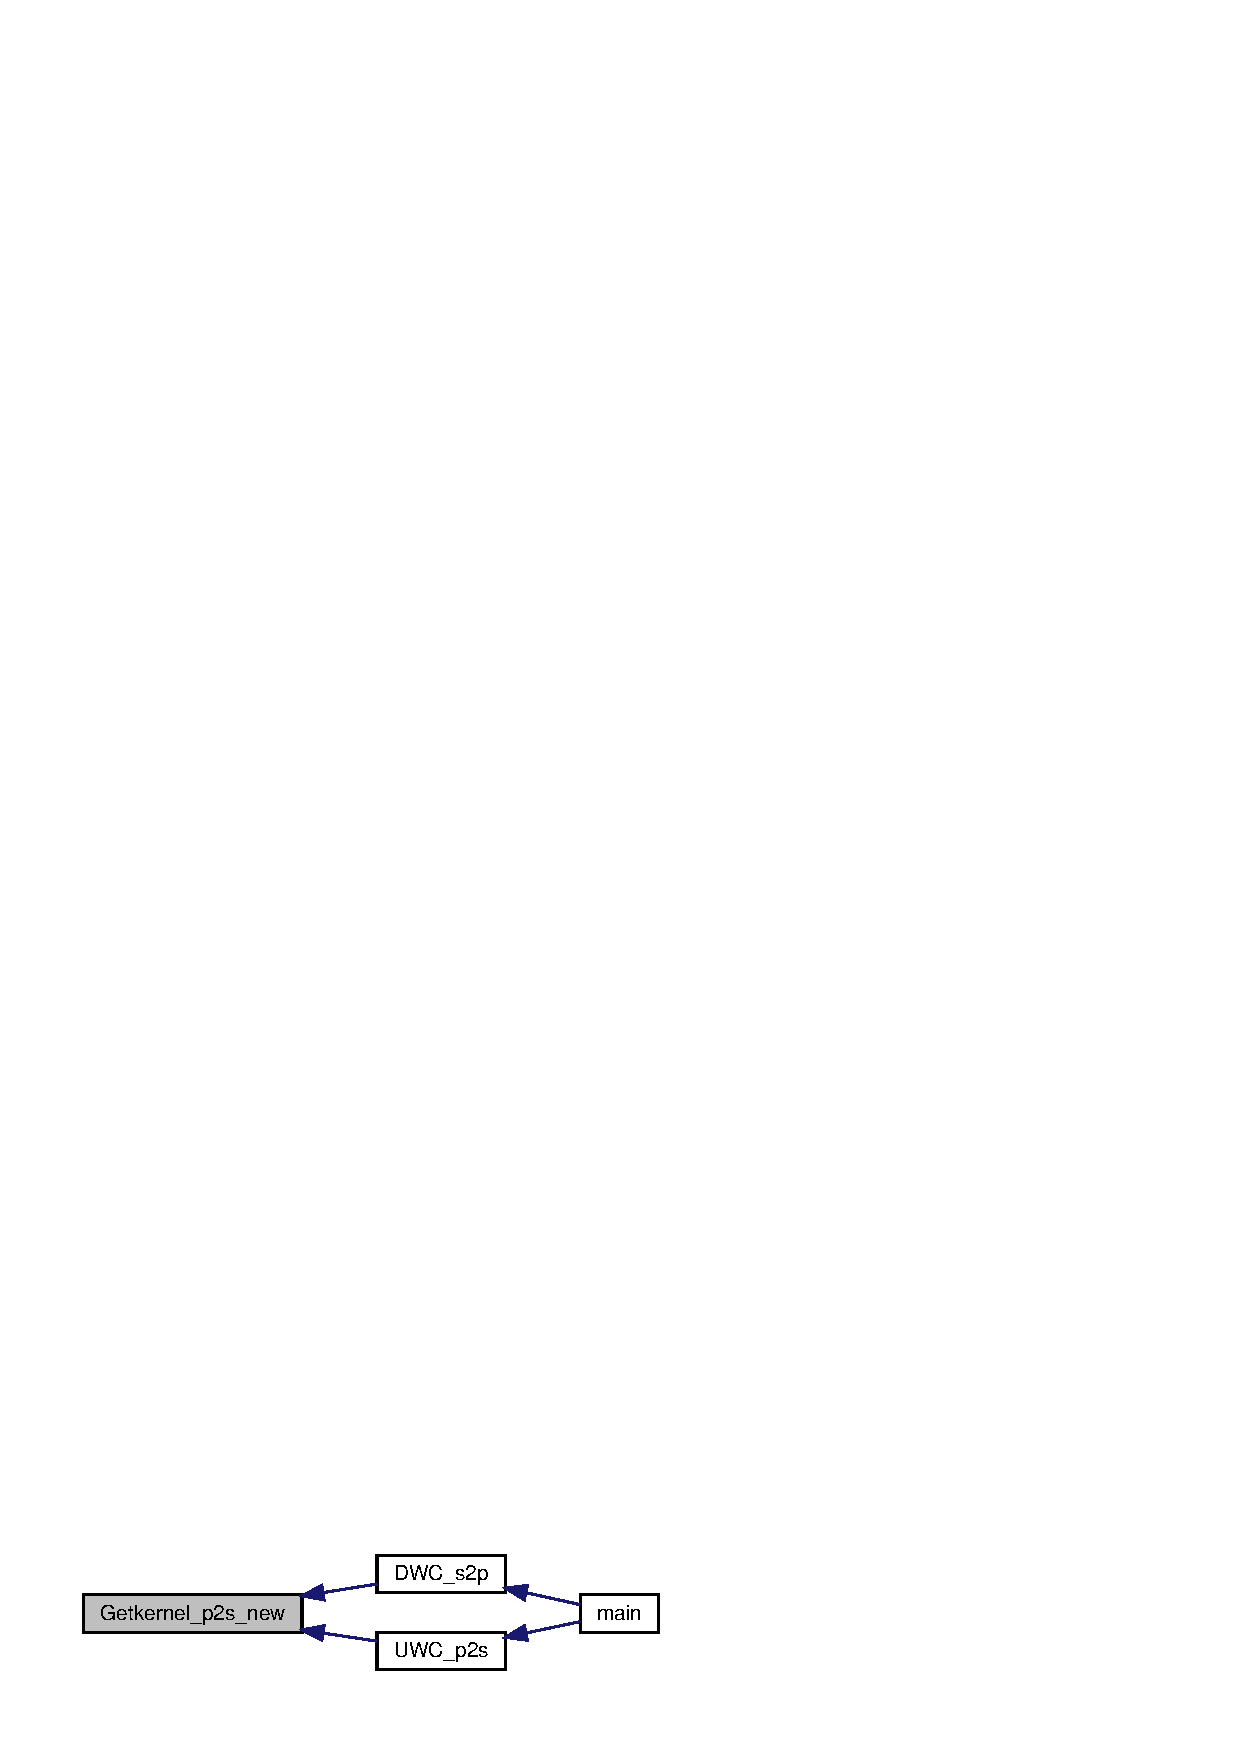
\includegraphics[width=320pt]{Conti2D_8cpp_a78d8a6b80166f8976a0f18caddbe1dcb_a78d8a6b80166f8976a0f18caddbe1dcb_icgraph}
\end{center}
\end{figure}
\mbox{\label{Conti2D_8cpp_a9b8597bfdb8429464d4453d41cbfb2d3_a9b8597bfdb8429464d4453d41cbfb2d3}} 
\index{Conti2\+D.\+cpp@{Conti2\+D.\+cpp}!Getkernel\+\_\+u2p@{Getkernel\+\_\+u2p}}
\index{Getkernel\+\_\+u2p@{Getkernel\+\_\+u2p}!Conti2\+D.\+cpp@{Conti2\+D.\+cpp}}
\subsubsection{Getkernel\+\_\+u2p()}
{\footnotesize\ttfamily int Getkernel\+\_\+u2p (\begin{DoxyParamCaption}\item[{\textbf{ Grd\+Head}}]{grdhead,  }\item[{double $\ast$}]{terrain1,  }\item[{double}]{height2,  }\item[{double $\ast$$\ast$}]{kernel,  }\item[{int}]{num\+\_\+thread }\end{DoxyParamCaption})}



Definition at line 584 of file Conti2\+D.\+cpp.



References Grd\+Head\+::bounds, Grd\+Head\+::cols, PI, and Grd\+Head\+::rows.

\mbox{\label{Conti2D_8cpp_aa99f45e33c5a1a8c605bbd31056347c7_aa99f45e33c5a1a8c605bbd31056347c7}} 
\index{Conti2\+D.\+cpp@{Conti2\+D.\+cpp}!Getkernel\+\_\+u2p\+\_\+new@{Getkernel\+\_\+u2p\+\_\+new}}
\index{Getkernel\+\_\+u2p\+\_\+new@{Getkernel\+\_\+u2p\+\_\+new}!Conti2\+D.\+cpp@{Conti2\+D.\+cpp}}
\subsubsection{Getkernel\+\_\+u2p\+\_\+new()}
{\footnotesize\ttfamily int Getkernel\+\_\+u2p\+\_\+new (\begin{DoxyParamCaption}\item[{\textbf{ Grd\+Head}}]{grdhead,  }\item[{double $\ast$}]{terrain1,  }\item[{double}]{height2,  }\item[{double $\ast$}]{nx,  }\item[{double $\ast$}]{ny,  }\item[{double $\ast$}]{nz,  }\item[{double $\ast$$\ast$}]{kernel,  }\item[{int}]{num\+\_\+thread }\end{DoxyParamCaption})}



Definition at line 626 of file Conti2\+D.\+cpp.



References Grd\+Head\+::bounds, Grd\+Head\+::cols, PI, and Grd\+Head\+::rows.

\mbox{\label{Conti2D_8cpp_a4bb34ae88cf16e429505f9eb746384cd_a4bb34ae88cf16e429505f9eb746384cd}} 
\index{Conti2\+D.\+cpp@{Conti2\+D.\+cpp}!Get\+Pmnij@{Get\+Pmnij}}
\index{Get\+Pmnij@{Get\+Pmnij}!Conti2\+D.\+cpp@{Conti2\+D.\+cpp}}
\subsubsection{Get\+Pmnij()}
{\footnotesize\ttfamily void Get\+Pmnij (\begin{DoxyParamCaption}\item[{double $\ast$}]{Pmnij,  }\item[{int}]{rows,  }\item[{int}]{cols,  }\item[{double}]{dx,  }\item[{double}]{dy,  }\item[{double}]{rph,  }\item[{double}]{xm,  }\item[{double}]{ym }\end{DoxyParamCaption})}



Definition at line 157 of file Conti2\+D.\+cpp.



References PI.



Referenced by Getkernel\+\_\+p2p\+\_\+new(), and Getkernel\+\_\+p2s\+\_\+new().

Here is the caller graph for this function\+:\nopagebreak
\begin{figure}[H]
\begin{center}
\leavevmode
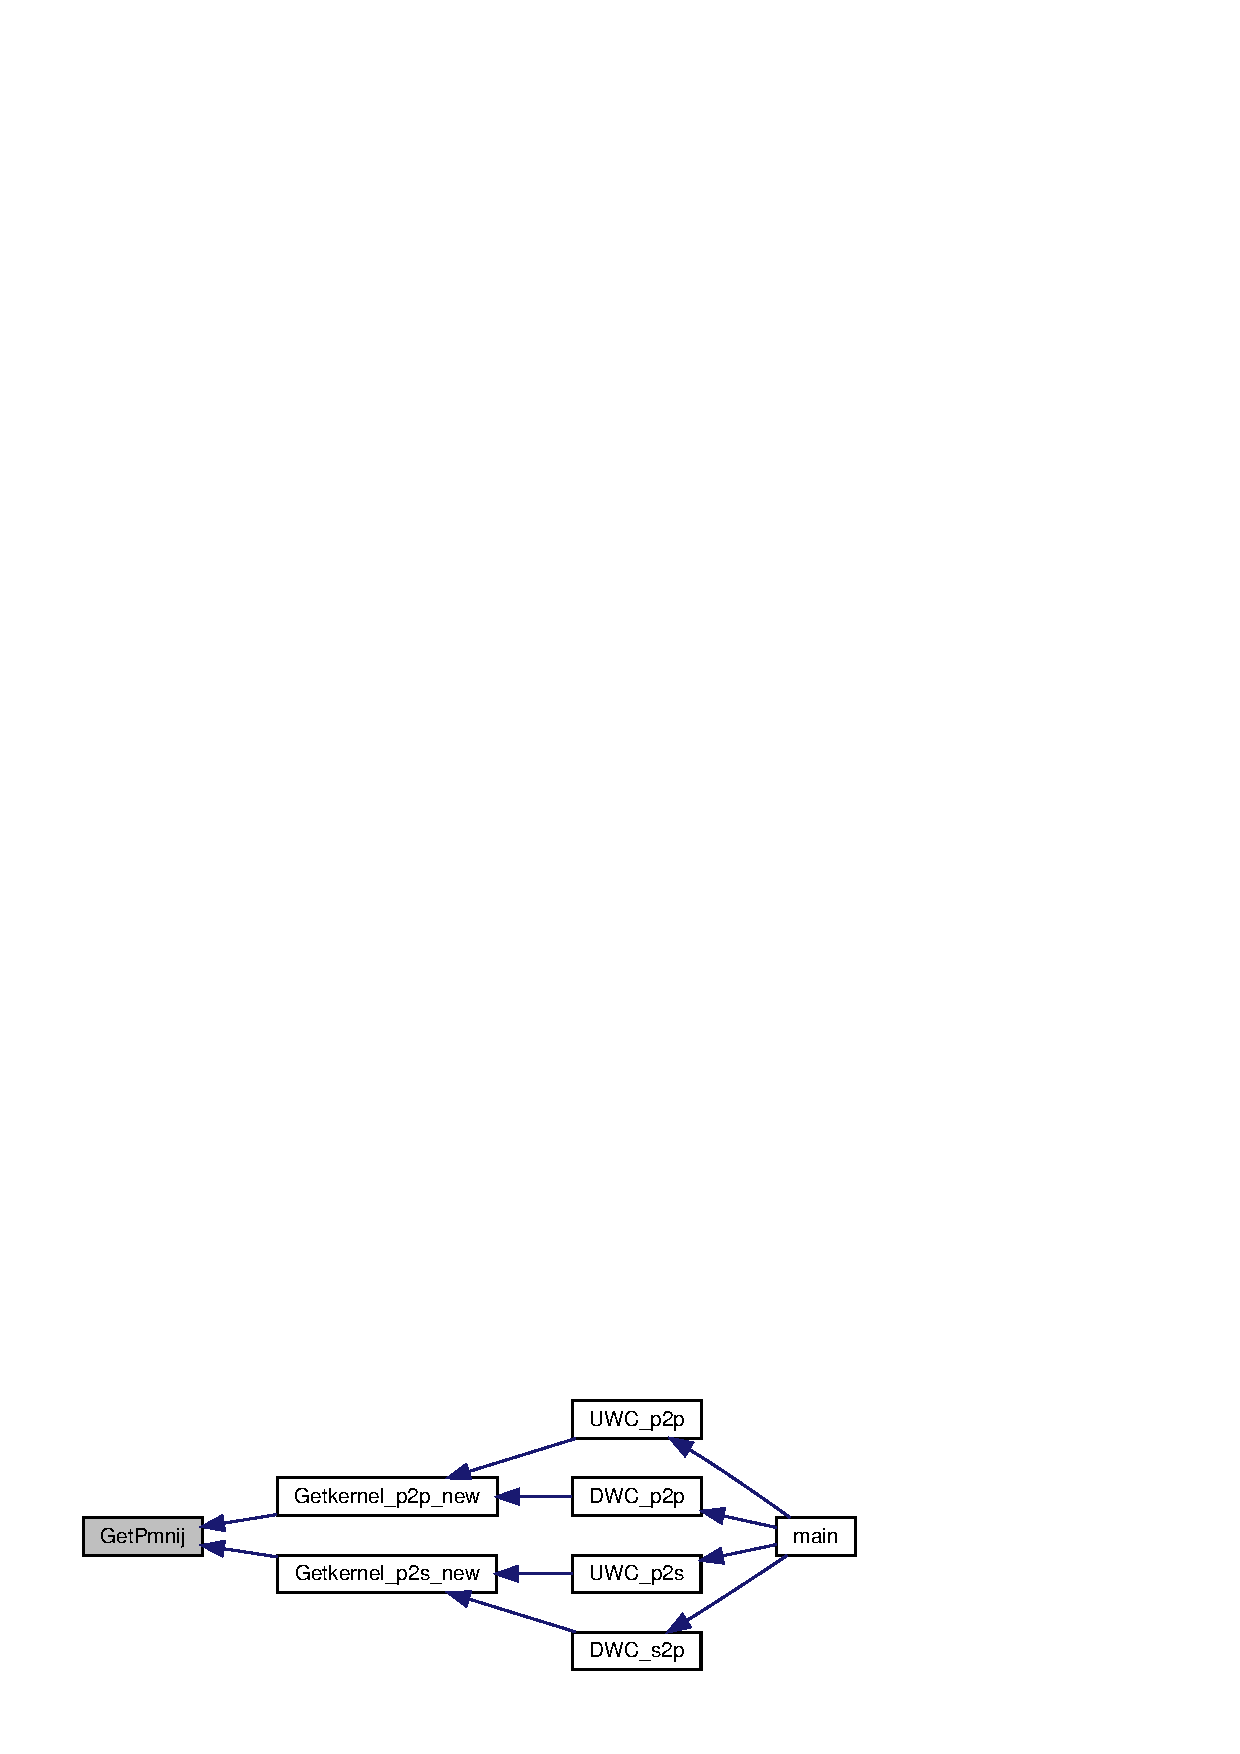
\includegraphics[width=350pt]{Conti2D_8cpp_a4bb34ae88cf16e429505f9eb746384cd_a4bb34ae88cf16e429505f9eb746384cd_icgraph}
\end{center}
\end{figure}
\mbox{\label{Conti2D_8cpp_a98827c14ed7072c96834f20205c7a916_a98827c14ed7072c96834f20205c7a916}} 
\index{Conti2\+D.\+cpp@{Conti2\+D.\+cpp}!Norm2@{Norm2}}
\index{Norm2@{Norm2}!Conti2\+D.\+cpp@{Conti2\+D.\+cpp}}
\subsubsection{Norm2()}
{\footnotesize\ttfamily double Norm2 (\begin{DoxyParamCaption}\item[{double $\ast$}]{x,  }\item[{const int}]{num }\end{DoxyParamCaption})}



Definition at line 2167 of file Conti2\+D.\+cpp.



Referenced by D\+W\+C\+\_\+p2p\+\_\+\+C\+G\+L\+S(), D\+W\+C\+\_\+p2p\+\_\+\+Itegration\+Iter(), D\+W\+C\+\_\+p2p\+\_\+\+Landweber\+Iter(), D\+W\+C\+\_\+s2p\+\_\+\+C\+G\+L\+S(), D\+W\+C\+\_\+s2p\+\_\+\+Itegration\+Iter(), D\+W\+C\+\_\+s2p\+\_\+\+Landweber\+Iter(), and D\+W\+C\+\_\+s2p\+\_\+\+Tikhonov().

Here is the caller graph for this function\+:\nopagebreak
\begin{figure}[H]
\begin{center}
\leavevmode
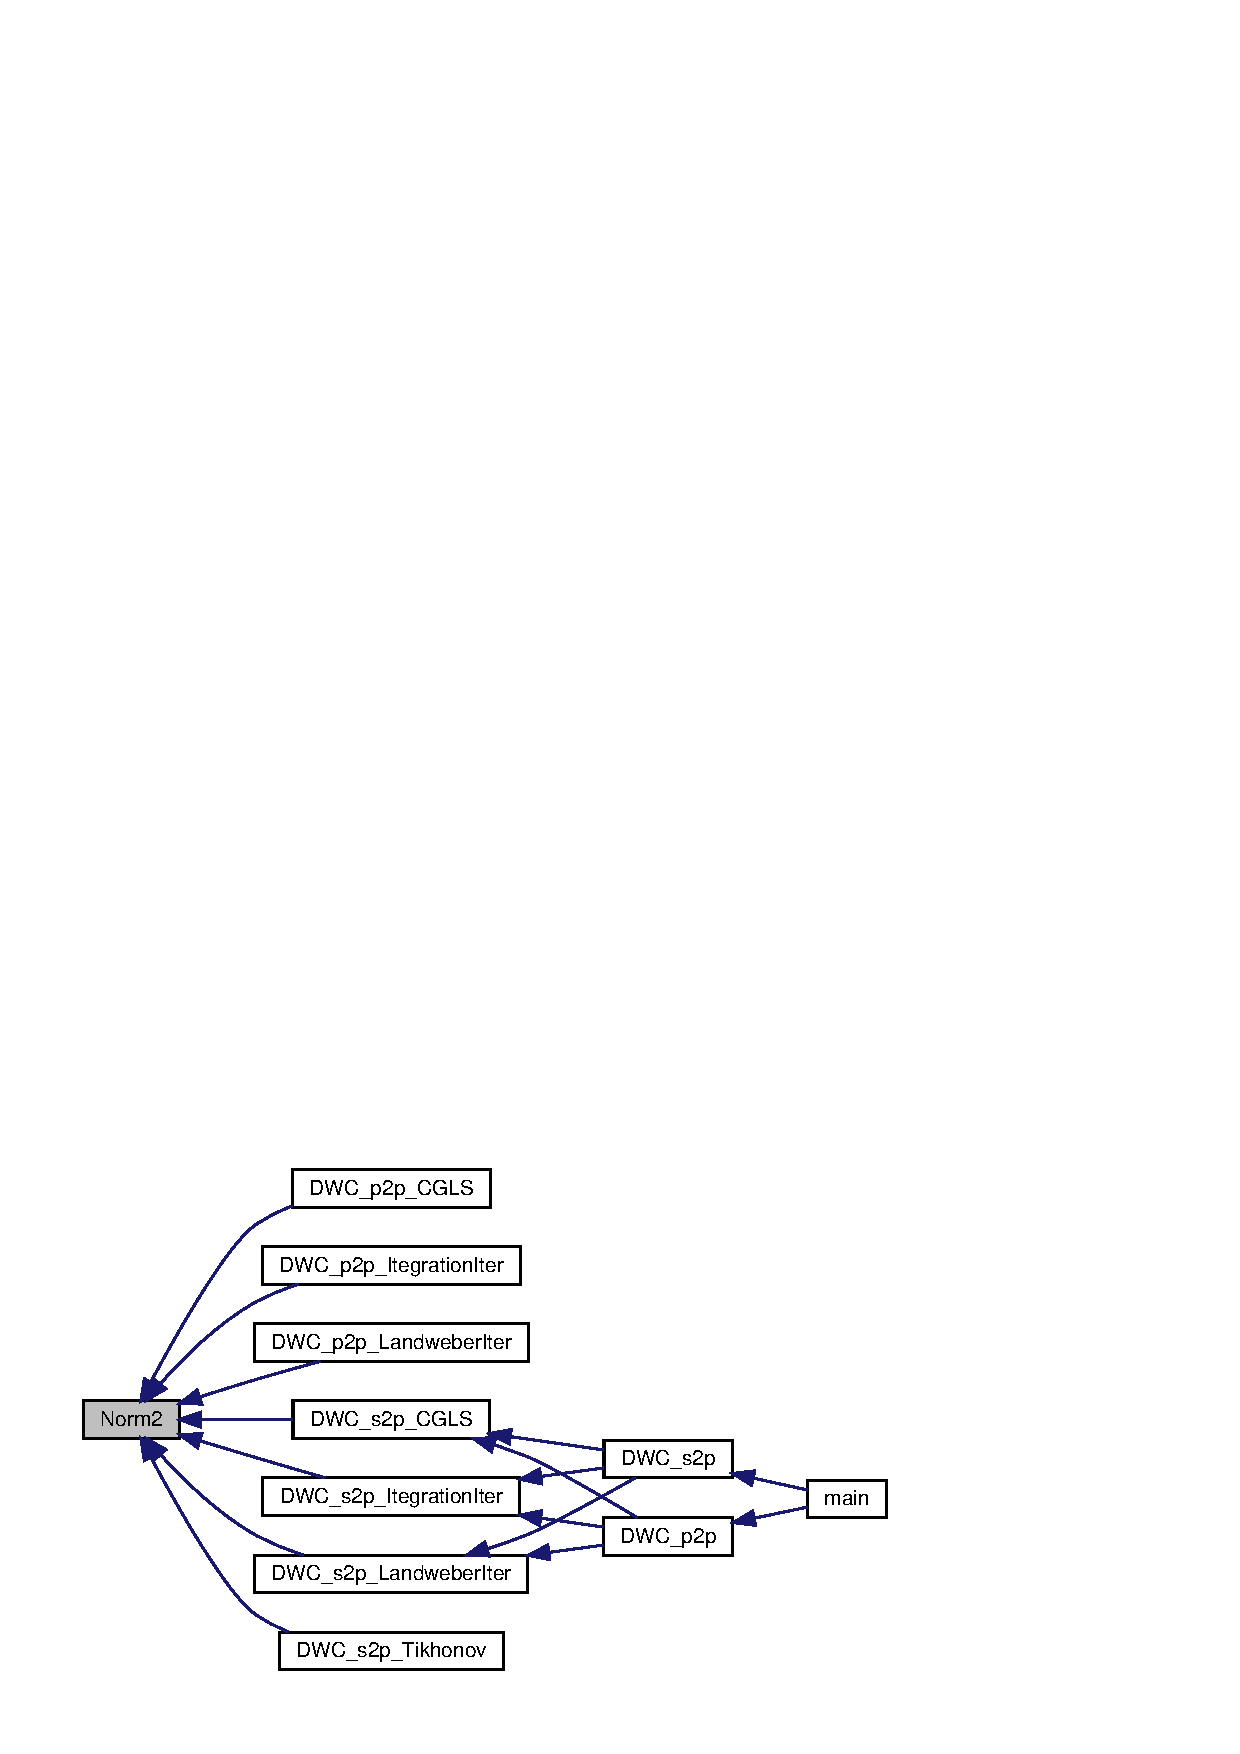
\includegraphics[width=350pt]{Conti2D_8cpp_a98827c14ed7072c96834f20205c7a916_a98827c14ed7072c96834f20205c7a916_icgraph}
\end{center}
\end{figure}
\mbox{\label{Conti2D_8cpp_a43fc3af75243a047d61aadea31c0fa9c_a43fc3af75243a047d61aadea31c0fa9c}} 
\index{Conti2\+D.\+cpp@{Conti2\+D.\+cpp}!Norm2\+\_\+\+Gradient@{Norm2\+\_\+\+Gradient}}
\index{Norm2\+\_\+\+Gradient@{Norm2\+\_\+\+Gradient}!Conti2\+D.\+cpp@{Conti2\+D.\+cpp}}
\subsubsection{Norm2\+\_\+\+Gradient()}
{\footnotesize\ttfamily double Norm2\+\_\+\+Gradient (\begin{DoxyParamCaption}\item[{double $\ast$}]{result,  }\item[{\textbf{ Grd\+Head}}]{grdhead }\end{DoxyParamCaption})}



Definition at line 2176 of file Conti2\+D.\+cpp.



References Grd\+Head\+::cols, and Grd\+Head\+::rows.



Referenced by D\+W\+C\+\_\+p2p\+\_\+\+Itegration\+Iter(), D\+W\+C\+\_\+p2p\+\_\+\+Landweber\+Iter(), D\+W\+C\+\_\+s2p\+\_\+\+Itegration\+Iter(), and D\+W\+C\+\_\+s2p\+\_\+\+Landweber\+Iter().

Here is the caller graph for this function\+:\nopagebreak
\begin{figure}[H]
\begin{center}
\leavevmode
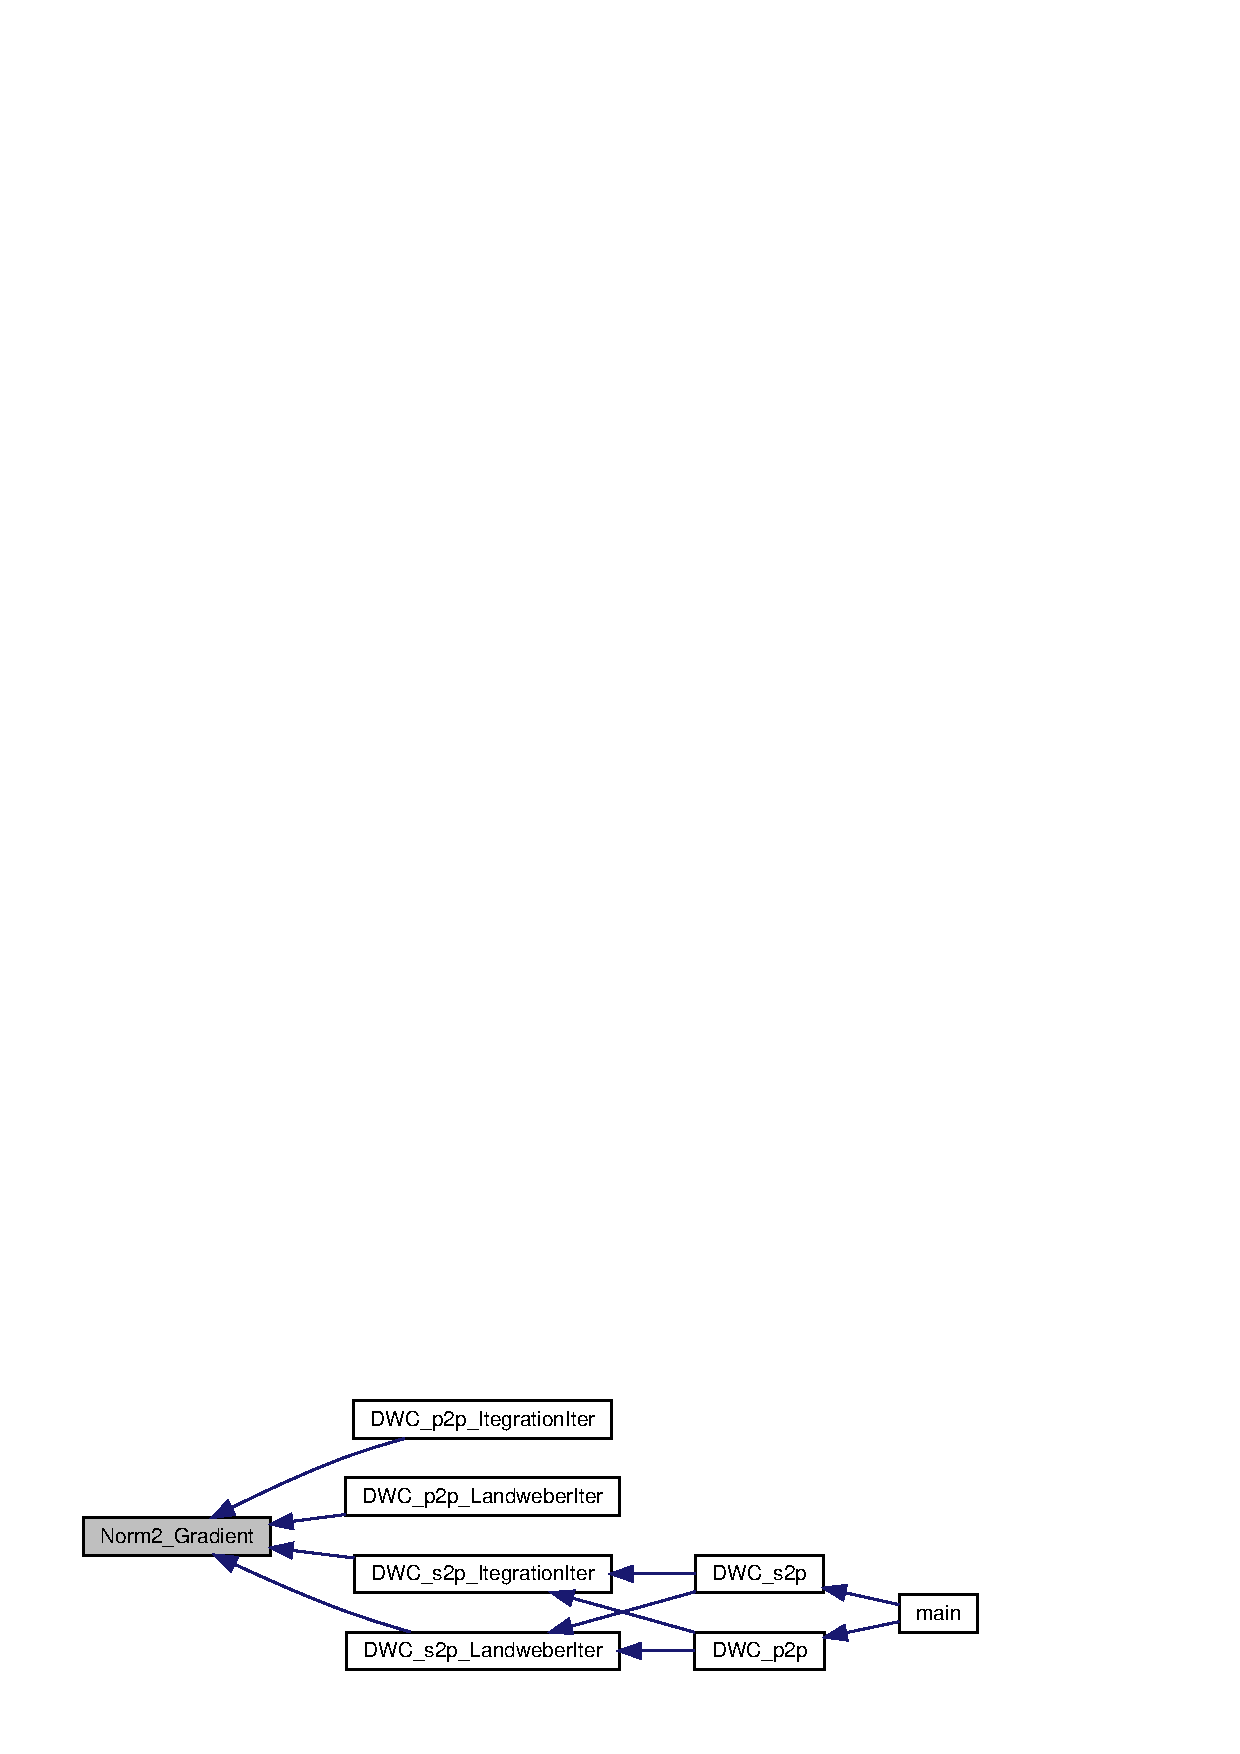
\includegraphics[width=350pt]{Conti2D_8cpp_a43fc3af75243a047d61aadea31c0fa9c_a43fc3af75243a047d61aadea31c0fa9c_icgraph}
\end{center}
\end{figure}
\mbox{\label{Conti2D_8cpp_a3c05f14aad4d9edc8c97ce180341a758_a3c05f14aad4d9edc8c97ce180341a758}} 
\index{Conti2\+D.\+cpp@{Conti2\+D.\+cpp}!Path\+\_\+\+Get\+Base\+Name@{Path\+\_\+\+Get\+Base\+Name}}
\index{Path\+\_\+\+Get\+Base\+Name@{Path\+\_\+\+Get\+Base\+Name}!Conti2\+D.\+cpp@{Conti2\+D.\+cpp}}
\subsubsection{Path\+\_\+\+Get\+Base\+Name()}
{\footnotesize\ttfamily string Path\+\_\+\+Get\+Base\+Name (\begin{DoxyParamCaption}\item[{string}]{filepath }\end{DoxyParamCaption})}



Definition at line 23 of file Conti2\+D.\+cpp.

\mbox{\label{Conti2D_8cpp_aaea96ecea3031c19d3ef88f6f1590d4a_aaea96ecea3031c19d3ef88f6f1590d4a}} 
\index{Conti2\+D.\+cpp@{Conti2\+D.\+cpp}!Path\+\_\+\+Get\+Ext\+Name@{Path\+\_\+\+Get\+Ext\+Name}}
\index{Path\+\_\+\+Get\+Ext\+Name@{Path\+\_\+\+Get\+Ext\+Name}!Conti2\+D.\+cpp@{Conti2\+D.\+cpp}}
\subsubsection{Path\+\_\+\+Get\+Ext\+Name()}
{\footnotesize\ttfamily string Path\+\_\+\+Get\+Ext\+Name (\begin{DoxyParamCaption}\item[{string}]{filepath }\end{DoxyParamCaption})}



Definition at line 17 of file Conti2\+D.\+cpp.

\mbox{\label{Conti2D_8cpp_a88f10a86b8808047787d2df5e8cbcb72_a88f10a86b8808047787d2df5e8cbcb72}} 
\index{Conti2\+D.\+cpp@{Conti2\+D.\+cpp}!Path\+\_\+\+Get\+File\+Name@{Path\+\_\+\+Get\+File\+Name}}
\index{Path\+\_\+\+Get\+File\+Name@{Path\+\_\+\+Get\+File\+Name}!Conti2\+D.\+cpp@{Conti2\+D.\+cpp}}
\subsubsection{Path\+\_\+\+Get\+File\+Name()}
{\footnotesize\ttfamily string Path\+\_\+\+Get\+File\+Name (\begin{DoxyParamCaption}\item[{string}]{filepath }\end{DoxyParamCaption})}



Definition at line 5 of file Conti2\+D.\+cpp.



Referenced by D\+W\+C\+\_\+p2p\+\_\+\+Itegration\+Iter(), D\+W\+C\+\_\+p2p\+\_\+\+Landweber\+Iter(), D\+W\+C\+\_\+s2p\+\_\+\+Itegration\+Iter(), and D\+W\+C\+\_\+s2p\+\_\+\+Landweber\+Iter().

Here is the caller graph for this function\+:\nopagebreak
\begin{figure}[H]
\begin{center}
\leavevmode
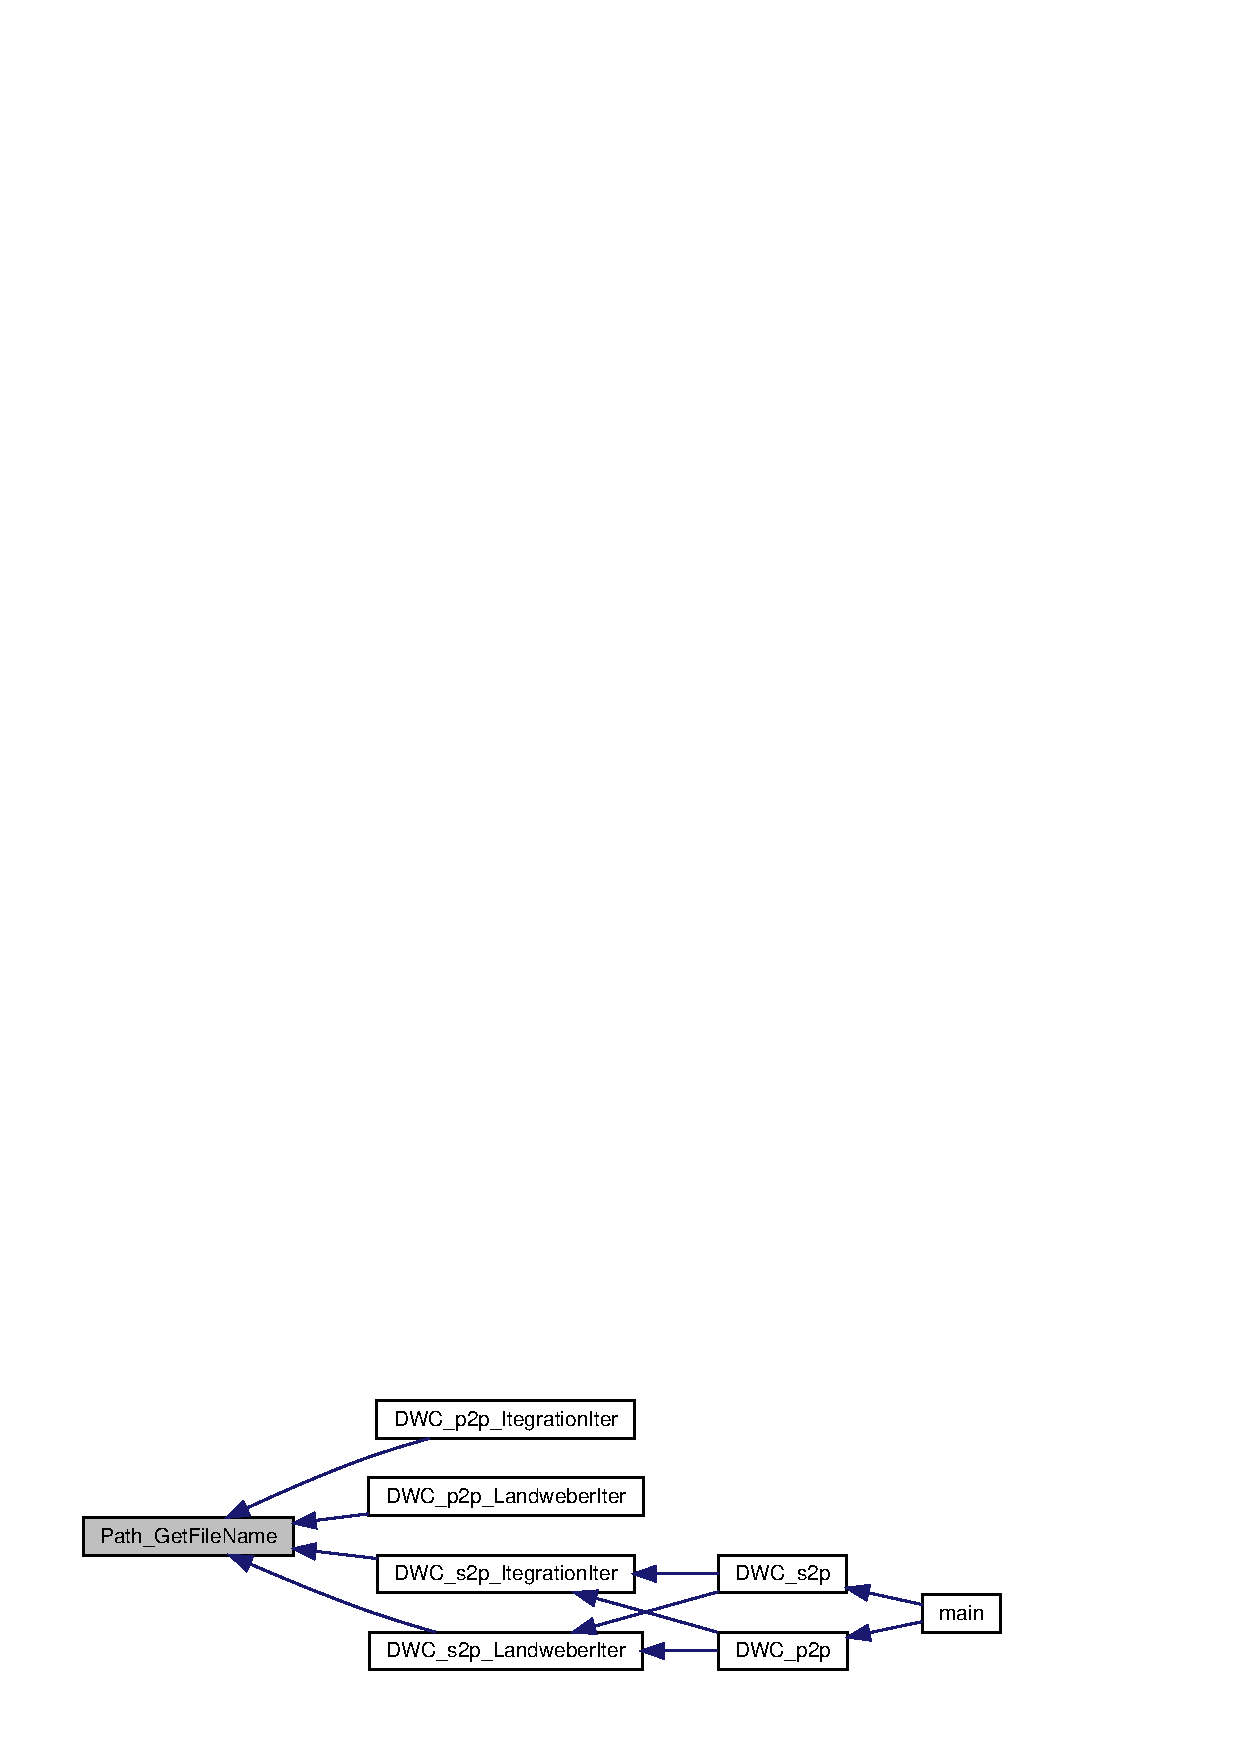
\includegraphics[width=350pt]{Conti2D_8cpp_a88f10a86b8808047787d2df5e8cbcb72_a88f10a86b8808047787d2df5e8cbcb72_icgraph}
\end{center}
\end{figure}
\mbox{\label{Conti2D_8cpp_acb5dfc7e5499641f231021a61660b0b7_acb5dfc7e5499641f231021a61660b0b7}} 
\index{Conti2\+D.\+cpp@{Conti2\+D.\+cpp}!Path\+\_\+\+Get\+Path@{Path\+\_\+\+Get\+Path}}
\index{Path\+\_\+\+Get\+Path@{Path\+\_\+\+Get\+Path}!Conti2\+D.\+cpp@{Conti2\+D.\+cpp}}
\subsubsection{Path\+\_\+\+Get\+Path()}
{\footnotesize\ttfamily string Path\+\_\+\+Get\+Path (\begin{DoxyParamCaption}\item[{string}]{filepath }\end{DoxyParamCaption})}



Definition at line 11 of file Conti2\+D.\+cpp.

\mbox{\label{Conti2D_8cpp_a2c90cdea3ca11177ba34c14a3b0a00cb_a2c90cdea3ca11177ba34c14a3b0a00cb}} 
\index{Conti2\+D.\+cpp@{Conti2\+D.\+cpp}!Read\+Grd@{Read\+Grd}}
\index{Read\+Grd@{Read\+Grd}!Conti2\+D.\+cpp@{Conti2\+D.\+cpp}}
\subsubsection{Read\+Grd()}
{\footnotesize\ttfamily double$\ast$ Read\+Grd (\begin{DoxyParamCaption}\item[{string}]{filename,  }\item[{\textbf{ Grd\+Head} \&}]{grdhead,  }\item[{int}]{ext\+Num }\end{DoxyParamCaption})}



Read a Surfer Grid data from file. 


\begin{DoxyParams}{Parameters}
{\em filename} & \\
\hline
{\em grdhead} & \\
\hline
{\em ext\+Num} & \\
\hline
\end{DoxyParams}
\begin{DoxyReturn}{Returns}
double$\ast$ return data array 
\end{DoxyReturn}


Definition at line 721 of file Conti2\+D.\+cpp.



References B\+L\+UE, Grd\+Head\+::bounds, C\+O\+L\+O\+R\+\_\+\+D\+E\+F\+A\+L\+UT, Grd\+Head\+::cols, G\+R\+E\+EN, R\+ED, and Grd\+Head\+::rows.



Referenced by D\+W\+C\+\_\+p2p(), D\+W\+C\+\_\+p2p\+\_\+f(), D\+W\+C\+\_\+s2p(), U\+W\+C\+\_\+p2p(), U\+W\+C\+\_\+p2p\+\_\+f(), and U\+W\+C\+\_\+p2s().

Here is the caller graph for this function\+:\nopagebreak
\begin{figure}[H]
\begin{center}
\leavevmode
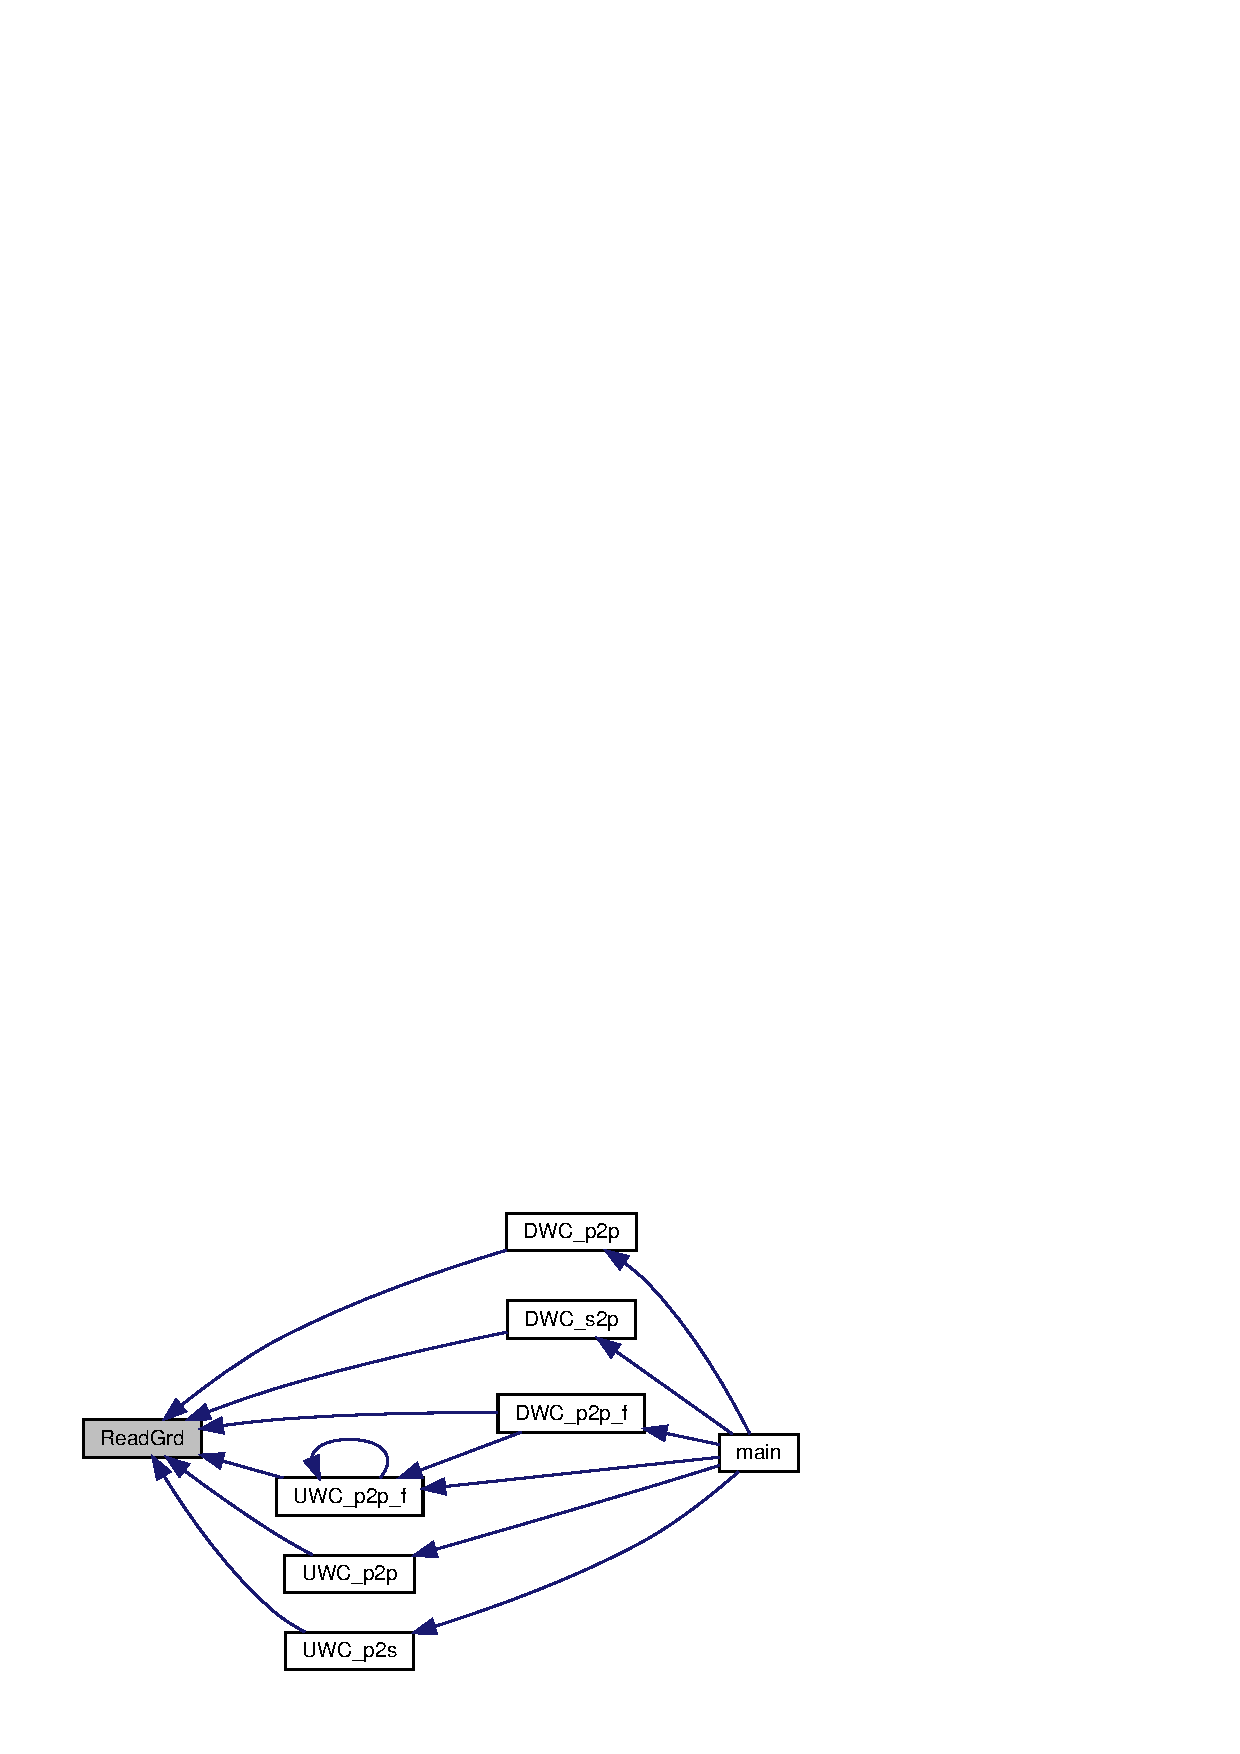
\includegraphics[width=350pt]{Conti2D_8cpp_a2c90cdea3ca11177ba34c14a3b0a00cb_a2c90cdea3ca11177ba34c14a3b0a00cb_icgraph}
\end{center}
\end{figure}
\mbox{\label{Conti2D_8cpp_ab76adf263893ac28772283c5a00b964c_ab76adf263893ac28772283c5a00b964c}} 
\index{Conti2\+D.\+cpp@{Conti2\+D.\+cpp}!Save\+Grd@{Save\+Grd}}
\index{Save\+Grd@{Save\+Grd}!Conti2\+D.\+cpp@{Conti2\+D.\+cpp}}
\subsubsection{Save\+Grd()}
{\footnotesize\ttfamily bool Save\+Grd (\begin{DoxyParamCaption}\item[{string}]{filename,  }\item[{\textbf{ Grd\+Head}}]{grdhead,  }\item[{double $\ast$}]{data,  }\item[{int}]{ext\+Num,  }\item[{bool}]{savexxyz = {\ttfamily false},  }\item[{bool}]{is\+Info = {\ttfamily true} }\end{DoxyParamCaption})}



Save a Surfer Grid data to file. 


\begin{DoxyParams}{Parameters}
{\em filename} & \\
\hline
{\em grdhead} & \\
\hline
{\em data} & \\
\hline
{\em ext\+Num} & \\
\hline
{\em savexxyz} & true\+: save xyz format simultaneously \\
\hline
{\em is\+Info} & \\
\hline
\end{DoxyParams}
\begin{DoxyReturn}{Returns}
true 

false 
\end{DoxyReturn}


Definition at line 808 of file Conti2\+D.\+cpp.



References Grd\+Head\+::bounds, C\+O\+L\+O\+R\+\_\+\+D\+E\+F\+A\+L\+UT, Grd\+Head\+::cols, G\+R\+E\+EN, and Grd\+Head\+::rows.



Referenced by D\+W\+C\+\_\+p2p(), D\+W\+C\+\_\+p2p\+\_\+\+C\+G\+L\+S(), D\+W\+C\+\_\+p2p\+\_\+f(), D\+W\+C\+\_\+p2p\+\_\+\+Itegration\+Iter(), D\+W\+C\+\_\+p2p\+\_\+\+Landweber\+Iter(), D\+W\+C\+\_\+s2p(), D\+W\+C\+\_\+s2p\+\_\+\+C\+G\+L\+S(), D\+W\+C\+\_\+s2p\+\_\+\+Itegration\+Iter(), D\+W\+C\+\_\+s2p\+\_\+\+Landweber\+Iter(), D\+W\+C\+\_\+s2p\+\_\+\+Tikhonov(), U\+W\+C\+\_\+p2p(), U\+W\+C\+\_\+p2p\+\_\+f(), and U\+W\+C\+\_\+p2s().

Here is the caller graph for this function\+:\nopagebreak
\begin{figure}[H]
\begin{center}
\leavevmode
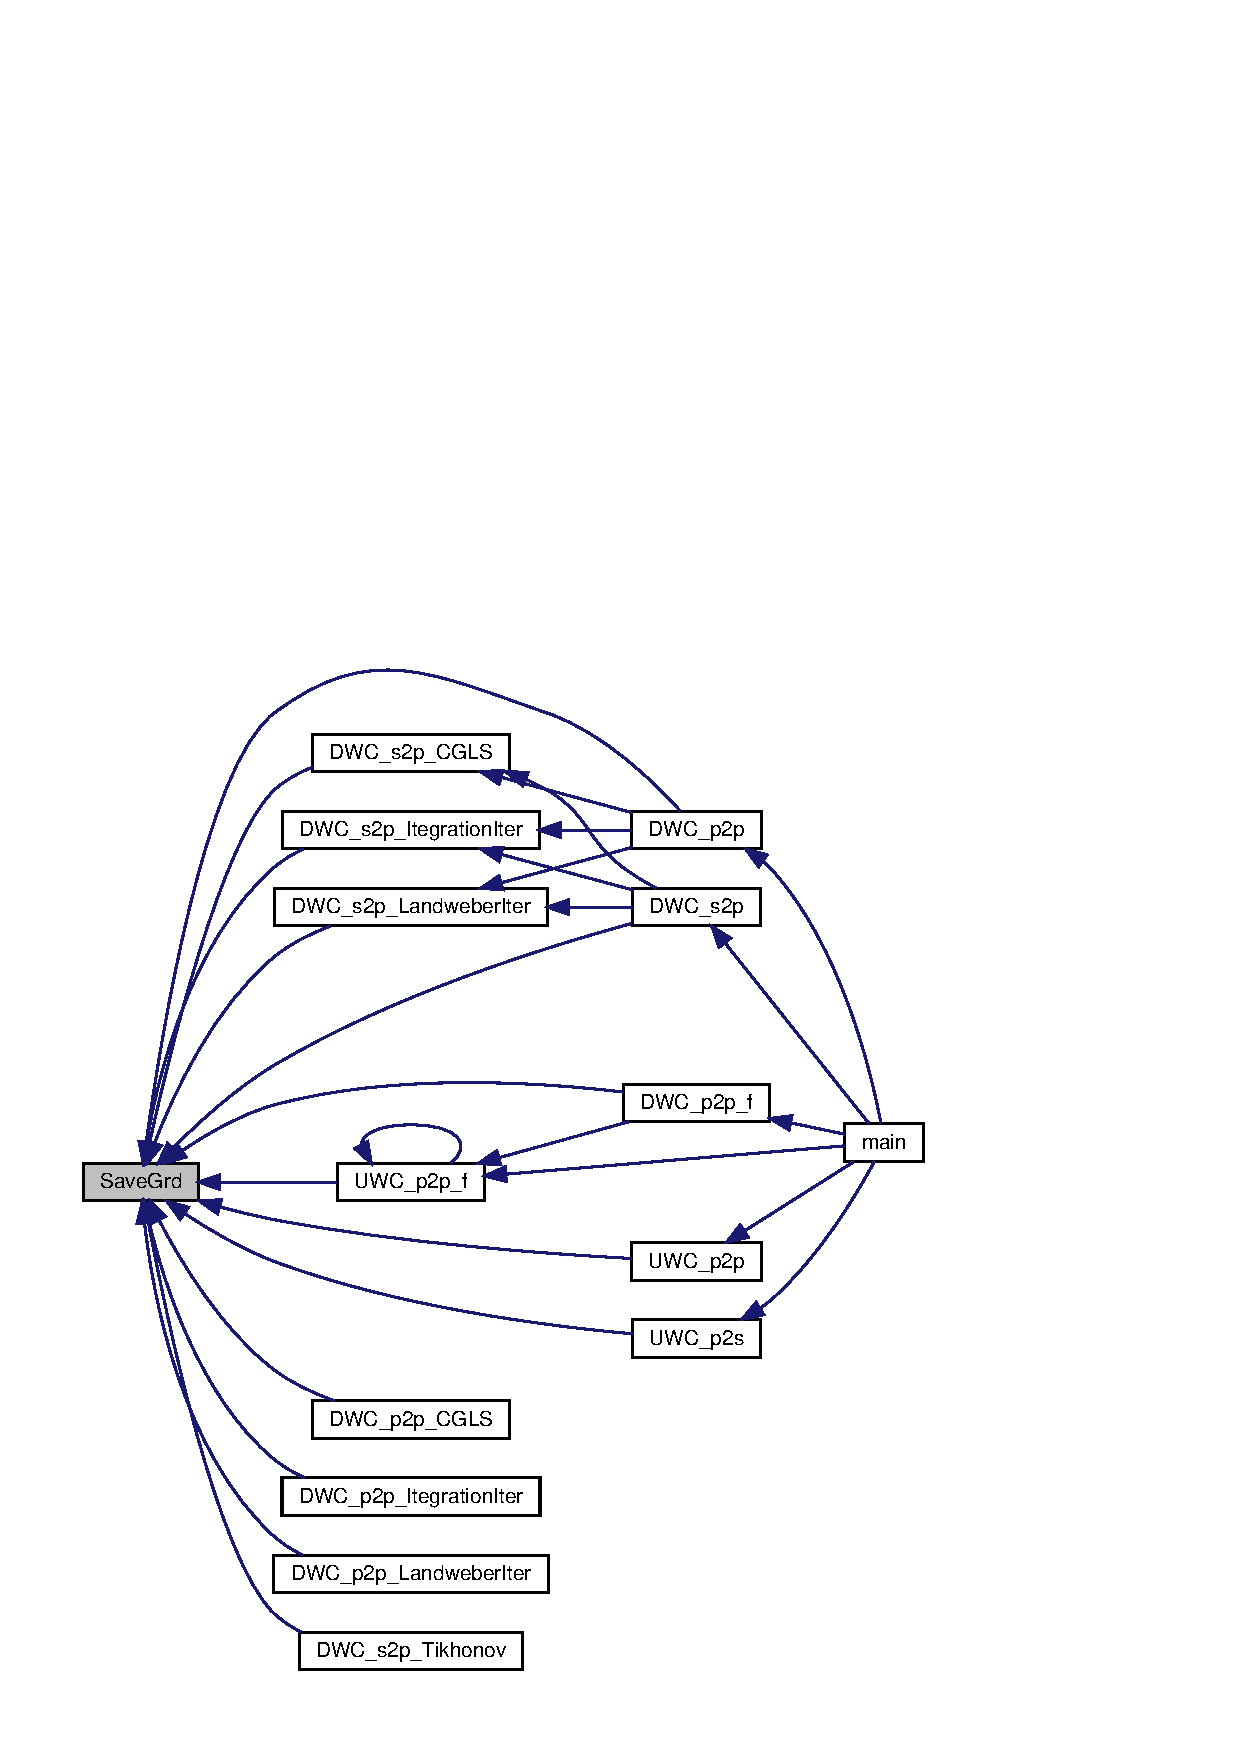
\includegraphics[width=350pt]{Conti2D_8cpp_ab76adf263893ac28772283c5a00b964c_ab76adf263893ac28772283c5a00b964c_icgraph}
\end{center}
\end{figure}
\mbox{\label{Conti2D_8cpp_ab2ce25b899be8dca564dd7dccde5e671_ab2ce25b899be8dca564dd7dccde5e671}} 
\index{Conti2\+D.\+cpp@{Conti2\+D.\+cpp}!Save\+Grd2\+V\+TK@{Save\+Grd2\+V\+TK}}
\index{Save\+Grd2\+V\+TK@{Save\+Grd2\+V\+TK}!Conti2\+D.\+cpp@{Conti2\+D.\+cpp}}
\subsubsection{Save\+Grd2\+V\+T\+K()}
{\footnotesize\ttfamily int Save\+Grd2\+V\+TK (\begin{DoxyParamCaption}\item[{string}]{outputfile,  }\item[{\textbf{ Grd\+Head}}]{grdhead,  }\item[{double $\ast$}]{data }\end{DoxyParamCaption})}



Definition at line 2213 of file Conti2\+D.\+cpp.



References Grd\+Head\+::bounds, C\+O\+L\+O\+R\+\_\+\+D\+E\+F\+A\+L\+UT, Grd\+Head\+::cols, R\+ED, and Grd\+Head\+::rows.

\mbox{\label{Conti2D_8cpp_a2418639857d09d54494ee0dc5fa8df78_a2418639857d09d54494ee0dc5fa8df78}} 
\index{Conti2\+D.\+cpp@{Conti2\+D.\+cpp}!U\+WC@{U\+WC}}
\index{U\+WC@{U\+WC}!Conti2\+D.\+cpp@{Conti2\+D.\+cpp}}
\subsubsection{U\+W\+C()}
{\footnotesize\ttfamily void U\+WC (\begin{DoxyParamCaption}\item[{double $\ast$}]{datain,  }\item[{double $\ast$}]{dataout,  }\item[{\textbf{ Grd\+Head}}]{grdhead,  }\item[{double $\ast$$\ast$}]{G }\end{DoxyParamCaption})}



Definition at line 954 of file Conti2\+D.\+cpp.



References Grd\+Head\+::cols, and Grd\+Head\+::rows.

\mbox{\label{Conti2D_8cpp_a6e44071dbbec5b92ddf8673dea8c41de_a6e44071dbbec5b92ddf8673dea8c41de}} 
\index{Conti2\+D.\+cpp@{Conti2\+D.\+cpp}!U\+W\+C\+\_\+\+G\+\_\+\+C\+G\+L\+S\+\_\+\+Tik@{U\+W\+C\+\_\+\+G\+\_\+\+C\+G\+L\+S\+\_\+\+Tik}}
\index{U\+W\+C\+\_\+\+G\+\_\+\+C\+G\+L\+S\+\_\+\+Tik@{U\+W\+C\+\_\+\+G\+\_\+\+C\+G\+L\+S\+\_\+\+Tik}!Conti2\+D.\+cpp@{Conti2\+D.\+cpp}}
\subsubsection{U\+W\+C\+\_\+\+G\+\_\+\+C\+G\+L\+S\+\_\+\+Tik()}
{\footnotesize\ttfamily void U\+W\+C\+\_\+\+G\+\_\+\+C\+G\+L\+S\+\_\+\+Tik (\begin{DoxyParamCaption}\item[{double $\ast$}]{b,  }\item[{double $\ast$$\ast$}]{G,  }\item[{double $\ast$}]{x,  }\item[{int}]{modelnum,  }\item[{double}]{lambda2,  }\item[{int}]{num\+\_\+thread }\end{DoxyParamCaption})}



Definition at line 1569 of file Conti2\+D.\+cpp.



References U\+W\+C\+\_\+\+Gij(), and U\+W\+C\+\_\+\+Gji().



Referenced by D\+W\+C\+\_\+s2p\+\_\+\+Tikhonov().

Here is the call graph for this function\+:\nopagebreak
\begin{figure}[H]
\begin{center}
\leavevmode
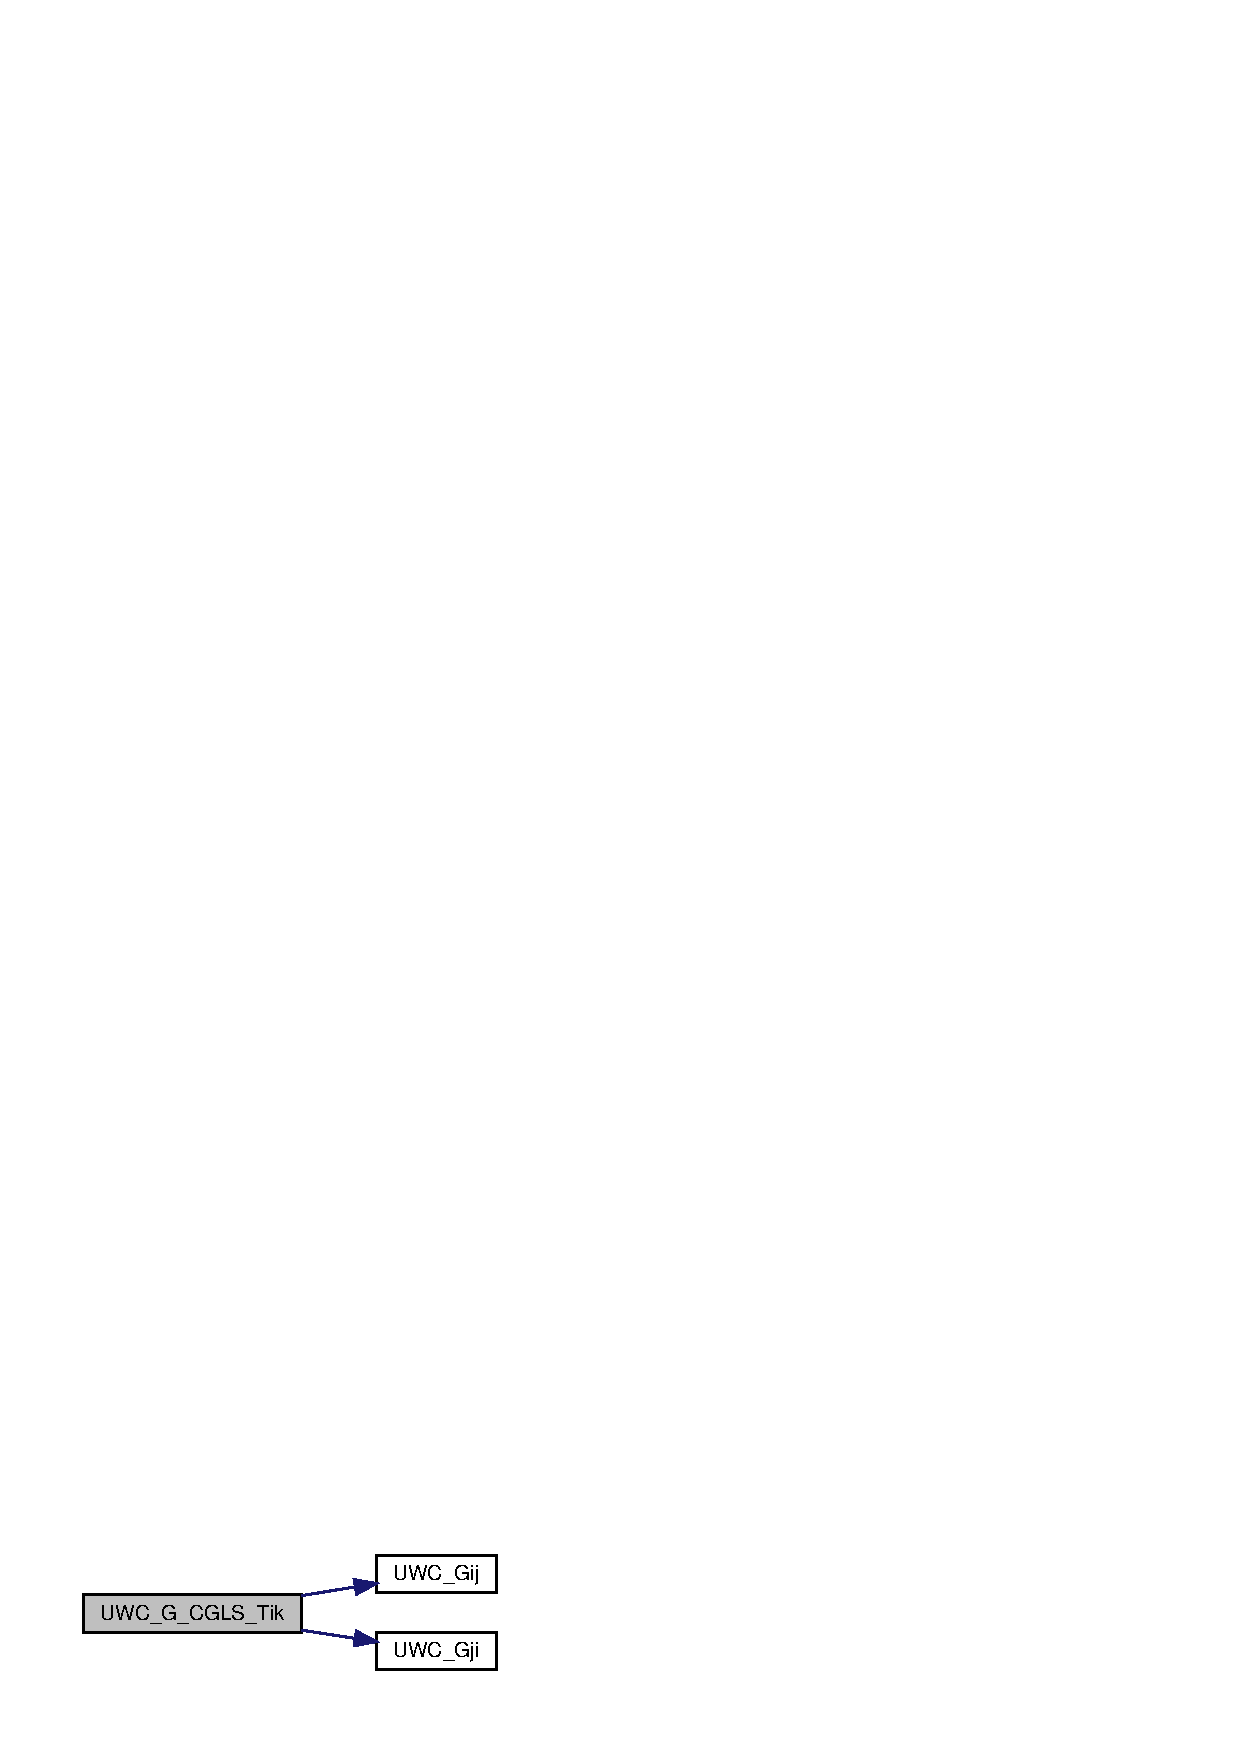
\includegraphics[width=242pt]{Conti2D_8cpp_a6e44071dbbec5b92ddf8673dea8c41de_a6e44071dbbec5b92ddf8673dea8c41de_cgraph}
\end{center}
\end{figure}
Here is the caller graph for this function\+:\nopagebreak
\begin{figure}[H]
\begin{center}
\leavevmode
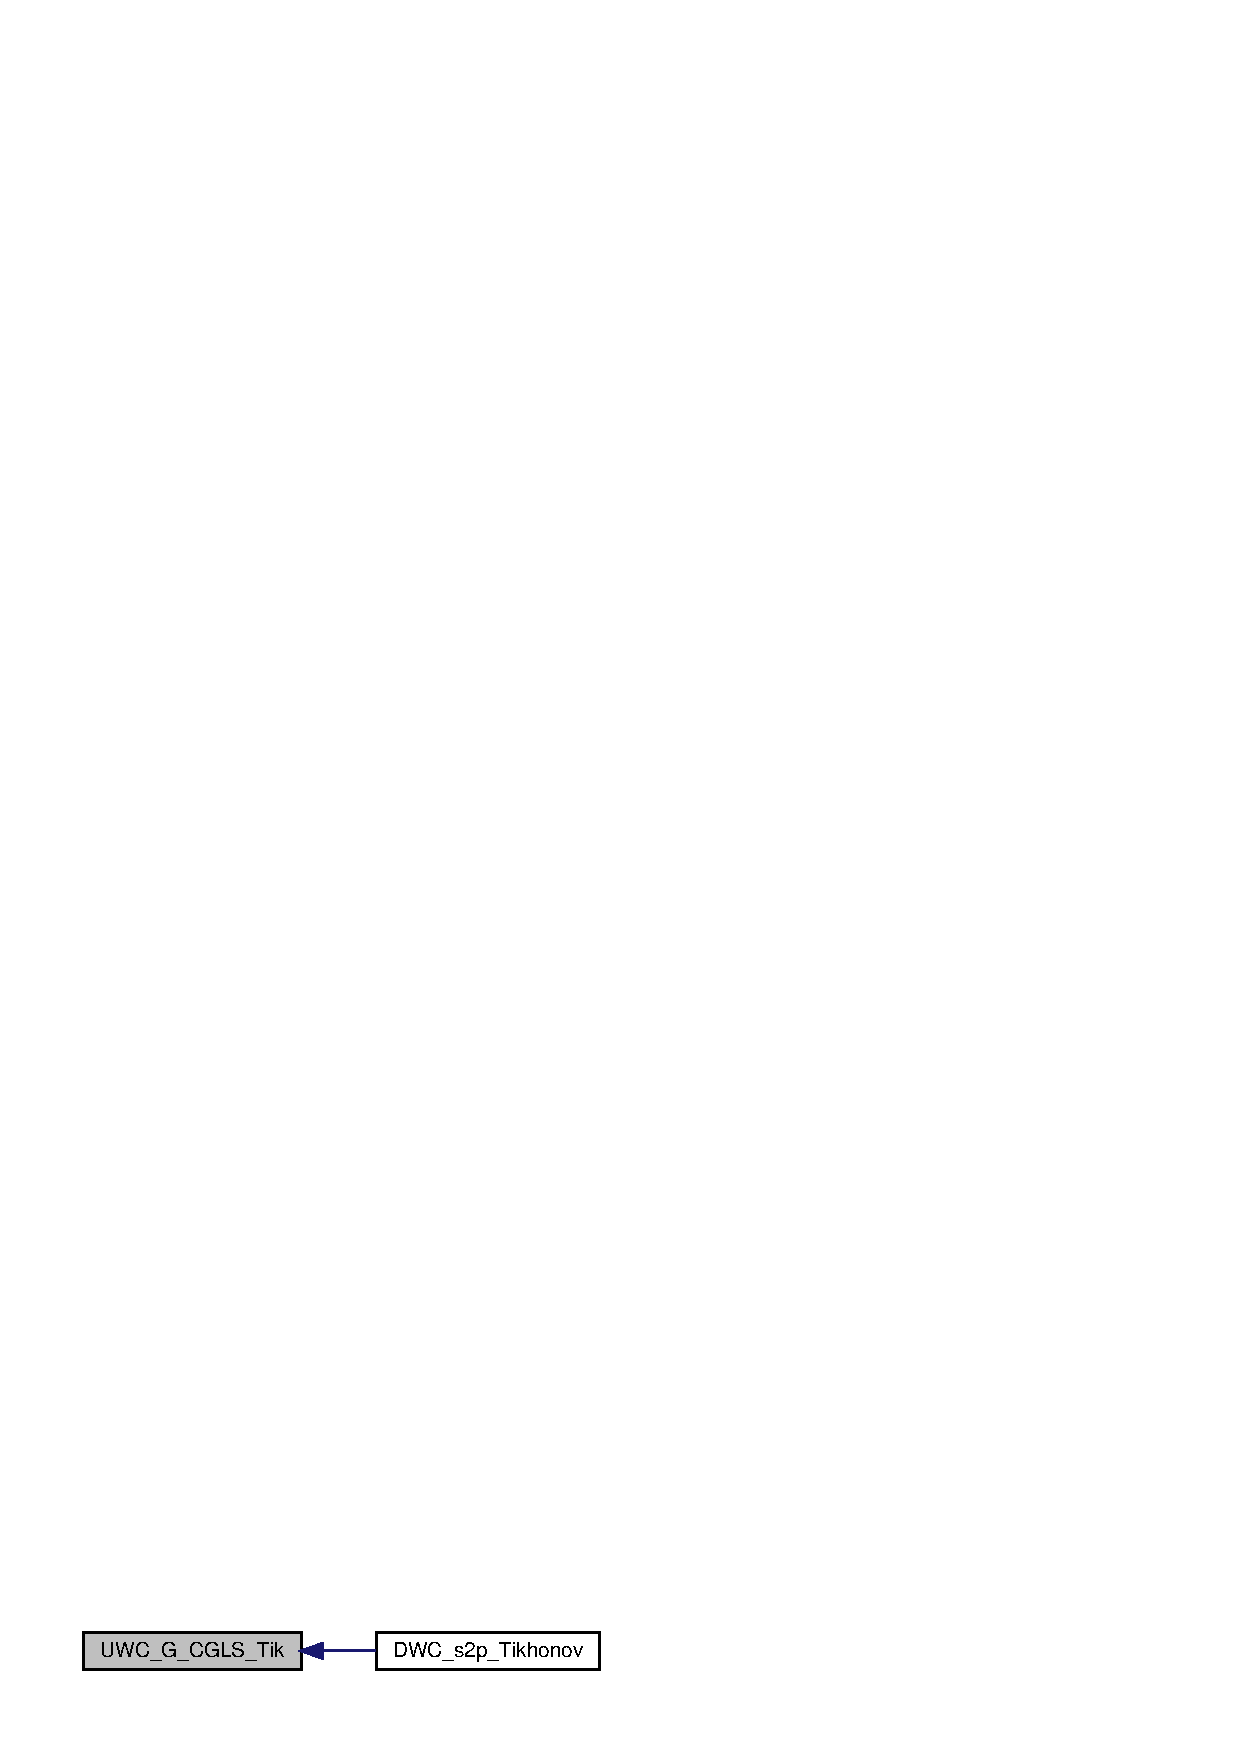
\includegraphics[width=292pt]{Conti2D_8cpp_a6e44071dbbec5b92ddf8673dea8c41de_a6e44071dbbec5b92ddf8673dea8c41de_icgraph}
\end{center}
\end{figure}
\mbox{\label{Conti2D_8cpp_a632c1e4efbb7e9b1aaf04db729e69394_a632c1e4efbb7e9b1aaf04db729e69394}} 
\index{Conti2\+D.\+cpp@{Conti2\+D.\+cpp}!U\+W\+C\+\_\+\+Gij@{U\+W\+C\+\_\+\+Gij}}
\index{U\+W\+C\+\_\+\+Gij@{U\+W\+C\+\_\+\+Gij}!Conti2\+D.\+cpp@{Conti2\+D.\+cpp}}
\subsubsection{U\+W\+C\+\_\+\+Gij()\hspace{0.1cm}{\footnotesize\ttfamily [1/2]}}
{\footnotesize\ttfamily void U\+W\+C\+\_\+\+Gij (\begin{DoxyParamCaption}\item[{double $\ast$}]{b,  }\item[{double $\ast$$\ast$}]{G,  }\item[{double $\ast$}]{x,  }\item[{int}]{modelnum,  }\item[{int}]{num\+\_\+thread }\end{DoxyParamCaption})}



Definition at line 900 of file Conti2\+D.\+cpp.



Referenced by D\+W\+C\+\_\+p2p\+\_\+\+C\+G\+L\+S(), D\+W\+C\+\_\+p2p\+\_\+\+Itegration\+Iter(), D\+W\+C\+\_\+p2p\+\_\+\+Landweber\+Iter(), D\+W\+C\+\_\+s2p\+\_\+\+C\+G\+L\+S(), D\+W\+C\+\_\+s2p\+\_\+\+Itegration\+Iter(), D\+W\+C\+\_\+s2p\+\_\+\+Landweber\+Iter(), D\+W\+C\+\_\+\+Tikhonov\+\_\+old(), U\+W\+C\+\_\+\+G\+\_\+\+C\+G\+L\+S\+\_\+\+Tik(), U\+W\+C\+\_\+p2p(), and U\+W\+C\+\_\+p2s().

Here is the caller graph for this function\+:\nopagebreak
\begin{figure}[H]
\begin{center}
\leavevmode
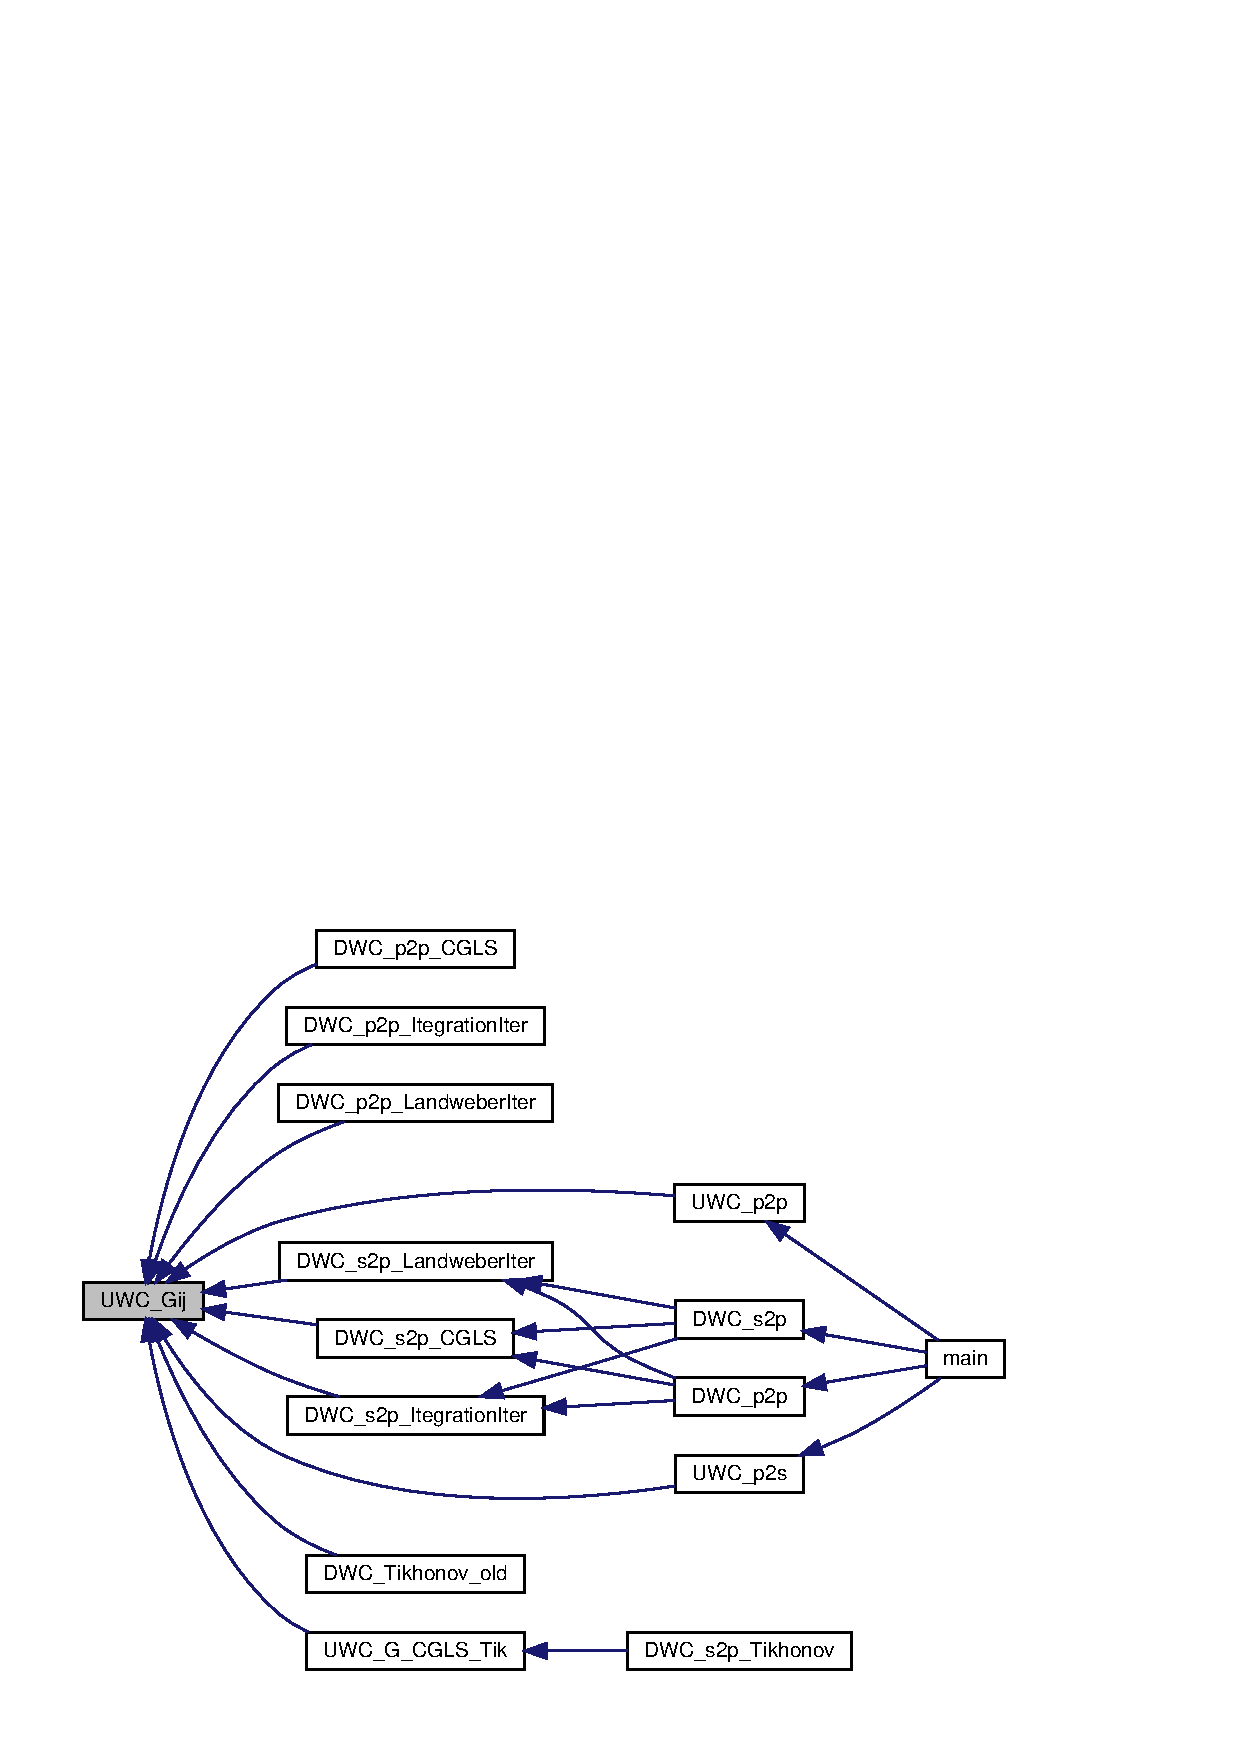
\includegraphics[width=350pt]{Conti2D_8cpp_a632c1e4efbb7e9b1aaf04db729e69394_a632c1e4efbb7e9b1aaf04db729e69394_icgraph}
\end{center}
\end{figure}
\mbox{\label{Conti2D_8cpp_a0cc3e78b4faaa9da0728fdc85057425d_a0cc3e78b4faaa9da0728fdc85057425d}} 
\index{Conti2\+D.\+cpp@{Conti2\+D.\+cpp}!U\+W\+C\+\_\+\+Gij@{U\+W\+C\+\_\+\+Gij}}
\index{U\+W\+C\+\_\+\+Gij@{U\+W\+C\+\_\+\+Gij}!Conti2\+D.\+cpp@{Conti2\+D.\+cpp}}
\subsubsection{U\+W\+C\+\_\+\+Gij()\hspace{0.1cm}{\footnotesize\ttfamily [2/2]}}
{\footnotesize\ttfamily void U\+W\+C\+\_\+\+Gij (\begin{DoxyParamCaption}\item[{double $\ast$}]{b,  }\item[{double $\ast$}]{G,  }\item[{double $\ast$}]{x,  }\item[{\textbf{ Grd\+Head}}]{grdhead,  }\item[{int}]{num\+\_\+thread }\end{DoxyParamCaption})}



Definition at line 938 of file Conti2\+D.\+cpp.



References Grd\+Head\+::cols, Get\+Gij(), and Grd\+Head\+::rows.

Here is the call graph for this function\+:
\nopagebreak
\begin{figure}[H]
\begin{center}
\leavevmode
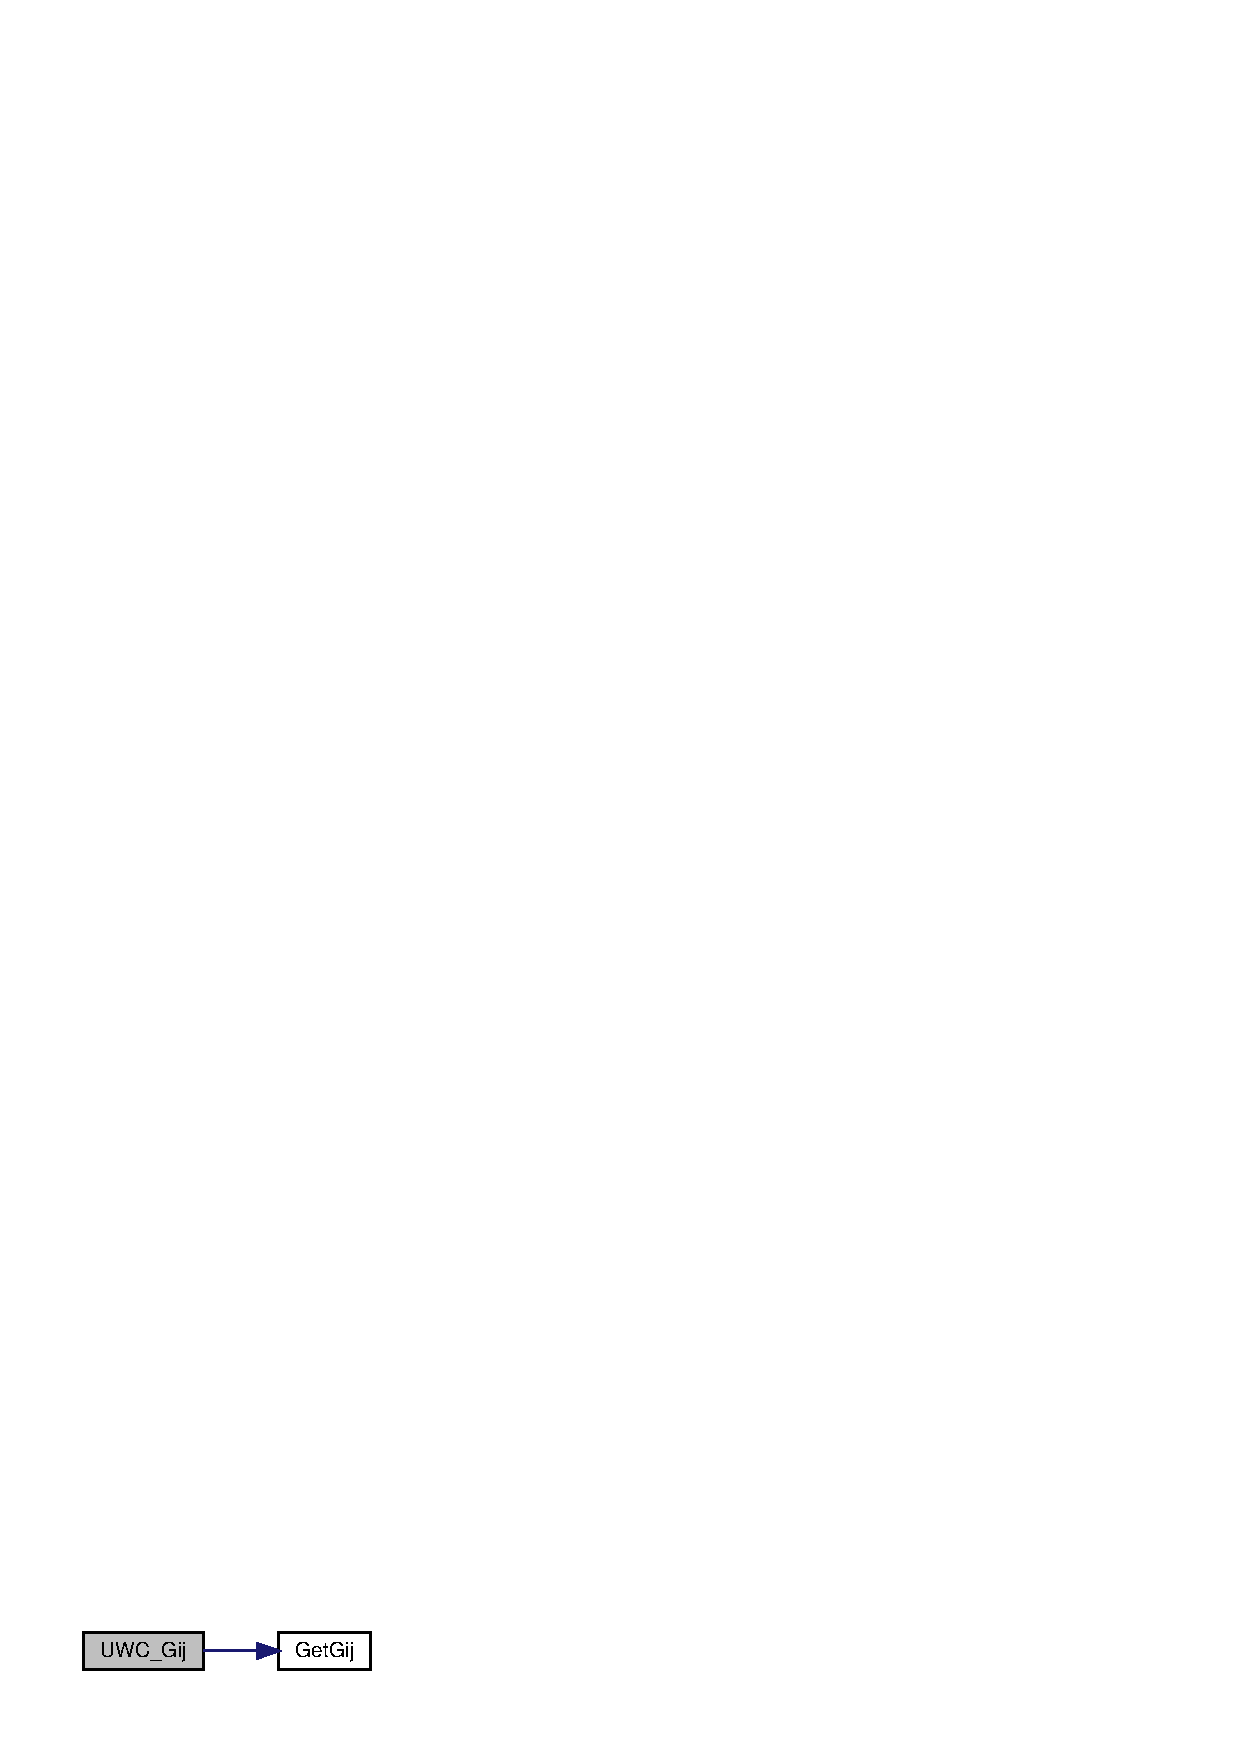
\includegraphics[width=182pt]{Conti2D_8cpp_a0cc3e78b4faaa9da0728fdc85057425d_a0cc3e78b4faaa9da0728fdc85057425d_cgraph}
\end{center}
\end{figure}
\mbox{\label{Conti2D_8cpp_a9d30373a0ff29e4f743eaf5e4cbc3cbf_a9d30373a0ff29e4f743eaf5e4cbc3cbf}} 
\index{Conti2\+D.\+cpp@{Conti2\+D.\+cpp}!U\+W\+C\+\_\+\+Gji@{U\+W\+C\+\_\+\+Gji}}
\index{U\+W\+C\+\_\+\+Gji@{U\+W\+C\+\_\+\+Gji}!Conti2\+D.\+cpp@{Conti2\+D.\+cpp}}
\subsubsection{U\+W\+C\+\_\+\+Gji()\hspace{0.1cm}{\footnotesize\ttfamily [1/2]}}
{\footnotesize\ttfamily void U\+W\+C\+\_\+\+Gji (\begin{DoxyParamCaption}\item[{double $\ast$}]{b,  }\item[{double $\ast$$\ast$}]{G,  }\item[{double $\ast$}]{x,  }\item[{int}]{modelnum,  }\item[{int}]{num\+\_\+thread }\end{DoxyParamCaption})}



Definition at line 879 of file Conti2\+D.\+cpp.



Referenced by D\+W\+C\+\_\+p2p\+\_\+\+C\+G\+L\+S(), D\+W\+C\+\_\+s2p\+\_\+\+C\+G\+L\+S(), D\+W\+C\+\_\+s2p\+\_\+\+Tikhonov(), and U\+W\+C\+\_\+\+G\+\_\+\+C\+G\+L\+S\+\_\+\+Tik().

Here is the caller graph for this function\+:\nopagebreak
\begin{figure}[H]
\begin{center}
\leavevmode
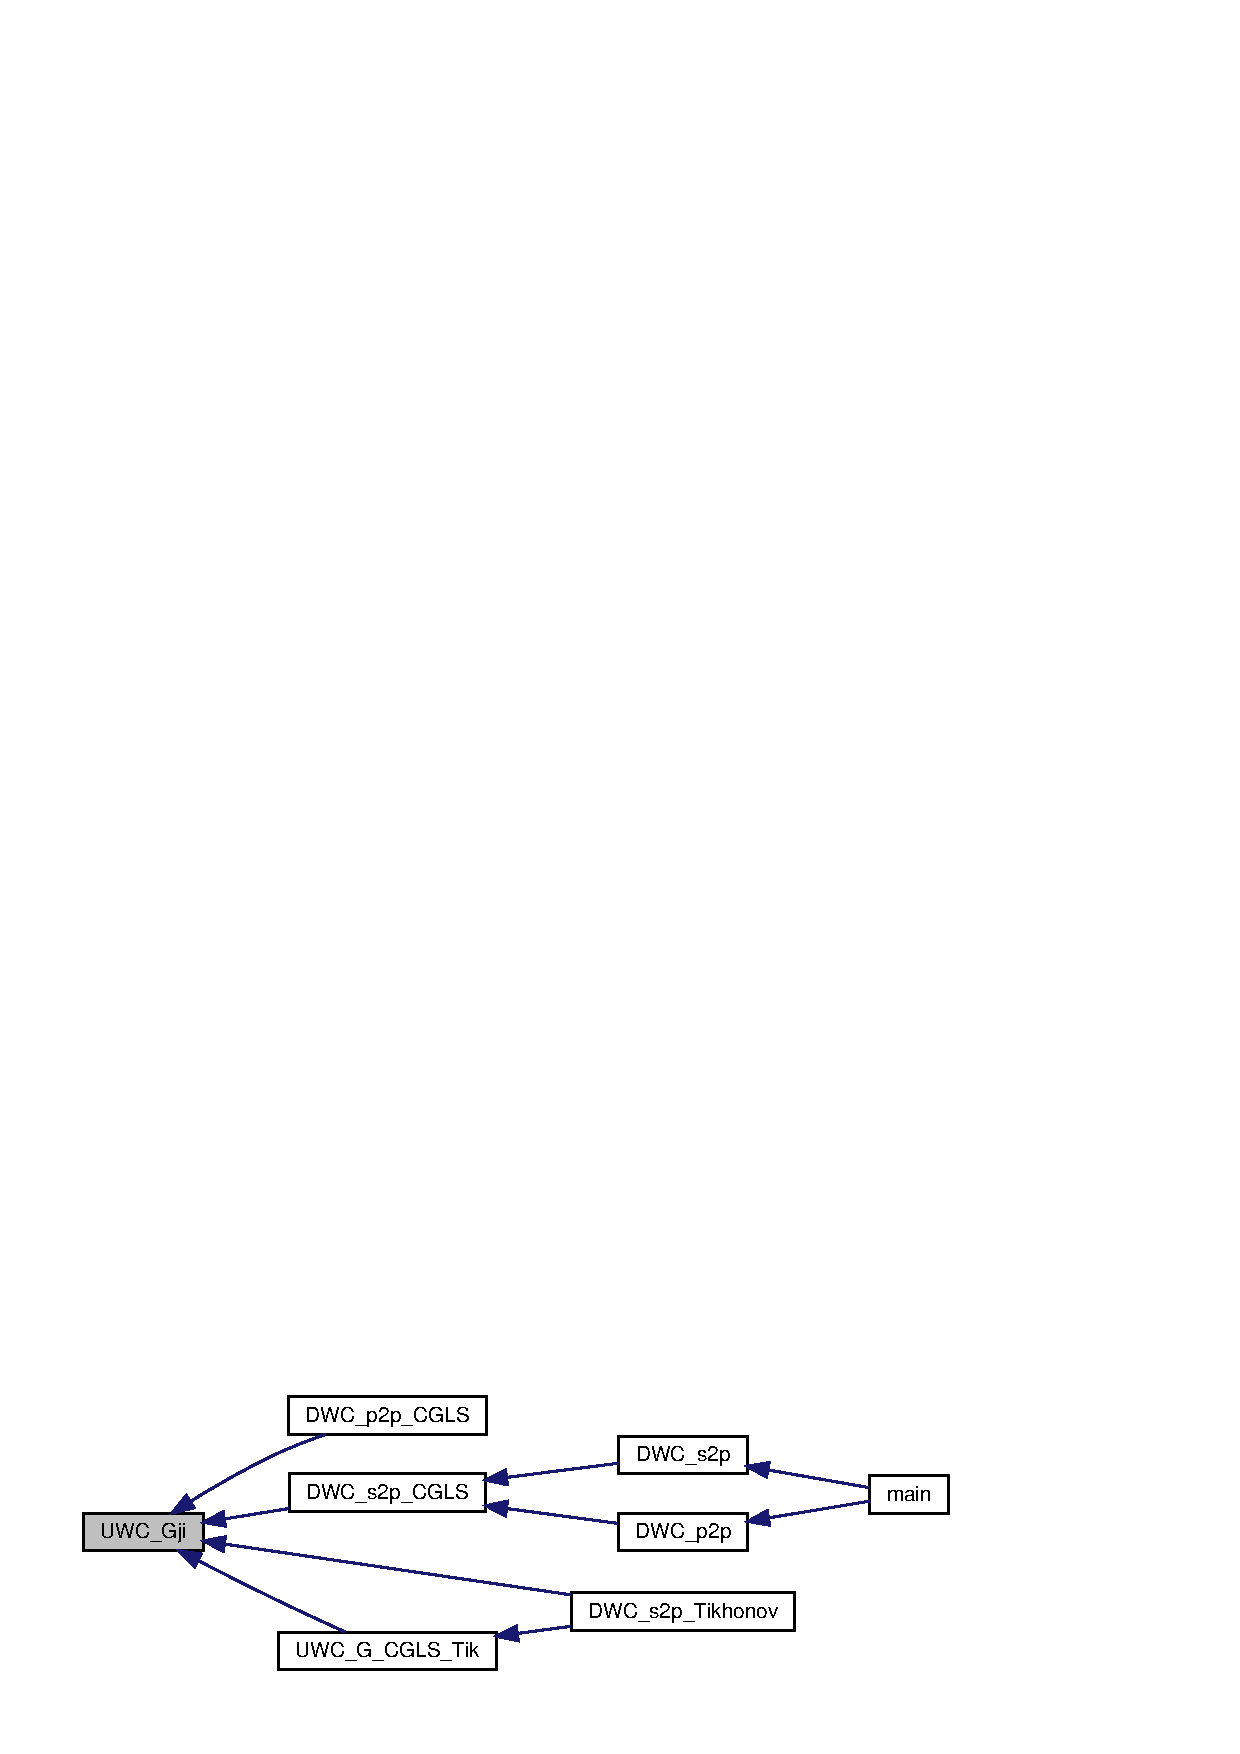
\includegraphics[width=350pt]{Conti2D_8cpp_a9d30373a0ff29e4f743eaf5e4cbc3cbf_a9d30373a0ff29e4f743eaf5e4cbc3cbf_icgraph}
\end{center}
\end{figure}
\mbox{\label{Conti2D_8cpp_a7ab8990653bc3bdbef25f3b17e949f0f_a7ab8990653bc3bdbef25f3b17e949f0f}} 
\index{Conti2\+D.\+cpp@{Conti2\+D.\+cpp}!U\+W\+C\+\_\+\+Gji@{U\+W\+C\+\_\+\+Gji}}
\index{U\+W\+C\+\_\+\+Gji@{U\+W\+C\+\_\+\+Gji}!Conti2\+D.\+cpp@{Conti2\+D.\+cpp}}
\subsubsection{U\+W\+C\+\_\+\+Gji()\hspace{0.1cm}{\footnotesize\ttfamily [2/2]}}
{\footnotesize\ttfamily void U\+W\+C\+\_\+\+Gji (\begin{DoxyParamCaption}\item[{double $\ast$}]{b,  }\item[{double $\ast$}]{G,  }\item[{double $\ast$}]{x,  }\item[{\textbf{ Grd\+Head}}]{grdhead,  }\item[{int}]{num\+\_\+thread }\end{DoxyParamCaption})}



Definition at line 921 of file Conti2\+D.\+cpp.



References Grd\+Head\+::cols, Get\+Gij(), and Grd\+Head\+::rows.

Here is the call graph for this function\+:
\nopagebreak
\begin{figure}[H]
\begin{center}
\leavevmode
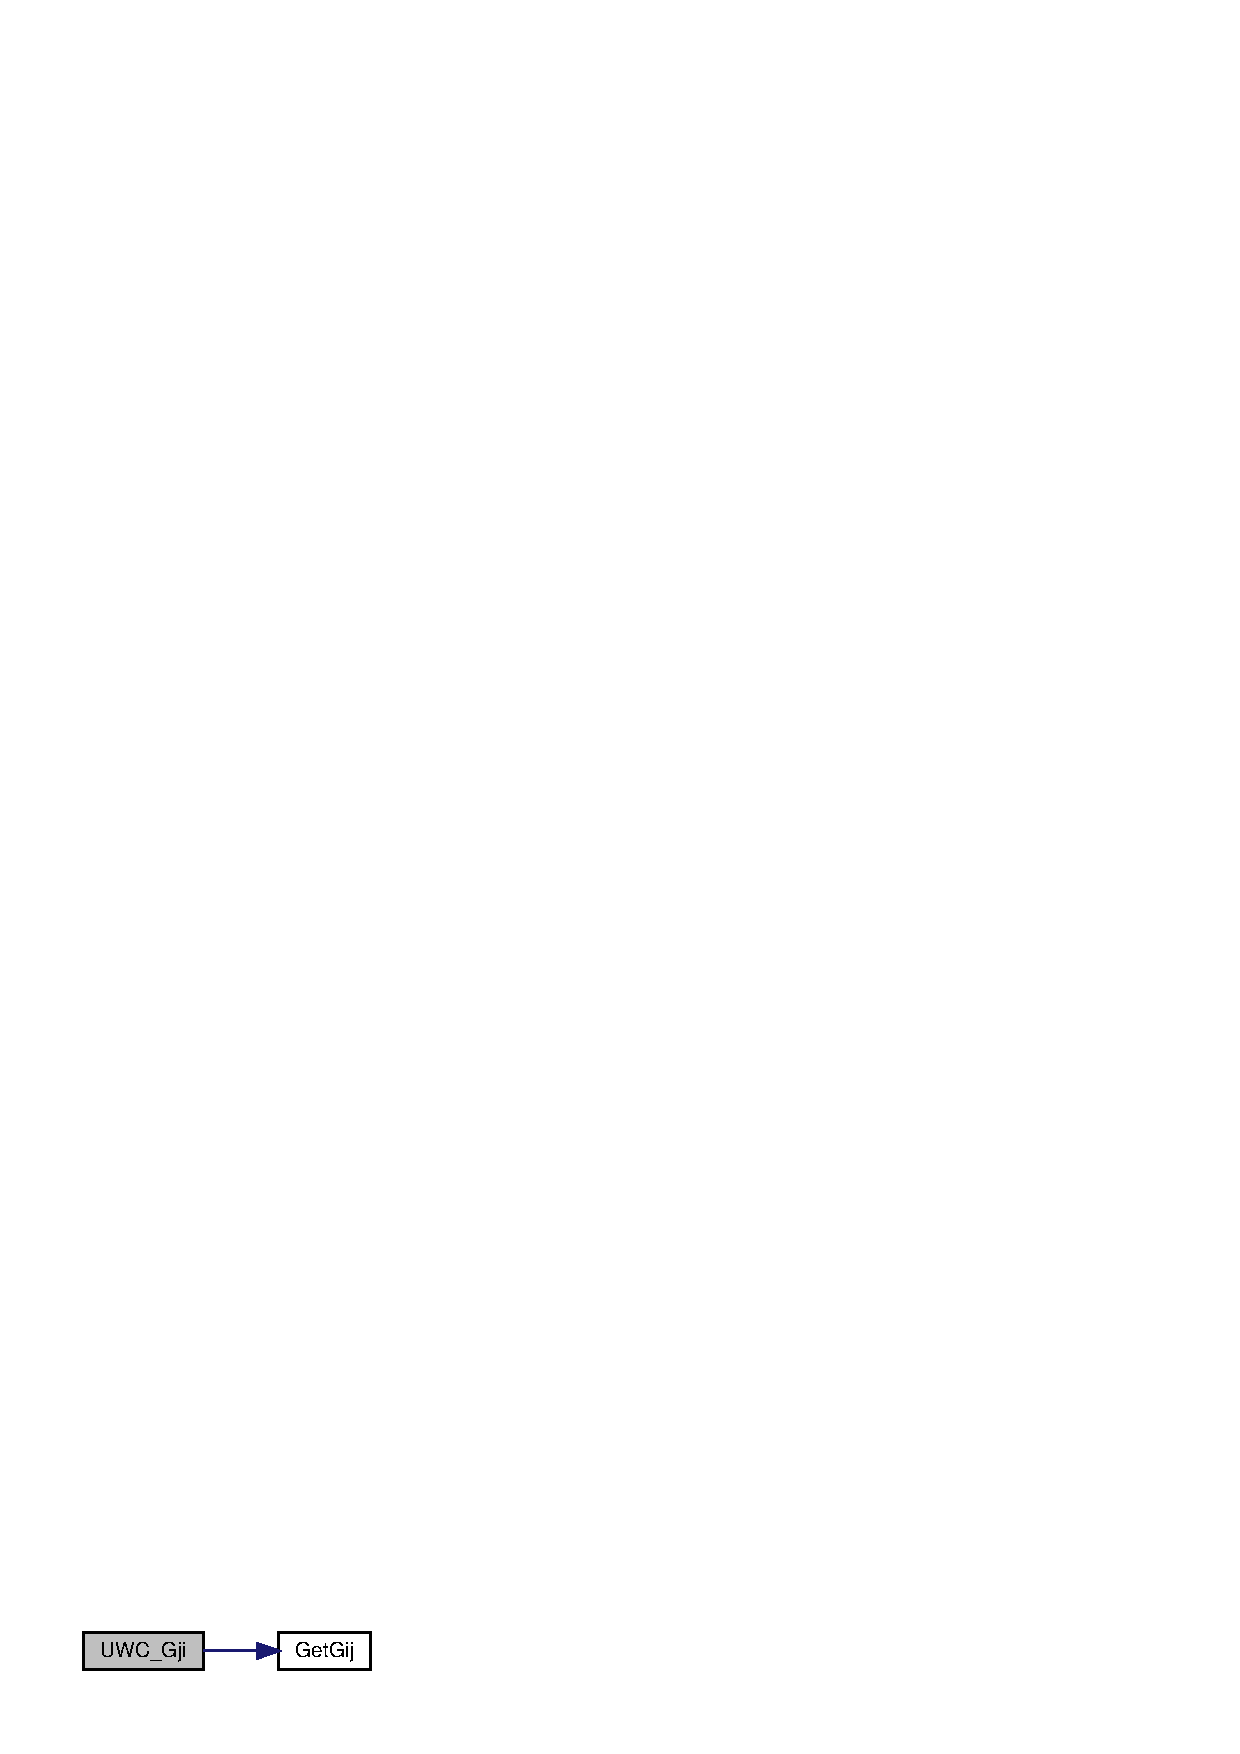
\includegraphics[width=182pt]{Conti2D_8cpp_a7ab8990653bc3bdbef25f3b17e949f0f_a7ab8990653bc3bdbef25f3b17e949f0f_cgraph}
\end{center}
\end{figure}
\mbox{\label{Conti2D_8cpp_a7b6bfe9f5b32bc1a62005196d84edfde_a7b6bfe9f5b32bc1a62005196d84edfde}} 
\index{Conti2\+D.\+cpp@{Conti2\+D.\+cpp}!U\+W\+C\+\_\+p2p@{U\+W\+C\+\_\+p2p}}
\index{U\+W\+C\+\_\+p2p@{U\+W\+C\+\_\+p2p}!Conti2\+D.\+cpp@{Conti2\+D.\+cpp}}
\subsubsection{U\+W\+C\+\_\+p2p()}
{\footnotesize\ttfamily void U\+W\+C\+\_\+p2p (\begin{DoxyParamCaption}\item[{string}]{inputfilename,  }\item[{string}]{outputfilename,  }\item[{double}]{height1,  }\item[{double}]{height2,  }\item[{int}]{ext\+Num,  }\item[{int}]{num\+\_\+thread,  }\item[{bool}]{is\+Progress,  }\item[{bool}]{use\+Old\+Kernel,  }\item[{string}]{filename\+\_\+exact }\end{DoxyParamCaption})}



Definition at line 400 of file Conti2\+D.\+cpp.



References Grd\+Head\+::cols, Getkernel\+\_\+p2p\+\_\+new(), Read\+Grd(), Grd\+Head\+::rows, Save\+Grd(), and U\+W\+C\+\_\+\+Gij().



Referenced by main().

Here is the call graph for this function\+:
\nopagebreak
\begin{figure}[H]
\begin{center}
\leavevmode
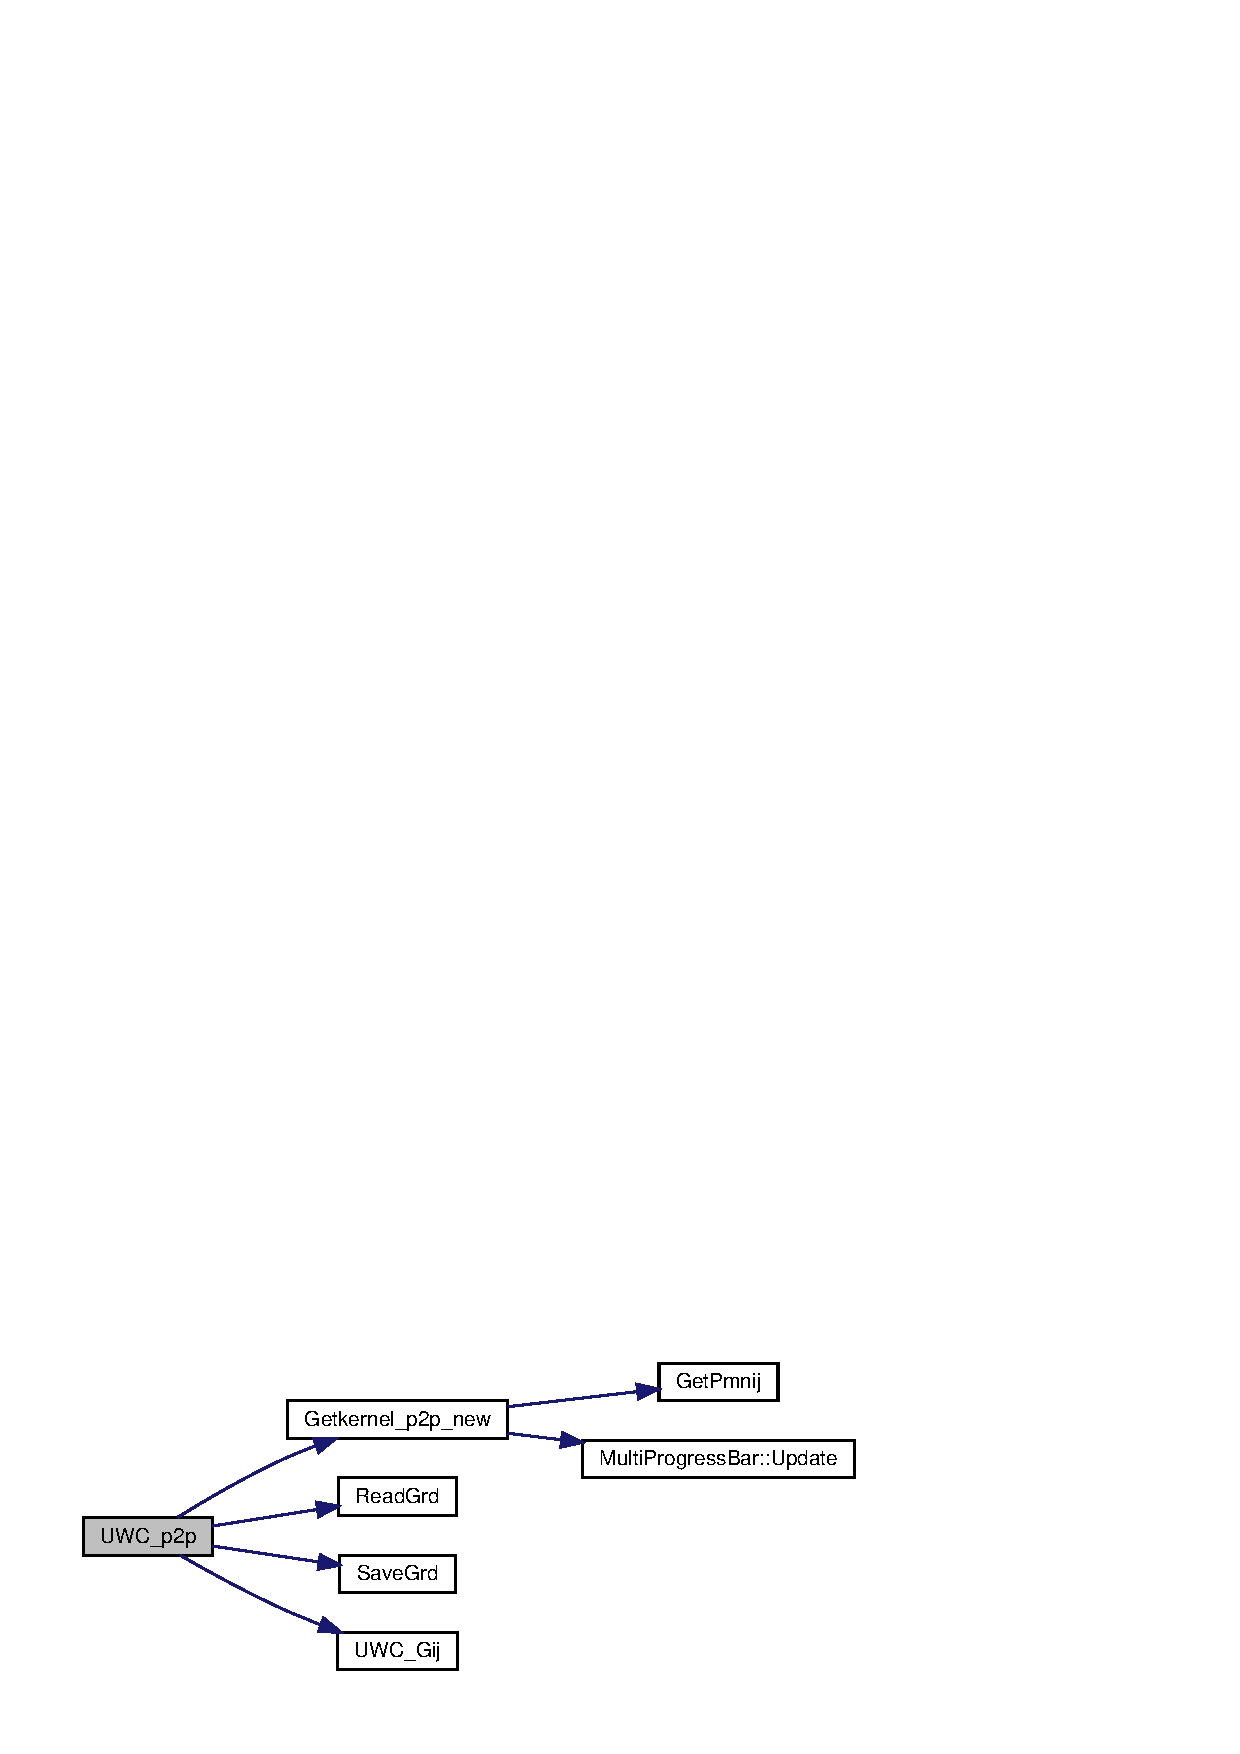
\includegraphics[width=350pt]{Conti2D_8cpp_a7b6bfe9f5b32bc1a62005196d84edfde_a7b6bfe9f5b32bc1a62005196d84edfde_cgraph}
\end{center}
\end{figure}
Here is the caller graph for this function\+:\nopagebreak
\begin{figure}[H]
\begin{center}
\leavevmode
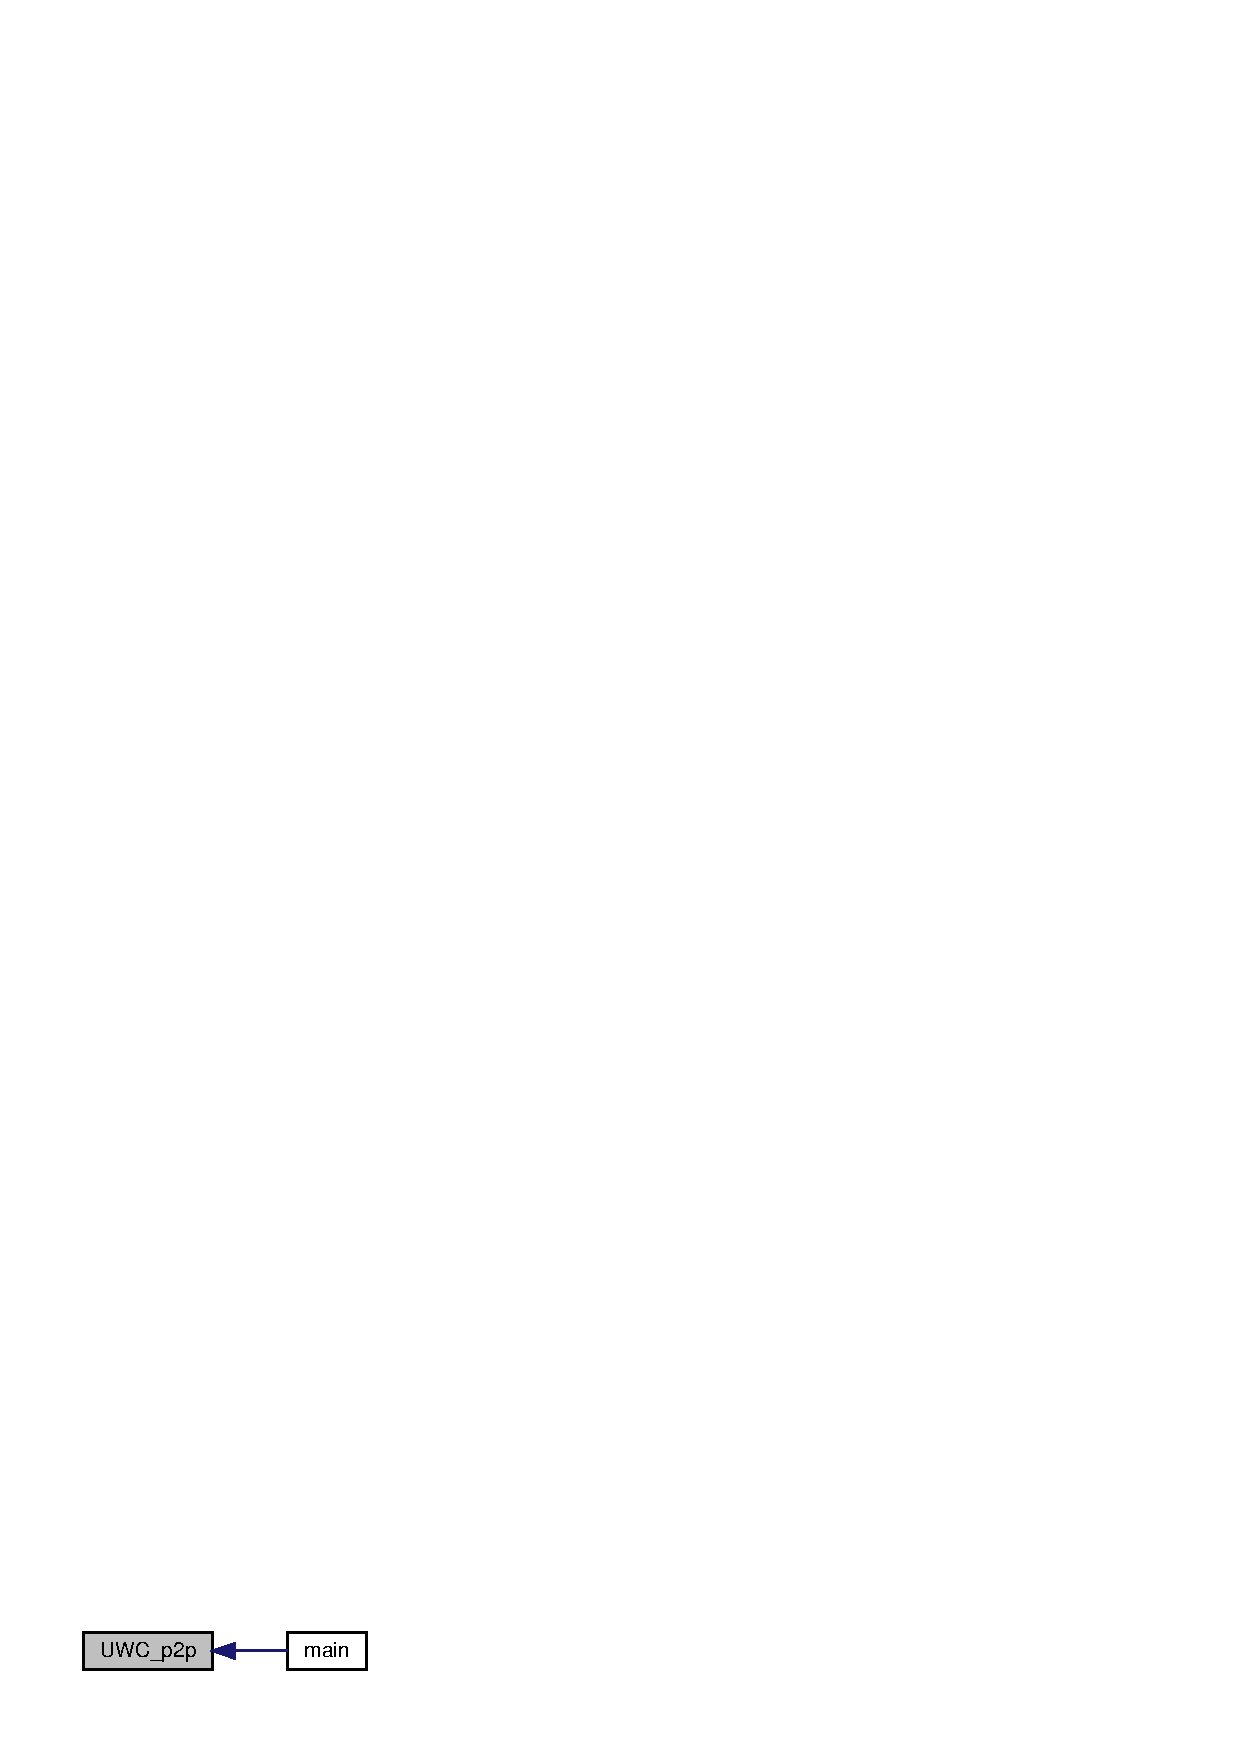
\includegraphics[width=180pt]{Conti2D_8cpp_a7b6bfe9f5b32bc1a62005196d84edfde_a7b6bfe9f5b32bc1a62005196d84edfde_icgraph}
\end{center}
\end{figure}
\mbox{\label{Conti2D_8cpp_af82757cb7e0f4f398e774b4e89b9ea72_af82757cb7e0f4f398e774b4e89b9ea72}} 
\index{Conti2\+D.\+cpp@{Conti2\+D.\+cpp}!U\+W\+C\+\_\+p2p\+\_\+f@{U\+W\+C\+\_\+p2p\+\_\+f}}
\index{U\+W\+C\+\_\+p2p\+\_\+f@{U\+W\+C\+\_\+p2p\+\_\+f}!Conti2\+D.\+cpp@{Conti2\+D.\+cpp}}
\subsubsection{U\+W\+C\+\_\+p2p\+\_\+f()\hspace{0.1cm}{\footnotesize\ttfamily [1/2]}}
{\footnotesize\ttfamily void U\+W\+C\+\_\+p2p\+\_\+f (\begin{DoxyParamCaption}\item[{string}]{inputfilename,  }\item[{string}]{outputfilename,  }\item[{double}]{height1,  }\item[{double}]{height2,  }\item[{int}]{ext\+Num,  }\item[{string}]{filename\+\_\+exact }\end{DoxyParamCaption})}



Definition at line 479 of file Conti2\+D.\+cpp.



References Grd\+Head\+::cols, Read\+Grd(), Grd\+Head\+::rows, Save\+Grd(), and U\+W\+C\+\_\+p2p\+\_\+f().



Referenced by D\+W\+C\+\_\+p2p\+\_\+f(), main(), and U\+W\+C\+\_\+p2p\+\_\+f().

Here is the call graph for this function\+:
\nopagebreak
\begin{figure}[H]
\begin{center}
\leavevmode
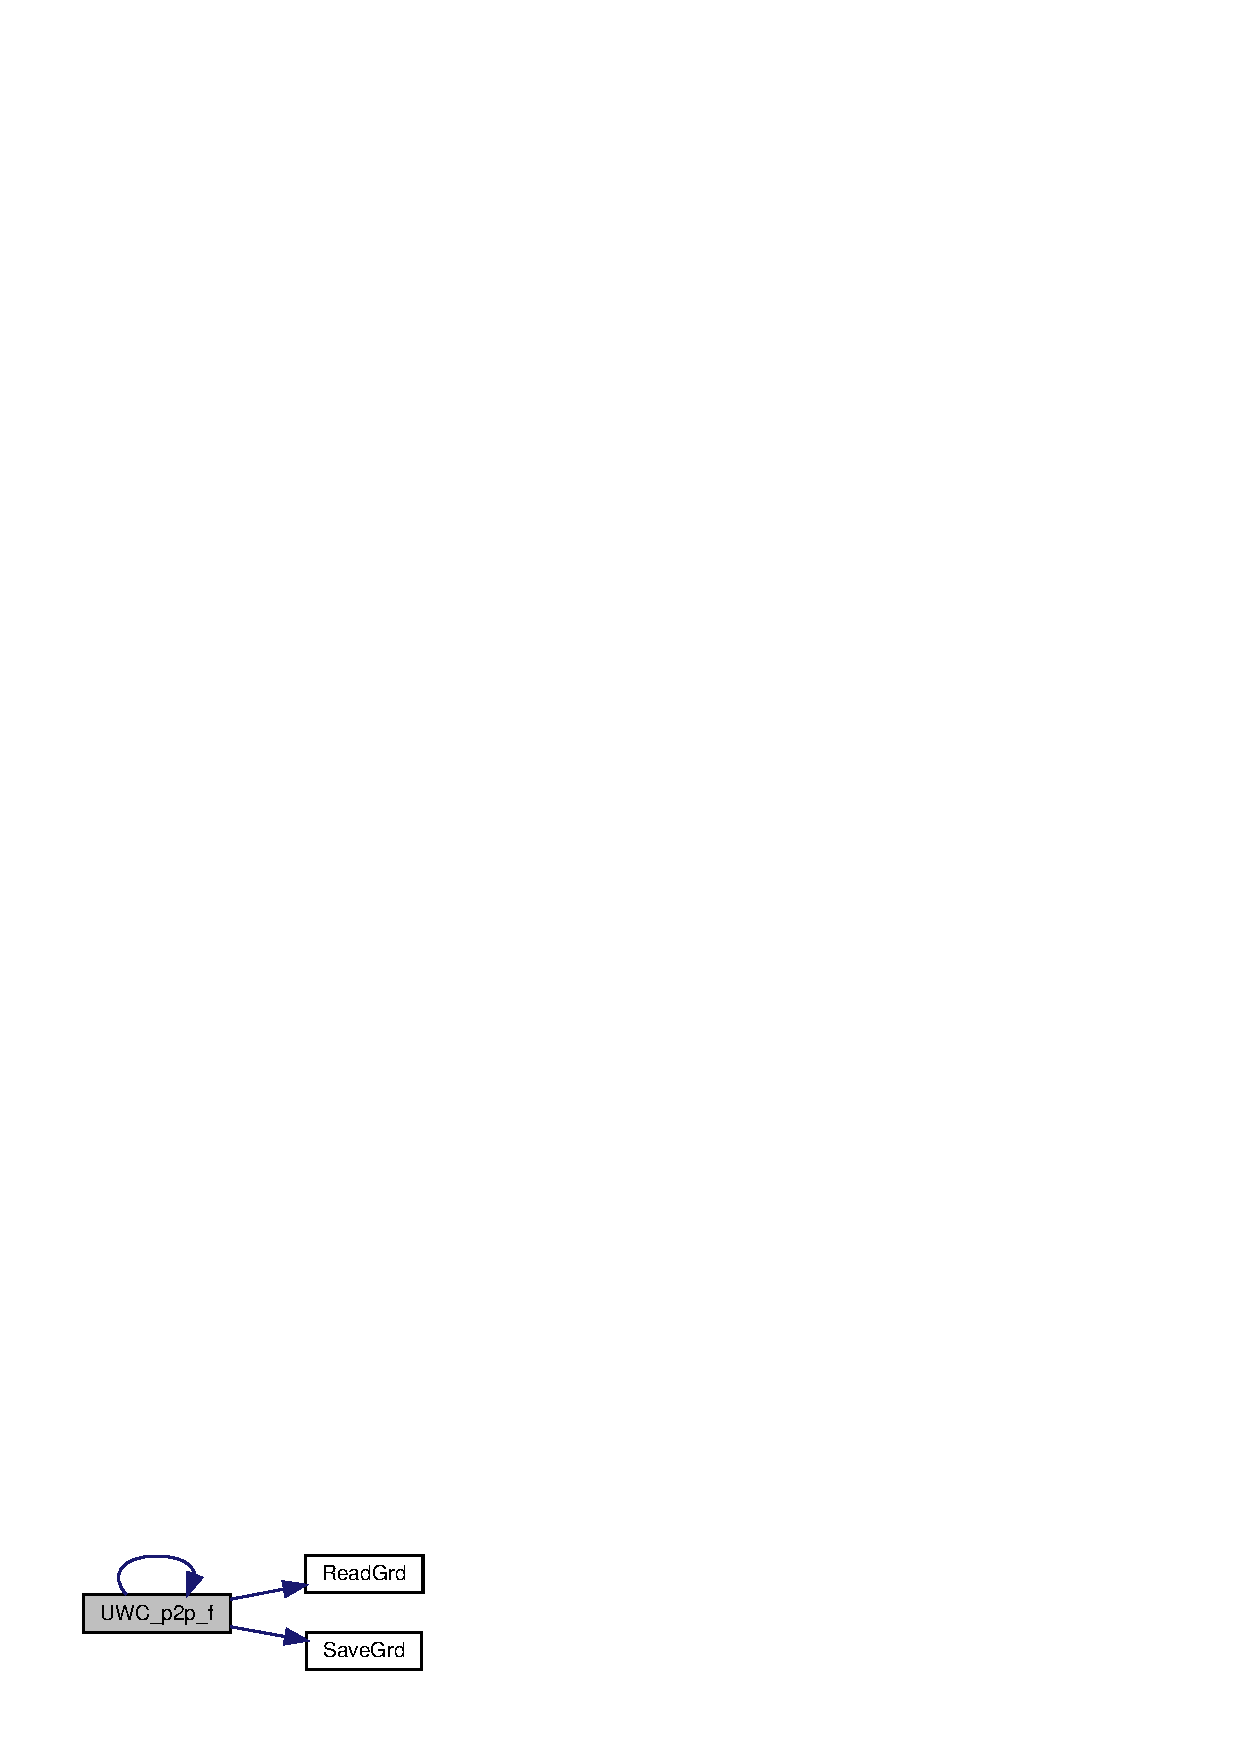
\includegraphics[width=207pt]{Conti2D_8cpp_af82757cb7e0f4f398e774b4e89b9ea72_af82757cb7e0f4f398e774b4e89b9ea72_cgraph}
\end{center}
\end{figure}
Here is the caller graph for this function\+:\nopagebreak
\begin{figure}[H]
\begin{center}
\leavevmode
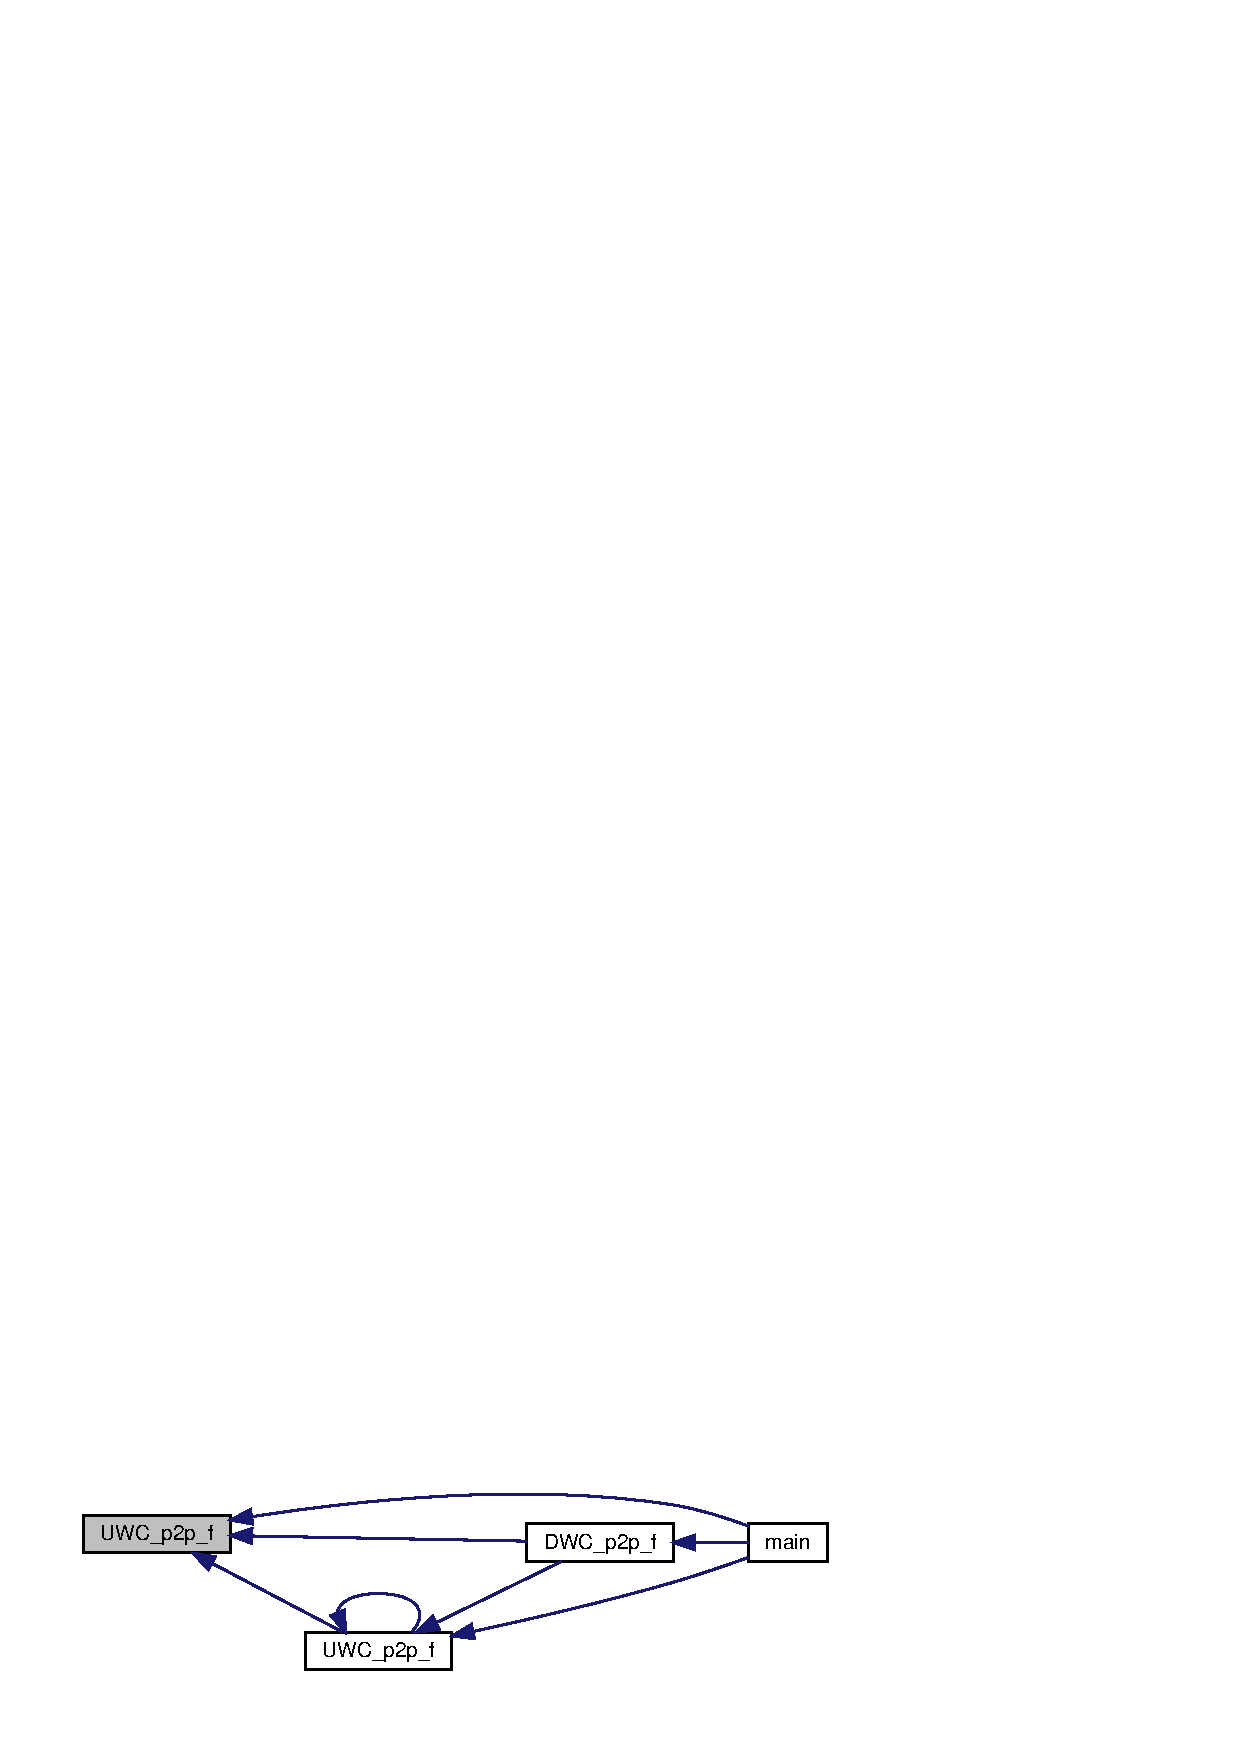
\includegraphics[width=350pt]{Conti2D_8cpp_af82757cb7e0f4f398e774b4e89b9ea72_af82757cb7e0f4f398e774b4e89b9ea72_icgraph}
\end{center}
\end{figure}
\mbox{\label{Conti2D_8cpp_a016dc620865e33635aabc81c129eac30_a016dc620865e33635aabc81c129eac30}} 
\index{Conti2\+D.\+cpp@{Conti2\+D.\+cpp}!U\+W\+C\+\_\+p2p\+\_\+f@{U\+W\+C\+\_\+p2p\+\_\+f}}
\index{U\+W\+C\+\_\+p2p\+\_\+f@{U\+W\+C\+\_\+p2p\+\_\+f}!Conti2\+D.\+cpp@{Conti2\+D.\+cpp}}
\subsubsection{U\+W\+C\+\_\+p2p\+\_\+f()\hspace{0.1cm}{\footnotesize\ttfamily [2/2]}}
{\footnotesize\ttfamily int U\+W\+C\+\_\+p2p\+\_\+f (\begin{DoxyParamCaption}\item[{double $\ast$}]{inputdata,  }\item[{double $\ast$}]{result,  }\item[{\textbf{ Grd\+Head}}]{grdhead,  }\item[{double}]{rph }\end{DoxyParamCaption})}



Definition at line 517 of file Conti2\+D.\+cpp.



References Grd\+Head\+::bounds, Grd\+Head\+::cols, F\+F\+T2d(), I\+F\+F\+T2d(), PI, and Grd\+Head\+::rows.

Here is the call graph for this function\+:\nopagebreak
\begin{figure}[H]
\begin{center}
\leavevmode
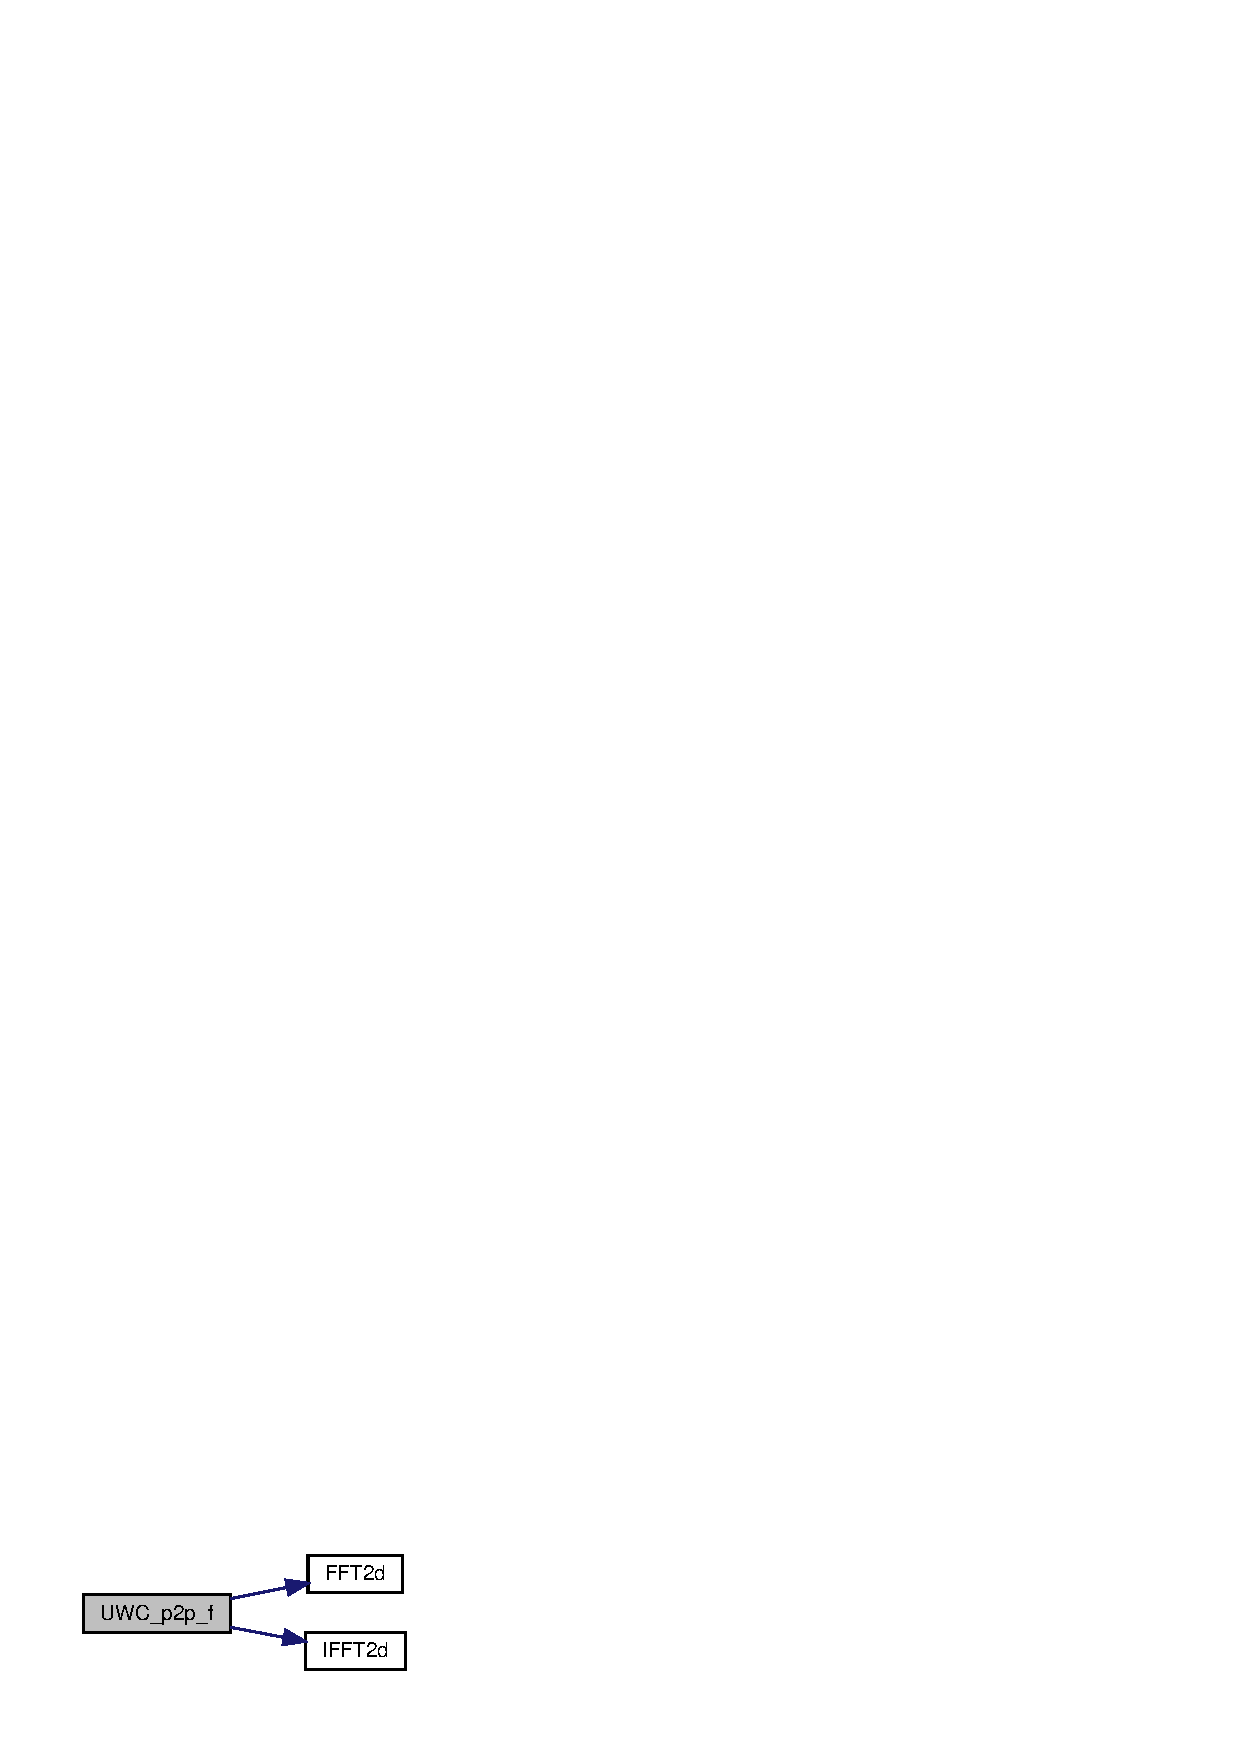
\includegraphics[width=199pt]{Conti2D_8cpp_a016dc620865e33635aabc81c129eac30_a016dc620865e33635aabc81c129eac30_cgraph}
\end{center}
\end{figure}
\mbox{\label{Conti2D_8cpp_af8adb87017663774bfd342b39facc828_af8adb87017663774bfd342b39facc828}} 
\index{Conti2\+D.\+cpp@{Conti2\+D.\+cpp}!U\+W\+C\+\_\+p2s@{U\+W\+C\+\_\+p2s}}
\index{U\+W\+C\+\_\+p2s@{U\+W\+C\+\_\+p2s}!Conti2\+D.\+cpp@{Conti2\+D.\+cpp}}
\subsubsection{U\+W\+C\+\_\+p2s()}
{\footnotesize\ttfamily void U\+W\+C\+\_\+p2s (\begin{DoxyParamCaption}\item[{string}]{inputfilename,  }\item[{string}]{outputfilename,  }\item[{double}]{height1,  }\item[{string}]{topo\+File,  }\item[{int}]{ext\+Num,  }\item[{int}]{num\+\_\+thread,  }\item[{bool}]{is\+Progress,  }\item[{bool}]{use\+Old\+Kernel,  }\item[{string}]{filename\+\_\+exact }\end{DoxyParamCaption})}



Definition at line 320 of file Conti2\+D.\+cpp.



References C\+O\+L\+O\+R\+\_\+\+D\+E\+F\+A\+L\+UT, Grd\+Head\+::cols, Getkernel\+\_\+p2s\+\_\+new(), Read\+Grd(), R\+ED, Grd\+Head\+::rows, Save\+Grd(), and U\+W\+C\+\_\+\+Gij().



Referenced by main().

Here is the call graph for this function\+:
\nopagebreak
\begin{figure}[H]
\begin{center}
\leavevmode
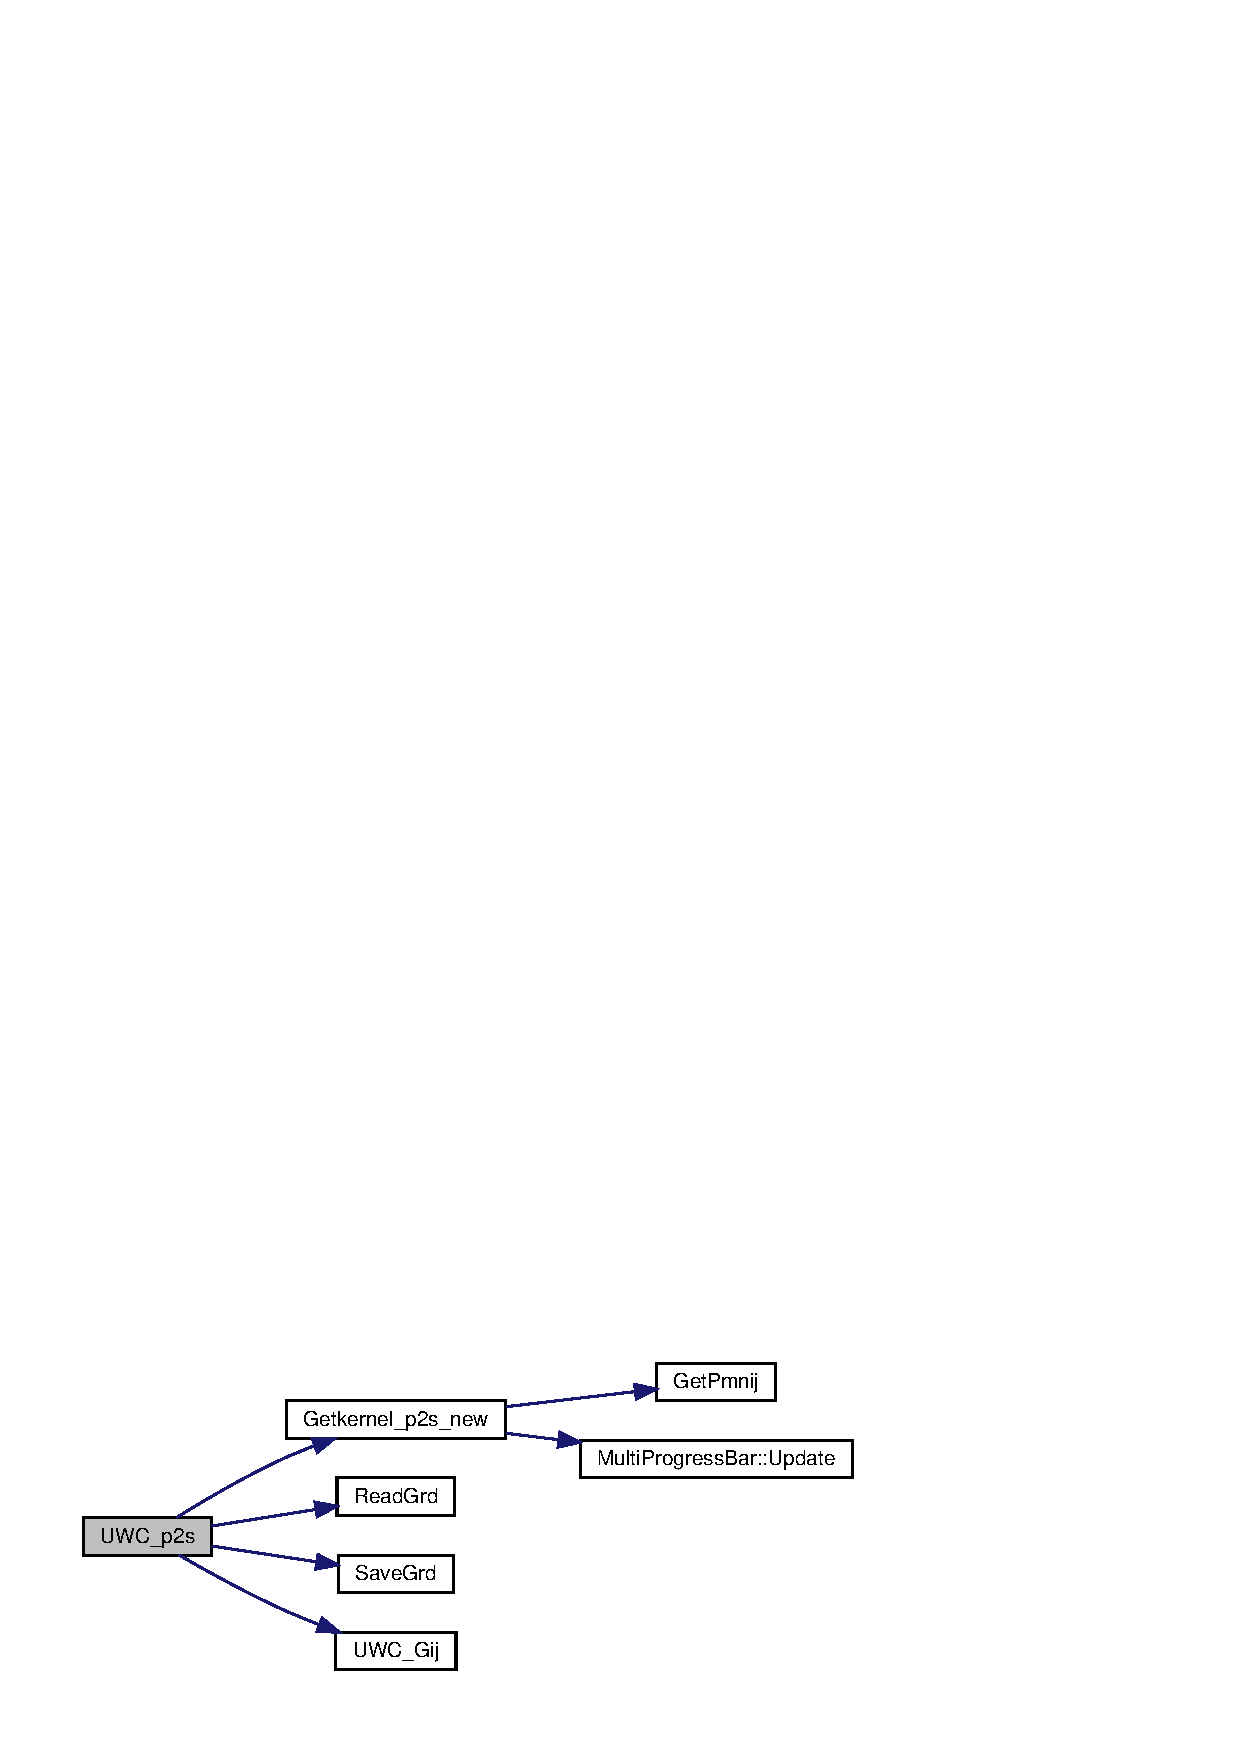
\includegraphics[width=350pt]{Conti2D_8cpp_af8adb87017663774bfd342b39facc828_af8adb87017663774bfd342b39facc828_cgraph}
\end{center}
\end{figure}
Here is the caller graph for this function\+:\nopagebreak
\begin{figure}[H]
\begin{center}
\leavevmode
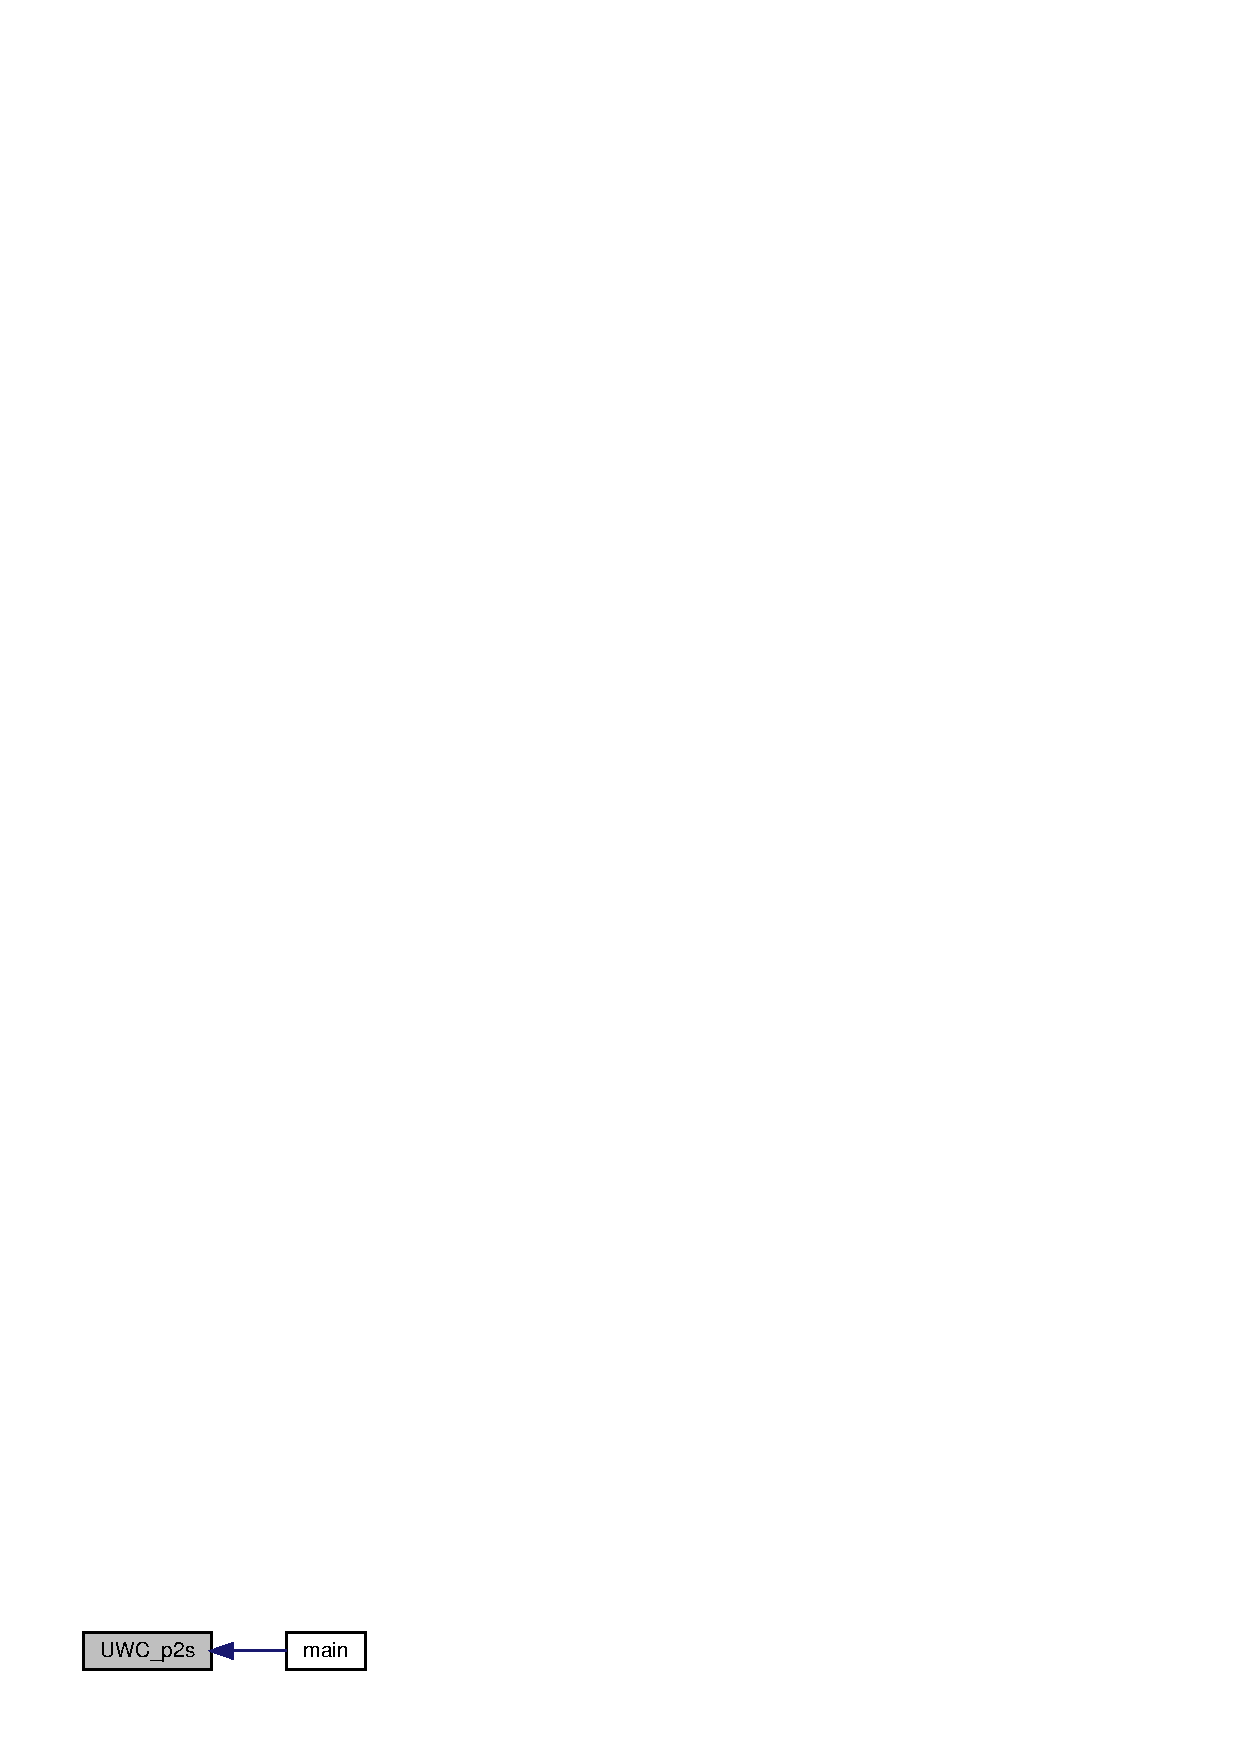
\includegraphics[width=179pt]{Conti2D_8cpp_af8adb87017663774bfd342b39facc828_af8adb87017663774bfd342b39facc828_icgraph}
\end{center}
\end{figure}

\section{Conti2\+D.\+h File Reference}
\label{Conti2D_8h}\index{Conti2\+D.\+h@{Conti2\+D.\+h}}
{\ttfamily \#include $<$sstream$>$}\newline
{\ttfamily \#include $<$iostream$>$}\newline
{\ttfamily \#include $<$fstream$>$}\newline
{\ttfamily \#include $<$iomanip$>$}\newline
{\ttfamily \#include $<$vector$>$}\newline
{\ttfamily \#include $<$math.\+h$>$}\newline
{\ttfamily \#include \char`\"{}omp.\+h\char`\"{}}\newline
{\ttfamily \#include \char`\"{}F\+F\+T\+N.\+h\char`\"{}}\newline
{\ttfamily \#include \char`\"{}Multi\+Progress\+Bar.\+h\char`\"{}}\newline
{\ttfamily \#include $<$unistd.\+h$>$}\newline
Include dependency graph for Conti2\+D.\+h\+:\nopagebreak
\begin{figure}[H]
\begin{center}
\leavevmode
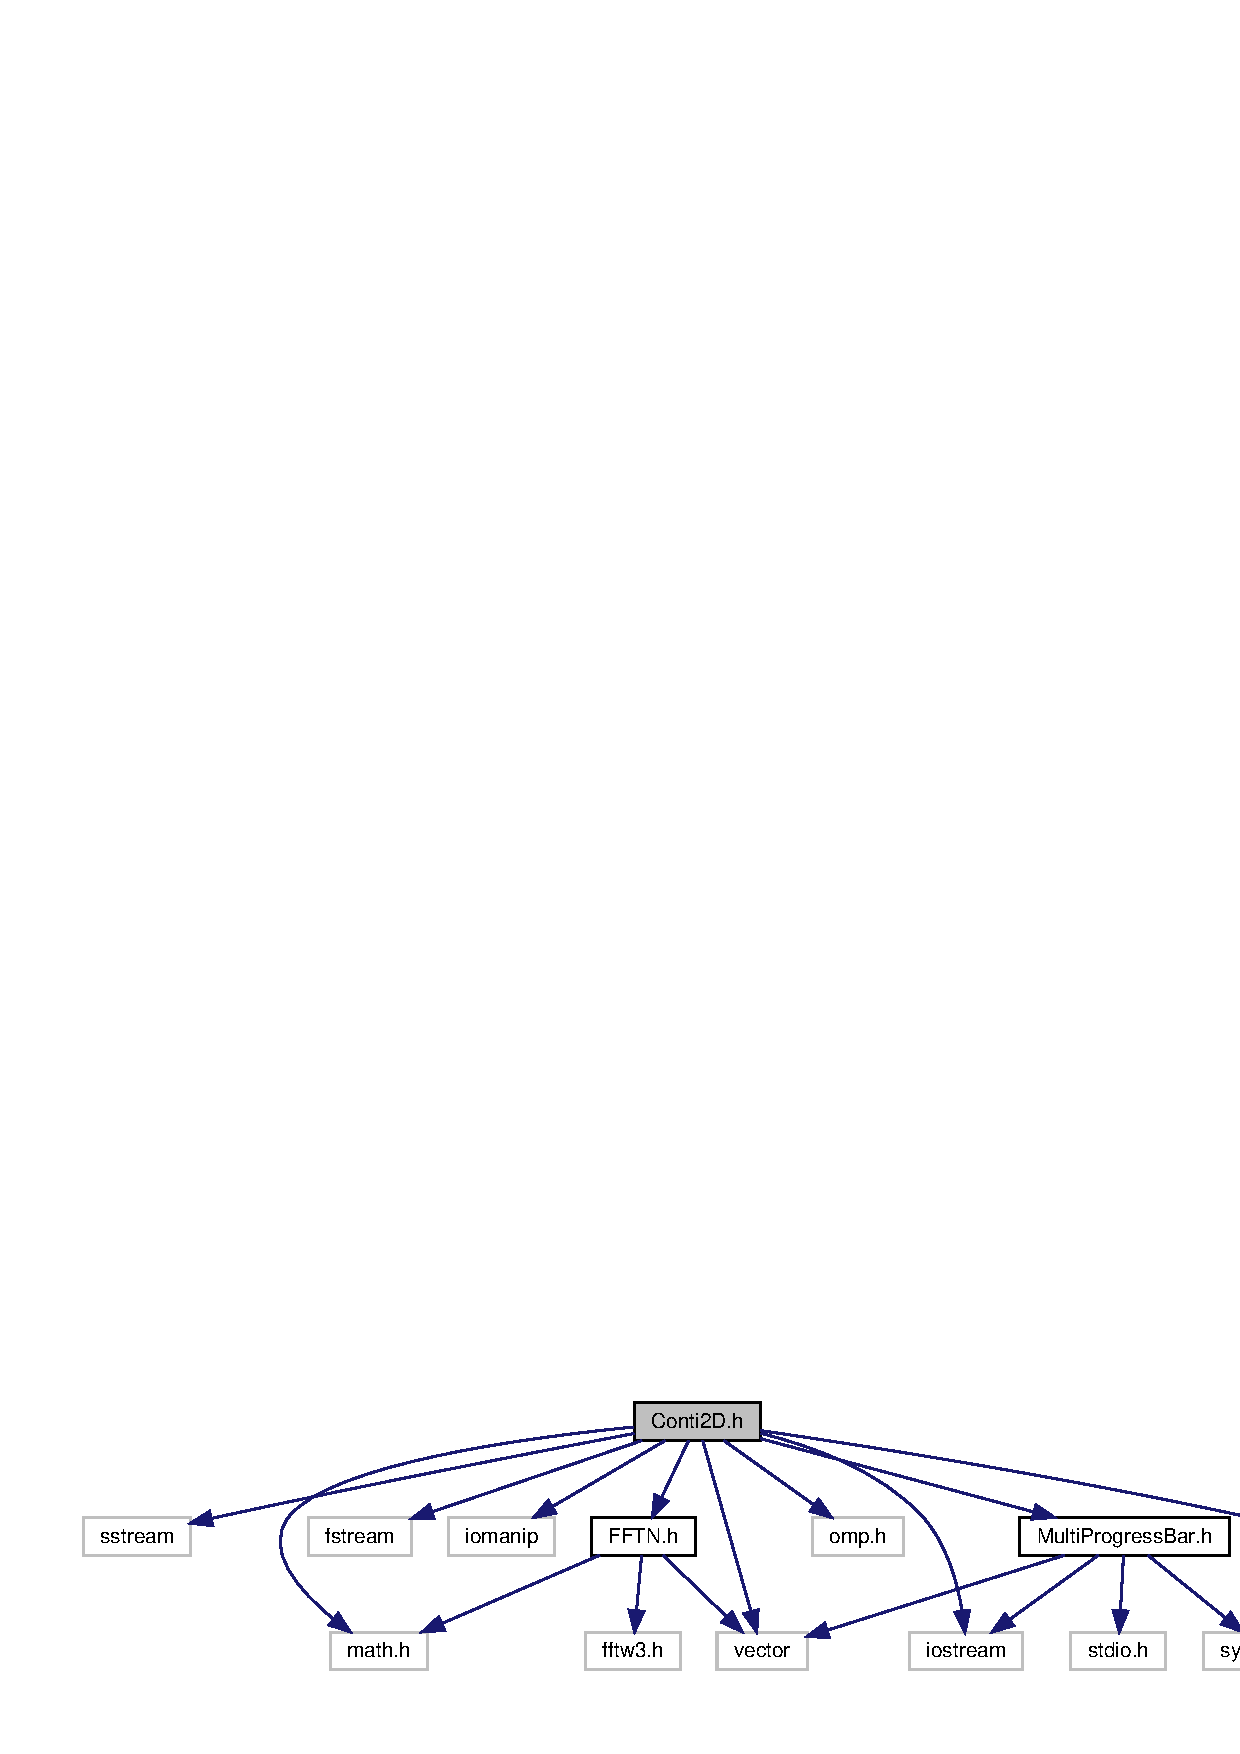
\includegraphics[width=350pt]{Conti2D_8h__incl}
\end{center}
\end{figure}
This graph shows which files directly or indirectly include this file\+:\nopagebreak
\begin{figure}[H]
\begin{center}
\leavevmode
\includegraphics[width=319pt]{Conti2D_8h__dep__incl}
\end{center}
\end{figure}
\subsection*{Classes}
\begin{DoxyCompactItemize}
\item 
struct \textbf{ Grd\+Head}
\begin{DoxyCompactList}\small\item\em head information of a grid data, e.\+g. \end{DoxyCompactList}\end{DoxyCompactItemize}
\subsection*{Macros}
\begin{DoxyCompactItemize}
\item 
\#define \textbf{ PI}~3.\+141592653
\item 
\#define \textbf{ D\+W\+C\+\_\+\+C\+G\+LS}~1
\item 
\#define \textbf{ D\+W\+C\+\_\+\+T\+I\+K\+H\+O\+N\+OV}~2
\item 
\#define \textbf{ D\+W\+C\+\_\+\+I\+N\+T\+E\+G\+R\+A\+L\+I\+T\+E\+R\+A\+T\+I\+ON}~3
\item 
\#define \textbf{ D\+W\+C\+\_\+\+L\+A\+N\+D\+W\+E\+B\+ER}~4
\item 
\#define \textbf{ E\+R\+R\+O\+R\+\_\+\+C\+O\+UT}~\char`\"{}[\char`\"{}$<$$<$\char`\"{}\textbackslash{}033[31m\+Error\char`\"{}$<$$<$\char`\"{}\textbackslash{}033[0m] \char`\"{}
\item 
\#define \textbf{ W\+A\+R\+N\+\_\+\+C\+O\+UT}~\char`\"{}[\char`\"{}$<$$<$\char`\"{}\textbackslash{}033[33m\+Warning\char`\"{}$<$$<$\char`\"{}\textbackslash{}033[0m] \char`\"{}
\item 
\#define \textbf{ E\+R\+R\+O\+R\+\_\+\+C\+O\+UT}~\char`\"{}[\char`\"{}$<$$<$\char`\"{}\textbackslash{}033[31m\+Error\char`\"{}$<$$<$\char`\"{}\textbackslash{}033[0m] \char`\"{}
\item 
\#define \textbf{ P\+U\+R\+P\+LE}~\char`\"{}\textbackslash{}033[35m\char`\"{}
\item 
\#define \textbf{ R\+ED}~\char`\"{}\textbackslash{}033[31m\char`\"{}
\item 
\#define \textbf{ G\+R\+E\+EN}~\char`\"{}\textbackslash{}033[32m\char`\"{}
\item 
\#define \textbf{ Y\+E\+L\+L\+OW}~\char`\"{}\textbackslash{}033[33m\char`\"{}
\item 
\#define \textbf{ B\+L\+UE}~\char`\"{}\textbackslash{}033[34m\char`\"{}
\item 
\#define \textbf{ C\+O\+L\+O\+R\+\_\+\+D\+E\+F\+A\+L\+UT}~\char`\"{}\textbackslash{}033[0m\char`\"{}
\item 
\#define \textbf{ M\+O\+V\+E\+UP}(x)~printf(\char`\"{}\textbackslash{}033[\%dA\char`\"{}, (x))
\item 
\#define \textbf{ C\+L\+E\+AR}()~printf(\char`\"{}\textbackslash{}033[2\+J\char`\"{})
\item 
\#define \textbf{ M\+O\+V\+E\+UP}(x)~printf(\char`\"{}\textbackslash{}033[\%dA\char`\"{}, (x))
\item 
\#define \textbf{ M\+O\+V\+E\+D\+O\+WN}(x)~printf(\char`\"{}\textbackslash{}033[\%dB\char`\"{}, (x))
\item 
\#define \textbf{ M\+O\+V\+E\+L\+E\+FT}(y)~printf(\char`\"{}\textbackslash{}033[\%dD\char`\"{}, (y))
\item 
\#define \textbf{ M\+O\+V\+E\+R\+I\+G\+HT}(y)~printf(\char`\"{}\textbackslash{}033[\%dC\char`\"{},(y))
\item 
\#define \textbf{ M\+O\+V\+E\+TO}(x,  y)~printf(\char`\"{}\textbackslash{}033[\%d;\%dH\char`\"{}, (x), (y))
\item 
\#define \textbf{ R\+E\+S\+E\+T\+\_\+\+C\+U\+R\+S\+OR}()~printf(\char`\"{}\textbackslash{}033[H\char`\"{})
\item 
\#define \textbf{ H\+I\+D\+E\+\_\+\+C\+U\+R\+S\+OR}()~printf(\char`\"{}\textbackslash{}033[?25l\char`\"{})
\item 
\#define \textbf{ S\+H\+O\+W\+\_\+\+C\+U\+R\+S\+OR}()~printf(\char`\"{}\textbackslash{}033[?25h\char`\"{})
\item 
\#define \textbf{ H\+I\+G\+H\+T\+\_\+\+L\+I\+G\+HT}()~printf(\char`\"{}\textbackslash{}033[7m\char`\"{})
\item 
\#define \textbf{ U\+N\+\_\+\+H\+I\+G\+H\+T\+\_\+\+L\+I\+G\+HT}()~printf(\char`\"{}\textbackslash{}033[27m\char`\"{})
\end{DoxyCompactItemize}
\subsection*{Functions}
\begin{DoxyCompactItemize}
\item 
double $\ast$ \textbf{ Read\+Grd} (string filename, \textbf{ Grd\+Head} \&grdhead, int ext\+Num)
\begin{DoxyCompactList}\small\item\em Read a Surfer Grid data from file. \end{DoxyCompactList}\item 
bool \textbf{ Save\+Grd} (string filename, \textbf{ Grd\+Head} grdhead, double $\ast$data, int ext\+Num, bool savexxyz=false, bool is\+Info=true)
\begin{DoxyCompactList}\small\item\em Save a Surfer Grid data to file. \end{DoxyCompactList}\item 
void \textbf{ Get\+Kernal\+Matrix} (\textbf{ Grd\+Head} grdhead, double $\ast$G, const double rph, int num\+\_\+thread=4)
\begin{DoxyCompactList}\small\item\em Get the Kernal Matrix object. \end{DoxyCompactList}\item 
void \textbf{ Get\+Kernal\+Matrix\+\_\+new} (\textbf{ Grd\+Head} grdhead, double $\ast$G, const double rph, int num\+\_\+thread=4)
\begin{DoxyCompactList}\small\item\em Get the kernel matrix using the new developed formula. \end{DoxyCompactList}\item 
double \textbf{ Get\+Gij} (const int i, const int j, double $\ast$first\+Row, const \textbf{ Grd\+Head} grdhead)
\begin{DoxyCompactList}\small\item\em Get the value at i row and the j column of kernel matrix from the first row of the matrix only. \end{DoxyCompactList}\item 
int \textbf{ Getkernel\+\_\+p2p} (\textbf{ Grd\+Head} grdhead, double rph, double $\ast$$\ast$kernel, int num\+\_\+thread)
\begin{DoxyCompactList}\small\item\em Upward continue from plane to plane. \end{DoxyCompactList}\item 
int \textbf{ Getkernel\+\_\+p2p\+\_\+new} (\textbf{ Grd\+Head} grdhead, double rph, double $\ast$kernel\+\_\+first\+Row, int num\+\_\+thread)
\item 
int \textbf{ Getkernel\+\_\+p2p\+\_\+new} (\textbf{ Grd\+Head} grdhead, double rph, double $\ast$$\ast$kernel, int num\+\_\+thread)
\item 
void \textbf{ U\+W\+C\+\_\+p2p} (string inputfilename, string outputfilename, double height1, double height2, int ext\+Num, int num\+\_\+thread, bool is\+Progress, bool use\+Old\+Kernel, string filename\+\_\+exact)
\item 
void \textbf{ U\+W\+C\+\_\+p2p\+\_\+f} (string inputfilename, string outputfilename, double height1, double height2, int ext\+Num, string filename\+\_\+exact)
\item 
int \textbf{ U\+W\+C\+\_\+p2p\+\_\+f} (double $\ast$inputdata, double $\ast$result, \textbf{ Grd\+Head} grdhead, double rph)
\item 
int \textbf{ Getkernel\+\_\+u2p} (\textbf{ Grd\+Head} grdhead, double $\ast$terrain1, double height2, double $\ast$$\ast$kernel, int num\+\_\+thread)
\item 
int \textbf{ Getkernel\+\_\+u2p\+\_\+new} (\textbf{ Grd\+Head} grdhead, double $\ast$terrain1, double height2, double $\ast$nx, double $\ast$ny, double $\ast$nz, double $\ast$$\ast$kernel, int num\+\_\+thread)
\item 
int \textbf{ Getkernel\+\_\+p2s\+\_\+new} (\textbf{ Grd\+Head} grdhead, double h1, double $\ast$topo2, double $\ast$$\ast$kernel, int num\+\_\+thread)
\item 
void \textbf{ Get\+Pmnij} (double $\ast$Pmnij, int rows, int cols, double dx, double dy, double rph, double xm, double ym)
\item 
void \textbf{ U\+WC} (double $\ast$datain, double $\ast$dataout, \textbf{ Grd\+Head} grdhead, double $\ast$$\ast$G)
\item 
void \textbf{ U\+W\+C\+\_\+\+Gij} (double $\ast$b, double $\ast$G, double $\ast$x, \textbf{ Grd\+Head} grdhead, int num\+\_\+thread=1)
\item 
void \textbf{ U\+W\+C\+\_\+\+Gji} (double $\ast$b, double $\ast$G, double $\ast$x, \textbf{ Grd\+Head} grdhead, int num\+\_\+thread=1)
\item 
void \textbf{ U\+W\+C\+\_\+\+Gij} (double $\ast$b, double $\ast$$\ast$G, double $\ast$x, int modelnum, int num\+\_\+thread=1)
\item 
void \textbf{ U\+W\+C\+\_\+\+G\+\_\+\+C\+G\+L\+S\+\_\+\+Tik} (double $\ast$b, double $\ast$$\ast$G, double $\ast$x, int modelnum, double lambda2, int num\+\_\+thread=1)
\item 
void \textbf{ U\+W\+C\+\_\+\+Gji} (double $\ast$b, double $\ast$$\ast$G, double $\ast$x, int modelnum, int num\+\_\+thread=1)
\item 
void \textbf{ D\+W\+C\+\_\+u2p} (string inputfilename, string outputfilename, double height1, string filename\+\_\+topo2)
\item 
void \textbf{ D\+W\+C\+\_\+p2p\+\_\+f} (string inputfilename, string outputfilename, double height1, double height2, int ext\+Num, double T\+RP, int num\+\_\+thread, bool is\+Progress, bool use\+Old\+Kernel)
\item 
void \textbf{ D\+W\+C\+\_\+p2p} (string inputfilename, string outputfilename, double height1, double height2, int ext\+Num, double D\+W\+C\+\_\+parameter, int D\+W\+C\+\_\+method, int num\+\_\+thread, bool is\+Progress, bool use\+Old\+Kernel, string filename\+\_\+exact)
\item 
void \textbf{ U\+W\+C\+\_\+p2s} (string inputfilename, string outputfilename, double height1, string topo\+File, int ext\+Num, int num\+\_\+thread, bool is\+Progress, bool use\+Old\+Kernel, string filename\+\_\+exact)
\item 
void \textbf{ D\+W\+C\+\_\+s2p} (string inputfilename, string outputfilename, string topo1, double height2, int ext\+Num, double D\+W\+C\+\_\+parameter, int D\+W\+C\+\_\+method, int num\+\_\+thread, bool is\+Progress, bool use\+Old\+Kernel, string filename\+\_\+exact)
\item 
void \textbf{ D\+W\+C\+\_\+\+Tikhonov\+\_\+old} (double $\ast$G\+\_\+first\+Row, double $\ast$dataout, double $\ast$indata, double T\+RP, int kmax, double daierta, \textbf{ Grd\+Head} grdhead, int num\+\_\+thread)
\item 
void \textbf{ D\+W\+C\+\_\+p2p\+\_\+\+C\+G\+LS} (double $\ast$G\+\_\+first\+Row, double $\ast$x, double $\ast$b, \textbf{ Grd\+Head} grdhead, int ext\+Num, double delta, int num\+\_\+thread)
\item 
void \textbf{ D\+W\+C\+\_\+s2p\+\_\+\+C\+G\+LS} (double $\ast$$\ast$G, double $\ast$x, double $\ast$b, \textbf{ Grd\+Head} grdhead, int ext\+Num, double delta, int num\+\_\+thread)
\item 
void \textbf{ D\+W\+C\+\_\+s2p\+\_\+\+Tikhonov} (double $\ast$$\ast$G, double $\ast$x, double $\ast$b, \textbf{ Grd\+Head} grdhead, int ext\+Num, double lambda, int num\+\_\+thread)
\item 
void \textbf{ D\+W\+C\+\_\+s2p\+\_\+\+Itegration\+Iter} (double $\ast$$\ast$G, double $\ast$x, double $\ast$b, \textbf{ Grd\+Head} grdhead, int ext\+Num, int num\+\_\+thread, string outputfile, double iter\+\_\+number, double $\ast$Exact\+Solution=N\+U\+LL)
\item 
void \textbf{ D\+W\+C\+\_\+p2p\+\_\+\+Itegration\+Iter} (double $\ast$G, double $\ast$x, double $\ast$b, \textbf{ Grd\+Head} grdhead, int ext\+Num, int num\+\_\+thread, string outputfile, double iter\+\_\+number, double $\ast$Exact\+Solution=N\+U\+LL)
\item 
void \textbf{ D\+W\+C\+\_\+p2p\+\_\+\+Landweber\+Iter} (double $\ast$G, double $\ast$x, double $\ast$b, \textbf{ Grd\+Head} grdhead, int ext\+Num, int num\+\_\+thread, string outputfile, double iter\+\_\+number, double $\ast$Exact\+Solution=N\+U\+LL)
\item 
void \textbf{ D\+W\+C\+\_\+s2p\+\_\+\+Landweber\+Iter} (double $\ast$$\ast$G, double $\ast$x, double $\ast$b, \textbf{ Grd\+Head} grdhead, int ext\+Num, int num\+\_\+thread, string outputfile, double iter\+\_\+number, double $\ast$Exact\+Solution=N\+U\+LL)
\item 
double \textbf{ Norm2} (double $\ast$x, const int num)
\item 
string \textbf{ Path\+\_\+\+Get\+Base\+Name} (string filepath)
\item 
string \textbf{ Path\+\_\+\+Get\+Ext\+Name} (string filepath)
\item 
string \textbf{ Path\+\_\+\+Get\+Path} (string filepath)
\item 
string \textbf{ Path\+\_\+\+Get\+File\+Name} (string filepath)
\item 
double \textbf{ Norm2\+\_\+\+Gradient} (double $\ast$result, \textbf{ Grd\+Head} grdhead)
\item 
int \textbf{ Save\+Grd2\+V\+TK} (string outputfile, \textbf{ Grd\+Head} grdhead, double $\ast$data)
\item 
static void \textbf{ Start\+Text} ()
\item 
static void \textbf{ Text\+\_\+\+Axis} ()
\item 
static void \textbf{ help\+I\+N\+FO} ()
\item 
static void \textbf{ Start\+Text\+\_\+art\+A\+S\+C\+II} ()
\item 
static void \textbf{ Output\+Errorinfo} (string info)
\item 
static void \textbf{ Output\+Warninginfo} (string info)
\end{DoxyCompactItemize}


\subsection{Macro Definition Documentation}
\mbox{\label{Conti2D_8h_a79d10e672abb49ad63eeaa8aaef57c38_a79d10e672abb49ad63eeaa8aaef57c38}} 
\index{Conti2\+D.\+h@{Conti2\+D.\+h}!B\+L\+UE@{B\+L\+UE}}
\index{B\+L\+UE@{B\+L\+UE}!Conti2\+D.\+h@{Conti2\+D.\+h}}
\subsubsection{B\+L\+UE}
{\footnotesize\ttfamily \#define B\+L\+UE~\char`\"{}\textbackslash{}033[34m\char`\"{}}



Definition at line 35 of file Conti2\+D.\+h.



Referenced by Read\+Grd().

\mbox{\label{Conti2D_8h_aacb71dbc63837c5e60f70180643354b2_aacb71dbc63837c5e60f70180643354b2}} 
\index{Conti2\+D.\+h@{Conti2\+D.\+h}!C\+L\+E\+AR@{C\+L\+E\+AR}}
\index{C\+L\+E\+AR@{C\+L\+E\+AR}!Conti2\+D.\+h@{Conti2\+D.\+h}}
\subsubsection{C\+L\+E\+AR}
{\footnotesize\ttfamily \#define C\+L\+E\+AR(\begin{DoxyParamCaption}{ }\end{DoxyParamCaption})~printf(\char`\"{}\textbackslash{}033[2\+J\char`\"{})}



Definition at line 40 of file Conti2\+D.\+h.

\mbox{\label{Conti2D_8h_aa07f331bc3ea046a7f2b28f487d6dfdb_aa07f331bc3ea046a7f2b28f487d6dfdb}} 
\index{Conti2\+D.\+h@{Conti2\+D.\+h}!C\+O\+L\+O\+R\+\_\+\+D\+E\+F\+A\+L\+UT@{C\+O\+L\+O\+R\+\_\+\+D\+E\+F\+A\+L\+UT}}
\index{C\+O\+L\+O\+R\+\_\+\+D\+E\+F\+A\+L\+UT@{C\+O\+L\+O\+R\+\_\+\+D\+E\+F\+A\+L\+UT}!Conti2\+D.\+h@{Conti2\+D.\+h}}
\subsubsection{C\+O\+L\+O\+R\+\_\+\+D\+E\+F\+A\+L\+UT}
{\footnotesize\ttfamily \#define C\+O\+L\+O\+R\+\_\+\+D\+E\+F\+A\+L\+UT~\char`\"{}\textbackslash{}033[0m\char`\"{}}



Definition at line 36 of file Conti2\+D.\+h.



Referenced by D\+W\+C\+\_\+p2p(), D\+W\+C\+\_\+p2p\+\_\+\+Itegration\+Iter(), D\+W\+C\+\_\+p2p\+\_\+\+Landweber\+Iter(), D\+W\+C\+\_\+s2p(), D\+W\+C\+\_\+s2p\+\_\+\+Itegration\+Iter(), D\+W\+C\+\_\+s2p\+\_\+\+Landweber\+Iter(), help\+I\+N\+F\+O(), main(), Read\+Grd(), Save\+Grd(), Save\+Grd2\+V\+T\+K(), Start\+Text\+\_\+art\+A\+S\+C\+I\+I(), Multi\+Progress\+Bar\+::\+Update(), and U\+W\+C\+\_\+p2s().

\mbox{\label{Conti2D_8h_aa1811514ed34916c0a8294b82af37cdd_aa1811514ed34916c0a8294b82af37cdd}} 
\index{Conti2\+D.\+h@{Conti2\+D.\+h}!D\+W\+C\+\_\+\+C\+G\+LS@{D\+W\+C\+\_\+\+C\+G\+LS}}
\index{D\+W\+C\+\_\+\+C\+G\+LS@{D\+W\+C\+\_\+\+C\+G\+LS}!Conti2\+D.\+h@{Conti2\+D.\+h}}
\subsubsection{D\+W\+C\+\_\+\+C\+G\+LS}
{\footnotesize\ttfamily \#define D\+W\+C\+\_\+\+C\+G\+LS~1}



Definition at line 23 of file Conti2\+D.\+h.



Referenced by D\+W\+C\+\_\+p2p(), D\+W\+C\+\_\+s2p(), and main().

\mbox{\label{Conti2D_8h_abd93919e7f5a6527a31eeee1fe07c9b2_abd93919e7f5a6527a31eeee1fe07c9b2}} 
\index{Conti2\+D.\+h@{Conti2\+D.\+h}!D\+W\+C\+\_\+\+I\+N\+T\+E\+G\+R\+A\+L\+I\+T\+E\+R\+A\+T\+I\+ON@{D\+W\+C\+\_\+\+I\+N\+T\+E\+G\+R\+A\+L\+I\+T\+E\+R\+A\+T\+I\+ON}}
\index{D\+W\+C\+\_\+\+I\+N\+T\+E\+G\+R\+A\+L\+I\+T\+E\+R\+A\+T\+I\+ON@{D\+W\+C\+\_\+\+I\+N\+T\+E\+G\+R\+A\+L\+I\+T\+E\+R\+A\+T\+I\+ON}!Conti2\+D.\+h@{Conti2\+D.\+h}}
\subsubsection{D\+W\+C\+\_\+\+I\+N\+T\+E\+G\+R\+A\+L\+I\+T\+E\+R\+A\+T\+I\+ON}
{\footnotesize\ttfamily \#define D\+W\+C\+\_\+\+I\+N\+T\+E\+G\+R\+A\+L\+I\+T\+E\+R\+A\+T\+I\+ON~3}



Definition at line 25 of file Conti2\+D.\+h.



Referenced by D\+W\+C\+\_\+p2p(), D\+W\+C\+\_\+s2p(), and main().

\mbox{\label{Conti2D_8h_a627da9b3aee3cd273e34d3675cb95e49_a627da9b3aee3cd273e34d3675cb95e49}} 
\index{Conti2\+D.\+h@{Conti2\+D.\+h}!D\+W\+C\+\_\+\+L\+A\+N\+D\+W\+E\+B\+ER@{D\+W\+C\+\_\+\+L\+A\+N\+D\+W\+E\+B\+ER}}
\index{D\+W\+C\+\_\+\+L\+A\+N\+D\+W\+E\+B\+ER@{D\+W\+C\+\_\+\+L\+A\+N\+D\+W\+E\+B\+ER}!Conti2\+D.\+h@{Conti2\+D.\+h}}
\subsubsection{D\+W\+C\+\_\+\+L\+A\+N\+D\+W\+E\+B\+ER}
{\footnotesize\ttfamily \#define D\+W\+C\+\_\+\+L\+A\+N\+D\+W\+E\+B\+ER~4}



Definition at line 26 of file Conti2\+D.\+h.



Referenced by D\+W\+C\+\_\+p2p(), D\+W\+C\+\_\+s2p(), and main().

\mbox{\label{Conti2D_8h_a600e2a1b514c2a21a9ce3e97637b65ae_a600e2a1b514c2a21a9ce3e97637b65ae}} 
\index{Conti2\+D.\+h@{Conti2\+D.\+h}!D\+W\+C\+\_\+\+T\+I\+K\+H\+O\+N\+OV@{D\+W\+C\+\_\+\+T\+I\+K\+H\+O\+N\+OV}}
\index{D\+W\+C\+\_\+\+T\+I\+K\+H\+O\+N\+OV@{D\+W\+C\+\_\+\+T\+I\+K\+H\+O\+N\+OV}!Conti2\+D.\+h@{Conti2\+D.\+h}}
\subsubsection{D\+W\+C\+\_\+\+T\+I\+K\+H\+O\+N\+OV}
{\footnotesize\ttfamily \#define D\+W\+C\+\_\+\+T\+I\+K\+H\+O\+N\+OV~2}



Definition at line 24 of file Conti2\+D.\+h.



Referenced by D\+W\+C\+\_\+p2p(), D\+W\+C\+\_\+s2p(), and main().

\mbox{\label{Conti2D_8h_a6200c444a92cd12d31ac6bdaf7c221d0_a6200c444a92cd12d31ac6bdaf7c221d0}} 
\index{Conti2\+D.\+h@{Conti2\+D.\+h}!E\+R\+R\+O\+R\+\_\+\+C\+O\+UT@{E\+R\+R\+O\+R\+\_\+\+C\+O\+UT}}
\index{E\+R\+R\+O\+R\+\_\+\+C\+O\+UT@{E\+R\+R\+O\+R\+\_\+\+C\+O\+UT}!Conti2\+D.\+h@{Conti2\+D.\+h}}
\subsubsection{E\+R\+R\+O\+R\+\_\+\+C\+O\+UT\hspace{0.1cm}{\footnotesize\ttfamily [1/2]}}
{\footnotesize\ttfamily \#define E\+R\+R\+O\+R\+\_\+\+C\+O\+UT~\char`\"{}[\char`\"{}$<$$<$\char`\"{}\textbackslash{}033[31m\+Error\char`\"{}$<$$<$\char`\"{}\textbackslash{}033[0m] \char`\"{}}



Definition at line 30 of file Conti2\+D.\+h.

\mbox{\label{Conti2D_8h_a6200c444a92cd12d31ac6bdaf7c221d0_a6200c444a92cd12d31ac6bdaf7c221d0}} 
\index{Conti2\+D.\+h@{Conti2\+D.\+h}!E\+R\+R\+O\+R\+\_\+\+C\+O\+UT@{E\+R\+R\+O\+R\+\_\+\+C\+O\+UT}}
\index{E\+R\+R\+O\+R\+\_\+\+C\+O\+UT@{E\+R\+R\+O\+R\+\_\+\+C\+O\+UT}!Conti2\+D.\+h@{Conti2\+D.\+h}}
\subsubsection{E\+R\+R\+O\+R\+\_\+\+C\+O\+UT\hspace{0.1cm}{\footnotesize\ttfamily [2/2]}}
{\footnotesize\ttfamily \#define E\+R\+R\+O\+R\+\_\+\+C\+O\+UT~\char`\"{}[\char`\"{}$<$$<$\char`\"{}\textbackslash{}033[31m\+Error\char`\"{}$<$$<$\char`\"{}\textbackslash{}033[0m] \char`\"{}}



Definition at line 30 of file Conti2\+D.\+h.

\mbox{\label{Conti2D_8h_acfbc006ea433ad708fdee3e82996e721_acfbc006ea433ad708fdee3e82996e721}} 
\index{Conti2\+D.\+h@{Conti2\+D.\+h}!G\+R\+E\+EN@{G\+R\+E\+EN}}
\index{G\+R\+E\+EN@{G\+R\+E\+EN}!Conti2\+D.\+h@{Conti2\+D.\+h}}
\subsubsection{G\+R\+E\+EN}
{\footnotesize\ttfamily \#define G\+R\+E\+EN~\char`\"{}\textbackslash{}033[32m\char`\"{}}



Definition at line 33 of file Conti2\+D.\+h.



Referenced by D\+W\+C\+\_\+p2p\+\_\+\+Itegration\+Iter(), D\+W\+C\+\_\+p2p\+\_\+\+Landweber\+Iter(), D\+W\+C\+\_\+s2p\+\_\+\+Itegration\+Iter(), D\+W\+C\+\_\+s2p\+\_\+\+Landweber\+Iter(), help\+I\+N\+F\+O(), Read\+Grd(), Save\+Grd(), and Start\+Text\+\_\+art\+A\+S\+C\+I\+I().

\mbox{\label{Conti2D_8h_afda389c3c8b482e025dc765d250a5a0d_afda389c3c8b482e025dc765d250a5a0d}} 
\index{Conti2\+D.\+h@{Conti2\+D.\+h}!H\+I\+D\+E\+\_\+\+C\+U\+R\+S\+OR@{H\+I\+D\+E\+\_\+\+C\+U\+R\+S\+OR}}
\index{H\+I\+D\+E\+\_\+\+C\+U\+R\+S\+OR@{H\+I\+D\+E\+\_\+\+C\+U\+R\+S\+OR}!Conti2\+D.\+h@{Conti2\+D.\+h}}
\subsubsection{H\+I\+D\+E\+\_\+\+C\+U\+R\+S\+OR}
{\footnotesize\ttfamily \#define H\+I\+D\+E\+\_\+\+C\+U\+R\+S\+OR(\begin{DoxyParamCaption}{ }\end{DoxyParamCaption})~printf(\char`\"{}\textbackslash{}033[?25l\char`\"{})}



Definition at line 54 of file Conti2\+D.\+h.

\mbox{\label{Conti2D_8h_abcf37352db560ac79462be29a1e5d2f9_abcf37352db560ac79462be29a1e5d2f9}} 
\index{Conti2\+D.\+h@{Conti2\+D.\+h}!H\+I\+G\+H\+T\+\_\+\+L\+I\+G\+HT@{H\+I\+G\+H\+T\+\_\+\+L\+I\+G\+HT}}
\index{H\+I\+G\+H\+T\+\_\+\+L\+I\+G\+HT@{H\+I\+G\+H\+T\+\_\+\+L\+I\+G\+HT}!Conti2\+D.\+h@{Conti2\+D.\+h}}
\subsubsection{H\+I\+G\+H\+T\+\_\+\+L\+I\+G\+HT}
{\footnotesize\ttfamily \#define H\+I\+G\+H\+T\+\_\+\+L\+I\+G\+HT(\begin{DoxyParamCaption}{ }\end{DoxyParamCaption})~printf(\char`\"{}\textbackslash{}033[7m\char`\"{})}



Definition at line 57 of file Conti2\+D.\+h.

\mbox{\label{Conti2D_8h_a60c20a6d25d201dedc09459516728b71_a60c20a6d25d201dedc09459516728b71}} 
\index{Conti2\+D.\+h@{Conti2\+D.\+h}!M\+O\+V\+E\+D\+O\+WN@{M\+O\+V\+E\+D\+O\+WN}}
\index{M\+O\+V\+E\+D\+O\+WN@{M\+O\+V\+E\+D\+O\+WN}!Conti2\+D.\+h@{Conti2\+D.\+h}}
\subsubsection{M\+O\+V\+E\+D\+O\+WN}
{\footnotesize\ttfamily \#define M\+O\+V\+E\+D\+O\+WN(\begin{DoxyParamCaption}\item[{}]{x }\end{DoxyParamCaption})~printf(\char`\"{}\textbackslash{}033[\%dB\char`\"{}, (x))}



Definition at line 44 of file Conti2\+D.\+h.

\mbox{\label{Conti2D_8h_aa4013bd7c760612afc0aae84427d1830_aa4013bd7c760612afc0aae84427d1830}} 
\index{Conti2\+D.\+h@{Conti2\+D.\+h}!M\+O\+V\+E\+L\+E\+FT@{M\+O\+V\+E\+L\+E\+FT}}
\index{M\+O\+V\+E\+L\+E\+FT@{M\+O\+V\+E\+L\+E\+FT}!Conti2\+D.\+h@{Conti2\+D.\+h}}
\subsubsection{M\+O\+V\+E\+L\+E\+FT}
{\footnotesize\ttfamily \#define M\+O\+V\+E\+L\+E\+FT(\begin{DoxyParamCaption}\item[{}]{y }\end{DoxyParamCaption})~printf(\char`\"{}\textbackslash{}033[\%dD\char`\"{}, (y))}



Definition at line 46 of file Conti2\+D.\+h.

\mbox{\label{Conti2D_8h_a04d744faff56ecc898524480a76747b8_a04d744faff56ecc898524480a76747b8}} 
\index{Conti2\+D.\+h@{Conti2\+D.\+h}!M\+O\+V\+E\+R\+I\+G\+HT@{M\+O\+V\+E\+R\+I\+G\+HT}}
\index{M\+O\+V\+E\+R\+I\+G\+HT@{M\+O\+V\+E\+R\+I\+G\+HT}!Conti2\+D.\+h@{Conti2\+D.\+h}}
\subsubsection{M\+O\+V\+E\+R\+I\+G\+HT}
{\footnotesize\ttfamily \#define M\+O\+V\+E\+R\+I\+G\+HT(\begin{DoxyParamCaption}\item[{}]{y }\end{DoxyParamCaption})~printf(\char`\"{}\textbackslash{}033[\%dC\char`\"{},(y))}



Definition at line 48 of file Conti2\+D.\+h.

\mbox{\label{Conti2D_8h_a0d378f5b71290eff0a6252149f0e311e_a0d378f5b71290eff0a6252149f0e311e}} 
\index{Conti2\+D.\+h@{Conti2\+D.\+h}!M\+O\+V\+E\+TO@{M\+O\+V\+E\+TO}}
\index{M\+O\+V\+E\+TO@{M\+O\+V\+E\+TO}!Conti2\+D.\+h@{Conti2\+D.\+h}}
\subsubsection{M\+O\+V\+E\+TO}
{\footnotesize\ttfamily \#define M\+O\+V\+E\+TO(\begin{DoxyParamCaption}\item[{}]{x,  }\item[{}]{y }\end{DoxyParamCaption})~printf(\char`\"{}\textbackslash{}033[\%d;\%dH\char`\"{}, (x), (y))}



Definition at line 50 of file Conti2\+D.\+h.

\mbox{\label{Conti2D_8h_a39d49b877205e65853206f931e5c2e75_a39d49b877205e65853206f931e5c2e75}} 
\index{Conti2\+D.\+h@{Conti2\+D.\+h}!M\+O\+V\+E\+UP@{M\+O\+V\+E\+UP}}
\index{M\+O\+V\+E\+UP@{M\+O\+V\+E\+UP}!Conti2\+D.\+h@{Conti2\+D.\+h}}
\subsubsection{M\+O\+V\+E\+UP\hspace{0.1cm}{\footnotesize\ttfamily [1/2]}}
{\footnotesize\ttfamily \#define M\+O\+V\+E\+UP(\begin{DoxyParamCaption}\item[{}]{x }\end{DoxyParamCaption})~printf(\char`\"{}\textbackslash{}033[\%dA\char`\"{}, (x))}



Definition at line 42 of file Conti2\+D.\+h.



Referenced by Multi\+Progress\+Bar\+::\+Update().

\mbox{\label{Conti2D_8h_a39d49b877205e65853206f931e5c2e75_a39d49b877205e65853206f931e5c2e75}} 
\index{Conti2\+D.\+h@{Conti2\+D.\+h}!M\+O\+V\+E\+UP@{M\+O\+V\+E\+UP}}
\index{M\+O\+V\+E\+UP@{M\+O\+V\+E\+UP}!Conti2\+D.\+h@{Conti2\+D.\+h}}
\subsubsection{M\+O\+V\+E\+UP\hspace{0.1cm}{\footnotesize\ttfamily [2/2]}}
{\footnotesize\ttfamily \#define M\+O\+V\+E\+UP(\begin{DoxyParamCaption}\item[{}]{x }\end{DoxyParamCaption})~printf(\char`\"{}\textbackslash{}033[\%dA\char`\"{}, (x))}



Definition at line 42 of file Conti2\+D.\+h.

\mbox{\label{Conti2D_8h_a598a3330b3c21701223ee0ca14316eca_a598a3330b3c21701223ee0ca14316eca}} 
\index{Conti2\+D.\+h@{Conti2\+D.\+h}!PI@{PI}}
\index{PI@{PI}!Conti2\+D.\+h@{Conti2\+D.\+h}}
\subsubsection{PI}
{\footnotesize\ttfamily \#define PI~3.\+141592653}



Definition at line 21 of file Conti2\+D.\+h.



Referenced by Get\+Kernal\+Matrix(), Get\+Kernal\+Matrix\+\_\+new(), Getkernel\+\_\+p2p(), Getkernel\+\_\+u2p(), Getkernel\+\_\+u2p\+\_\+new(), Get\+Pmnij(), and U\+W\+C\+\_\+p2p\+\_\+f().

\mbox{\label{Conti2D_8h_a0bb0b009e7a7390473ace4d98bd843c0_a0bb0b009e7a7390473ace4d98bd843c0}} 
\index{Conti2\+D.\+h@{Conti2\+D.\+h}!P\+U\+R\+P\+LE@{P\+U\+R\+P\+LE}}
\index{P\+U\+R\+P\+LE@{P\+U\+R\+P\+LE}!Conti2\+D.\+h@{Conti2\+D.\+h}}
\subsubsection{P\+U\+R\+P\+LE}
{\footnotesize\ttfamily \#define P\+U\+R\+P\+LE~\char`\"{}\textbackslash{}033[35m\char`\"{}}



Definition at line 31 of file Conti2\+D.\+h.



Referenced by help\+I\+N\+F\+O().

\mbox{\label{Conti2D_8h_a8d23feea868a983c8c2b661e1e16972f_a8d23feea868a983c8c2b661e1e16972f}} 
\index{Conti2\+D.\+h@{Conti2\+D.\+h}!R\+ED@{R\+ED}}
\index{R\+ED@{R\+ED}!Conti2\+D.\+h@{Conti2\+D.\+h}}
\subsubsection{R\+ED}
{\footnotesize\ttfamily \#define R\+ED~\char`\"{}\textbackslash{}033[31m\char`\"{}}



Definition at line 32 of file Conti2\+D.\+h.



Referenced by D\+W\+C\+\_\+p2p(), D\+W\+C\+\_\+p2p\+\_\+\+Itegration\+Iter(), D\+W\+C\+\_\+p2p\+\_\+\+Landweber\+Iter(), D\+W\+C\+\_\+s2p(), D\+W\+C\+\_\+s2p\+\_\+\+Itegration\+Iter(), D\+W\+C\+\_\+s2p\+\_\+\+Landweber\+Iter(), main(), Read\+Grd(), Save\+Grd2\+V\+T\+K(), and U\+W\+C\+\_\+p2s().

\mbox{\label{Conti2D_8h_a7c3dbb2345379003d264cc94aeda5f6c_a7c3dbb2345379003d264cc94aeda5f6c}} 
\index{Conti2\+D.\+h@{Conti2\+D.\+h}!R\+E\+S\+E\+T\+\_\+\+C\+U\+R\+S\+OR@{R\+E\+S\+E\+T\+\_\+\+C\+U\+R\+S\+OR}}
\index{R\+E\+S\+E\+T\+\_\+\+C\+U\+R\+S\+OR@{R\+E\+S\+E\+T\+\_\+\+C\+U\+R\+S\+OR}!Conti2\+D.\+h@{Conti2\+D.\+h}}
\subsubsection{R\+E\+S\+E\+T\+\_\+\+C\+U\+R\+S\+OR}
{\footnotesize\ttfamily \#define R\+E\+S\+E\+T\+\_\+\+C\+U\+R\+S\+OR(\begin{DoxyParamCaption}{ }\end{DoxyParamCaption})~printf(\char`\"{}\textbackslash{}033[H\char`\"{})}



Definition at line 52 of file Conti2\+D.\+h.

\mbox{\label{Conti2D_8h_ade9c2a563b11982d9d657d3ac3a0ceb1_ade9c2a563b11982d9d657d3ac3a0ceb1}} 
\index{Conti2\+D.\+h@{Conti2\+D.\+h}!S\+H\+O\+W\+\_\+\+C\+U\+R\+S\+OR@{S\+H\+O\+W\+\_\+\+C\+U\+R\+S\+OR}}
\index{S\+H\+O\+W\+\_\+\+C\+U\+R\+S\+OR@{S\+H\+O\+W\+\_\+\+C\+U\+R\+S\+OR}!Conti2\+D.\+h@{Conti2\+D.\+h}}
\subsubsection{S\+H\+O\+W\+\_\+\+C\+U\+R\+S\+OR}
{\footnotesize\ttfamily \#define S\+H\+O\+W\+\_\+\+C\+U\+R\+S\+OR(\begin{DoxyParamCaption}{ }\end{DoxyParamCaption})~printf(\char`\"{}\textbackslash{}033[?25h\char`\"{})}



Definition at line 56 of file Conti2\+D.\+h.

\mbox{\label{Conti2D_8h_ab97f6b5de02db4483a7d6bb9bc0c75c0_ab97f6b5de02db4483a7d6bb9bc0c75c0}} 
\index{Conti2\+D.\+h@{Conti2\+D.\+h}!U\+N\+\_\+\+H\+I\+G\+H\+T\+\_\+\+L\+I\+G\+HT@{U\+N\+\_\+\+H\+I\+G\+H\+T\+\_\+\+L\+I\+G\+HT}}
\index{U\+N\+\_\+\+H\+I\+G\+H\+T\+\_\+\+L\+I\+G\+HT@{U\+N\+\_\+\+H\+I\+G\+H\+T\+\_\+\+L\+I\+G\+HT}!Conti2\+D.\+h@{Conti2\+D.\+h}}
\subsubsection{U\+N\+\_\+\+H\+I\+G\+H\+T\+\_\+\+L\+I\+G\+HT}
{\footnotesize\ttfamily \#define U\+N\+\_\+\+H\+I\+G\+H\+T\+\_\+\+L\+I\+G\+HT(\begin{DoxyParamCaption}{ }\end{DoxyParamCaption})~printf(\char`\"{}\textbackslash{}033[27m\char`\"{})}



Definition at line 58 of file Conti2\+D.\+h.

\mbox{\label{Conti2D_8h_a624c50676f68bfc5c188e83c1fb102d3_a624c50676f68bfc5c188e83c1fb102d3}} 
\index{Conti2\+D.\+h@{Conti2\+D.\+h}!W\+A\+R\+N\+\_\+\+C\+O\+UT@{W\+A\+R\+N\+\_\+\+C\+O\+UT}}
\index{W\+A\+R\+N\+\_\+\+C\+O\+UT@{W\+A\+R\+N\+\_\+\+C\+O\+UT}!Conti2\+D.\+h@{Conti2\+D.\+h}}
\subsubsection{W\+A\+R\+N\+\_\+\+C\+O\+UT}
{\footnotesize\ttfamily \#define W\+A\+R\+N\+\_\+\+C\+O\+UT~\char`\"{}[\char`\"{}$<$$<$\char`\"{}\textbackslash{}033[33m\+Warning\char`\"{}$<$$<$\char`\"{}\textbackslash{}033[0m] \char`\"{}}



Definition at line 29 of file Conti2\+D.\+h.

\mbox{\label{Conti2D_8h_abf681265909adf3d3e8116c93c0ba179_abf681265909adf3d3e8116c93c0ba179}} 
\index{Conti2\+D.\+h@{Conti2\+D.\+h}!Y\+E\+L\+L\+OW@{Y\+E\+L\+L\+OW}}
\index{Y\+E\+L\+L\+OW@{Y\+E\+L\+L\+OW}!Conti2\+D.\+h@{Conti2\+D.\+h}}
\subsubsection{Y\+E\+L\+L\+OW}
{\footnotesize\ttfamily \#define Y\+E\+L\+L\+OW~\char`\"{}\textbackslash{}033[33m\char`\"{}}



Definition at line 34 of file Conti2\+D.\+h.



\subsection{Function Documentation}
\mbox{\label{Conti2D_8h_ab87ce573de93575b7ece2e4f772e03fd_ab87ce573de93575b7ece2e4f772e03fd}} 
\index{Conti2\+D.\+h@{Conti2\+D.\+h}!D\+W\+C\+\_\+p2p@{D\+W\+C\+\_\+p2p}}
\index{D\+W\+C\+\_\+p2p@{D\+W\+C\+\_\+p2p}!Conti2\+D.\+h@{Conti2\+D.\+h}}
\subsubsection{D\+W\+C\+\_\+p2p()}
{\footnotesize\ttfamily void D\+W\+C\+\_\+p2p (\begin{DoxyParamCaption}\item[{string}]{inputfilename,  }\item[{string}]{outputfilename,  }\item[{double}]{height1,  }\item[{double}]{height2,  }\item[{int}]{ext\+Num,  }\item[{double}]{D\+W\+C\+\_\+parameter,  }\item[{int}]{D\+W\+C\+\_\+method,  }\item[{int}]{num\+\_\+thread,  }\item[{bool}]{is\+Progress,  }\item[{bool}]{use\+Old\+Kernel,  }\item[{string}]{filename\+\_\+exact }\end{DoxyParamCaption})}



Definition at line 1669 of file Conti2\+D.\+cpp.



References Grd\+Head\+::bounds, C\+O\+L\+O\+R\+\_\+\+D\+E\+F\+A\+L\+UT, Grd\+Head\+::cols, D\+W\+C\+\_\+\+C\+G\+LS, D\+W\+C\+\_\+\+I\+N\+T\+E\+G\+R\+A\+L\+I\+T\+E\+R\+A\+T\+I\+ON, D\+W\+C\+\_\+\+L\+A\+N\+D\+W\+E\+B\+ER, D\+W\+C\+\_\+s2p\+\_\+\+C\+G\+L\+S(), D\+W\+C\+\_\+s2p\+\_\+\+Itegration\+Iter(), D\+W\+C\+\_\+s2p\+\_\+\+Landweber\+Iter(), D\+W\+C\+\_\+\+T\+I\+K\+H\+O\+N\+OV, Getkernel\+\_\+p2p\+\_\+new(), Read\+Grd(), R\+ED, Grd\+Head\+::rows, and Save\+Grd().



Referenced by main().

Here is the call graph for this function\+:
\nopagebreak
\begin{figure}[H]
\begin{center}
\leavevmode
\includegraphics[width=350pt]{Conti2D_8h_ab87ce573de93575b7ece2e4f772e03fd_ab87ce573de93575b7ece2e4f772e03fd_cgraph}
\end{center}
\end{figure}
Here is the caller graph for this function\+:\nopagebreak
\begin{figure}[H]
\begin{center}
\leavevmode
\includegraphics[width=180pt]{Conti2D_8h_ab87ce573de93575b7ece2e4f772e03fd_ab87ce573de93575b7ece2e4f772e03fd_icgraph}
\end{center}
\end{figure}
\mbox{\label{Conti2D_8h_a68e9e4a8817a29dce16c782fa8213faa_a68e9e4a8817a29dce16c782fa8213faa}} 
\index{Conti2\+D.\+h@{Conti2\+D.\+h}!D\+W\+C\+\_\+p2p\+\_\+\+C\+G\+LS@{D\+W\+C\+\_\+p2p\+\_\+\+C\+G\+LS}}
\index{D\+W\+C\+\_\+p2p\+\_\+\+C\+G\+LS@{D\+W\+C\+\_\+p2p\+\_\+\+C\+G\+LS}!Conti2\+D.\+h@{Conti2\+D.\+h}}
\subsubsection{D\+W\+C\+\_\+p2p\+\_\+\+C\+G\+L\+S()}
{\footnotesize\ttfamily void D\+W\+C\+\_\+p2p\+\_\+\+C\+G\+LS (\begin{DoxyParamCaption}\item[{double $\ast$}]{G\+\_\+first\+Row,  }\item[{double $\ast$}]{x,  }\item[{double $\ast$}]{b,  }\item[{\textbf{ Grd\+Head}}]{grdhead,  }\item[{int}]{ext\+Num,  }\item[{double}]{delta,  }\item[{int}]{num\+\_\+thread }\end{DoxyParamCaption})}



Definition at line 1402 of file Conti2\+D.\+cpp.



References Grd\+Head\+::cols, Norm2(), Grd\+Head\+::rows, Save\+Grd(), Multi\+Progress\+Bar\+::\+Update(), U\+W\+C\+\_\+\+Gij(), and U\+W\+C\+\_\+\+Gji().

Here is the call graph for this function\+:
\nopagebreak
\begin{figure}[H]
\begin{center}
\leavevmode
\includegraphics[width=305pt]{Conti2D_8h_a68e9e4a8817a29dce16c782fa8213faa_a68e9e4a8817a29dce16c782fa8213faa_cgraph}
\end{center}
\end{figure}
\mbox{\label{Conti2D_8h_afb187c363388d28caa8a055176269f12_afb187c363388d28caa8a055176269f12}} 
\index{Conti2\+D.\+h@{Conti2\+D.\+h}!D\+W\+C\+\_\+p2p\+\_\+f@{D\+W\+C\+\_\+p2p\+\_\+f}}
\index{D\+W\+C\+\_\+p2p\+\_\+f@{D\+W\+C\+\_\+p2p\+\_\+f}!Conti2\+D.\+h@{Conti2\+D.\+h}}
\subsubsection{D\+W\+C\+\_\+p2p\+\_\+f()}
{\footnotesize\ttfamily void D\+W\+C\+\_\+p2p\+\_\+f (\begin{DoxyParamCaption}\item[{string}]{inputfilename,  }\item[{string}]{outputfilename,  }\item[{double}]{height1,  }\item[{double}]{height2,  }\item[{int}]{ext\+Num,  }\item[{double}]{T\+RP,  }\item[{int}]{num\+\_\+thread,  }\item[{bool}]{is\+Progress,  }\item[{bool}]{use\+Old\+Kernel }\end{DoxyParamCaption})}



Definition at line 976 of file Conti2\+D.\+cpp.



References Grd\+Head\+::bounds, Grd\+Head\+::cols, Get\+Kernal\+Matrix\+\_\+new(), Read\+Grd(), Grd\+Head\+::rows, Save\+Grd(), and U\+W\+C\+\_\+p2p\+\_\+f().



Referenced by main().

Here is the call graph for this function\+:
\nopagebreak
\begin{figure}[H]
\begin{center}
\leavevmode
\includegraphics[width=350pt]{Conti2D_8h_afb187c363388d28caa8a055176269f12_afb187c363388d28caa8a055176269f12_cgraph}
\end{center}
\end{figure}
Here is the caller graph for this function\+:\nopagebreak
\begin{figure}[H]
\begin{center}
\leavevmode
\includegraphics[width=188pt]{Conti2D_8h_afb187c363388d28caa8a055176269f12_afb187c363388d28caa8a055176269f12_icgraph}
\end{center}
\end{figure}
\mbox{\label{Conti2D_8h_a1bb3d1115c283e9063a98ee17fa9d31f_a1bb3d1115c283e9063a98ee17fa9d31f}} 
\index{Conti2\+D.\+h@{Conti2\+D.\+h}!D\+W\+C\+\_\+p2p\+\_\+\+Itegration\+Iter@{D\+W\+C\+\_\+p2p\+\_\+\+Itegration\+Iter}}
\index{D\+W\+C\+\_\+p2p\+\_\+\+Itegration\+Iter@{D\+W\+C\+\_\+p2p\+\_\+\+Itegration\+Iter}!Conti2\+D.\+h@{Conti2\+D.\+h}}
\subsubsection{D\+W\+C\+\_\+p2p\+\_\+\+Itegration\+Iter()}
{\footnotesize\ttfamily void D\+W\+C\+\_\+p2p\+\_\+\+Itegration\+Iter (\begin{DoxyParamCaption}\item[{double $\ast$}]{G,  }\item[{double $\ast$}]{x,  }\item[{double $\ast$}]{b,  }\item[{\textbf{ Grd\+Head}}]{grdhead,  }\item[{int}]{ext\+Num,  }\item[{int}]{num\+\_\+thread,  }\item[{string}]{outputfile,  }\item[{double}]{iter\+\_\+number,  }\item[{double $\ast$}]{Exact\+Solution = {\ttfamily NULL} }\end{DoxyParamCaption})}



Definition at line 1768 of file Conti2\+D.\+cpp.



References C\+O\+L\+O\+R\+\_\+\+D\+E\+F\+A\+L\+UT, Grd\+Head\+::cols, G\+R\+E\+EN, Norm2(), Norm2\+\_\+\+Gradient(), Path\+\_\+\+Get\+File\+Name(), R\+ED, Grd\+Head\+::rows, Save\+Grd(), Multi\+Progress\+Bar\+::\+Update(), and U\+W\+C\+\_\+\+Gij().

Here is the call graph for this function\+:
\nopagebreak
\begin{figure}[H]
\begin{center}
\leavevmode
\includegraphics[width=334pt]{Conti2D_8h_a1bb3d1115c283e9063a98ee17fa9d31f_a1bb3d1115c283e9063a98ee17fa9d31f_cgraph}
\end{center}
\end{figure}
\mbox{\label{Conti2D_8h_a8affb7fb2246ce1c959f681fc7baaa05_a8affb7fb2246ce1c959f681fc7baaa05}} 
\index{Conti2\+D.\+h@{Conti2\+D.\+h}!D\+W\+C\+\_\+p2p\+\_\+\+Landweber\+Iter@{D\+W\+C\+\_\+p2p\+\_\+\+Landweber\+Iter}}
\index{D\+W\+C\+\_\+p2p\+\_\+\+Landweber\+Iter@{D\+W\+C\+\_\+p2p\+\_\+\+Landweber\+Iter}!Conti2\+D.\+h@{Conti2\+D.\+h}}
\subsubsection{D\+W\+C\+\_\+p2p\+\_\+\+Landweber\+Iter()}
{\footnotesize\ttfamily void D\+W\+C\+\_\+p2p\+\_\+\+Landweber\+Iter (\begin{DoxyParamCaption}\item[{double $\ast$}]{G,  }\item[{double $\ast$}]{x,  }\item[{double $\ast$}]{b,  }\item[{\textbf{ Grd\+Head}}]{grdhead,  }\item[{int}]{ext\+Num,  }\item[{int}]{num\+\_\+thread,  }\item[{string}]{outputfile,  }\item[{double}]{iter\+\_\+number,  }\item[{double $\ast$}]{Exact\+Solution = {\ttfamily NULL} }\end{DoxyParamCaption})}



Definition at line 1848 of file Conti2\+D.\+cpp.



References C\+O\+L\+O\+R\+\_\+\+D\+E\+F\+A\+L\+UT, Grd\+Head\+::cols, G\+R\+E\+EN, Norm2(), Norm2\+\_\+\+Gradient(), Path\+\_\+\+Get\+File\+Name(), R\+ED, Grd\+Head\+::rows, Save\+Grd(), Multi\+Progress\+Bar\+::\+Update(), and U\+W\+C\+\_\+\+Gij().

Here is the call graph for this function\+:
\nopagebreak
\begin{figure}[H]
\begin{center}
\leavevmode
\includegraphics[width=342pt]{Conti2D_8h_a8affb7fb2246ce1c959f681fc7baaa05_a8affb7fb2246ce1c959f681fc7baaa05_cgraph}
\end{center}
\end{figure}
\mbox{\label{Conti2D_8h_ac96429563a5015babafa3274c3f3ec73_ac96429563a5015babafa3274c3f3ec73}} 
\index{Conti2\+D.\+h@{Conti2\+D.\+h}!D\+W\+C\+\_\+s2p@{D\+W\+C\+\_\+s2p}}
\index{D\+W\+C\+\_\+s2p@{D\+W\+C\+\_\+s2p}!Conti2\+D.\+h@{Conti2\+D.\+h}}
\subsubsection{D\+W\+C\+\_\+s2p()}
{\footnotesize\ttfamily void D\+W\+C\+\_\+s2p (\begin{DoxyParamCaption}\item[{string}]{inputfilename,  }\item[{string}]{outputfilename,  }\item[{string}]{topo1,  }\item[{double}]{height2,  }\item[{int}]{ext\+Num,  }\item[{double}]{D\+W\+C\+\_\+parameter,  }\item[{int}]{D\+W\+C\+\_\+method,  }\item[{int}]{num\+\_\+thread,  }\item[{bool}]{is\+Progress,  }\item[{bool}]{use\+Old\+Kernel,  }\item[{string}]{filename\+\_\+exact }\end{DoxyParamCaption})}



Definition at line 1203 of file Conti2\+D.\+cpp.



References Grd\+Head\+::bounds, C\+O\+L\+O\+R\+\_\+\+D\+E\+F\+A\+L\+UT, Grd\+Head\+::cols, D\+W\+C\+\_\+\+C\+G\+LS, D\+W\+C\+\_\+\+I\+N\+T\+E\+G\+R\+A\+L\+I\+T\+E\+R\+A\+T\+I\+ON, D\+W\+C\+\_\+\+L\+A\+N\+D\+W\+E\+B\+ER, D\+W\+C\+\_\+s2p\+\_\+\+C\+G\+L\+S(), D\+W\+C\+\_\+s2p\+\_\+\+Itegration\+Iter(), D\+W\+C\+\_\+s2p\+\_\+\+Landweber\+Iter(), D\+W\+C\+\_\+\+T\+I\+K\+H\+O\+N\+OV, Getkernel\+\_\+p2s\+\_\+new(), Read\+Grd(), R\+ED, Grd\+Head\+::rows, and Save\+Grd().



Referenced by main().

Here is the call graph for this function\+:
\nopagebreak
\begin{figure}[H]
\begin{center}
\leavevmode
\includegraphics[width=350pt]{Conti2D_8h_ac96429563a5015babafa3274c3f3ec73_ac96429563a5015babafa3274c3f3ec73_cgraph}
\end{center}
\end{figure}
Here is the caller graph for this function\+:\nopagebreak
\begin{figure}[H]
\begin{center}
\leavevmode
\includegraphics[width=179pt]{Conti2D_8h_ac96429563a5015babafa3274c3f3ec73_ac96429563a5015babafa3274c3f3ec73_icgraph}
\end{center}
\end{figure}
\mbox{\label{Conti2D_8h_a6516cfeb71abcf844b32f101e5f77a71_a6516cfeb71abcf844b32f101e5f77a71}} 
\index{Conti2\+D.\+h@{Conti2\+D.\+h}!D\+W\+C\+\_\+s2p\+\_\+\+C\+G\+LS@{D\+W\+C\+\_\+s2p\+\_\+\+C\+G\+LS}}
\index{D\+W\+C\+\_\+s2p\+\_\+\+C\+G\+LS@{D\+W\+C\+\_\+s2p\+\_\+\+C\+G\+LS}!Conti2\+D.\+h@{Conti2\+D.\+h}}
\subsubsection{D\+W\+C\+\_\+s2p\+\_\+\+C\+G\+L\+S()}
{\footnotesize\ttfamily void D\+W\+C\+\_\+s2p\+\_\+\+C\+G\+LS (\begin{DoxyParamCaption}\item[{double $\ast$$\ast$}]{G,  }\item[{double $\ast$}]{x,  }\item[{double $\ast$}]{b,  }\item[{\textbf{ Grd\+Head}}]{grdhead,  }\item[{int}]{ext\+Num,  }\item[{double}]{delta,  }\item[{int}]{num\+\_\+thread }\end{DoxyParamCaption})}



Definition at line 1488 of file Conti2\+D.\+cpp.



References Grd\+Head\+::cols, Norm2(), Grd\+Head\+::rows, Save\+Grd(), Multi\+Progress\+Bar\+::\+Update(), U\+W\+C\+\_\+\+Gij(), and U\+W\+C\+\_\+\+Gji().



Referenced by D\+W\+C\+\_\+p2p(), and D\+W\+C\+\_\+s2p().

Here is the call graph for this function\+:
\nopagebreak
\begin{figure}[H]
\begin{center}
\leavevmode
\includegraphics[width=305pt]{Conti2D_8h_a6516cfeb71abcf844b32f101e5f77a71_a6516cfeb71abcf844b32f101e5f77a71_cgraph}
\end{center}
\end{figure}
Here is the caller graph for this function\+:\nopagebreak
\begin{figure}[H]
\begin{center}
\leavevmode
\includegraphics[width=310pt]{Conti2D_8h_a6516cfeb71abcf844b32f101e5f77a71_a6516cfeb71abcf844b32f101e5f77a71_icgraph}
\end{center}
\end{figure}
\mbox{\label{Conti2D_8h_a39a6a4cc378c878de458d5ae56eb1630_a39a6a4cc378c878de458d5ae56eb1630}} 
\index{Conti2\+D.\+h@{Conti2\+D.\+h}!D\+W\+C\+\_\+s2p\+\_\+\+Itegration\+Iter@{D\+W\+C\+\_\+s2p\+\_\+\+Itegration\+Iter}}
\index{D\+W\+C\+\_\+s2p\+\_\+\+Itegration\+Iter@{D\+W\+C\+\_\+s2p\+\_\+\+Itegration\+Iter}!Conti2\+D.\+h@{Conti2\+D.\+h}}
\subsubsection{D\+W\+C\+\_\+s2p\+\_\+\+Itegration\+Iter()}
{\footnotesize\ttfamily void D\+W\+C\+\_\+s2p\+\_\+\+Itegration\+Iter (\begin{DoxyParamCaption}\item[{double $\ast$$\ast$}]{G,  }\item[{double $\ast$}]{x,  }\item[{double $\ast$}]{b,  }\item[{\textbf{ Grd\+Head}}]{grdhead,  }\item[{int}]{ext\+Num,  }\item[{int}]{num\+\_\+thread,  }\item[{string}]{outputfile,  }\item[{double}]{iter\+\_\+number,  }\item[{double $\ast$}]{Exact\+Solution = {\ttfamily NULL} }\end{DoxyParamCaption})}



Definition at line 1317 of file Conti2\+D.\+cpp.



References C\+O\+L\+O\+R\+\_\+\+D\+E\+F\+A\+L\+UT, Grd\+Head\+::cols, G\+R\+E\+EN, Norm2(), Norm2\+\_\+\+Gradient(), Path\+\_\+\+Get\+File\+Name(), R\+ED, Grd\+Head\+::rows, Save\+Grd(), Multi\+Progress\+Bar\+::\+Update(), and U\+W\+C\+\_\+\+Gij().



Referenced by D\+W\+C\+\_\+p2p(), and D\+W\+C\+\_\+s2p().

Here is the call graph for this function\+:
\nopagebreak
\begin{figure}[H]
\begin{center}
\leavevmode
\includegraphics[width=334pt]{Conti2D_8h_a39a6a4cc378c878de458d5ae56eb1630_a39a6a4cc378c878de458d5ae56eb1630_cgraph}
\end{center}
\end{figure}
Here is the caller graph for this function\+:\nopagebreak
\begin{figure}[H]
\begin{center}
\leavevmode
\includegraphics[width=339pt]{Conti2D_8h_a39a6a4cc378c878de458d5ae56eb1630_a39a6a4cc378c878de458d5ae56eb1630_icgraph}
\end{center}
\end{figure}
\mbox{\label{Conti2D_8h_a30671331e25e6cfa739e77aec57b7f18_a30671331e25e6cfa739e77aec57b7f18}} 
\index{Conti2\+D.\+h@{Conti2\+D.\+h}!D\+W\+C\+\_\+s2p\+\_\+\+Landweber\+Iter@{D\+W\+C\+\_\+s2p\+\_\+\+Landweber\+Iter}}
\index{D\+W\+C\+\_\+s2p\+\_\+\+Landweber\+Iter@{D\+W\+C\+\_\+s2p\+\_\+\+Landweber\+Iter}!Conti2\+D.\+h@{Conti2\+D.\+h}}
\subsubsection{D\+W\+C\+\_\+s2p\+\_\+\+Landweber\+Iter()}
{\footnotesize\ttfamily void D\+W\+C\+\_\+s2p\+\_\+\+Landweber\+Iter (\begin{DoxyParamCaption}\item[{double $\ast$$\ast$}]{G,  }\item[{double $\ast$}]{x,  }\item[{double $\ast$}]{b,  }\item[{\textbf{ Grd\+Head}}]{grdhead,  }\item[{int}]{ext\+Num,  }\item[{int}]{num\+\_\+thread,  }\item[{string}]{outputfile,  }\item[{double}]{iter\+\_\+number,  }\item[{double $\ast$}]{Exact\+Solution = {\ttfamily NULL} }\end{DoxyParamCaption})}



Definition at line 1930 of file Conti2\+D.\+cpp.



References C\+O\+L\+O\+R\+\_\+\+D\+E\+F\+A\+L\+UT, Grd\+Head\+::cols, G\+R\+E\+EN, Norm2(), Norm2\+\_\+\+Gradient(), Path\+\_\+\+Get\+File\+Name(), R\+ED, Grd\+Head\+::rows, Save\+Grd(), Multi\+Progress\+Bar\+::\+Update(), and U\+W\+C\+\_\+\+Gij().



Referenced by D\+W\+C\+\_\+p2p(), and D\+W\+C\+\_\+s2p().

Here is the call graph for this function\+:
\nopagebreak
\begin{figure}[H]
\begin{center}
\leavevmode
\includegraphics[width=342pt]{Conti2D_8h_a30671331e25e6cfa739e77aec57b7f18_a30671331e25e6cfa739e77aec57b7f18_cgraph}
\end{center}
\end{figure}
Here is the caller graph for this function\+:\nopagebreak
\begin{figure}[H]
\begin{center}
\leavevmode
\includegraphics[width=347pt]{Conti2D_8h_a30671331e25e6cfa739e77aec57b7f18_a30671331e25e6cfa739e77aec57b7f18_icgraph}
\end{center}
\end{figure}
\mbox{\label{Conti2D_8h_a08f63b90a388692c22c4799d19a80207_a08f63b90a388692c22c4799d19a80207}} 
\index{Conti2\+D.\+h@{Conti2\+D.\+h}!D\+W\+C\+\_\+s2p\+\_\+\+Tikhonov@{D\+W\+C\+\_\+s2p\+\_\+\+Tikhonov}}
\index{D\+W\+C\+\_\+s2p\+\_\+\+Tikhonov@{D\+W\+C\+\_\+s2p\+\_\+\+Tikhonov}!Conti2\+D.\+h@{Conti2\+D.\+h}}
\subsubsection{D\+W\+C\+\_\+s2p\+\_\+\+Tikhonov()}
{\footnotesize\ttfamily void D\+W\+C\+\_\+s2p\+\_\+\+Tikhonov (\begin{DoxyParamCaption}\item[{double $\ast$$\ast$}]{G,  }\item[{double $\ast$}]{x,  }\item[{double $\ast$}]{b,  }\item[{\textbf{ Grd\+Head}}]{grdhead,  }\item[{int}]{ext\+Num,  }\item[{double}]{lambda,  }\item[{int}]{num\+\_\+thread }\end{DoxyParamCaption})}



Definition at line 1580 of file Conti2\+D.\+cpp.



References Grd\+Head\+::cols, Norm2(), Grd\+Head\+::rows, Save\+Grd(), Multi\+Progress\+Bar\+::\+Update(), U\+W\+C\+\_\+\+G\+\_\+\+C\+G\+L\+S\+\_\+\+Tik(), and U\+W\+C\+\_\+\+Gji().

Here is the call graph for this function\+:
\nopagebreak
\begin{figure}[H]
\begin{center}
\leavevmode
\includegraphics[width=350pt]{Conti2D_8h_a08f63b90a388692c22c4799d19a80207_a08f63b90a388692c22c4799d19a80207_cgraph}
\end{center}
\end{figure}
\mbox{\label{Conti2D_8h_aca8df189bd3e80e2041b22f7691d87b0_aca8df189bd3e80e2041b22f7691d87b0}} 
\index{Conti2\+D.\+h@{Conti2\+D.\+h}!D\+W\+C\+\_\+\+Tikhonov\+\_\+old@{D\+W\+C\+\_\+\+Tikhonov\+\_\+old}}
\index{D\+W\+C\+\_\+\+Tikhonov\+\_\+old@{D\+W\+C\+\_\+\+Tikhonov\+\_\+old}!Conti2\+D.\+h@{Conti2\+D.\+h}}
\subsubsection{D\+W\+C\+\_\+\+Tikhonov\+\_\+old()}
{\footnotesize\ttfamily void D\+W\+C\+\_\+\+Tikhonov\+\_\+old (\begin{DoxyParamCaption}\item[{double $\ast$}]{G\+\_\+first\+Row,  }\item[{double $\ast$}]{dataout,  }\item[{double $\ast$}]{indata,  }\item[{double}]{T\+RP,  }\item[{int}]{kmax,  }\item[{double}]{daierta,  }\item[{\textbf{ Grd\+Head}}]{grdhead,  }\item[{int}]{num\+\_\+thread }\end{DoxyParamCaption})}



Definition at line 2016 of file Conti2\+D.\+cpp.



References Grd\+Head\+::cols, Grd\+Head\+::rows, and U\+W\+C\+\_\+\+Gij().

Here is the call graph for this function\+:\nopagebreak
\begin{figure}[H]
\begin{center}
\leavevmode
\includegraphics[width=242pt]{Conti2D_8h_aca8df189bd3e80e2041b22f7691d87b0_aca8df189bd3e80e2041b22f7691d87b0_cgraph}
\end{center}
\end{figure}
\mbox{\label{Conti2D_8h_a4739a69e945a4a3422ec5dc9cbc8c5e3_a4739a69e945a4a3422ec5dc9cbc8c5e3}} 
\index{Conti2\+D.\+h@{Conti2\+D.\+h}!D\+W\+C\+\_\+u2p@{D\+W\+C\+\_\+u2p}}
\index{D\+W\+C\+\_\+u2p@{D\+W\+C\+\_\+u2p}!Conti2\+D.\+h@{Conti2\+D.\+h}}
\subsubsection{D\+W\+C\+\_\+u2p()}
{\footnotesize\ttfamily void D\+W\+C\+\_\+u2p (\begin{DoxyParamCaption}\item[{string}]{inputfilename,  }\item[{string}]{outputfilename,  }\item[{double}]{height1,  }\item[{string}]{filename\+\_\+topo2 }\end{DoxyParamCaption})}

\mbox{\label{Conti2D_8h_abb92297fdfe4c3fea02efc2311fb9019_abb92297fdfe4c3fea02efc2311fb9019}} 
\index{Conti2\+D.\+h@{Conti2\+D.\+h}!Get\+Gij@{Get\+Gij}}
\index{Get\+Gij@{Get\+Gij}!Conti2\+D.\+h@{Conti2\+D.\+h}}
\subsubsection{Get\+Gij()}
{\footnotesize\ttfamily double Get\+Gij (\begin{DoxyParamCaption}\item[{const int}]{i,  }\item[{const int}]{j,  }\item[{double $\ast$}]{first\+Row,  }\item[{const \textbf{ Grd\+Head}}]{grdhead }\end{DoxyParamCaption})}



Get the value at i row and the j column of kernel matrix from the first row of the matrix only. 


\begin{DoxyParams}{Parameters}
{\em i} & \\
\hline
{\em j} & \\
\hline
{\em first\+Row} & The first row of the kernel matrix \\
\hline
{\em grdhead} & \\
\hline
\end{DoxyParams}
\begin{DoxyReturn}{Returns}
double 
\end{DoxyReturn}


Definition at line 138 of file Conti2\+D.\+cpp.



References Grd\+Head\+::cols, and Grd\+Head\+::rows.



Referenced by U\+W\+C\+\_\+\+Gij(), and U\+W\+C\+\_\+\+Gji().

Here is the caller graph for this function\+:\nopagebreak
\begin{figure}[H]
\begin{center}
\leavevmode
\includegraphics[width=182pt]{Conti2D_8h_abb92297fdfe4c3fea02efc2311fb9019_abb92297fdfe4c3fea02efc2311fb9019_icgraph}
\end{center}
\end{figure}
\mbox{\label{Conti2D_8h_add24cc6bc62d691596ed7b7d3c04c231_add24cc6bc62d691596ed7b7d3c04c231}} 
\index{Conti2\+D.\+h@{Conti2\+D.\+h}!Get\+Kernal\+Matrix@{Get\+Kernal\+Matrix}}
\index{Get\+Kernal\+Matrix@{Get\+Kernal\+Matrix}!Conti2\+D.\+h@{Conti2\+D.\+h}}
\subsubsection{Get\+Kernal\+Matrix()}
{\footnotesize\ttfamily void Get\+Kernal\+Matrix (\begin{DoxyParamCaption}\item[{\textbf{ Grd\+Head}}]{grdhead,  }\item[{double $\ast$}]{G,  }\item[{const double}]{rph,  }\item[{int}]{num\+\_\+thread = {\ttfamily 4} }\end{DoxyParamCaption})}



Get the Kernal Matrix object. 


\begin{DoxyParams}{Parameters}
{\em grdhead} & \\
\hline
{\em G} & \\
\hline
{\em rph} & \\
\hline
{\em num\+\_\+thread} & \\
\hline
\end{DoxyParams}


Definition at line 34 of file Conti2\+D.\+cpp.



References Grd\+Head\+::bounds, Grd\+Head\+::cols, PI, and Grd\+Head\+::rows.

\mbox{\label{Conti2D_8h_a9eaea1269e60449c79149494b9041869_a9eaea1269e60449c79149494b9041869}} 
\index{Conti2\+D.\+h@{Conti2\+D.\+h}!Get\+Kernal\+Matrix\+\_\+new@{Get\+Kernal\+Matrix\+\_\+new}}
\index{Get\+Kernal\+Matrix\+\_\+new@{Get\+Kernal\+Matrix\+\_\+new}!Conti2\+D.\+h@{Conti2\+D.\+h}}
\subsubsection{Get\+Kernal\+Matrix\+\_\+new()}
{\footnotesize\ttfamily void Get\+Kernal\+Matrix\+\_\+new (\begin{DoxyParamCaption}\item[{\textbf{ Grd\+Head}}]{grdhead,  }\item[{double $\ast$}]{G,  }\item[{const double}]{rph,  }\item[{int}]{num\+\_\+thread = {\ttfamily 4} }\end{DoxyParamCaption})}



Get the kernel matrix using the new developed formula. 


\begin{DoxyParams}{Parameters}
{\em grdhead} & \\
\hline
{\em G} & a 1-\/d array to store the kernel matrix \\
\hline
{\em rph} & height of continuation \\
\hline
{\em num\+\_\+thread} & \\
\hline
\end{DoxyParams}


Definition at line 75 of file Conti2\+D.\+cpp.



References Grd\+Head\+::bounds, Grd\+Head\+::cols, PI, and Grd\+Head\+::rows.



Referenced by D\+W\+C\+\_\+p2p\+\_\+f().

Here is the caller graph for this function\+:\nopagebreak
\begin{figure}[H]
\begin{center}
\leavevmode
\includegraphics[width=336pt]{Conti2D_8h_a9eaea1269e60449c79149494b9041869_a9eaea1269e60449c79149494b9041869_icgraph}
\end{center}
\end{figure}
\mbox{\label{Conti2D_8h_a771b48a44ec12bf118f2fbf3789a7d70_a771b48a44ec12bf118f2fbf3789a7d70}} 
\index{Conti2\+D.\+h@{Conti2\+D.\+h}!Getkernel\+\_\+p2p@{Getkernel\+\_\+p2p}}
\index{Getkernel\+\_\+p2p@{Getkernel\+\_\+p2p}!Conti2\+D.\+h@{Conti2\+D.\+h}}
\subsubsection{Getkernel\+\_\+p2p()}
{\footnotesize\ttfamily int Getkernel\+\_\+p2p (\begin{DoxyParamCaption}\item[{\textbf{ Grd\+Head}}]{grdhead,  }\item[{double}]{rph,  }\item[{double $\ast$$\ast$}]{kernel,  }\item[{int}]{num\+\_\+thread }\end{DoxyParamCaption})}



Upward continue from plane to plane. 


\begin{DoxyParams}{Parameters}
{\em grdhead} & \\
\hline
{\em rph} & \\
\hline
{\em kernel} & \\
\hline
{\em num\+\_\+thread} & \\
\hline
\end{DoxyParams}
\begin{DoxyReturn}{Returns}
int 
\end{DoxyReturn}


Definition at line 197 of file Conti2\+D.\+cpp.



References Grd\+Head\+::bounds, Grd\+Head\+::cols, PI, Grd\+Head\+::rows, and Multi\+Progress\+Bar\+::\+Update().

Here is the call graph for this function\+:\nopagebreak
\begin{figure}[H]
\begin{center}
\leavevmode
\includegraphics[width=292pt]{Conti2D_8h_a771b48a44ec12bf118f2fbf3789a7d70_a771b48a44ec12bf118f2fbf3789a7d70_cgraph}
\end{center}
\end{figure}
\mbox{\label{Conti2D_8h_a1d72c3a10bd62305a91d64bb0de2b247_a1d72c3a10bd62305a91d64bb0de2b247}} 
\index{Conti2\+D.\+h@{Conti2\+D.\+h}!Getkernel\+\_\+p2p\+\_\+new@{Getkernel\+\_\+p2p\+\_\+new}}
\index{Getkernel\+\_\+p2p\+\_\+new@{Getkernel\+\_\+p2p\+\_\+new}!Conti2\+D.\+h@{Conti2\+D.\+h}}
\subsubsection{Getkernel\+\_\+p2p\+\_\+new()\hspace{0.1cm}{\footnotesize\ttfamily [1/2]}}
{\footnotesize\ttfamily int Getkernel\+\_\+p2p\+\_\+new (\begin{DoxyParamCaption}\item[{\textbf{ Grd\+Head}}]{grdhead,  }\item[{double}]{rph,  }\item[{double $\ast$}]{kernel\+\_\+first\+Row,  }\item[{int}]{num\+\_\+thread }\end{DoxyParamCaption})}



Definition at line 305 of file Conti2\+D.\+cpp.



References Grd\+Head\+::bounds, Grd\+Head\+::cols, Get\+Pmnij(), and Grd\+Head\+::rows.

Here is the call graph for this function\+:\nopagebreak
\begin{figure}[H]
\begin{center}
\leavevmode
\includegraphics[width=243pt]{Conti2D_8h_a1d72c3a10bd62305a91d64bb0de2b247_a1d72c3a10bd62305a91d64bb0de2b247_cgraph}
\end{center}
\end{figure}
\mbox{\label{Conti2D_8h_a6f44a06f2b4926f66481fccf277bea50_a6f44a06f2b4926f66481fccf277bea50}} 
\index{Conti2\+D.\+h@{Conti2\+D.\+h}!Getkernel\+\_\+p2p\+\_\+new@{Getkernel\+\_\+p2p\+\_\+new}}
\index{Getkernel\+\_\+p2p\+\_\+new@{Getkernel\+\_\+p2p\+\_\+new}!Conti2\+D.\+h@{Conti2\+D.\+h}}
\subsubsection{Getkernel\+\_\+p2p\+\_\+new()\hspace{0.1cm}{\footnotesize\ttfamily [2/2]}}
{\footnotesize\ttfamily int Getkernel\+\_\+p2p\+\_\+new (\begin{DoxyParamCaption}\item[{\textbf{ Grd\+Head}}]{grdhead,  }\item[{double}]{rph,  }\item[{double $\ast$$\ast$}]{kernel,  }\item[{int}]{num\+\_\+thread }\end{DoxyParamCaption})}



Definition at line 271 of file Conti2\+D.\+cpp.



References Grd\+Head\+::bounds, C\+O\+L\+O\+R\+\_\+\+B\+A\+R\+\_\+\+B\+L\+UE, Grd\+Head\+::cols, Get\+Pmnij(), Grd\+Head\+::rows, and Multi\+Progress\+Bar\+::\+Update().



Referenced by D\+W\+C\+\_\+p2p(), and U\+W\+C\+\_\+p2p().

Here is the call graph for this function\+:\nopagebreak
\begin{figure}[H]
\begin{center}
\leavevmode
\includegraphics[width=316pt]{Conti2D_8h_a6f44a06f2b4926f66481fccf277bea50_a6f44a06f2b4926f66481fccf277bea50_cgraph}
\end{center}
\end{figure}
Here is the caller graph for this function\+:\nopagebreak
\begin{figure}[H]
\begin{center}
\leavevmode
\includegraphics[width=321pt]{Conti2D_8h_a6f44a06f2b4926f66481fccf277bea50_a6f44a06f2b4926f66481fccf277bea50_icgraph}
\end{center}
\end{figure}
\mbox{\label{Conti2D_8h_a78d8a6b80166f8976a0f18caddbe1dcb_a78d8a6b80166f8976a0f18caddbe1dcb}} 
\index{Conti2\+D.\+h@{Conti2\+D.\+h}!Getkernel\+\_\+p2s\+\_\+new@{Getkernel\+\_\+p2s\+\_\+new}}
\index{Getkernel\+\_\+p2s\+\_\+new@{Getkernel\+\_\+p2s\+\_\+new}!Conti2\+D.\+h@{Conti2\+D.\+h}}
\subsubsection{Getkernel\+\_\+p2s\+\_\+new()}
{\footnotesize\ttfamily int Getkernel\+\_\+p2s\+\_\+new (\begin{DoxyParamCaption}\item[{\textbf{ Grd\+Head}}]{grdhead,  }\item[{double}]{h1,  }\item[{double $\ast$}]{topo2,  }\item[{double $\ast$$\ast$}]{kernel,  }\item[{int}]{num\+\_\+thread }\end{DoxyParamCaption})}



Definition at line 237 of file Conti2\+D.\+cpp.



References Grd\+Head\+::bounds, C\+O\+L\+O\+R\+\_\+\+B\+A\+R\+\_\+\+B\+L\+UE, Grd\+Head\+::cols, Get\+Pmnij(), Grd\+Head\+::rows, and Multi\+Progress\+Bar\+::\+Update().



Referenced by D\+W\+C\+\_\+s2p(), and U\+W\+C\+\_\+p2s().

Here is the call graph for this function\+:\nopagebreak
\begin{figure}[H]
\begin{center}
\leavevmode
\includegraphics[width=315pt]{Conti2D_8h_a78d8a6b80166f8976a0f18caddbe1dcb_a78d8a6b80166f8976a0f18caddbe1dcb_cgraph}
\end{center}
\end{figure}
Here is the caller graph for this function\+:\nopagebreak
\begin{figure}[H]
\begin{center}
\leavevmode
\includegraphics[width=320pt]{Conti2D_8h_a78d8a6b80166f8976a0f18caddbe1dcb_a78d8a6b80166f8976a0f18caddbe1dcb_icgraph}
\end{center}
\end{figure}
\mbox{\label{Conti2D_8h_a9b8597bfdb8429464d4453d41cbfb2d3_a9b8597bfdb8429464d4453d41cbfb2d3}} 
\index{Conti2\+D.\+h@{Conti2\+D.\+h}!Getkernel\+\_\+u2p@{Getkernel\+\_\+u2p}}
\index{Getkernel\+\_\+u2p@{Getkernel\+\_\+u2p}!Conti2\+D.\+h@{Conti2\+D.\+h}}
\subsubsection{Getkernel\+\_\+u2p()}
{\footnotesize\ttfamily int Getkernel\+\_\+u2p (\begin{DoxyParamCaption}\item[{\textbf{ Grd\+Head}}]{grdhead,  }\item[{double $\ast$}]{terrain1,  }\item[{double}]{height2,  }\item[{double $\ast$$\ast$}]{kernel,  }\item[{int}]{num\+\_\+thread }\end{DoxyParamCaption})}



Definition at line 584 of file Conti2\+D.\+cpp.



References Grd\+Head\+::bounds, Grd\+Head\+::cols, PI, and Grd\+Head\+::rows.

\mbox{\label{Conti2D_8h_aa99f45e33c5a1a8c605bbd31056347c7_aa99f45e33c5a1a8c605bbd31056347c7}} 
\index{Conti2\+D.\+h@{Conti2\+D.\+h}!Getkernel\+\_\+u2p\+\_\+new@{Getkernel\+\_\+u2p\+\_\+new}}
\index{Getkernel\+\_\+u2p\+\_\+new@{Getkernel\+\_\+u2p\+\_\+new}!Conti2\+D.\+h@{Conti2\+D.\+h}}
\subsubsection{Getkernel\+\_\+u2p\+\_\+new()}
{\footnotesize\ttfamily int Getkernel\+\_\+u2p\+\_\+new (\begin{DoxyParamCaption}\item[{\textbf{ Grd\+Head}}]{grdhead,  }\item[{double $\ast$}]{terrain1,  }\item[{double}]{height2,  }\item[{double $\ast$}]{nx,  }\item[{double $\ast$}]{ny,  }\item[{double $\ast$}]{nz,  }\item[{double $\ast$$\ast$}]{kernel,  }\item[{int}]{num\+\_\+thread }\end{DoxyParamCaption})}



Definition at line 626 of file Conti2\+D.\+cpp.



References Grd\+Head\+::bounds, Grd\+Head\+::cols, PI, and Grd\+Head\+::rows.

\mbox{\label{Conti2D_8h_a4bb34ae88cf16e429505f9eb746384cd_a4bb34ae88cf16e429505f9eb746384cd}} 
\index{Conti2\+D.\+h@{Conti2\+D.\+h}!Get\+Pmnij@{Get\+Pmnij}}
\index{Get\+Pmnij@{Get\+Pmnij}!Conti2\+D.\+h@{Conti2\+D.\+h}}
\subsubsection{Get\+Pmnij()}
{\footnotesize\ttfamily void Get\+Pmnij (\begin{DoxyParamCaption}\item[{double $\ast$}]{Pmnij,  }\item[{int}]{rows,  }\item[{int}]{cols,  }\item[{double}]{dx,  }\item[{double}]{dy,  }\item[{double}]{rph,  }\item[{double}]{xm,  }\item[{double}]{ym }\end{DoxyParamCaption})}



Definition at line 157 of file Conti2\+D.\+cpp.



References PI.



Referenced by Getkernel\+\_\+p2p\+\_\+new(), and Getkernel\+\_\+p2s\+\_\+new().

Here is the caller graph for this function\+:\nopagebreak
\begin{figure}[H]
\begin{center}
\leavevmode
\includegraphics[width=350pt]{Conti2D_8h_a4bb34ae88cf16e429505f9eb746384cd_a4bb34ae88cf16e429505f9eb746384cd_icgraph}
\end{center}
\end{figure}
\mbox{\label{Conti2D_8h_ae9ea2d2408945cb9ad31ee7f03ca183a_ae9ea2d2408945cb9ad31ee7f03ca183a}} 
\index{Conti2\+D.\+h@{Conti2\+D.\+h}!help\+I\+N\+FO@{help\+I\+N\+FO}}
\index{help\+I\+N\+FO@{help\+I\+N\+FO}!Conti2\+D.\+h@{Conti2\+D.\+h}}
\subsubsection{help\+I\+N\+F\+O()}
{\footnotesize\ttfamily static void help\+I\+N\+FO (\begin{DoxyParamCaption}{ }\end{DoxyParamCaption})\hspace{0.3cm}{\ttfamily [static]}}



Definition at line 244 of file Conti2\+D.\+h.



References C\+O\+L\+O\+R\+\_\+\+D\+E\+F\+A\+L\+UT, G\+R\+E\+EN, P\+U\+R\+P\+LE, and Text\+\_\+\+Axis().



Referenced by main().

Here is the call graph for this function\+:\nopagebreak
\begin{figure}[H]
\begin{center}
\leavevmode
\includegraphics[width=198pt]{Conti2D_8h_ae9ea2d2408945cb9ad31ee7f03ca183a_ae9ea2d2408945cb9ad31ee7f03ca183a_cgraph}
\end{center}
\end{figure}
Here is the caller graph for this function\+:\nopagebreak
\begin{figure}[H]
\begin{center}
\leavevmode
\includegraphics[width=176pt]{Conti2D_8h_ae9ea2d2408945cb9ad31ee7f03ca183a_ae9ea2d2408945cb9ad31ee7f03ca183a_icgraph}
\end{center}
\end{figure}
\mbox{\label{Conti2D_8h_a98827c14ed7072c96834f20205c7a916_a98827c14ed7072c96834f20205c7a916}} 
\index{Conti2\+D.\+h@{Conti2\+D.\+h}!Norm2@{Norm2}}
\index{Norm2@{Norm2}!Conti2\+D.\+h@{Conti2\+D.\+h}}
\subsubsection{Norm2()}
{\footnotesize\ttfamily double Norm2 (\begin{DoxyParamCaption}\item[{double $\ast$}]{x,  }\item[{const int}]{num }\end{DoxyParamCaption})}



Definition at line 2167 of file Conti2\+D.\+cpp.



Referenced by D\+W\+C\+\_\+p2p\+\_\+\+C\+G\+L\+S(), D\+W\+C\+\_\+p2p\+\_\+\+Itegration\+Iter(), D\+W\+C\+\_\+p2p\+\_\+\+Landweber\+Iter(), D\+W\+C\+\_\+s2p\+\_\+\+C\+G\+L\+S(), D\+W\+C\+\_\+s2p\+\_\+\+Itegration\+Iter(), D\+W\+C\+\_\+s2p\+\_\+\+Landweber\+Iter(), and D\+W\+C\+\_\+s2p\+\_\+\+Tikhonov().

Here is the caller graph for this function\+:\nopagebreak
\begin{figure}[H]
\begin{center}
\leavevmode
\includegraphics[width=350pt]{Conti2D_8h_a98827c14ed7072c96834f20205c7a916_a98827c14ed7072c96834f20205c7a916_icgraph}
\end{center}
\end{figure}
\mbox{\label{Conti2D_8h_a43fc3af75243a047d61aadea31c0fa9c_a43fc3af75243a047d61aadea31c0fa9c}} 
\index{Conti2\+D.\+h@{Conti2\+D.\+h}!Norm2\+\_\+\+Gradient@{Norm2\+\_\+\+Gradient}}
\index{Norm2\+\_\+\+Gradient@{Norm2\+\_\+\+Gradient}!Conti2\+D.\+h@{Conti2\+D.\+h}}
\subsubsection{Norm2\+\_\+\+Gradient()}
{\footnotesize\ttfamily double Norm2\+\_\+\+Gradient (\begin{DoxyParamCaption}\item[{double $\ast$}]{result,  }\item[{\textbf{ Grd\+Head}}]{grdhead }\end{DoxyParamCaption})}



Definition at line 2176 of file Conti2\+D.\+cpp.



References Grd\+Head\+::cols, and Grd\+Head\+::rows.



Referenced by D\+W\+C\+\_\+p2p\+\_\+\+Itegration\+Iter(), D\+W\+C\+\_\+p2p\+\_\+\+Landweber\+Iter(), D\+W\+C\+\_\+s2p\+\_\+\+Itegration\+Iter(), and D\+W\+C\+\_\+s2p\+\_\+\+Landweber\+Iter().

Here is the caller graph for this function\+:\nopagebreak
\begin{figure}[H]
\begin{center}
\leavevmode
\includegraphics[width=350pt]{Conti2D_8h_a43fc3af75243a047d61aadea31c0fa9c_a43fc3af75243a047d61aadea31c0fa9c_icgraph}
\end{center}
\end{figure}
\mbox{\label{Conti2D_8h_a7e3ffae645d4a98ee8a39830e6dd2f46_a7e3ffae645d4a98ee8a39830e6dd2f46}} 
\index{Conti2\+D.\+h@{Conti2\+D.\+h}!Output\+Errorinfo@{Output\+Errorinfo}}
\index{Output\+Errorinfo@{Output\+Errorinfo}!Conti2\+D.\+h@{Conti2\+D.\+h}}
\subsubsection{Output\+Errorinfo()}
{\footnotesize\ttfamily static void Output\+Errorinfo (\begin{DoxyParamCaption}\item[{string}]{info }\end{DoxyParamCaption})\hspace{0.3cm}{\ttfamily [static]}}



Definition at line 293 of file Conti2\+D.\+h.



Referenced by main().

Here is the caller graph for this function\+:\nopagebreak
\begin{figure}[H]
\begin{center}
\leavevmode
\includegraphics[width=202pt]{Conti2D_8h_a7e3ffae645d4a98ee8a39830e6dd2f46_a7e3ffae645d4a98ee8a39830e6dd2f46_icgraph}
\end{center}
\end{figure}
\mbox{\label{Conti2D_8h_af6e0e75c33384cc17e08626d17dc381d_af6e0e75c33384cc17e08626d17dc381d}} 
\index{Conti2\+D.\+h@{Conti2\+D.\+h}!Output\+Warninginfo@{Output\+Warninginfo}}
\index{Output\+Warninginfo@{Output\+Warninginfo}!Conti2\+D.\+h@{Conti2\+D.\+h}}
\subsubsection{Output\+Warninginfo()}
{\footnotesize\ttfamily static void Output\+Warninginfo (\begin{DoxyParamCaption}\item[{string}]{info }\end{DoxyParamCaption})\hspace{0.3cm}{\ttfamily [static]}}



Definition at line 301 of file Conti2\+D.\+h.



Referenced by main().

Here is the caller graph for this function\+:\nopagebreak
\begin{figure}[H]
\begin{center}
\leavevmode
\includegraphics[width=217pt]{Conti2D_8h_af6e0e75c33384cc17e08626d17dc381d_af6e0e75c33384cc17e08626d17dc381d_icgraph}
\end{center}
\end{figure}
\mbox{\label{Conti2D_8h_a3c05f14aad4d9edc8c97ce180341a758_a3c05f14aad4d9edc8c97ce180341a758}} 
\index{Conti2\+D.\+h@{Conti2\+D.\+h}!Path\+\_\+\+Get\+Base\+Name@{Path\+\_\+\+Get\+Base\+Name}}
\index{Path\+\_\+\+Get\+Base\+Name@{Path\+\_\+\+Get\+Base\+Name}!Conti2\+D.\+h@{Conti2\+D.\+h}}
\subsubsection{Path\+\_\+\+Get\+Base\+Name()}
{\footnotesize\ttfamily string Path\+\_\+\+Get\+Base\+Name (\begin{DoxyParamCaption}\item[{string}]{filepath }\end{DoxyParamCaption})}



Definition at line 23 of file Conti2\+D.\+cpp.

\mbox{\label{Conti2D_8h_aaea96ecea3031c19d3ef88f6f1590d4a_aaea96ecea3031c19d3ef88f6f1590d4a}} 
\index{Conti2\+D.\+h@{Conti2\+D.\+h}!Path\+\_\+\+Get\+Ext\+Name@{Path\+\_\+\+Get\+Ext\+Name}}
\index{Path\+\_\+\+Get\+Ext\+Name@{Path\+\_\+\+Get\+Ext\+Name}!Conti2\+D.\+h@{Conti2\+D.\+h}}
\subsubsection{Path\+\_\+\+Get\+Ext\+Name()}
{\footnotesize\ttfamily string Path\+\_\+\+Get\+Ext\+Name (\begin{DoxyParamCaption}\item[{string}]{filepath }\end{DoxyParamCaption})}



Definition at line 17 of file Conti2\+D.\+cpp.

\mbox{\label{Conti2D_8h_a88f10a86b8808047787d2df5e8cbcb72_a88f10a86b8808047787d2df5e8cbcb72}} 
\index{Conti2\+D.\+h@{Conti2\+D.\+h}!Path\+\_\+\+Get\+File\+Name@{Path\+\_\+\+Get\+File\+Name}}
\index{Path\+\_\+\+Get\+File\+Name@{Path\+\_\+\+Get\+File\+Name}!Conti2\+D.\+h@{Conti2\+D.\+h}}
\subsubsection{Path\+\_\+\+Get\+File\+Name()}
{\footnotesize\ttfamily string Path\+\_\+\+Get\+File\+Name (\begin{DoxyParamCaption}\item[{string}]{filepath }\end{DoxyParamCaption})}



Definition at line 5 of file Conti2\+D.\+cpp.



Referenced by D\+W\+C\+\_\+p2p\+\_\+\+Itegration\+Iter(), D\+W\+C\+\_\+p2p\+\_\+\+Landweber\+Iter(), D\+W\+C\+\_\+s2p\+\_\+\+Itegration\+Iter(), and D\+W\+C\+\_\+s2p\+\_\+\+Landweber\+Iter().

Here is the caller graph for this function\+:\nopagebreak
\begin{figure}[H]
\begin{center}
\leavevmode
\includegraphics[width=350pt]{Conti2D_8h_a88f10a86b8808047787d2df5e8cbcb72_a88f10a86b8808047787d2df5e8cbcb72_icgraph}
\end{center}
\end{figure}
\mbox{\label{Conti2D_8h_acb5dfc7e5499641f231021a61660b0b7_acb5dfc7e5499641f231021a61660b0b7}} 
\index{Conti2\+D.\+h@{Conti2\+D.\+h}!Path\+\_\+\+Get\+Path@{Path\+\_\+\+Get\+Path}}
\index{Path\+\_\+\+Get\+Path@{Path\+\_\+\+Get\+Path}!Conti2\+D.\+h@{Conti2\+D.\+h}}
\subsubsection{Path\+\_\+\+Get\+Path()}
{\footnotesize\ttfamily string Path\+\_\+\+Get\+Path (\begin{DoxyParamCaption}\item[{string}]{filepath }\end{DoxyParamCaption})}



Definition at line 11 of file Conti2\+D.\+cpp.

\mbox{\label{Conti2D_8h_a2c90cdea3ca11177ba34c14a3b0a00cb_a2c90cdea3ca11177ba34c14a3b0a00cb}} 
\index{Conti2\+D.\+h@{Conti2\+D.\+h}!Read\+Grd@{Read\+Grd}}
\index{Read\+Grd@{Read\+Grd}!Conti2\+D.\+h@{Conti2\+D.\+h}}
\subsubsection{Read\+Grd()}
{\footnotesize\ttfamily double$\ast$ Read\+Grd (\begin{DoxyParamCaption}\item[{string}]{filename,  }\item[{\textbf{ Grd\+Head} \&}]{grdhead,  }\item[{int}]{ext\+Num }\end{DoxyParamCaption})}



Read a Surfer Grid data from file. 


\begin{DoxyParams}{Parameters}
{\em filename} & \\
\hline
{\em grdhead} & \\
\hline
{\em ext\+Num} & \\
\hline
\end{DoxyParams}
\begin{DoxyReturn}{Returns}
double$\ast$ return data array 
\end{DoxyReturn}


Definition at line 721 of file Conti2\+D.\+cpp.



References B\+L\+UE, Grd\+Head\+::bounds, C\+O\+L\+O\+R\+\_\+\+D\+E\+F\+A\+L\+UT, Grd\+Head\+::cols, G\+R\+E\+EN, R\+ED, and Grd\+Head\+::rows.



Referenced by D\+W\+C\+\_\+p2p(), D\+W\+C\+\_\+p2p\+\_\+f(), D\+W\+C\+\_\+s2p(), U\+W\+C\+\_\+p2p(), U\+W\+C\+\_\+p2p\+\_\+f(), and U\+W\+C\+\_\+p2s().

Here is the caller graph for this function\+:\nopagebreak
\begin{figure}[H]
\begin{center}
\leavevmode
\includegraphics[width=350pt]{Conti2D_8h_a2c90cdea3ca11177ba34c14a3b0a00cb_a2c90cdea3ca11177ba34c14a3b0a00cb_icgraph}
\end{center}
\end{figure}
\mbox{\label{Conti2D_8h_a69964a1746c72c7a75836f4d2d544108_a69964a1746c72c7a75836f4d2d544108}} 
\index{Conti2\+D.\+h@{Conti2\+D.\+h}!Save\+Grd@{Save\+Grd}}
\index{Save\+Grd@{Save\+Grd}!Conti2\+D.\+h@{Conti2\+D.\+h}}
\subsubsection{Save\+Grd()}
{\footnotesize\ttfamily bool Save\+Grd (\begin{DoxyParamCaption}\item[{string}]{filename,  }\item[{\textbf{ Grd\+Head}}]{grdhead,  }\item[{double $\ast$}]{data,  }\item[{int}]{ext\+Num,  }\item[{bool}]{savexxyz = {\ttfamily false},  }\item[{bool}]{is\+Info = {\ttfamily true} }\end{DoxyParamCaption})}



Save a Surfer Grid data to file. 


\begin{DoxyParams}{Parameters}
{\em filename} & \\
\hline
{\em grdhead} & \\
\hline
{\em data} & \\
\hline
{\em ext\+Num} & \\
\hline
{\em savexxyz} & true\+: save xyz format simultaneously \\
\hline
{\em is\+Info} & \\
\hline
\end{DoxyParams}
\begin{DoxyReturn}{Returns}
true 

false 
\end{DoxyReturn}


Definition at line 808 of file Conti2\+D.\+cpp.



References Grd\+Head\+::bounds, C\+O\+L\+O\+R\+\_\+\+D\+E\+F\+A\+L\+UT, Grd\+Head\+::cols, G\+R\+E\+EN, and Grd\+Head\+::rows.



Referenced by D\+W\+C\+\_\+p2p(), D\+W\+C\+\_\+p2p\+\_\+\+C\+G\+L\+S(), D\+W\+C\+\_\+p2p\+\_\+f(), D\+W\+C\+\_\+p2p\+\_\+\+Itegration\+Iter(), D\+W\+C\+\_\+p2p\+\_\+\+Landweber\+Iter(), D\+W\+C\+\_\+s2p(), D\+W\+C\+\_\+s2p\+\_\+\+C\+G\+L\+S(), D\+W\+C\+\_\+s2p\+\_\+\+Itegration\+Iter(), D\+W\+C\+\_\+s2p\+\_\+\+Landweber\+Iter(), D\+W\+C\+\_\+s2p\+\_\+\+Tikhonov(), U\+W\+C\+\_\+p2p(), U\+W\+C\+\_\+p2p\+\_\+f(), and U\+W\+C\+\_\+p2s().

Here is the caller graph for this function\+:\nopagebreak
\begin{figure}[H]
\begin{center}
\leavevmode
\includegraphics[width=350pt]{Conti2D_8h_a69964a1746c72c7a75836f4d2d544108_a69964a1746c72c7a75836f4d2d544108_icgraph}
\end{center}
\end{figure}
\mbox{\label{Conti2D_8h_ab2ce25b899be8dca564dd7dccde5e671_ab2ce25b899be8dca564dd7dccde5e671}} 
\index{Conti2\+D.\+h@{Conti2\+D.\+h}!Save\+Grd2\+V\+TK@{Save\+Grd2\+V\+TK}}
\index{Save\+Grd2\+V\+TK@{Save\+Grd2\+V\+TK}!Conti2\+D.\+h@{Conti2\+D.\+h}}
\subsubsection{Save\+Grd2\+V\+T\+K()}
{\footnotesize\ttfamily int Save\+Grd2\+V\+TK (\begin{DoxyParamCaption}\item[{string}]{outputfile,  }\item[{\textbf{ Grd\+Head}}]{grdhead,  }\item[{double $\ast$}]{data }\end{DoxyParamCaption})}



Definition at line 2213 of file Conti2\+D.\+cpp.



References Grd\+Head\+::bounds, C\+O\+L\+O\+R\+\_\+\+D\+E\+F\+A\+L\+UT, Grd\+Head\+::cols, R\+ED, and Grd\+Head\+::rows.

\mbox{\label{Conti2D_8h_af1fa497bd2e5d983e49f2401e3470c92_af1fa497bd2e5d983e49f2401e3470c92}} 
\index{Conti2\+D.\+h@{Conti2\+D.\+h}!Start\+Text@{Start\+Text}}
\index{Start\+Text@{Start\+Text}!Conti2\+D.\+h@{Conti2\+D.\+h}}
\subsubsection{Start\+Text()}
{\footnotesize\ttfamily static void Start\+Text (\begin{DoxyParamCaption}{ }\end{DoxyParamCaption})\hspace{0.3cm}{\ttfamily [static]}}



Definition at line 210 of file Conti2\+D.\+h.



Referenced by main().

Here is the caller graph for this function\+:\nopagebreak
\begin{figure}[H]
\begin{center}
\leavevmode
\includegraphics[width=173pt]{Conti2D_8h_af1fa497bd2e5d983e49f2401e3470c92_af1fa497bd2e5d983e49f2401e3470c92_icgraph}
\end{center}
\end{figure}
\mbox{\label{Conti2D_8h_a45d91f9b0b8852118211734681191355_a45d91f9b0b8852118211734681191355}} 
\index{Conti2\+D.\+h@{Conti2\+D.\+h}!Start\+Text\+\_\+art\+A\+S\+C\+II@{Start\+Text\+\_\+art\+A\+S\+C\+II}}
\index{Start\+Text\+\_\+art\+A\+S\+C\+II@{Start\+Text\+\_\+art\+A\+S\+C\+II}!Conti2\+D.\+h@{Conti2\+D.\+h}}
\subsubsection{Start\+Text\+\_\+art\+A\+S\+C\+I\+I()}
{\footnotesize\ttfamily static void Start\+Text\+\_\+art\+A\+S\+C\+II (\begin{DoxyParamCaption}{ }\end{DoxyParamCaption})\hspace{0.3cm}{\ttfamily [static]}}



Definition at line 281 of file Conti2\+D.\+h.



References C\+O\+L\+O\+R\+\_\+\+D\+E\+F\+A\+L\+UT, and G\+R\+E\+EN.



Referenced by main().

Here is the caller graph for this function\+:\nopagebreak
\begin{figure}[H]
\begin{center}
\leavevmode
\includegraphics[width=216pt]{Conti2D_8h_a45d91f9b0b8852118211734681191355_a45d91f9b0b8852118211734681191355_icgraph}
\end{center}
\end{figure}
\mbox{\label{Conti2D_8h_a5721c5478e8afad6433cd59eae9b2d67_a5721c5478e8afad6433cd59eae9b2d67}} 
\index{Conti2\+D.\+h@{Conti2\+D.\+h}!Text\+\_\+\+Axis@{Text\+\_\+\+Axis}}
\index{Text\+\_\+\+Axis@{Text\+\_\+\+Axis}!Conti2\+D.\+h@{Conti2\+D.\+h}}
\subsubsection{Text\+\_\+\+Axis()}
{\footnotesize\ttfamily static void Text\+\_\+\+Axis (\begin{DoxyParamCaption}{ }\end{DoxyParamCaption})\hspace{0.3cm}{\ttfamily [static]}}



Definition at line 233 of file Conti2\+D.\+h.



Referenced by help\+I\+N\+F\+O().

Here is the caller graph for this function\+:\nopagebreak
\begin{figure}[H]
\begin{center}
\leavevmode
\includegraphics[width=271pt]{Conti2D_8h_a5721c5478e8afad6433cd59eae9b2d67_a5721c5478e8afad6433cd59eae9b2d67_icgraph}
\end{center}
\end{figure}
\mbox{\label{Conti2D_8h_a2418639857d09d54494ee0dc5fa8df78_a2418639857d09d54494ee0dc5fa8df78}} 
\index{Conti2\+D.\+h@{Conti2\+D.\+h}!U\+WC@{U\+WC}}
\index{U\+WC@{U\+WC}!Conti2\+D.\+h@{Conti2\+D.\+h}}
\subsubsection{U\+W\+C()}
{\footnotesize\ttfamily void U\+WC (\begin{DoxyParamCaption}\item[{double $\ast$}]{datain,  }\item[{double $\ast$}]{dataout,  }\item[{\textbf{ Grd\+Head}}]{grdhead,  }\item[{double $\ast$$\ast$}]{G }\end{DoxyParamCaption})}



Definition at line 954 of file Conti2\+D.\+cpp.



References Grd\+Head\+::cols, and Grd\+Head\+::rows.

\mbox{\label{Conti2D_8h_a4a8eda8a2eef4509306c37faad796c2f_a4a8eda8a2eef4509306c37faad796c2f}} 
\index{Conti2\+D.\+h@{Conti2\+D.\+h}!U\+W\+C\+\_\+\+G\+\_\+\+C\+G\+L\+S\+\_\+\+Tik@{U\+W\+C\+\_\+\+G\+\_\+\+C\+G\+L\+S\+\_\+\+Tik}}
\index{U\+W\+C\+\_\+\+G\+\_\+\+C\+G\+L\+S\+\_\+\+Tik@{U\+W\+C\+\_\+\+G\+\_\+\+C\+G\+L\+S\+\_\+\+Tik}!Conti2\+D.\+h@{Conti2\+D.\+h}}
\subsubsection{U\+W\+C\+\_\+\+G\+\_\+\+C\+G\+L\+S\+\_\+\+Tik()}
{\footnotesize\ttfamily void U\+W\+C\+\_\+\+G\+\_\+\+C\+G\+L\+S\+\_\+\+Tik (\begin{DoxyParamCaption}\item[{double $\ast$}]{b,  }\item[{double $\ast$$\ast$}]{G,  }\item[{double $\ast$}]{x,  }\item[{int}]{modelnum,  }\item[{double}]{lambda2,  }\item[{int}]{num\+\_\+thread = {\ttfamily 1} }\end{DoxyParamCaption})}



Definition at line 1569 of file Conti2\+D.\+cpp.



References U\+W\+C\+\_\+\+Gij(), and U\+W\+C\+\_\+\+Gji().



Referenced by D\+W\+C\+\_\+s2p\+\_\+\+Tikhonov().

Here is the call graph for this function\+:\nopagebreak
\begin{figure}[H]
\begin{center}
\leavevmode
\includegraphics[width=242pt]{Conti2D_8h_a4a8eda8a2eef4509306c37faad796c2f_a4a8eda8a2eef4509306c37faad796c2f_cgraph}
\end{center}
\end{figure}
Here is the caller graph for this function\+:\nopagebreak
\begin{figure}[H]
\begin{center}
\leavevmode
\includegraphics[width=292pt]{Conti2D_8h_a4a8eda8a2eef4509306c37faad796c2f_a4a8eda8a2eef4509306c37faad796c2f_icgraph}
\end{center}
\end{figure}
\mbox{\label{Conti2D_8h_ac58c50337e14cc142ee9377c561c05fa_ac58c50337e14cc142ee9377c561c05fa}} 
\index{Conti2\+D.\+h@{Conti2\+D.\+h}!U\+W\+C\+\_\+\+Gij@{U\+W\+C\+\_\+\+Gij}}
\index{U\+W\+C\+\_\+\+Gij@{U\+W\+C\+\_\+\+Gij}!Conti2\+D.\+h@{Conti2\+D.\+h}}
\subsubsection{U\+W\+C\+\_\+\+Gij()\hspace{0.1cm}{\footnotesize\ttfamily [1/2]}}
{\footnotesize\ttfamily void U\+W\+C\+\_\+\+Gij (\begin{DoxyParamCaption}\item[{double $\ast$}]{b,  }\item[{double $\ast$}]{G,  }\item[{double $\ast$}]{x,  }\item[{\textbf{ Grd\+Head}}]{grdhead,  }\item[{int}]{num\+\_\+thread = {\ttfamily 1} }\end{DoxyParamCaption})}



Definition at line 938 of file Conti2\+D.\+cpp.



References Grd\+Head\+::cols, Get\+Gij(), and Grd\+Head\+::rows.

Here is the call graph for this function\+:
\nopagebreak
\begin{figure}[H]
\begin{center}
\leavevmode
\includegraphics[width=182pt]{Conti2D_8h_ac58c50337e14cc142ee9377c561c05fa_ac58c50337e14cc142ee9377c561c05fa_cgraph}
\end{center}
\end{figure}
\mbox{\label{Conti2D_8h_a234334c62ff3fa43eb0da53c34983b69_a234334c62ff3fa43eb0da53c34983b69}} 
\index{Conti2\+D.\+h@{Conti2\+D.\+h}!U\+W\+C\+\_\+\+Gij@{U\+W\+C\+\_\+\+Gij}}
\index{U\+W\+C\+\_\+\+Gij@{U\+W\+C\+\_\+\+Gij}!Conti2\+D.\+h@{Conti2\+D.\+h}}
\subsubsection{U\+W\+C\+\_\+\+Gij()\hspace{0.1cm}{\footnotesize\ttfamily [2/2]}}
{\footnotesize\ttfamily void U\+W\+C\+\_\+\+Gij (\begin{DoxyParamCaption}\item[{double $\ast$}]{b,  }\item[{double $\ast$$\ast$}]{G,  }\item[{double $\ast$}]{x,  }\item[{int}]{modelnum,  }\item[{int}]{num\+\_\+thread = {\ttfamily 1} }\end{DoxyParamCaption})}



Definition at line 900 of file Conti2\+D.\+cpp.



Referenced by D\+W\+C\+\_\+p2p\+\_\+\+C\+G\+L\+S(), D\+W\+C\+\_\+p2p\+\_\+\+Itegration\+Iter(), D\+W\+C\+\_\+p2p\+\_\+\+Landweber\+Iter(), D\+W\+C\+\_\+s2p\+\_\+\+C\+G\+L\+S(), D\+W\+C\+\_\+s2p\+\_\+\+Itegration\+Iter(), D\+W\+C\+\_\+s2p\+\_\+\+Landweber\+Iter(), D\+W\+C\+\_\+\+Tikhonov\+\_\+old(), U\+W\+C\+\_\+\+G\+\_\+\+C\+G\+L\+S\+\_\+\+Tik(), U\+W\+C\+\_\+p2p(), and U\+W\+C\+\_\+p2s().

Here is the caller graph for this function\+:\nopagebreak
\begin{figure}[H]
\begin{center}
\leavevmode
\includegraphics[width=350pt]{Conti2D_8h_a234334c62ff3fa43eb0da53c34983b69_a234334c62ff3fa43eb0da53c34983b69_icgraph}
\end{center}
\end{figure}
\mbox{\label{Conti2D_8h_a8605c53ff46885c04166a7f598084aa4_a8605c53ff46885c04166a7f598084aa4}} 
\index{Conti2\+D.\+h@{Conti2\+D.\+h}!U\+W\+C\+\_\+\+Gji@{U\+W\+C\+\_\+\+Gji}}
\index{U\+W\+C\+\_\+\+Gji@{U\+W\+C\+\_\+\+Gji}!Conti2\+D.\+h@{Conti2\+D.\+h}}
\subsubsection{U\+W\+C\+\_\+\+Gji()\hspace{0.1cm}{\footnotesize\ttfamily [1/2]}}
{\footnotesize\ttfamily void U\+W\+C\+\_\+\+Gji (\begin{DoxyParamCaption}\item[{double $\ast$}]{b,  }\item[{double $\ast$}]{G,  }\item[{double $\ast$}]{x,  }\item[{\textbf{ Grd\+Head}}]{grdhead,  }\item[{int}]{num\+\_\+thread = {\ttfamily 1} }\end{DoxyParamCaption})}



Definition at line 921 of file Conti2\+D.\+cpp.



References Grd\+Head\+::cols, Get\+Gij(), and Grd\+Head\+::rows.

Here is the call graph for this function\+:
\nopagebreak
\begin{figure}[H]
\begin{center}
\leavevmode
\includegraphics[width=182pt]{Conti2D_8h_a8605c53ff46885c04166a7f598084aa4_a8605c53ff46885c04166a7f598084aa4_cgraph}
\end{center}
\end{figure}
\mbox{\label{Conti2D_8h_a5a86fe867d4a2fdba586856b2b91de27_a5a86fe867d4a2fdba586856b2b91de27}} 
\index{Conti2\+D.\+h@{Conti2\+D.\+h}!U\+W\+C\+\_\+\+Gji@{U\+W\+C\+\_\+\+Gji}}
\index{U\+W\+C\+\_\+\+Gji@{U\+W\+C\+\_\+\+Gji}!Conti2\+D.\+h@{Conti2\+D.\+h}}
\subsubsection{U\+W\+C\+\_\+\+Gji()\hspace{0.1cm}{\footnotesize\ttfamily [2/2]}}
{\footnotesize\ttfamily void U\+W\+C\+\_\+\+Gji (\begin{DoxyParamCaption}\item[{double $\ast$}]{b,  }\item[{double $\ast$$\ast$}]{G,  }\item[{double $\ast$}]{x,  }\item[{int}]{modelnum,  }\item[{int}]{num\+\_\+thread = {\ttfamily 1} }\end{DoxyParamCaption})}



Definition at line 879 of file Conti2\+D.\+cpp.



Referenced by D\+W\+C\+\_\+p2p\+\_\+\+C\+G\+L\+S(), D\+W\+C\+\_\+s2p\+\_\+\+C\+G\+L\+S(), D\+W\+C\+\_\+s2p\+\_\+\+Tikhonov(), and U\+W\+C\+\_\+\+G\+\_\+\+C\+G\+L\+S\+\_\+\+Tik().

Here is the caller graph for this function\+:\nopagebreak
\begin{figure}[H]
\begin{center}
\leavevmode
\includegraphics[width=350pt]{Conti2D_8h_a5a86fe867d4a2fdba586856b2b91de27_a5a86fe867d4a2fdba586856b2b91de27_icgraph}
\end{center}
\end{figure}
\mbox{\label{Conti2D_8h_a7b6bfe9f5b32bc1a62005196d84edfde_a7b6bfe9f5b32bc1a62005196d84edfde}} 
\index{Conti2\+D.\+h@{Conti2\+D.\+h}!U\+W\+C\+\_\+p2p@{U\+W\+C\+\_\+p2p}}
\index{U\+W\+C\+\_\+p2p@{U\+W\+C\+\_\+p2p}!Conti2\+D.\+h@{Conti2\+D.\+h}}
\subsubsection{U\+W\+C\+\_\+p2p()}
{\footnotesize\ttfamily void U\+W\+C\+\_\+p2p (\begin{DoxyParamCaption}\item[{string}]{inputfilename,  }\item[{string}]{outputfilename,  }\item[{double}]{height1,  }\item[{double}]{height2,  }\item[{int}]{ext\+Num,  }\item[{int}]{num\+\_\+thread,  }\item[{bool}]{is\+Progress,  }\item[{bool}]{use\+Old\+Kernel,  }\item[{string}]{filename\+\_\+exact }\end{DoxyParamCaption})}



Definition at line 400 of file Conti2\+D.\+cpp.



References Grd\+Head\+::cols, Getkernel\+\_\+p2p\+\_\+new(), Read\+Grd(), Grd\+Head\+::rows, Save\+Grd(), and U\+W\+C\+\_\+\+Gij().



Referenced by main().

Here is the call graph for this function\+:
\nopagebreak
\begin{figure}[H]
\begin{center}
\leavevmode
\includegraphics[width=350pt]{Conti2D_8h_a7b6bfe9f5b32bc1a62005196d84edfde_a7b6bfe9f5b32bc1a62005196d84edfde_cgraph}
\end{center}
\end{figure}
Here is the caller graph for this function\+:\nopagebreak
\begin{figure}[H]
\begin{center}
\leavevmode
\includegraphics[width=180pt]{Conti2D_8h_a7b6bfe9f5b32bc1a62005196d84edfde_a7b6bfe9f5b32bc1a62005196d84edfde_icgraph}
\end{center}
\end{figure}
\mbox{\label{Conti2D_8h_af82757cb7e0f4f398e774b4e89b9ea72_af82757cb7e0f4f398e774b4e89b9ea72}} 
\index{Conti2\+D.\+h@{Conti2\+D.\+h}!U\+W\+C\+\_\+p2p\+\_\+f@{U\+W\+C\+\_\+p2p\+\_\+f}}
\index{U\+W\+C\+\_\+p2p\+\_\+f@{U\+W\+C\+\_\+p2p\+\_\+f}!Conti2\+D.\+h@{Conti2\+D.\+h}}
\subsubsection{U\+W\+C\+\_\+p2p\+\_\+f()\hspace{0.1cm}{\footnotesize\ttfamily [1/2]}}
{\footnotesize\ttfamily void U\+W\+C\+\_\+p2p\+\_\+f (\begin{DoxyParamCaption}\item[{string}]{inputfilename,  }\item[{string}]{outputfilename,  }\item[{double}]{height1,  }\item[{double}]{height2,  }\item[{int}]{ext\+Num,  }\item[{string}]{filename\+\_\+exact }\end{DoxyParamCaption})}



Definition at line 479 of file Conti2\+D.\+cpp.



References Grd\+Head\+::cols, Read\+Grd(), Grd\+Head\+::rows, Save\+Grd(), and U\+W\+C\+\_\+p2p\+\_\+f().



Referenced by D\+W\+C\+\_\+p2p\+\_\+f(), main(), and U\+W\+C\+\_\+p2p\+\_\+f().

Here is the call graph for this function\+:
\nopagebreak
\begin{figure}[H]
\begin{center}
\leavevmode
\includegraphics[width=314pt]{Conti2D_8h_af82757cb7e0f4f398e774b4e89b9ea72_af82757cb7e0f4f398e774b4e89b9ea72_cgraph}
\end{center}
\end{figure}
Here is the caller graph for this function\+:\nopagebreak
\begin{figure}[H]
\begin{center}
\leavevmode
\includegraphics[width=295pt]{Conti2D_8h_af82757cb7e0f4f398e774b4e89b9ea72_af82757cb7e0f4f398e774b4e89b9ea72_icgraph}
\end{center}
\end{figure}
\mbox{\label{Conti2D_8h_a016dc620865e33635aabc81c129eac30_a016dc620865e33635aabc81c129eac30}} 
\index{Conti2\+D.\+h@{Conti2\+D.\+h}!U\+W\+C\+\_\+p2p\+\_\+f@{U\+W\+C\+\_\+p2p\+\_\+f}}
\index{U\+W\+C\+\_\+p2p\+\_\+f@{U\+W\+C\+\_\+p2p\+\_\+f}!Conti2\+D.\+h@{Conti2\+D.\+h}}
\subsubsection{U\+W\+C\+\_\+p2p\+\_\+f()\hspace{0.1cm}{\footnotesize\ttfamily [2/2]}}
{\footnotesize\ttfamily int U\+W\+C\+\_\+p2p\+\_\+f (\begin{DoxyParamCaption}\item[{double $\ast$}]{inputdata,  }\item[{double $\ast$}]{result,  }\item[{\textbf{ Grd\+Head}}]{grdhead,  }\item[{double}]{rph }\end{DoxyParamCaption})}



Definition at line 517 of file Conti2\+D.\+cpp.



References Grd\+Head\+::bounds, Grd\+Head\+::cols, F\+F\+T2d(), I\+F\+F\+T2d(), PI, and Grd\+Head\+::rows.

Here is the call graph for this function\+:\nopagebreak
\begin{figure}[H]
\begin{center}
\leavevmode
\includegraphics[width=199pt]{Conti2D_8h_a016dc620865e33635aabc81c129eac30_a016dc620865e33635aabc81c129eac30_cgraph}
\end{center}
\end{figure}
\mbox{\label{Conti2D_8h_af8adb87017663774bfd342b39facc828_af8adb87017663774bfd342b39facc828}} 
\index{Conti2\+D.\+h@{Conti2\+D.\+h}!U\+W\+C\+\_\+p2s@{U\+W\+C\+\_\+p2s}}
\index{U\+W\+C\+\_\+p2s@{U\+W\+C\+\_\+p2s}!Conti2\+D.\+h@{Conti2\+D.\+h}}
\subsubsection{U\+W\+C\+\_\+p2s()}
{\footnotesize\ttfamily void U\+W\+C\+\_\+p2s (\begin{DoxyParamCaption}\item[{string}]{inputfilename,  }\item[{string}]{outputfilename,  }\item[{double}]{height1,  }\item[{string}]{topo\+File,  }\item[{int}]{ext\+Num,  }\item[{int}]{num\+\_\+thread,  }\item[{bool}]{is\+Progress,  }\item[{bool}]{use\+Old\+Kernel,  }\item[{string}]{filename\+\_\+exact }\end{DoxyParamCaption})}



Definition at line 320 of file Conti2\+D.\+cpp.



References C\+O\+L\+O\+R\+\_\+\+D\+E\+F\+A\+L\+UT, Grd\+Head\+::cols, Getkernel\+\_\+p2s\+\_\+new(), Read\+Grd(), R\+ED, Grd\+Head\+::rows, Save\+Grd(), and U\+W\+C\+\_\+\+Gij().



Referenced by main().

Here is the call graph for this function\+:
\nopagebreak
\begin{figure}[H]
\begin{center}
\leavevmode
\includegraphics[width=350pt]{Conti2D_8h_af8adb87017663774bfd342b39facc828_af8adb87017663774bfd342b39facc828_cgraph}
\end{center}
\end{figure}
Here is the caller graph for this function\+:\nopagebreak
\begin{figure}[H]
\begin{center}
\leavevmode
\includegraphics[width=179pt]{Conti2D_8h_af8adb87017663774bfd342b39facc828_af8adb87017663774bfd342b39facc828_icgraph}
\end{center}
\end{figure}

\section{F\+F\+T\+N.\+cpp File Reference}
\label{FFTN_8cpp}\index{F\+F\+T\+N.\+cpp@{F\+F\+T\+N.\+cpp}}
{\ttfamily \#include \char`\"{}F\+F\+T\+N.\+h\char`\"{}}\newline
Include dependency graph for F\+F\+T\+N.\+cpp\+:\nopagebreak
\begin{figure}[H]
\begin{center}
\leavevmode
\includegraphics[width=215pt]{FFTN_8cpp__incl}
\end{center}
\end{figure}
\subsection*{Functions}
\begin{DoxyCompactItemize}
\item 
void \textbf{ F\+F\+T2d} (vector$<$ vector$<$ double $>$ $>$ invector\+\_\+r, fftw\+\_\+complex $\ast$out\+\_\+c)
\item 
void \textbf{ F\+F\+T2d} (int rows, int cols, double $\ast$realin, fftw\+\_\+complex $\ast$out\+\_\+c)
\item 
void \textbf{ F\+F\+T1d} (vector$<$ double $>$ invector\+\_\+r, fftw\+\_\+complex $\ast$out\+\_\+c)
\item 
void \textbf{ F\+F\+T1d} (int N, double $\ast$in, fftw\+\_\+complex $\ast$out\+\_\+c)
\item 
void \textbf{ I\+F\+F\+T1d} (int N, fftw\+\_\+complex $\ast$fftout, double $\ast$out)
\item 
void \textbf{ I\+F\+F\+T1d} (int N, fftw\+\_\+complex $\ast$fftout, vector$<$ double $>$ \&reoutvector)
\item 
void \textbf{ I\+F\+F\+T2d} (int rows, int cols, fftw\+\_\+complex $\ast$fftout, vector$<$ double $>$ \&reoutvector)
\item 
void \textbf{ I\+F\+F\+T2d} (int rows, int cols, fftw\+\_\+complex $\ast$fftout, double $\ast$out)
\item 
void \textbf{ Get\+Spectrum1d} (int N, double dx, fftw\+\_\+complex $\ast$fftout, vector$<$ double $>$ \&fvector, vector$<$ double $>$ \&Spectrum\+Vector)
\end{DoxyCompactItemize}


\subsection{Function Documentation}
\mbox{\label{FFTN_8cpp_aec6fc81ea724de209c50a8b3ab3be161_aec6fc81ea724de209c50a8b3ab3be161}} 
\index{F\+F\+T\+N.\+cpp@{F\+F\+T\+N.\+cpp}!F\+F\+T1d@{F\+F\+T1d}}
\index{F\+F\+T1d@{F\+F\+T1d}!F\+F\+T\+N.\+cpp@{F\+F\+T\+N.\+cpp}}
\subsubsection{F\+F\+T1d()\hspace{0.1cm}{\footnotesize\ttfamily [1/2]}}
{\footnotesize\ttfamily void F\+F\+T1d (\begin{DoxyParamCaption}\item[{vector$<$ double $>$}]{invector\+\_\+r,  }\item[{fftw\+\_\+complex $\ast$}]{out\+\_\+c }\end{DoxyParamCaption})}



Definition at line 64 of file F\+F\+T\+N.\+cpp.

\mbox{\label{FFTN_8cpp_a22d3077cd59f8e921c2acde1977b9383_a22d3077cd59f8e921c2acde1977b9383}} 
\index{F\+F\+T\+N.\+cpp@{F\+F\+T\+N.\+cpp}!F\+F\+T1d@{F\+F\+T1d}}
\index{F\+F\+T1d@{F\+F\+T1d}!F\+F\+T\+N.\+cpp@{F\+F\+T\+N.\+cpp}}
\subsubsection{F\+F\+T1d()\hspace{0.1cm}{\footnotesize\ttfamily [2/2]}}
{\footnotesize\ttfamily void F\+F\+T1d (\begin{DoxyParamCaption}\item[{int}]{N,  }\item[{double $\ast$}]{in,  }\item[{fftw\+\_\+complex $\ast$}]{out\+\_\+c }\end{DoxyParamCaption})}



Definition at line 91 of file F\+F\+T\+N.\+cpp.

\mbox{\label{FFTN_8cpp_a9c926bdffb37048d2b93b1cadfbf11e7_a9c926bdffb37048d2b93b1cadfbf11e7}} 
\index{F\+F\+T\+N.\+cpp@{F\+F\+T\+N.\+cpp}!F\+F\+T2d@{F\+F\+T2d}}
\index{F\+F\+T2d@{F\+F\+T2d}!F\+F\+T\+N.\+cpp@{F\+F\+T\+N.\+cpp}}
\subsubsection{F\+F\+T2d()\hspace{0.1cm}{\footnotesize\ttfamily [1/2]}}
{\footnotesize\ttfamily void F\+F\+T2d (\begin{DoxyParamCaption}\item[{vector$<$ vector$<$ double $>$ $>$}]{invector\+\_\+r,  }\item[{fftw\+\_\+complex $\ast$}]{out\+\_\+c }\end{DoxyParamCaption})}



Definition at line 2 of file F\+F\+T\+N.\+cpp.



Referenced by U\+W\+C\+\_\+p2p\+\_\+f().

Here is the caller graph for this function\+:\nopagebreak
\begin{figure}[H]
\begin{center}
\leavevmode
\includegraphics[width=196pt]{FFTN_8cpp_a9c926bdffb37048d2b93b1cadfbf11e7_a9c926bdffb37048d2b93b1cadfbf11e7_icgraph}
\end{center}
\end{figure}
\mbox{\label{FFTN_8cpp_af12eeba48614558162aef2c001d16139_af12eeba48614558162aef2c001d16139}} 
\index{F\+F\+T\+N.\+cpp@{F\+F\+T\+N.\+cpp}!F\+F\+T2d@{F\+F\+T2d}}
\index{F\+F\+T2d@{F\+F\+T2d}!F\+F\+T\+N.\+cpp@{F\+F\+T\+N.\+cpp}}
\subsubsection{F\+F\+T2d()\hspace{0.1cm}{\footnotesize\ttfamily [2/2]}}
{\footnotesize\ttfamily void F\+F\+T2d (\begin{DoxyParamCaption}\item[{int}]{rows,  }\item[{int}]{cols,  }\item[{double $\ast$}]{realin,  }\item[{fftw\+\_\+complex $\ast$}]{out\+\_\+c }\end{DoxyParamCaption})}



Definition at line 34 of file F\+F\+T\+N.\+cpp.

\mbox{\label{FFTN_8cpp_ad995b45ac5f0cf6940a4be9e90d3a380_ad995b45ac5f0cf6940a4be9e90d3a380}} 
\index{F\+F\+T\+N.\+cpp@{F\+F\+T\+N.\+cpp}!Get\+Spectrum1d@{Get\+Spectrum1d}}
\index{Get\+Spectrum1d@{Get\+Spectrum1d}!F\+F\+T\+N.\+cpp@{F\+F\+T\+N.\+cpp}}
\subsubsection{Get\+Spectrum1d()}
{\footnotesize\ttfamily void Get\+Spectrum1d (\begin{DoxyParamCaption}\item[{int}]{N,  }\item[{double}]{dx,  }\item[{fftw\+\_\+complex $\ast$}]{fftout,  }\item[{vector$<$ double $>$ \&}]{fvector,  }\item[{vector$<$ double $>$ \&}]{Spectrum\+Vector }\end{DoxyParamCaption})}



Definition at line 172 of file F\+F\+T\+N.\+cpp.

\mbox{\label{FFTN_8cpp_ae5e210dd6f00da89c5579b986b9f7580_ae5e210dd6f00da89c5579b986b9f7580}} 
\index{F\+F\+T\+N.\+cpp@{F\+F\+T\+N.\+cpp}!I\+F\+F\+T1d@{I\+F\+F\+T1d}}
\index{I\+F\+F\+T1d@{I\+F\+F\+T1d}!F\+F\+T\+N.\+cpp@{F\+F\+T\+N.\+cpp}}
\subsubsection{I\+F\+F\+T1d()\hspace{0.1cm}{\footnotesize\ttfamily [1/2]}}
{\footnotesize\ttfamily void I\+F\+F\+T1d (\begin{DoxyParamCaption}\item[{int}]{N,  }\item[{fftw\+\_\+complex $\ast$}]{fftout,  }\item[{double $\ast$}]{out }\end{DoxyParamCaption})}



Definition at line 102 of file F\+F\+T\+N.\+cpp.

\mbox{\label{FFTN_8cpp_a5e3546bd07d42d7e170723bc123237d4_a5e3546bd07d42d7e170723bc123237d4}} 
\index{F\+F\+T\+N.\+cpp@{F\+F\+T\+N.\+cpp}!I\+F\+F\+T1d@{I\+F\+F\+T1d}}
\index{I\+F\+F\+T1d@{I\+F\+F\+T1d}!F\+F\+T\+N.\+cpp@{F\+F\+T\+N.\+cpp}}
\subsubsection{I\+F\+F\+T1d()\hspace{0.1cm}{\footnotesize\ttfamily [2/2]}}
{\footnotesize\ttfamily void I\+F\+F\+T1d (\begin{DoxyParamCaption}\item[{int}]{N,  }\item[{fftw\+\_\+complex $\ast$}]{fftout,  }\item[{vector$<$ double $>$ \&}]{reoutvector }\end{DoxyParamCaption})}



Definition at line 110 of file F\+F\+T\+N.\+cpp.

\mbox{\label{FFTN_8cpp_a4465313cbf2ef9d0c966c066c7e995be_a4465313cbf2ef9d0c966c066c7e995be}} 
\index{F\+F\+T\+N.\+cpp@{F\+F\+T\+N.\+cpp}!I\+F\+F\+T2d@{I\+F\+F\+T2d}}
\index{I\+F\+F\+T2d@{I\+F\+F\+T2d}!F\+F\+T\+N.\+cpp@{F\+F\+T\+N.\+cpp}}
\subsubsection{I\+F\+F\+T2d()\hspace{0.1cm}{\footnotesize\ttfamily [1/2]}}
{\footnotesize\ttfamily void I\+F\+F\+T2d (\begin{DoxyParamCaption}\item[{int}]{rows,  }\item[{int}]{cols,  }\item[{fftw\+\_\+complex $\ast$}]{fftout,  }\item[{vector$<$ double $>$ \&}]{reoutvector }\end{DoxyParamCaption})}



Definition at line 128 of file F\+F\+T\+N.\+cpp.



Referenced by U\+W\+C\+\_\+p2p\+\_\+f().

Here is the caller graph for this function\+:\nopagebreak
\begin{figure}[H]
\begin{center}
\leavevmode
\includegraphics[width=199pt]{FFTN_8cpp_a4465313cbf2ef9d0c966c066c7e995be_a4465313cbf2ef9d0c966c066c7e995be_icgraph}
\end{center}
\end{figure}
\mbox{\label{FFTN_8cpp_ab9347430acea2369a310fac89d6399d7_ab9347430acea2369a310fac89d6399d7}} 
\index{F\+F\+T\+N.\+cpp@{F\+F\+T\+N.\+cpp}!I\+F\+F\+T2d@{I\+F\+F\+T2d}}
\index{I\+F\+F\+T2d@{I\+F\+F\+T2d}!F\+F\+T\+N.\+cpp@{F\+F\+T\+N.\+cpp}}
\subsubsection{I\+F\+F\+T2d()\hspace{0.1cm}{\footnotesize\ttfamily [2/2]}}
{\footnotesize\ttfamily void I\+F\+F\+T2d (\begin{DoxyParamCaption}\item[{int}]{rows,  }\item[{int}]{cols,  }\item[{fftw\+\_\+complex $\ast$}]{fftout,  }\item[{double $\ast$}]{out }\end{DoxyParamCaption})}



Definition at line 151 of file F\+F\+T\+N.\+cpp.


\section{F\+F\+T\+N.\+h File Reference}
\label{FFTN_8h}\index{F\+F\+T\+N.\+h@{F\+F\+T\+N.\+h}}
{\ttfamily \#include \char`\"{}fftw3.\+h\char`\"{}}\newline
{\ttfamily \#include \char`\"{}vector\char`\"{}}\newline
{\ttfamily \#include \char`\"{}math.\+h\char`\"{}}\newline
Include dependency graph for F\+F\+T\+N.\+h\+:\nopagebreak
\begin{figure}[H]
\begin{center}
\leavevmode
\includegraphics[width=215pt]{FFTN_8h__incl}
\end{center}
\end{figure}
This graph shows which files directly or indirectly include this file\+:\nopagebreak
\begin{figure}[H]
\begin{center}
\leavevmode
\includegraphics[width=319pt]{FFTN_8h__dep__incl}
\end{center}
\end{figure}
\subsection*{Functions}
\begin{DoxyCompactItemize}
\item 
void \textbf{ F\+F\+T2d} (vector$<$ vector$<$ double $>$ $>$ invector\+\_\+r, fftw\+\_\+complex $\ast$out\+\_\+c)
\item 
void \textbf{ F\+F\+T2d} (int rows, int cols, double $\ast$realin, fftw\+\_\+complex $\ast$out\+\_\+c)
\item 
void \textbf{ F\+F\+T1d} (vector$<$ double $>$ invector\+\_\+r, fftw\+\_\+complex $\ast$out\+\_\+c)
\item 
void \textbf{ F\+F\+T1d} (int N, double $\ast$in, fftw\+\_\+complex $\ast$out\+\_\+c)
\item 
void \textbf{ I\+F\+F\+T1d} (int N, fftw\+\_\+complex $\ast$fftout, double $\ast$out)
\item 
void \textbf{ I\+F\+F\+T1d} (int N, fftw\+\_\+complex $\ast$fftout, vector$<$ double $>$ \&reoutvector)
\item 
void \textbf{ I\+F\+F\+T2d} (int rows, int cols, fftw\+\_\+complex $\ast$fftout, vector$<$ double $>$ \&reoutvector)
\item 
void \textbf{ I\+F\+F\+T2d} (int rows, int cols, fftw\+\_\+complex $\ast$fftout, double $\ast$out)
\item 
void \textbf{ Get\+Spectrum1d} (int N, double dx, fftw\+\_\+complex $\ast$fftout, vector$<$ double $>$ \&fvector, vector$<$ double $>$ \&Spectrum\+Vector)
\end{DoxyCompactItemize}


\subsection{Function Documentation}
\mbox{\label{FFTN_8h_aec6fc81ea724de209c50a8b3ab3be161_aec6fc81ea724de209c50a8b3ab3be161}} 
\index{F\+F\+T\+N.\+h@{F\+F\+T\+N.\+h}!F\+F\+T1d@{F\+F\+T1d}}
\index{F\+F\+T1d@{F\+F\+T1d}!F\+F\+T\+N.\+h@{F\+F\+T\+N.\+h}}
\subsubsection{F\+F\+T1d()\hspace{0.1cm}{\footnotesize\ttfamily [1/2]}}
{\footnotesize\ttfamily void F\+F\+T1d (\begin{DoxyParamCaption}\item[{vector$<$ double $>$}]{invector\+\_\+r,  }\item[{fftw\+\_\+complex $\ast$}]{out\+\_\+c }\end{DoxyParamCaption})}



Definition at line 64 of file F\+F\+T\+N.\+cpp.

\mbox{\label{FFTN_8h_a22d3077cd59f8e921c2acde1977b9383_a22d3077cd59f8e921c2acde1977b9383}} 
\index{F\+F\+T\+N.\+h@{F\+F\+T\+N.\+h}!F\+F\+T1d@{F\+F\+T1d}}
\index{F\+F\+T1d@{F\+F\+T1d}!F\+F\+T\+N.\+h@{F\+F\+T\+N.\+h}}
\subsubsection{F\+F\+T1d()\hspace{0.1cm}{\footnotesize\ttfamily [2/2]}}
{\footnotesize\ttfamily void F\+F\+T1d (\begin{DoxyParamCaption}\item[{int}]{N,  }\item[{double $\ast$}]{in,  }\item[{fftw\+\_\+complex $\ast$}]{out\+\_\+c }\end{DoxyParamCaption})}



Definition at line 91 of file F\+F\+T\+N.\+cpp.

\mbox{\label{FFTN_8h_a9c926bdffb37048d2b93b1cadfbf11e7_a9c926bdffb37048d2b93b1cadfbf11e7}} 
\index{F\+F\+T\+N.\+h@{F\+F\+T\+N.\+h}!F\+F\+T2d@{F\+F\+T2d}}
\index{F\+F\+T2d@{F\+F\+T2d}!F\+F\+T\+N.\+h@{F\+F\+T\+N.\+h}}
\subsubsection{F\+F\+T2d()\hspace{0.1cm}{\footnotesize\ttfamily [1/2]}}
{\footnotesize\ttfamily void F\+F\+T2d (\begin{DoxyParamCaption}\item[{vector$<$ vector$<$ double $>$ $>$}]{invector\+\_\+r,  }\item[{fftw\+\_\+complex $\ast$}]{out\+\_\+c }\end{DoxyParamCaption})}



Definition at line 2 of file F\+F\+T\+N.\+cpp.



Referenced by U\+W\+C\+\_\+p2p\+\_\+f().

Here is the caller graph for this function\+:\nopagebreak
\begin{figure}[H]
\begin{center}
\leavevmode
\includegraphics[width=196pt]{FFTN_8h_a9c926bdffb37048d2b93b1cadfbf11e7_a9c926bdffb37048d2b93b1cadfbf11e7_icgraph}
\end{center}
\end{figure}
\mbox{\label{FFTN_8h_af12eeba48614558162aef2c001d16139_af12eeba48614558162aef2c001d16139}} 
\index{F\+F\+T\+N.\+h@{F\+F\+T\+N.\+h}!F\+F\+T2d@{F\+F\+T2d}}
\index{F\+F\+T2d@{F\+F\+T2d}!F\+F\+T\+N.\+h@{F\+F\+T\+N.\+h}}
\subsubsection{F\+F\+T2d()\hspace{0.1cm}{\footnotesize\ttfamily [2/2]}}
{\footnotesize\ttfamily void F\+F\+T2d (\begin{DoxyParamCaption}\item[{int}]{rows,  }\item[{int}]{cols,  }\item[{double $\ast$}]{realin,  }\item[{fftw\+\_\+complex $\ast$}]{out\+\_\+c }\end{DoxyParamCaption})}



Definition at line 34 of file F\+F\+T\+N.\+cpp.

\mbox{\label{FFTN_8h_ad995b45ac5f0cf6940a4be9e90d3a380_ad995b45ac5f0cf6940a4be9e90d3a380}} 
\index{F\+F\+T\+N.\+h@{F\+F\+T\+N.\+h}!Get\+Spectrum1d@{Get\+Spectrum1d}}
\index{Get\+Spectrum1d@{Get\+Spectrum1d}!F\+F\+T\+N.\+h@{F\+F\+T\+N.\+h}}
\subsubsection{Get\+Spectrum1d()}
{\footnotesize\ttfamily void Get\+Spectrum1d (\begin{DoxyParamCaption}\item[{int}]{N,  }\item[{double}]{dx,  }\item[{fftw\+\_\+complex $\ast$}]{fftout,  }\item[{vector$<$ double $>$ \&}]{fvector,  }\item[{vector$<$ double $>$ \&}]{Spectrum\+Vector }\end{DoxyParamCaption})}



Definition at line 172 of file F\+F\+T\+N.\+cpp.

\mbox{\label{FFTN_8h_ae5e210dd6f00da89c5579b986b9f7580_ae5e210dd6f00da89c5579b986b9f7580}} 
\index{F\+F\+T\+N.\+h@{F\+F\+T\+N.\+h}!I\+F\+F\+T1d@{I\+F\+F\+T1d}}
\index{I\+F\+F\+T1d@{I\+F\+F\+T1d}!F\+F\+T\+N.\+h@{F\+F\+T\+N.\+h}}
\subsubsection{I\+F\+F\+T1d()\hspace{0.1cm}{\footnotesize\ttfamily [1/2]}}
{\footnotesize\ttfamily void I\+F\+F\+T1d (\begin{DoxyParamCaption}\item[{int}]{N,  }\item[{fftw\+\_\+complex $\ast$}]{fftout,  }\item[{double $\ast$}]{out }\end{DoxyParamCaption})}



Definition at line 102 of file F\+F\+T\+N.\+cpp.

\mbox{\label{FFTN_8h_a5e3546bd07d42d7e170723bc123237d4_a5e3546bd07d42d7e170723bc123237d4}} 
\index{F\+F\+T\+N.\+h@{F\+F\+T\+N.\+h}!I\+F\+F\+T1d@{I\+F\+F\+T1d}}
\index{I\+F\+F\+T1d@{I\+F\+F\+T1d}!F\+F\+T\+N.\+h@{F\+F\+T\+N.\+h}}
\subsubsection{I\+F\+F\+T1d()\hspace{0.1cm}{\footnotesize\ttfamily [2/2]}}
{\footnotesize\ttfamily void I\+F\+F\+T1d (\begin{DoxyParamCaption}\item[{int}]{N,  }\item[{fftw\+\_\+complex $\ast$}]{fftout,  }\item[{vector$<$ double $>$ \&}]{reoutvector }\end{DoxyParamCaption})}



Definition at line 110 of file F\+F\+T\+N.\+cpp.

\mbox{\label{FFTN_8h_a4465313cbf2ef9d0c966c066c7e995be_a4465313cbf2ef9d0c966c066c7e995be}} 
\index{F\+F\+T\+N.\+h@{F\+F\+T\+N.\+h}!I\+F\+F\+T2d@{I\+F\+F\+T2d}}
\index{I\+F\+F\+T2d@{I\+F\+F\+T2d}!F\+F\+T\+N.\+h@{F\+F\+T\+N.\+h}}
\subsubsection{I\+F\+F\+T2d()\hspace{0.1cm}{\footnotesize\ttfamily [1/2]}}
{\footnotesize\ttfamily void I\+F\+F\+T2d (\begin{DoxyParamCaption}\item[{int}]{rows,  }\item[{int}]{cols,  }\item[{fftw\+\_\+complex $\ast$}]{fftout,  }\item[{vector$<$ double $>$ \&}]{reoutvector }\end{DoxyParamCaption})}



Definition at line 128 of file F\+F\+T\+N.\+cpp.



Referenced by U\+W\+C\+\_\+p2p\+\_\+f().

Here is the caller graph for this function\+:\nopagebreak
\begin{figure}[H]
\begin{center}
\leavevmode
\includegraphics[width=199pt]{FFTN_8h_a4465313cbf2ef9d0c966c066c7e995be_a4465313cbf2ef9d0c966c066c7e995be_icgraph}
\end{center}
\end{figure}
\mbox{\label{FFTN_8h_ab9347430acea2369a310fac89d6399d7_ab9347430acea2369a310fac89d6399d7}} 
\index{F\+F\+T\+N.\+h@{F\+F\+T\+N.\+h}!I\+F\+F\+T2d@{I\+F\+F\+T2d}}
\index{I\+F\+F\+T2d@{I\+F\+F\+T2d}!F\+F\+T\+N.\+h@{F\+F\+T\+N.\+h}}
\subsubsection{I\+F\+F\+T2d()\hspace{0.1cm}{\footnotesize\ttfamily [2/2]}}
{\footnotesize\ttfamily void I\+F\+F\+T2d (\begin{DoxyParamCaption}\item[{int}]{rows,  }\item[{int}]{cols,  }\item[{fftw\+\_\+complex $\ast$}]{fftout,  }\item[{double $\ast$}]{out }\end{DoxyParamCaption})}



Definition at line 151 of file F\+F\+T\+N.\+cpp.


\section{main.\+cpp File Reference}
\label{main_8cpp}\index{main.\+cpp@{main.\+cpp}}
{\ttfamily \#include \char`\"{}Conti2\+D.\+h\char`\"{}}\newline
Include dependency graph for main.\+cpp\+:\nopagebreak
\begin{figure}[H]
\begin{center}
\leavevmode
\includegraphics[width=350pt]{main_8cpp__incl}
\end{center}
\end{figure}
\subsection*{Functions}
\begin{DoxyCompactItemize}
\item 
bool \textbf{ is\+Num} (string str)
\item 
int \textbf{ main} (int argc, char $\ast$argv[$\,$])
\end{DoxyCompactItemize}


\subsection{Function Documentation}
\mbox{\label{main_8cpp_adab29bff9da0db53a1c9a47fed7144bb_adab29bff9da0db53a1c9a47fed7144bb}} 
\index{main.\+cpp@{main.\+cpp}!is\+Num@{is\+Num}}
\index{is\+Num@{is\+Num}!main.\+cpp@{main.\+cpp}}
\subsubsection{is\+Num()}
{\footnotesize\ttfamily bool is\+Num (\begin{DoxyParamCaption}\item[{string}]{str }\end{DoxyParamCaption})}



Definition at line 5 of file main.\+cpp.



Referenced by main().

Here is the caller graph for this function\+:\nopagebreak
\begin{figure}[H]
\begin{center}
\leavevmode
\includegraphics[width=162pt]{main_8cpp_adab29bff9da0db53a1c9a47fed7144bb_adab29bff9da0db53a1c9a47fed7144bb_icgraph}
\end{center}
\end{figure}
\mbox{\label{main_8cpp_a0ddf1224851353fc92bfbff6f499fa97_a0ddf1224851353fc92bfbff6f499fa97}} 
\index{main.\+cpp@{main.\+cpp}!main@{main}}
\index{main@{main}!main.\+cpp@{main.\+cpp}}
\subsubsection{main()}
{\footnotesize\ttfamily int main (\begin{DoxyParamCaption}\item[{int}]{argc,  }\item[{char $\ast$}]{argv[$\,$] }\end{DoxyParamCaption})}



Definition at line 16 of file main.\+cpp.



References C\+O\+L\+O\+R\+\_\+\+D\+E\+F\+A\+L\+UT, D\+W\+C\+\_\+\+C\+G\+LS, D\+W\+C\+\_\+\+I\+N\+T\+E\+G\+R\+A\+L\+I\+T\+E\+R\+A\+T\+I\+ON, D\+W\+C\+\_\+\+L\+A\+N\+D\+W\+E\+B\+ER, D\+W\+C\+\_\+p2p(), D\+W\+C\+\_\+p2p\+\_\+f(), D\+W\+C\+\_\+s2p(), D\+W\+C\+\_\+\+T\+I\+K\+H\+O\+N\+OV, help\+I\+N\+F\+O(), is\+Num(), Output\+Errorinfo(), Output\+Warninginfo(), R\+ED, Start\+Text(), Start\+Text\+\_\+art\+A\+S\+C\+I\+I(), U\+W\+C\+\_\+p2p(), U\+W\+C\+\_\+p2p\+\_\+f(), and U\+W\+C\+\_\+p2s().

Here is the call graph for this function\+:
\nopagebreak
\begin{figure}[H]
\begin{center}
\leavevmode
\includegraphics[height=550pt]{main_8cpp_a0ddf1224851353fc92bfbff6f499fa97_a0ddf1224851353fc92bfbff6f499fa97_cgraph}
\end{center}
\end{figure}

\section{Multi\+Progress\+Bar.\+cpp File Reference}
\label{MultiProgressBar_8cpp}\index{Multi\+Progress\+Bar.\+cpp@{Multi\+Progress\+Bar.\+cpp}}
{\ttfamily \#include \char`\"{}Multi\+Progress\+Bar.\+h\char`\"{}}\newline
{\ttfamily \#include $<$iomanip$>$}\newline
{\ttfamily \#include \char`\"{}Conti2\+D.\+h\char`\"{}}\newline
Include dependency graph for Multi\+Progress\+Bar.\+cpp\+:\nopagebreak
\begin{figure}[H]
\begin{center}
\leavevmode
\includegraphics[width=350pt]{MultiProgressBar_8cpp__incl}
\end{center}
\end{figure}

\section{Multi\+Progress\+Bar.\+h File Reference}
\label{MultiProgressBar_8h}\index{Multi\+Progress\+Bar.\+h@{Multi\+Progress\+Bar.\+h}}
{\ttfamily \#include \char`\"{}stdio.\+h\char`\"{}}\newline
{\ttfamily \#include $<$iostream$>$}\newline
{\ttfamily \#include $<$vector$>$}\newline
{\ttfamily \#include $<$sys/ioctl.\+h$>$}\newline
Include dependency graph for Multi\+Progress\+Bar.\+h\+:\nopagebreak
\begin{figure}[H]
\begin{center}
\leavevmode
\includegraphics[width=302pt]{MultiProgressBar_8h__incl}
\end{center}
\end{figure}
This graph shows which files directly or indirectly include this file\+:\nopagebreak
\begin{figure}[H]
\begin{center}
\leavevmode
\includegraphics[width=319pt]{MultiProgressBar_8h__dep__incl}
\end{center}
\end{figure}
\subsection*{Classes}
\begin{DoxyCompactItemize}
\item 
class \textbf{ Multi\+Progress\+Bar}
\end{DoxyCompactItemize}
\subsection*{Macros}
\begin{DoxyCompactItemize}
\item 
\#define \textbf{ C\+O\+L\+O\+R\+\_\+\+B\+A\+R\+\_\+\+P\+U\+R\+P\+LE}~0
\item 
\#define \textbf{ C\+O\+L\+O\+R\+\_\+\+B\+A\+R\+\_\+\+B\+L\+UE}~1
\item 
\#define \textbf{ C\+O\+L\+O\+R\+\_\+\+B\+A\+R\+\_\+\+G\+R\+E\+EN}~2
\item 
\#define \textbf{ C\+O\+L\+O\+R\+\_\+\+B\+A\+R\+\_\+\+Y\+E\+L\+L\+OW}~3
\item 
\#define \textbf{ C\+O\+L\+O\+R\+\_\+\+B\+A\+R\+\_\+\+R\+ED}~4
\end{DoxyCompactItemize}


\subsection{Macro Definition Documentation}
\mbox{\label{MultiProgressBar_8h_a65aa66afcbf532bd581294d258fa9693_a65aa66afcbf532bd581294d258fa9693}} 
\index{Multi\+Progress\+Bar.\+h@{Multi\+Progress\+Bar.\+h}!C\+O\+L\+O\+R\+\_\+\+B\+A\+R\+\_\+\+B\+L\+UE@{C\+O\+L\+O\+R\+\_\+\+B\+A\+R\+\_\+\+B\+L\+UE}}
\index{C\+O\+L\+O\+R\+\_\+\+B\+A\+R\+\_\+\+B\+L\+UE@{C\+O\+L\+O\+R\+\_\+\+B\+A\+R\+\_\+\+B\+L\+UE}!Multi\+Progress\+Bar.\+h@{Multi\+Progress\+Bar.\+h}}
\subsubsection{C\+O\+L\+O\+R\+\_\+\+B\+A\+R\+\_\+\+B\+L\+UE}
{\footnotesize\ttfamily \#define C\+O\+L\+O\+R\+\_\+\+B\+A\+R\+\_\+\+B\+L\+UE~1}



Definition at line 10 of file Multi\+Progress\+Bar.\+h.



Referenced by Getkernel\+\_\+p2p\+\_\+new(), and Getkernel\+\_\+p2s\+\_\+new().

\mbox{\label{MultiProgressBar_8h_a7080343a386e15c8dd80644bda3719fd_a7080343a386e15c8dd80644bda3719fd}} 
\index{Multi\+Progress\+Bar.\+h@{Multi\+Progress\+Bar.\+h}!C\+O\+L\+O\+R\+\_\+\+B\+A\+R\+\_\+\+G\+R\+E\+EN@{C\+O\+L\+O\+R\+\_\+\+B\+A\+R\+\_\+\+G\+R\+E\+EN}}
\index{C\+O\+L\+O\+R\+\_\+\+B\+A\+R\+\_\+\+G\+R\+E\+EN@{C\+O\+L\+O\+R\+\_\+\+B\+A\+R\+\_\+\+G\+R\+E\+EN}!Multi\+Progress\+Bar.\+h@{Multi\+Progress\+Bar.\+h}}
\subsubsection{C\+O\+L\+O\+R\+\_\+\+B\+A\+R\+\_\+\+G\+R\+E\+EN}
{\footnotesize\ttfamily \#define C\+O\+L\+O\+R\+\_\+\+B\+A\+R\+\_\+\+G\+R\+E\+EN~2}



Definition at line 11 of file Multi\+Progress\+Bar.\+h.

\mbox{\label{MultiProgressBar_8h_ab589c13d16b9e75f1eed85fbe257c03e_ab589c13d16b9e75f1eed85fbe257c03e}} 
\index{Multi\+Progress\+Bar.\+h@{Multi\+Progress\+Bar.\+h}!C\+O\+L\+O\+R\+\_\+\+B\+A\+R\+\_\+\+P\+U\+R\+P\+LE@{C\+O\+L\+O\+R\+\_\+\+B\+A\+R\+\_\+\+P\+U\+R\+P\+LE}}
\index{C\+O\+L\+O\+R\+\_\+\+B\+A\+R\+\_\+\+P\+U\+R\+P\+LE@{C\+O\+L\+O\+R\+\_\+\+B\+A\+R\+\_\+\+P\+U\+R\+P\+LE}!Multi\+Progress\+Bar.\+h@{Multi\+Progress\+Bar.\+h}}
\subsubsection{C\+O\+L\+O\+R\+\_\+\+B\+A\+R\+\_\+\+P\+U\+R\+P\+LE}
{\footnotesize\ttfamily \#define C\+O\+L\+O\+R\+\_\+\+B\+A\+R\+\_\+\+P\+U\+R\+P\+LE~0}



Definition at line 9 of file Multi\+Progress\+Bar.\+h.

\mbox{\label{MultiProgressBar_8h_af6be5a3539547eda75e4aaeac3c94c27_af6be5a3539547eda75e4aaeac3c94c27}} 
\index{Multi\+Progress\+Bar.\+h@{Multi\+Progress\+Bar.\+h}!C\+O\+L\+O\+R\+\_\+\+B\+A\+R\+\_\+\+R\+ED@{C\+O\+L\+O\+R\+\_\+\+B\+A\+R\+\_\+\+R\+ED}}
\index{C\+O\+L\+O\+R\+\_\+\+B\+A\+R\+\_\+\+R\+ED@{C\+O\+L\+O\+R\+\_\+\+B\+A\+R\+\_\+\+R\+ED}!Multi\+Progress\+Bar.\+h@{Multi\+Progress\+Bar.\+h}}
\subsubsection{C\+O\+L\+O\+R\+\_\+\+B\+A\+R\+\_\+\+R\+ED}
{\footnotesize\ttfamily \#define C\+O\+L\+O\+R\+\_\+\+B\+A\+R\+\_\+\+R\+ED~4}



Definition at line 13 of file Multi\+Progress\+Bar.\+h.

\mbox{\label{MultiProgressBar_8h_a1d1e9c5bcd33b84a0162a3427720d366_a1d1e9c5bcd33b84a0162a3427720d366}} 
\index{Multi\+Progress\+Bar.\+h@{Multi\+Progress\+Bar.\+h}!C\+O\+L\+O\+R\+\_\+\+B\+A\+R\+\_\+\+Y\+E\+L\+L\+OW@{C\+O\+L\+O\+R\+\_\+\+B\+A\+R\+\_\+\+Y\+E\+L\+L\+OW}}
\index{C\+O\+L\+O\+R\+\_\+\+B\+A\+R\+\_\+\+Y\+E\+L\+L\+OW@{C\+O\+L\+O\+R\+\_\+\+B\+A\+R\+\_\+\+Y\+E\+L\+L\+OW}!Multi\+Progress\+Bar.\+h@{Multi\+Progress\+Bar.\+h}}
\subsubsection{C\+O\+L\+O\+R\+\_\+\+B\+A\+R\+\_\+\+Y\+E\+L\+L\+OW}
{\footnotesize\ttfamily \#define C\+O\+L\+O\+R\+\_\+\+B\+A\+R\+\_\+\+Y\+E\+L\+L\+OW~3}



Definition at line 12 of file Multi\+Progress\+Bar.\+h.


%--- End generated contents ---

% Index
\backmatter
\newpage
\phantomsection
\clearemptydoublepage
\addcontentsline{toc}{chapter}{Index}
\printindex

\end{document}
